\documentclass[a4paper,12pt]{article}

\usepackage{titlesec}
\usepackage{hyperref}
\usepackage{amsmath}
\usepackage{amssymb}
\usepackage{braket}
\usepackage[utf8]{inputenc}
\usepackage{tikz}
\usepackage{cancel}
\usepackage[top=3cm, bottom=3cm, left=2cm, right=2cm]{geometry}
\usepackage{graphicx}
\usepackage{subcaption}
\usepackage{float}
\usepackage{nicefrac}
\usepackage[toc,page]{appendix}
\usetikzlibrary{arrows.meta, angles, quotes}
\graphicspath{{Images/}}

\usepackage[style=phys, backend=biber]{biblatex}
\addbibresource{MC.bib}

\allowdisplaybreaks

\titleformat{\section}
{\normalfont\normalsize\bfseries}
{\thesection}{1em}{}
\titleformat{\subsection}
{\normalfont\small\bfseries}
{\thesubsection}{1em}{}
\titleformat{\subsubsection}
{\normalfont\small\bfseries}
{\thesubsubsection}{1em}{}

\title{
\vspace{2cm}
\Huge \textbf{Collisional Methods by Francesco} \\[0.5cm]
\large Collection of notes, formulas and demonstrations in the field of dynamics of open quantum systems and Collisional Methods
\vspace{5cm}
}

\author{\Large Francesco Ciavarella - University of Padua \\[10pt] \href{mailto:francesco.ciavarella@studenti.unipd.it}{francesco.ciavarella@studenti.unipd.it}}

\begin{document}

	\maketitle
	\thispagestyle{empty}
	\newpage

	\tableofcontents
	\newpage

	\section{Introduction}
	\label{sec:intro}

	\subsection{Open Quantum System and Quantum Master Equation}
	\label{sub:open_quantum_sys_QME}
	First, it is essential to frame the scope of this project within the field of \textit{Environment-Assisted Quantum Transport (ENAQT)}. This framework focuses on evaluating the effects of the surrounding environment on open quantum systems. The latter are usually constituted of a set of qubits representing different chromophores' energy states.
	Such systems are typically described using the \textit{density matrix} formalism, where we define $ \rho_S = \sum_{k}^{N}{\ket{\Psi_{k}^{S}}\bra{\Psi_{k}^{S}}} $.\\
	This approach is fundamental as it allows for the treatment of quantum systems subject to classical statistical uncertainty (i.e. mixed states), combining quantum coherent superposition with classical probabilities.

	Specifically, ENAQT explores how environment-induced phenomena can enhance the efficiency of excitonic transport across different sites (i.e., the transfer of excitation). In this context, one of the simplest environmental effects is the induction of \textit{Decoherence}: a mechanism that facilitates the transfer of excitation toward the final target site by destroying the coherence between different sites and localizing the excitation in a single one.

	In the study of open quantum systems, various equations can describe the dynamics of these sites, defined as the evolution of the system's density matrix over time.

	To account for environmental effects, it would formally be necessary to study the evolution of the \textit{total system}, i.e. comprising both the sites and the environment's degrees of freedom, and subsequently perform a \textit{partial trace} over the latter. However, since the dimensionality of this total Hilbert space is often computationally unmanageable, the standard approach involves the use of \textit{Dynamical Maps}. These maps allow us to obtain the evolution of the system alone while still accounting for the effect of the external environment, such as \textit{Dephasing} or \textit{Relaxation}.

	Among the most well-known \textit{Dynamical Maps} there are the \textit{Redfield equation}, which is microscopically derived, and the \textit{Lindblad equation}. The latter is based on the theory of quantum semigroups and is derived with a more mathematical approach to ensure the evolution remains \textit{Completely Positive and Trace Preserving} (CPTP) at all times. In this work, we will specifically focus on the Lindblad master equation, which reads :

	\begin{equation}
		\dot{\rho_{S}} = -i [\hat{H}, \rho_{S}] + \sum_j \gamma_j \left( \hat{L}_j \rho_{S} {\hat{L}_j}^\dagger - \frac{1}{2} \left[ \hat{L}_j^\dagger \hat{L}_j, \rho_{S} \right]_{+} \right) = \hat{\mathcal{L}} \rho_{S}
		\label{eq:lindblad}
	\end{equation}

	where $ \gamma_j $ are the \textit{Lindblad rates}, that may be different for every sites; while $ \hat{L}_j $ are the \textit{Jump operator}, which describe the environment effect on the system; eventually $ \hat{\mathcal{L}} $ represents the \textit{Liouvillian Super Operator}.

	In this specific study, we will focus exclusively on the phenomenon of \textit{pure Dephasing}. This process is responsible for the suppression of quantum coherences between different sites, favoring excitonic transport.
	For our model, this mechanism is described by the jump operators
	\begin{equation}
		\hat{L}_j = \sigma_z^{(k)}
		\label{eq:jump_operator_z}
	\end{equation}
	where $\sigma_z$ is the Pauli matrices acting on the $k$-th site (represented by a qubit). This choice of operator ensures that while the off-diagonal elements of the density matrix (the coherences) decay over time, the diagonal elements (the populations) remain unaffected.

	\subsection{Lindblad Evolution}
	\label{sub:lindblad_evo}
	We will study the dynamic represented with a Lindblad equation of the density matrix of an excitonic dimer.We'll use an initial Density Matrix which only has population in the first site:
	\begin{equation}
		\rho (0)  = \begin{bmatrix}1 & 0 \\ 0 & 0 \\\end{bmatrix}
	\end{equation}
	The Lindblad equation reads:
	\begin{equation}
		\frac{d}{dt} \rho (t) = 	-\frac{i}{\hbar} \left[ \hat{H}, \rho (t) \right] + \sum_{j}{\gamma_j \left( \mathcal{L}_j \rho (t) \mathcal{L}_j^\dagger - \frac{1}{2} \left[ \mathcal{L}_j^\dagger \mathcal{L}_j, \rho (t) \right]_+ \right) }
	\end{equation}

	At first we'll study the \textit{Pure Dephasing} effect, obtained with $ \mathcal{L}_{k} = \sigma_{z} $

	complete ...

	\newpage

	\subsection{Stochastic Unraveling of Quantum Master Equation}
	\label{sub:unraveling}

	The concept of \textit{unraveling} refers to the decomposition of the deterministic Master Equation into a statistical ensemble of single stochastic trajectories. Instead of directly evolving the density matrix $ \rho_{S} $, which describes the average state of the ensemble, one evolves a single wave function $ \ket{\psi_{S}(t)} $ subject to random events, which represents the direct effect of the environment on the quantum state. The full dynamics of the density matrix is then reconstructed by averaging over a large number of these realizations:
	\begin{equation}
		\overline{\rho_{S}(t)} \approx \frac{1}{M} \sum_{j=1}^M \ket{\psi_{S}^{j}(t)}\bra{\psi_{S}^{j}(t)}
		\label{eq:mean_over_traj}
	\end{equation}
	where $M$ is the number of simulated trajectories.

	This approach offers different advantages such as the reduction of the computational cost, since with if $N$ is the dimension of the Hilbert space, the density matrix $\rho$ involves $N^2$ elements and it's evolution scales as $O(N^2)$, instead of the wave function, that contains only $N$ components and scales as $O(N)$. \newline
	Moreover it offers a direct decomposition of the System's dynamics, directly implementable in a Quantum Computer. \newline
	Another advantage is that the Master Equation describes only the average effect of the environment on the System Density Matrix, while in the stochastic unraveling, analyzing a single realization, it's possible to understand how effectively the environment affects the system, distinguishing between the fundamental quantum uncertainty and the statistical mixture resulting from decoherence.

	In this sense it's possible to define two opposite limits, describing the  environment effect on the system, which are the so called :

	\begin{itemize}
		\item \textbf{State Diffusion Limit:} The environment induces small changes in the system's state but acts continuously in time, behaving as a source of random noise. This regime is physically associated with a \textit{weak measurement} performed on the system.

		\item \textbf{Quantum Jump Limit:} The environment induces a strong, discontinuous modification of the system's wave function, but the probability of this event occurring is very low in a single time step. In contrast to the State Diffusion case, this limit corresponds to a \textit{strong measurement} performed on the system.
	\end{itemize}

	\subsection{Collisional Method}
	\label{sub:CM}
	While there are several established algorithms for unraveling the Quantum Master Equation—such as the \textit{Stochastic Schr\"odinger Equation} (SSE) or the \textit{Monte Carlo Wave Function} (MCWF) method, this work focuses on the \textit{Collisional Model} framework.

	The primary objective is to implement and explore this approach, which reconstructs the continuous dynamics through a sequence of discrete interactions, called \textit{Collisions}, occurring over a finite time step $\Delta t$.
	In this model, the environment is not treated as a continuum but is represented by a set of auxiliary units called \textit{Ancillas}, typically modeled as qubits (two-level systems).

	The dynamics proceeds as follows:
	\begin{enumerate}
		\item \textbf{Initialization:} At the beginning of each step, the System and the current Ancilla are in a \textit{product state}, $\rho_{tot} = \rho_S \otimes \rho_A$.
		\item \textbf{Collision:} They undergo a joint unitary evolution governed by a specific \textit{Collisional Hamiltonian}, which generally creates entanglement between the System and the Ancilla.
		\item \textbf{Measurement:} A measurement is performed on the Ancilla. Due to the quantum correlations established during the collision, the outcome of this measurement induces a conditional change on the System's state.
		\item \textbf{Reset:} After the measurement, the current ancilla is discarded. For the next time step, the system interacts with a new, identical ancilla initialized in the same initial state, and the cycle repeats. This ensures the Markovian nature of the dynamics.
	\end{enumerate}

	Since the probability of measuring one of the two Ancilla's states is finite, it is possible to implement a \textit{Stochastic Algorithm} which randomly chooses the change to apply to the System, according to the Ancilla's measurement outcome. In this way, it is possible to obtain a single \textit{Random Trajectory}.

	But first of all, focus on the Collisional Methods Hamiltonian form, which in general is divided in two term :
	\begin{equation}
		\mathcal{H}_{CM} = \mathcal{H}_{Exc} + \mathcal{H}_{Collision}
		\label{eq:CM_hamiltonian}
	\end{equation}
	where
	\begin{equation}
		\mathcal{H}_{Exc} = \mathcal{H}_{Site} + V_{Hopping} = \sum_{j=1}^{N} {\frac{\varepsilon_j}{2} \sigma_{z}^{j} \otimes \mathbb{I}^{\otimes N} } + \sum_{\langle j,j' \rangle} {\frac{V_{j,j'}}{2} \left( \sigma_{x}^{j}\sigma_{x}^{j'} \otimes \mathbb{I}^{\otimes N} + \sigma_{y}^{j}\sigma_{y}^{j'} \otimes \mathbb{I}^{\otimes N} \right)}
		\label{eq:Exc_Hamiltonian}
	\end{equation}  represents the \textit{Isolated System Hamiltonian},representing the internal dynamics of the $N$ sites.The Hopping term specifically is what allows the effective Exciton transfer, since the Collisonal term just facilitates the transport by canceling the coherence created. The summation on \textit{j} runs over the different System's sites and the  $ \sigma_{\alpha}^j $ term are defined as :
	\begin{equation}
		\sigma_{\alpha}^j  = \mathbb{I}^{\otimes j-1} \otimes \sigma_{\alpha} \otimes \mathbb{I}^{\otimes N-j}
		\label{eq:sigma_op_definition}
	\end{equation}

	The form of $ \mathcal{H}_{Collision} $ specifically defines the unraveling regime. In order to recover the correct QME form, it's fundamental to correctly initialize the Ancilla's state, which is deeply related to the specific form of \textit{Interaction Hamiltonian}, $ \mathcal{H}_{Collision} $. \\
	In this context it's possible to associate the two opposite regime, seen before, with two different configurations of the Collisional Method ( i.e. form of the Collisional Hamiltonian and Ancilla's state initialization ):

	\begin{description}
		\item[State Diffusion Limit]
		\begin{equation}
			\mathcal{H}_{Coll} = \sum_{j=1}^{N}{c_j \sigma_{z}^{j} \otimes \sigma_{z}^{a_j}} \text{\quad and \quad} \rho_{A} = \frac{1}{2} \begin{pmatrix} 1 & 0 \\ 0 & 1 \end{pmatrix}
			\label{eq:diff_initialization}
		\end{equation}
		The Ancilla is in the complete mixed state, i.e. given a reservoir of Ancillas, there's the 0.5 probability of finding it in the $ \ket{0_a} $ state and so the same for $ \ket{1_a} $ state; in this case  the $ \mathcal{H}_{Coll} $ acts on the Ancilla as a $ \sigma_{z}^{a_j} $, introducing a phase shift on the sate.
		\item[Quantum Jump Limit]
		\begin{equation}
			\mathcal{H}_{Coll} = \sum_{j=1}^{N}{c_j \sigma_{z}^{j} \otimes \sigma_{x}^{a_j}} \text{\quad and \quad} \rho_{A} = \begin{pmatrix} 1 & 0 \\ 0 & 0 \end{pmatrix}
			\label{eq:QJ_initialization}
		\end{equation}
		The Ancilla is always initialized in the $ \ket{0_a} $ state and the $ \mathcal{H}_{Coll} $ acts on it as a $ \sigma_{x}^{a_j} $ flipping its state.
	\end{description}
	In both cases $ c_j $ represents the \textit{Collision Intensity} for every \textit{j-th} site, a constant related to the \textit{Lindblad Rates} $ \gamma_j $ by the equation:
	\begin{equation}
		c_j = \sqrt{\gamma_j / 4\Delta t}
		\label{eq:c_j_definition}
	\end{equation}


	Once we've defined the $ \mathcal{H}_{Collision} $, it's important to see how it affect the System's evolution. In general the wave function at a time step $ t + \Delta t $ is given by the resolution of the Schr\"odinger Equation, which is :
	\begin{equation}
		\ket{\Psi_S (t + \Delta t)} = \mathcal{U} \ket{\Psi_S (t)} = e^{\left(-i \, \mathcal{H}_{CM} \Delta t\right)}\ket{\Psi_S (t)} = e^{\left(-i \, \mathcal{H}_{Exc} \Delta t\right)} e^{\left(-i \, \mathcal{H}_{Coll} \Delta t\right)}\ket{\Psi_S (t)}
		\label{eq:wf_evolution}
	\end{equation}
	where the last equivalence is valid thanks to a \textit{Trotter-Suzuki} decomposition and allows to separate the evolution in two step:
	\begin{enumerate}
		\item Isolated evolution via $ \mathcal{H}_{Exc} $
		\item Collisional evolution via $ \mathcal{H}_{Coll} $
	\end{enumerate}
	Focusing on the collisional evolution we can analytically define the Evolution Operator \textit{U} form and how it modifies the System \textit{wf}, in the two different limits. Note that in this derivation we will refer to only one site of the System's Hilbert space:

	\begin{description}
		\item[State Diffusion Limit]
		\begin{equation}
			U_{collsion} = \exp \left(-i c_j \sigma_{z}^{j} \otimes \sigma_{z}^{a_j} \Delta t\right) = \cos \left(c_j \Delta t \right) \mathbb{I}^j \otimes \mathbb{I}^a - i \sin \left(c_j \Delta t \right) \sigma_{z}^{j} \otimes \sigma_{z}^{a_j}
			\label{eq:U_coll_Diff}
		\end{equation}
		In this case, since we have to deal with a completely mixed Ancilla's Density Matrix we divide the evolution in two different results based on the Ancilla's state, including in this sense the Classical uncertainty, which is $0.5$ for both the states:
		\begin{align}
			\ket{\Psi_0 (t + \Delta t) } = \Big[ \cos \left(c_j \Delta t \right) - i \sin \left(c_j \Delta t \right) \sigma_{z}^{j} \Big] \ket{\Psi_S(t)} \otimes \ket{0_a}
			\label{eq:psi_evol_Diff0} \\
			\ket{\Psi_1 (t + \Delta t) } = \Big[ \cos \left(c_j \Delta t \right) + i \sin \left(c_j \Delta t \right) \sigma_{z}^{j} \Big] \ket{\Psi_S(t)} \otimes \ket{1_a}
			\label{eq:psi_evol_Diff1}
		\end{align}
		Depending on the ancilla's state, the system undergoes a rotation in the opposite direction in the Hilbert space; specifically, if the ancilla is in $ \ket{0_a} $ the phase shift is $ + c_j \Delta t \sigma_{z}^{j} $, whereas with $ \ket{1_a} $ the phase shift is $ - c_j \Delta t \sigma_{z}^{j} $. This stochastic alternation between opposite phase shifts results in a quantum random walk of the system's phase. In the limit $ \Delta t \rightarrow 0 $, this discrete process converges to a continuous Brownian motion (Wiener process). Since $ \Delta t \rightarrow 0 $ the effect on the system will be very small.
		\item[Quantum Jump Limit]
		\begin{equation}
			U_{collsion} = \exp \left(-i c_j \sigma_{z}^{j} \otimes \sigma_{x}^{a_j} \Delta t\right) = \cos \left(c_j \Delta t \right) \mathbb{I}^j \otimes \mathbb{I}^a - i \sin \left(c_j \Delta t \right) \sigma_{z}^{j} \otimes \sigma_{x}^{a_j}
			\label{eq:U_coll_QJ}
		\end{equation}
		\begin{equation}
			\ket{\Psi (t + \Delta t) } = \cos \left(c_j \Delta t \right) \ket{\Psi_S (t)} \otimes \ket{0_a} - i \sin \left(c_j \Delta t \right) \sigma_{z}^{j} \ket{\Psi_S(t)} \otimes \ket{1_a}
			\label{eq:psi_evol_QJ}
		\end{equation}
		In this case we have a modification on the System \textit{wf} only when we measure $ \ket{1_a} $, but the variation isn't premultiplied by a small factor so the change will be significant. On the other hand the probability of measuring $ \ket{1_a} $ is given by
		\begin{equation}
			P_{1_a} = Tr_S \Big[\braket{1_a | \Psi(t + \Delta t)}\braket{\Psi(t + \Delta t) | 1_a}\Big] = \sin^{2}{\left(c_j \Delta t\right)}
			\label{eq:ancilla_probability}
		\end{equation}
		So in this case we have a significant variation but that happens very rarely.
	\end{description}
	For more information about the equation derivation please see the \href{run:./Demonstration.pdf}{Demonstration file}, in particular section 1.1 and 2.1. Moreover all the form of $ \ket{\Psi (t + \Delta t) } $ can be lead back to a Lindblad evolution, as specified in section 1.3 and 2.3

	\subsection{Theoretical Algorithm}
	\label{sub:theoretical_algorithm}
	Concatenating the evolution given by Eq.\ref{eq:psi_evol_Diff0} and Eq.\ref{eq:psi_evol_Diff1} or Eq.\ref{eq:psi_evol_QJ}, it's possible to create a Stochastic Algorithm that creates a Trajectory in the two limits; averaging then different trajectories realizations it's possible to recover the Lindblad evolution.

	\begin{description}
		\item[Quantum Jump Algorithm] \leavevmode
		\begin{enumerate}
			\item Isolated System's evolution with $ \mathcal{U}_{Exc} = \exp{\left( -i \, \mathcal{H}_{Exc} \Delta t \right) }$
			\item Extraction for every different site of a Random Number $\alpha$ in $[0,1]$
			\item If $ \alpha < \sin^{2}{\left(c_j \Delta t\right)} $ it means that there's been an effective collision that has flipped the initial Ancilla's state $ \ket{0_a} $ to $ \ket{1_a} $ and so the System's \textit{wf} gets modified by $ \sigma_{z}^{j} $ on every \textit{j-th} site; \\
			if $ \alpha > \sin^{2}{\left(c_j \Delta t\right)} $ the system remain unchanged (i.e. application of $ \mathbb{I}^j $ )
			\item Once all the sites have been processed , measure and store System's Observables at that time step (like population)
			\item Repeat the algorithm for the next time step
		\end{enumerate}
		\item[State Diffusion Algorithm] \leavevmode
		\begin{enumerate}
			\item Isolated System's evolution with $ \mathcal{U}_{Exc} = \exp{\left( -i \, \mathcal{H}_{Exc} \Delta t \right) }$
			\item Extraction for every different site of a Random Number 	$\alpha$ in $[0,1]$
			\item If $ \alpha < 0.5 $ it means that state $ \ket{0_a} $ has been measured and so the System's \textit{wf} gets modified via EQ.\ref{eq:psi_evol_Diff0} for every \textit{j-th} site;
			otherwise state $ \ket{1_a} $ has been measured and the System's \textit{wf} gets modified via EQ.\ref{eq:psi_evol_Diff1}.
			\item Once all the sites have been processed , measure and store System's Observables at that time step (like population)
			\item Repeat the algorithm for the next time step
		\end{enumerate}
	\end{description}

	Since the update operators in both limits are unitary, the wave function norm is theoretically preserved at each step. However, to prevent numerical errors from accumulating over long simulations, it is standard practice to enforce renormalization after every time step.

	\subsection{Complete Evolution and Ancilla Trace}
	\label{sub:complete_evolution}
	While the stochastic unraveling focuses on individual trajectories of the \textit{wf}, the \textit{Collisional Mode}l can also be formulated deterministically for the complete Density Matrix $ \rho_S \otimes \rho_A $. \\
	The evolution of the system's Density Matrix $\rho_S$ over a time step is obtained by evolving the total state and then performing a \textit{partial trace} over the Ancilla's degrees of freedom. This operation mathematically corresponds to averaging over all possible measurement outcomes of the ancilla. \\
	In this way we are creating a so called \textit{Dynamical Map} $ \Phi $, which reads:

	\begin{equation}
		\rho_S(t + \delta t) = \Phi[\rho_S(t)] = \text{Tr}_A \left[ \mathcal{U} \left( \rho_S(t) \otimes \rho_A \right) \mathcal{U} ^\dagger \right]
		\label{eq:dynamical_map}
	\end{equation}
	Since $\mathcal{U}$ is unitary, this map is guaranteed to be Completely Positive and Trace Preserving (CPTP).\\
	It can be shown that in the continuous limit, i.e $ \Delta t \rightarrow 0 $ the discrete map defined in Eq.\ref{eq:dynamical_map} converges to the differential Lindblad Master Equation (see section 1.3 in \href{run:./Demonstration.pdf}{Demonstration file}). \\
	Thus, the Collisional Model serves as a rigorous microscopic derivation of the Lindblad dynamics.

	\section{Case Study : Exciton Dimer}
	\label{sec:exciton_dimer}
	Since this work is a preliminary study of \textit{Collisional Methods}, the system consider is one of the simplest relevant to quantum transport: the \textit{Exciton Dimer}. This system consists of two sites, where each site is modeled as a two-level system (qubit). The computational basis for the composite Hilbert space is given by:
	\begin{equation}
		\left\{\ket{00}, \ket{01}, \ket{10}, \ket{11} \right\}
	\end{equation}
	where the notation $\ket{s_1 s_2}$ represents the tensor product $\ket{s}_1 \otimes \ket{s}_2$, with $0$ denoting the ground state and $1$ the excited state. \\
	Since the objective is to study the exciton transport between sites, the initial state is define as one site completely in excited state and the other in ground state. The interaction between the two sites is defined by the Hopping Potential \textit{v}, built to allow only exchange between the two excited states, conserving the total number of excitations. In this way
	the dynamics is restricted to the \textit{single-excitation manifold} and  allows us to effectively reduce the four-dimensional Hilbert space to a two-dimensional subspace, that can be represented by a single qubit built on the excited states $ \left\{ \ket{01}, \ket{10} \right\} $.
	As already said, the effect induced by the environment is just the \textit{Pure Dephasing}, which essentially destroys the coherence between the two states, facilitating the localization of the exciton.

	The key observables analyzed during the time evolution are the Excited States Populations, representing the probability of finding the Excitation in site 1 or 2. Furthermore it's possible to reconstruct the the state vector in the \textit{Bloch Sphere}, which could help visualizing the evolution in time.

	The results obtained with the \textit{Collisional Method}, both the Stochastic Trajectories and the Average Dynamics of the $ \rho_S $ (obtained tracing out the Ancilla), will be compared with the Lindblad Master Equation and the Isolated System Dynamics.

	\newpage

	\subsection{Quantum Jump limit in Collisional Methods}
	\label{sec:Quantum_Jump_limit_in_Collisional_Methods}
	\subsubsection{Evolution Operator and Ancilla Initialization}
	\label{sub:Evolution_Operator_and_Ancilla_Initialization_QJ}
	The goal is to reproduce the Lindbald dynamic using a Collsional Model, that gives us a trajectory of evolution of a single state of the density matrix $ \ket{\Psi_k} $ rappresentig a qubit. By repeting the dynamic several times it's possibile to recrate the Lindblad evolution of the density matrix.
	Different unravelling of the $ \rho (t) $ can be achieved by using different Collsional Hamiltonian. First we will reproduce the so called "Quantum Jump" or "Monte Carlo" limit, in which essentially the ancilla states stochastically jumps between the states $ \ket{0_a} $ and $ \ket{1_a} $ with a small probability to move to $ \ket{1} $ related to an effective collision, wich corresponds to an application of a $ \sigma_{z} $ to the system's state. \\
	The associated Hamiltonian acting on the System-Ancilla states is:
	\begin{gather}
		\mathcal{H}_{CM} = \mathcal{H}_{exc} + \mathcal{H}_{collision} \\
		= \sum_{j=1}^{N} {\frac{\varepsilon_j}{2} \sigma_{z}^{j} \otimes \mathbb{I}^{\otimes N} } + \sum_{\langle j,j' \rangle} {\frac{V_{j,j'}}{2} \left( \sigma_{x}^{j}\sigma_{x}^{j'} \otimes \mathbb{I}^{\otimes N} + \sigma_{y}^{j}\sigma_{y}^{j'} \otimes \mathbb{I}^{\otimes N} \right)} + \sum_{j=1}^{N}{c_j \sigma_{z}^{j} \otimes \sigma_{x}^{a_j}}
		\label{eq:CM_hamiltonian_QJ}
	\end{gather}
	where $ \sigma_{\alpha}^j = \mathbb{I}^{\otimes j-1} \otimes \sigma_{\alpha} \otimes \mathbb{I}^{\otimes N-j}  $ . \\
	The collision force $ c_j $ is related to the Lindblad phase shift constant by the equation $ c_j = \sqrt{\gamma_j / 4 \Delta t} $.
	Let's focus on the Interaction Hamiltonian and how it acts on an already enatgled system-ancilla states $ \ket{\Psi} = \ket{\Psi_S} \otimes \ket{0_a} $ \\
	\\
	The evolution operator based on $ \mathcal{H}_{collsion} $ is :
	\begin{equation}
		U_{collsion} = \exp \left(-i c_j \sigma_{z}^{j} \otimes \sigma_{x}^{a_j} \Delta t\right) = \cos \left(c_j \Delta t \right) \mathbb{I}^j \otimes \mathbb{I}^a - i \sin \left(c_j \Delta t \right) \sigma_{z}^{j} \otimes \sigma_{x}^{a_j}
		\label{eq:U_QJ}
	\end{equation}
	And applied to $ \ket{\Psi} $ gives:
	\begin{align}
		\ket{\Psi'} &= \cos \left(c_j \Delta t \right) \mathbb{I}^j \otimes \mathbb{I}^a \ket{\Psi} - i \sin \left(c_j \Delta t \right) \sigma_{z}^{j} \otimes \sigma_{x}^{a} \ket{\Psi} \notag \\
		&= \cos \left(c_j \Delta t \right) \ket{\Psi_S} \otimes \ket{0_a} - i \sin \left(c_j \Delta t \right) \sigma_{z}^{j} \ket{\Psi_S} \otimes \sigma_{x}^{a} \ket{0_a} \notag \\
		&= \cos \left(c_j \Delta t \right) \ket{\Psi_S} \otimes \ket{0_a} - i \sin \left(c_j \Delta t \right) \sigma_{z}^{j} \ket{\Psi_S} \otimes \ket{1_a}
		\label{eq:psi_evo_QJ}
	\end{align}

	\subsubsection{Reconstruction of the Density Matrix}
	\label{sub:Reconstruction_of_the_Density_Matrix_QJ}
	Now we can rebuild the Density Matrix as :
	\begin{align}
		\rho' &= \ket{\Psi'}\bra{\Psi'} = \cos^{2} \left(c_j \Delta t \right) \rho_S' \otimes \ket{0_a}\bra{0_a} + \sin^{2} \left(c_j \Delta t \right) \sigma_{z}^{j} \rho_S \sigma_{z}^{j} \otimes \ket{1_a}\bra{1_a} \notag \\
		&+ \cos \left(c_j \Delta t \right) \sin \left(c_j \Delta t \right) \rho_S \sigma_{z}^{j} \otimes \ket{0_a} \bra{1_a} + \cos \left(c_j \Delta t \right) \sin \left(c_j \Delta t \right) \sigma_{z}^{j} \rho_S \otimes \ket{1_a} \bra{0_a}
		\label{eq:rho_reconstruction}
	\end{align}

	\begin{flushleft}
		If we now take the partial Trace over our total density matrix we obtain the System Density Matrix:
	\end{flushleft}

	\begin{align}
		\rho'_S & = Tr_a(\rho') = \sum_{k=1}^{N_{anc}}{\bra{\phi_k}\rho'\ket{\phi_k}} \notag \\
		&= \cos^{2}{\left(c_{j} \Delta t\right)} \rho_S + \sin^{2}{\left(c_{j} \Delta t\right)} \, \sigma_{z} \rho_S \sigma_{z}
		\label{eq:rho_S_anc_trace}
	\end{align}

	\subsubsection{Recovery of Lindblad form}
	\label{sub:Recovery_of_Lindblad_form_QJ}
	Before working on Eq.\ref{eq:rho_S_anc_trace} we have to point out that so far we have only analyzed the effect of the Collisional Hamiltonian, forgetting about the unitary evolution via the site Hamiltonian, which has the form :

	\begin{equation}
		\mathcal{H}_{exc} = \sum_{j=1}^{N} {\frac{\varepsilon_j}{2} \sigma_{z}^{j} \otimes \mathbb{I}^{\otimes N} } + \sum_{\langle j,j' \rangle} {\frac{V_{j,j'}}{2} \left( \sigma_{x}^{j}\sigma_{x}^{j'} \otimes \mathbb{I}^{\otimes N} + \sigma_{y}^{j}\sigma_{y}^{j'} \otimes \mathbb{I}^{\otimes N} \right)}
		\label{eq:H_exc}
	\end{equation}

	In this case we already know that applying the Time Evolution Operator $ \mathcal{U}_{exc} = \exp {\left( -i \mathcal{H}_{exc}\Delta t \right)} $ in the first order in $ \Delta t $ approximation, we obtain the Liouville-von Neumann Equation, which can be written as :

	\begin{align}
		\rho_S \left(t + \Delta t\right) = \rho_S (t) - i \left[\mathcal{H}_{exc}, \rho_S \right] \Delta t \\
		\frac{\rho_S \left(t + \Delta t\right) - \rho_S (t)}{\Delta t} = - i \left[\mathcal{H}_{exc}, \rho_S \right]
		\label{eq:Liouville_von_Neumann}
	\end{align}

	Let's focus now on Eq.\ref{eq:rho_S_anc_trace} and its form for $ \lim \Delta t \rightarrow 0  $; using Taylor's expansion for the $ sin $ and $ cos $ we obtain that:

	\begin{itemize}
		\item $ \cos^{2}{\left(c_{j} \Delta t \right)} \approx 1 - c_{j}^{2} \Delta t ^{2} $
		\item $ \sin^{2}{\left(c_{j} \Delta t \right)} \approx c_{j}^{2} \Delta t ^{2} $
		\label{eq:sin_cos_approx}
	\end{itemize}
	\begin{align}
		\rho_S \left(t + \Delta t\right) & = \cos^{2}{\left(c_{j} \Delta t\right)} \rho_S (t) + \sin^{2}{\left(c_{j} \Delta t\right)} \, \sigma_{z} \rho_S (t) \sigma_{z} \notag \\
		& \approx \rho_S (t) + c_{j}^{2} \Delta t ^{2} \left( \sigma_{z} \rho_S \sigma_{z} - \rho_S (t) \right)
		\label{eq:rho_approx}
	\end{align}

	The total dynamics over a time step $\Delta t$ can be obtained by composing the unitary evolution generated by $\mathcal{H}_{exc}$ and the collisional map derived above. Using the "Trotter decomposition" to first order in $\Delta t$, we approximate the total evolution operator as the product of the individual propagators:

	\begin{equation}
		\mathcal{U}_{tot}(\Delta t) \approx \mathcal{U}_{exc}(\Delta t) \cdot \mathcal{U}_{coll}(\Delta t)
		\label{eq:trotter_suzuki}
	\end{equation}

	Applying this composition sequentially to the density matrix (i.e., applying the Hamiltonian evolution to the state resulting from the collision), we obtain:

	\begin{align}
		&\rho_S \left(t + \Delta t\right) = \rho_S (t) - i \left[\mathcal{H}_{exc}, \rho_S \right]\Delta t + \sum_{j=1}^{N}{c_{j}^{2} \Delta t ^{2} \left( \sigma_{z}^{j} \rho_S \sigma_{z}^{j} - \rho_S (t) \right)} \\
		&\frac{\rho_S \left(t + \Delta t\right) - \rho_S (t)}{\Delta t} = - i \left[\mathcal{H}_{exc}, \rho_S \right] + \sum_{j=1}^{N}{c_{j}^{2} \Delta t \left( \sigma_{z}^{j} \rho_S \sigma_{z}^{j} - \rho_S (t) \right)}
		\label{eq_incremental_ratio}
	\end{align}

	We have to set $ c_{j}^{2} = \Gamma_j / \Delta t  $ to recover the differential form :

	\begin{equation}
		\lim\limits_{\Delta t \rightarrow 0} \quad \dot{\rho_S} = - i \left[\mathcal{H}_{exc}, \rho_S \right] + \sum_{j=1}^{N}{\Gamma_{j} \left( \sigma_{z}^{j} \rho_S \sigma_{z}^{j} - \rho_S (t) \right)}
		\label{eq:corrisponding_ME}
	\end{equation}

	Eq.\ref{eq:corrisponding_ME} corresponds to the Lindblad ME setting $ \mathcal{L}_k = \sigma_{z} $ in fact $ \sigma_{z} = \sigma_{z}^{\dagger} $ and $ \sigma_{z} \sigma_{z}^{\dagger} = \mathbb{I} $

	\subsubsection{Algorithm for Trajectories}
	\label{sub:alg_for_traj_QJ}

	By measuring the Ancilla's state we can deduce if we had an avoided collision $ \ket{0_a} $ or an occurred collision $ \ket{1_a} $, which imples the application to the system of $ \sigma_{z}^{j} \ket{\Psi_S} $ which introduce a flip in the phase of the interacting site, with a probability of $ \left| {\sin \left(c_j \Delta t \right)} \right|^2  $, which contributes to the site dephasing process, helping the excitonic tranport (ENAQT - Enviroment Assisted Quantum Transport). \\
	Measuring repeted time $ s $ the Ancilla states correspond on tracing its states out, so that we could rebuild the density matrix as :
	\begin{equation}
		\rho_S' = \cos^{2}{\left(c_{j} \Delta t\right)} \rho_S + \sin^{2}{\left(c_{j} \Delta t\right)} \, \sigma_{z} \rho_S \sigma_{z}
	\end{equation}

	Now we can proceed in two different ways:
	\begin{itemize}
		\item Evolution of the $ \rho (t) $ with $ U(t) $ and $ U(t)^{\dagger} $; than we trace out the ancilla subsystem with a partial trace over its degree of freedom, in order to get back the average evolution of the system, which gaves a trajectory that reproduces the Lindblad ME. This proves that the Collisional Method gives the same evolution of a Lindblad ME.
		\item Evolution of the only $ \ket{\Psi_{\mathcal{S}}} $ with $ U(t) $ and then the measure on the Ancilla, in order to apply the $ \sigma_z^s $ to the system's state or don't do anything, i.e. apply $ \mathbb{I}^s $. In a Quantistic Computer that can handle the sovrapposition of the ground and excited state of the ancilla, we can just apply the $  U(t) $ build on the $ H_{CM} $ we had already defined.
	\end{itemize}

	In a Classical Computer we have to simulate the collision with the Ancilla (so that we never pass in a composed state $ \ket{\Psi_{\mathcal{S}}} \otimes \ket{a} $); this could be done by extracting a random number from a distriubution that replicates the probability given by $ \left| \sin{(c_1 \Delta t)} \right|^2 $, than if the condition in respected it means that an effective collsion has occured and so the ancilla is in the state $ \ket{1_a} $ and so we apply $ \sigma_z^s $ to the system's state; if is not we don't modify the system's state. \\
	In this way we repoduce a stochastic evolution oh the $ \ket{\Psi_{\mathcal{S}}} $, i.e. a single random trajectory; if we generate different trajectories and the mediate over them $ \overline{\ket{\Psi_{\mathcal{S}}} \bra{\Psi_{\mathcal{S}}}} $ we can rebuild the evolution of the density matrix obtained with the Lindblad ME. \\
	The algorithm to create a single trajectories is the following:
	\begin{itemize}
		\item [1.] Apply the unitary evolution due to only $ H_{site} $ and the hopping potential $ V $ for a disctrete time step $ \Delta t $
		\item[2.] Extract a random number between 0 and 1 for every system's site
		\item[3.] If the extracted number for the single site is lower than $ \left| \sin{(c_i \Delta t)} \right| $ we apply the $ \sigma_z $ operator to that site
		\item[4.] Record the site popolutation at that time, than restart the algorithm
	\end{itemize}

	\clearpage
	\newpage

	\subsection{State Diffusion Limit in Collisional Methods}
	\label{sec:State Diffusion_Limit_in_Collisional_Methods}

	\subsubsection{Evolution Operator and Ancilla Initialization}
	\label{sub:Evolution_Operator_and_Ancilla_Initialization_Diff}

	In this framework, we define the interaction Hamiltonian and the initial state of the ancilla as follows:
	\begin{align}
		&\mathcal{H}_{CM} = c_{j} \sigma_{z}^{j} \otimes \sigma_{z}^{a_j} \quad \text{and} \quad \rho_{a} = \frac{1}{2} \, \mathbb{I}^{a_j} =\rho_{a} = \frac{1}{2} \begin{pmatrix} 1 & 0 \\ 0 & 1 \end{pmatrix}
		\label{eq:Diff_initialization}
	\end{align}

	The definition of the initial state of the Ancilla as a completely mixed state is crucial. It implies that the wave function for the trajectory development will be initialized with probability $p=1/2$ in the state $ \ket{\phi_a} = \ket{0_a} $ and with probability $p=1/2$ in the state $ \ket{\phi_a} = \ket{1_a} $. \\

	The Unitary Evolution Operator reads:
	\begin{equation}
		\mathcal{U} = \exp{\left( -i c_j \Delta t \, \sigma_{z}^{j} \otimes \sigma_{z}^{a_j} \right)}
		\label{eq:U_Diff}
	\end{equation}

	First we expand in the Taylor's Series the exponential which reads:
	\begin{equation}
		\exp{\left( -i c_j \Delta t \, \sigma_{z}^{j} \otimes \sigma_{z}^{a_j} \right)} = \, \sum_{n=0}^{\infty}{\frac{\left( -i c_j \Delta t \, \sigma_{z}^{j} \otimes \sigma_{z}^{a_j} \right)^n}{n!} } \\
		\label{eq:exp_decomposition}
	\end{equation}

	\begin{align*}
		&= 1 - i c_j \Delta t \, \sigma_{z}^{j} \otimes \sigma_{z}^{a_j} - \frac{\left( c_j \Delta t \, \sigma_{z}^{j} \otimes \sigma_{z}^{a_j} \right)^2}{2!} + i \frac{\left( c_j \Delta t \, \sigma_{z}^{j} \otimes \sigma_{z}^{a_j} \right)^3}{3!} + \frac{\left( c_j \Delta t \, \sigma_{z}^{j} \otimes \sigma_{z}^{a_j} \right)^4}{4!} + \cdots  \\
		&=1 - \frac{\left( c_j \Delta t \, \sigma_{z}^{j} \otimes \sigma_{z}^{a_j} \right)^2}{2!} + \cdots  + \frac{\left( -i c_j \Delta t \, \sigma_{z}^{j} \otimes \sigma_{z}^{a_j} \right)^{{2n}}}{2n!}  \\
		&\,- i c_j\Delta t \, \sigma_{z}^{j} \otimes \sigma_{z}^{a_j} + \cdots  + \frac{\left( -i c_j \Delta t \, \sigma_{z}^{j} \otimes \sigma_{z}^{a_j} \right)^{{2n+1}}}{(2n+1)!} \\
	\end{align*}

	\begin{flushleft}
		We now apply th Pauli Matrices property to calculate the exponential term:
	\end{flushleft}

	\begin{gather}
		\left(\sigma_{z}^{j} \otimes \sigma_{z}^{a_j} \right)^{2} = \sigma_{z}^{j} \sigma_{z}^{j} \otimes \sigma_{z}^{a_j} \sigma_{z}^{a_j} = \mathbb{I}^{j} \otimes \mathbb{I}^{a_j} \\
		\left(\sigma_{z}^{j} \otimes \sigma_{z}^{a_j} \right)^{3} = \sigma_{z}^{j} \otimes \sigma_{z}^{a_j}
		\label{eq:pauli_matrix_prop}
	\end{gather}

	\begin{flushleft}
		So we can rewrite the summation and make evident the \textit{cos} and \textit{sin} expansion:
	\end{flushleft}

	\begin{align}
		\exp{\left( -i c_j \Delta t \, \sigma_{z}^{j} \otimes \sigma_{z}^{a_j} \right)} &=\mathbb{I}^{j} \otimes \mathbb{I}^{a_j} \, \sum_{n=0}^{\infty}
		{ \frac{ \left(-1\right)^{n} \left( c_j \Delta t \right)^{{2n}}}{2n!} } \,  - i \left(\sigma_{z}^{j} \otimes \sigma_{z}^{a_j} \right) \sum_{n=0}^{\infty}{ \frac{ \left(-1\right)^{n} \left( c_j \Delta t  \right)^{{2n+1}}}{(2n+1)!} } \notag \\
		\notag \\
		&= \cos{\left(c_j \Delta t\right)} \mathbb{I}^{j} \otimes \mathbb{I}^{a_j} \, - \sin{\left(c_j \Delta t \right)} \sigma_{z}^{j} \otimes \sigma_{z}^{a_j}
		\label{eq:U_diff_reconstruction}
	\end{align}

	\newpage
	Now we can apply the evolution operator to the two different initial state which are :

	\begin{itemize}
		\item $ \ket{\Psi_{0}} = \ket{\psi_S} \otimes \ket{\phi_a} = \ket{\psi_S} \otimes  \ket{0_a} $ \\
		\item $ \ket{\Psi_{1}} = \ket{\psi_S} \otimes \ket{\phi_a} = \ket{\psi_S} \otimes  \ket{1_a} $
		\label{eq:psi_iniz_0_1}
	\end{itemize}

	Let's first focus on the $ \ket{\Psi_{0}} $ initial state:
	\begin{align}
		\ket{\Psi'_{0}} = \mathcal{U} \ket{\Psi_{0}}
		&= \cos{\left(c_j \Delta t\right)} \ket{\psi_{S}} \otimes \ket{0_a} - i\sin{\left(c_j \Delta t \right)} \sigma_{z}^{j} \ket{\psi_{S}} \otimes \sigma_{z}^{a_j}\ket{0_a} \notag \\
		&= \cos{\left(c_j \Delta t\right)} \ket{\psi_{S}} \otimes \ket{0_a} - i\sin{\left(c_j \Delta t \right)} \sigma_{z}^{j} \ket{\psi_{S}} \otimes \ket{0_a} \notag \\
		&= \left[\cos{\left(c_j \Delta t\right)} - i\sin{\left(c_j \Delta t \right)} \sigma_{z}^{j} \right] \ket{\psi_{S}} \otimes \ket{0_a}
		\label{eq:psi_0_evo}
	\end{align}

	And then on the $ \ket{\Psi_{1}} $ initial state:
	\begin{align}
		\ket{\Psi'_{1}} = \mathcal{U} \ket{\Psi_{1}}
		&= \cos{\left(c_j \Delta t\right)} \ket{\psi_{S}} \otimes \ket{1_a} - i\sin{\left(c_j \Delta t \right)} \sigma_{z}^{j} \ket{\psi_{S}} \otimes \sigma_{z}^{a_j}\ket{1_a} \notag \\
		&= \cos{\left(c_j \Delta t\right)} \ket{\psi_{S}} \otimes \ket{1_a} + i\sin{\left(c_j \Delta t \right)} \sigma_{z}^{j} \ket{\psi_{S}} \otimes \ket{1_a} \notag \\
		&= \left[\cos{\left(c_j \Delta t\right)} + i\sin{\left(c_j \Delta t \right)} \sigma_{z}^{j} \right] \ket{\psi_{S}} \otimes \ket{1_a}
		\label{eq:psi_1_evo}
	\end{align}

	\subsubsection{Density Matrix Reconstruction}
	\label{sub:Density_Matrix_Reconstruction_Diff}

	We can now define the effective operators acting on the system space. Let us define the operator $\mathcal{K}_0$ acting on $\ket{\psi_S}$ when the ancilla is $\ket{0}$:
	\begin{equation}
		\mathcal{K}_0 = \cos{\left( c_j \Delta t \right)} - i \sin{\left( c_j \Delta t \right)} \, \sigma_{z}^{j} = e^{-i c_j \Delta t \sigma_z^j}
		\label{eq:k0_def}
	\end{equation}

	And the operator $\mathcal{K}_1$ when the ancilla is $\ket{1}$:
	\begin{equation}
		\mathcal{K}_1 = \cos{\left( c_j \Delta t \right)} + i \sin{\left( c_j \Delta t \right)} \, \sigma_{z}^{j} = e^{+i c_j \Delta t \sigma_z^j} = \mathcal{K}_0^\dagger
		\label{eq:k1_def}
	\end{equation}

	Note that $\mathcal{K}_1$ is simply the Hermitian conjugate (and inverse) of $\mathcal{K}_0$.

	\begin{flushleft}
		Let's now calculate the evolution of the completely mixed Density Matrix, reconstructing it's term from the wave function defined above:
	\end{flushleft}
	\begin{align}
		\rho'_{0} &= \ket{\Psi'_{0}}\bra{\Psi'_{0}} = \mathcal{K}_{0} \ket{\psi_S}\bra{\psi_S} \mathcal{K}_{0}^{\dagger} \otimes \ket{0_a}\bra{0_a} = \mathcal{K}_{0} \ket{\psi_S}\bra{\psi_S} \mathcal{K}_{1} \otimes \ket{0_a}\bra{0_a} \notag \\
		& = \Big [ \left(\cos{\left( c_j \Delta t \right)} - i \sin{\left( c_j \Delta t \right)} \, \sigma_{z}^{j}\right) \, \ket{\psi_S}\bra{\psi_S} \, \left(\cos{\left( c_j \Delta t \right)} + i \sin{\left( c_j \Delta t \right)} \, \sigma_{z}^{j}\right) \Big]    \otimes \ket{0_a}\bra{0_a} \notag \\
		&= \Big [ \cos^{2}{\left(c_{j} \Delta t\right)} \ket{\psi_S}\bra{\psi_S} + \sin^{2}{\left(c_{j} \Delta t\right)} \, \sigma_{z} \ket{\psi_S}\bra{\psi_S} \sigma_{z} \notag  \\
		& \quad + i \sin{\left(c_{j} \Delta t \right)} \cos{\left(c_{j} \Delta t\right)} \,  \ket{\psi_S}\bra{\psi_S} \sigma_{z} -i \sin{\left(c_{j} \Delta t \right)} \cos{\left(c_{j} \Delta t\right)} \, \sigma_{z} \ket{\psi_S}\bra{\psi_S} \Big] \otimes \ket{0_a}\bra{0_a} \notag \\
		&= \Big [ \cos^{2}{\left(c_{j} \Delta t\right)} \rho_S + \sin^{2}{\left(c_{j} \Delta t\right)} \, \sigma_{z} \rho_S \sigma_{z} \notag \\
		& \quad + i \sin{\left(c_{j} \Delta t \right)} \cos{\left(c_{j} \Delta t\right)} \, \rho_S \sigma_{z} - i \sin{\left(c_{j} \Delta t \right)} \cos{\left(c_{j} \Delta t\right)} \, \sigma_{z} \rho_S \Big] \otimes \ket{0_a}\bra{0_a} \\
		\notag \\
		\notag \\
		\rho'_{1} &= \ket{\Psi'_{1}}\bra{\Psi'_{1}} = \mathcal{K}_{1} \ket{\psi_S}\bra{\psi_S} \mathcal{K}_{1}^{\dagger} \otimes \ket{1_a}\bra{1_a} = \mathcal{K}_{1} \ket{\psi_S}\bra{\psi_S} \mathcal{K}_{0} \otimes \ket{1_a}\bra{1_a} \notag \\
		& = \Big [ \left(\cos{\left( c_j \Delta t \right)} + i \sin{\left( c_j \Delta t \right)} \, \sigma_{z}^{j}\right) \, \ket{\psi_S}\bra{\psi_S} \, \left(\cos{\left( c_j \Delta t \right)} - i \sin{\left( c_j \Delta t \right)} \, \sigma_{z}^{j}\right) \Big]    \otimes \ket{1_a}\bra{1_a} \notag \\
		&= \Big [ \cos^{2}{\left(c_{j} \Delta t\right)} \ket{\psi_S}\bra{\psi_S} + \sin^{2}{\left(c_{j} \Delta t\right)} \, \sigma_{z} \ket{\psi_S}\bra{\psi_S} \sigma_{z} \notag \\
		& \quad - i \sin{\left(c_{j} \Delta t \right)} \cos{\left(c_{j} \Delta t\right)} \,  \ket{\psi_S}\bra{\psi_S} \sigma_{z} + i \sin{\left(c_{j} \Delta t \right)} \cos{\left(c_{j} \Delta t\right)} \, \sigma_{z} \ket{\psi_S}\bra{\psi_S}  \Big] \otimes \ket{1_a}\bra{1_a} \notag \\
		&= \Big [ \cos^{2}{\left(c_{j} \Delta t\right)} \rho_S + \sin^{2}{\left(c_{j} \Delta t\right)} \, \sigma_{z} \rho_S \sigma_{z} \notag \\
		& \quad - i \sin{\left(c_{j} \Delta t \right)} \cos{\left(c_{j} \Delta t\right)} \, \rho_S \sigma_{z} + i \sin{\left(c_{j} \Delta t \right)} \cos{\left(c_{j} \Delta t\right)} \, \sigma_{z} \rho_S \Big] \otimes \ket{1_a}\bra{1_a}
		\label{eq:rho_0_1_reconstruction}
	\end{align}

	The complete Density Matrix can be reconstructed as :
	\begin{equation}
		\rho' = \frac{1}{2} \rho'_{0} + \frac{1}{2} \rho'_{1}
		\label{eq:rho_complete_reconstruction}
	\end{equation}

	Note that the coherent oscillation, i.e. the cross terms $ i \sin{\left(c_{j} \Delta t\right)} \, \cos{\left(c_{j} \Delta t\right)} $ cancel each other, so that we obtain :

	\begin{align}
		\rho' &= \frac{1}{2} \Big[ \cos^{2}{\left(c_{j} \Delta t\right)} \rho_S + \sin^{2}{\left(c_{j} \Delta t\right)} \, \sigma_{z} \rho_S \sigma_{z} \Big] \otimes \ket{0_a}\bra{0_a} \notag \\
		& + \frac{1}{2} \Big[ \cos^{2}{\left(c_{j} \Delta t\right)} \rho_S + \sin^{2}{\left(c_{j} \Delta t\right)} \, \sigma_{z} \rho_S \sigma_{z} \Big] \otimes \ket{1_a}\bra{1_a}
		\label{eq:rho_complete_explicit}
	\end{align}

	If we now take the partial Trace over our total density matrix we obtain the System Density Matrix:
	\begin{align}
		\rho'_S & = Tr_a(\rho') = \sum_{k=1}^{N_{anc}}{\bra{\phi_k}\rho'\ket{\phi_k}} \notag \\
		&= \cos^{2}{\left(c_{j} \Delta t\right)} \rho_S + \sin^{2}{\left(c_{j} \Delta t\right)} \, \sigma_{z} \rho_S \sigma_{z}
		\label{eq:rho_s_partial_trace_diff}
	\end{align}

	\begin{flushleft}
		It can be demonstrated that this equation can lead to a Dynamical Map in the Lindblad Master Equation form.
	\end{flushleft}

	\subsubsection{Recovery of Lindblad form}
	\label{sub:Recovery_of_Lindblad_form_Diff}

	Since Eq.\ref{eq:rho_s_partial_trace_diff} is the same obtained for the Quantum Jump limit, the procedure to recover the Lindblad form is the same of Section \ref{sub:Recovery_of_Lindblad_form_QJ}

	\subsubsection{Algorithm for Trajectories}
	\label{sub:alg_for_traj_diff}

	As already seen in Section 2.1.3 to produce an evolution with the Collisional Hamiltonian we can evolve the density matrix in tensor product with the Ancilla's density matrix with the complete Hamiltonian, i.e. Excitonic and Collisional term, and then trace out the Ancilla; this evolution has to reproduce exactly the Lindblad dynamic and corresponds to an average over an infinite number of trajectories. \\
	The latter ones are the second method to evolve our system via single wave function dynamics; a trajectories, as seen so far, are stochastic evolution of the system wf, derived from the physical effect of measuring the Ancilla's state after every collision. An algorithm to reproduce this effect can be obtained with a sort of Monte Carlo method in which we extract a random number and if a certain condition is met we apply a particular evolution effect to the wave function. In the Quantum Jump limit the condition was the probability associated to the measurement of the Ancilla's state $ \ket{1_a} $, which derives from the normalization of the system obtained after applying the $ \sigma_z $ operator to the system. In the State Diffusion limit we cannot base the condition on the norm of the evolved state, but we have to define a priori the its value, in order to reproduce the effect described by the Ancilla's density matrix. Since the latter is a completely mixed density matrix, i.e. both $ \ket{0_a} $ and $ \ket{1_a} $ state of the Ancilla have probability 1/2 to exist (it's like having a finite number of Ancillas where half of them are in the forund state and the other are in the excited state). So in this case the algorithm will be:

	\begin{itemize}
		\item [1.] Apply the unitary evolution associate to $ \mathcal{H}_{site} $ and the hopping \\ potential V for a discrete time step $ \Delta t $
		\item [2.] Extract a random number between 0 and 1
		\item [3.] If it's less than 0.5 we'll follow Eq.27, otherwise Eq.28
		\item [4.] Record the site population at that time, then restart the algorithm
	\end{itemize}

	By averaging between multiple random trajectories, it is possible to reconstruct the average dynamics that reproduce the Lindblad evolution.

	\clearpage
	\newpage

	\subsection{Coherent Ancilla Regime}
	\label{sec:Coherent_Ancilla_Regime }

	\subsubsection{Evolution Operator and Ancilla Initialization}
	\label{sub:Evolution_Operator_and_Ancilla_Initialization_Cohe}

	In this case we define
	\begin{align}
		&\mathcal{H}_{CM} = c_{j} \, \sigma_{z}^{j} \otimes \sigma_{z}^{a_j} \\
		&\ket{\phi_{a}} = \frac{1}{\sqrt{2}} \left(\ket{0_a} + \ket{1_a}\right) \quad \text{and} \quad \rho_{a} = \ket{\phi_a}\bra{\phi_a} = \frac{1}{2} \begin{pmatrix} 1 & 1 \\ 1 & 1 \end{pmatrix}
		\label{eq:cohe_initialization}
	\end{align}
	The initialization of the ancilla state is fundamental to this regime. In this case, the ancilla is described by a wave function in a coherent superposition of the two basis states, resulting in a density matrix characterized by non-zero coherences. \\
	The Unitary Evolution Operator reads:
	\begin{equation}
		\mathcal{U} = \exp{\left( -i c_j \Delta t \, \sigma_{z}^{j} \otimes \sigma_{z}^{a_j} \right)}
		\label{eq:U_def_cohe}
	\end{equation}
	First we expand in the Taylor's Series the exponential which reads:
	\begin{gather}
		\exp{\left( -i c_j \Delta t \, \sigma_{z}^{j} \otimes \sigma_{z}^{a_j} \right)} = \, \sum_{n=0}^{\infty}{\frac{\left( -i c_j \Delta t \, \sigma_{z}^{j} \otimes \sigma_{z}^{a_j} \right)^n}{n!} }
		\label{eq:exp_series_cohe}
	\end{gather}

	\begin{align*}
		&= 1 - i c_j \Delta t \, \sigma_{z}^{j} \otimes \sigma_{z}^{a_j} - \frac{\left( c_j \Delta t \, \sigma_{z}^{j} \otimes \sigma_{z}^{a_j} \right)^2}{2!} + i \frac{\left( c_j \Delta t \, \sigma_{z}^{j} \otimes \sigma_{z}^{a_j} \right)^3}{3!} + \frac{\left( c_j \Delta t \, \sigma_{z}^{j} \otimes \sigma_{z}^{a_j} \right)^4}{4!} + \cdots  \\
		&=1 - \frac{\left( c_j \Delta t \, \sigma_{z}^{j} \otimes \sigma_{z}^{a_j} \right)^2}{2!} + \cdots  + \frac{\left( -i c_j \Delta t \, \sigma_{z}^{j} \otimes \sigma_{z}^{a_j} \right)^{{2n}}}{2n!}  \\
		&\,- i c_j\Delta t \, \sigma_{z}^{j} \otimes \sigma_{z}^{a_j} + \cdots  + \frac{\left( -i c_j \Delta t \, \sigma_{z}^{j} \otimes \sigma_{z}^{a_j} \right)^{{2n+1}}}{(2n+1)!} \\
	\end{align*}

	We now apply the Pauli Matrices property to calculate the exponential term:
	\begin{gather*}
		\left(\sigma_{z}^{j} \otimes \sigma_{z}^{a_j} \right)^{2} = \sigma_{z}^{j} \sigma_{z}^{j} \otimes \sigma_{z}^{a_j} \sigma_{z}^{a_j} = \mathbb{I}^{j} \otimes \mathbb{I}^{a_j} \\
		\left(\sigma_{z}^{j} \otimes \sigma_{z}^{a_j} \right)^{3} = \sigma_{z}^{j} \otimes \sigma_{z}^{a_j}
	\end{gather*}

	\begin{flushleft}
		So we can rewrite the summation and make evident the $ \cos $ and \textit{sin} expansion:
	\end{flushleft}

	\begin{align}
		&=\sum_{2n=0}^{\infty}
		{ \frac{\left( c_j \Delta t \right)^{{2n}}}{2n!} } \, - i \left(\sigma_{z}^{j} \otimes \sigma_{z}^{a_j} \right) \sum_{2n=0}^{\infty}{ \frac{\left( c_j \Delta t  \right)^{{2n+1}}}{(2n+1)!} } \notag \\
		\notag \\
		&= \cos{\left(c_j \Delta t\right)} \mathbb{I}^{j} \otimes \mathbb{I}^{a_j} \, - \sin{\left(c_j \Delta t \right)} \sigma_{z}^{j} \otimes \sigma_{z}^{a_j}
		\label{eq_effective_U_form_cohe}
	\end{align}

	\newpage

	Now we can apply the evolution operator to the initial product state:
	\begin{align}
		\ket{\Psi}
		&= \ket{\psi_S} \otimes \ket{\phi_a}
		= \ket{\psi_S} \otimes \frac{1}{\sqrt{2}} \left( \ket{0_a} + \ket{1_a} \right) \notag \\
		&= \frac{1}{\sqrt{2}} \left(\ket{\psi_S} \otimes  \ket{0_a} + \ket{\psi_S} \otimes  \ket{1_a} \right)
		\label{eq:psi_initialization_cohe}
	\end{align}

	\begin{align}
		\ket{\Psi'} = \mathcal{U} \ket{\Psi}
		&= \frac{1}{\sqrt{2}} \Big[ \cos{\left(c_j \Delta t\right)} \ket{\psi_{S}} \otimes \ket{0_a} - i\sin{\left(c_j \Delta t \right)} \sigma_{z}^{j} \ket{\psi_{S}} \otimes \sigma_{z}^{a_j}\ket{0_a} \notag \\
		& + \cos{\left(c_j \Delta t\right)} \ket{\psi_{S}} \otimes \ket{1_a} - i\sin{\left(c_j \Delta t \right)} \sigma_{z}^{j} \ket{\psi_{S}} \otimes \sigma_{z}^{a_j}\ket{1_a} \Big] \notag \\
		&= \frac{1}{\sqrt{2}} \Big[ \cos{\left(c_j \Delta t\right)} \ket{\psi_{S}} \otimes \ket{0_a} - i\sin{\left(c_j \Delta t \right)} \sigma_{z}^{j} \ket{\psi_{S}} \otimes \ket{0_a} \notag \\
		& + \cos{\left(c_j \Delta t\right)} \ket{\psi_{S}} \otimes \ket{1_a} + i\sin{\left(c_j \Delta t \right)} \sigma_{z}^{j} \ket{\psi_{S}} \otimes \ket{1_a} \Big] \notag \\
		&= \frac{1}{\sqrt{2}} \Big[ \left( \cos{\left(c_j \Delta t\right)} - i\sin{\left(c_j \Delta t \right)} \sigma_{z}^{j}\right) \ket{\psi_{S}} \otimes \ket{0_a}  \notag \\
		& + \left( \cos{\left(c_j \Delta t\right)} + i\sin{\left(c_j \Delta t \right)}  \sigma_{z}^{j}\right) \ket{\psi_{S}} \otimes \ket{1_a}  \Big]
		\label{eq:psi_evo_cohe}
	\end{align}

	\subsubsection{Density Matrix}
	\label{sub:Density_Matrix_Reconstruction_cohe}

	Now we rebuild the Density Matrix, but first we define:
	\begin{gather*}
		\mathcal{A} = \cos{\left( c_j \Delta t \right)} - i \sin{\left( c_j \Delta t \right)} \sigma_{z}^{j} \quad ; \quad \mathcal{A^{\dagger}} = \cos{\left( c_j \Delta t \right)} + i \sin{\left( c_j \Delta t \right)} \sigma_{z}^{j} \quad \text{for} \quad \ket{0_a}\\
		\mathcal{B} = \cos{\left( c_j \Delta t \right)} + i \sin{\left( c_j \Delta t \right)} \sigma_{z}^{j} \quad ; \quad \mathcal{B^{\dagger}} = \cos{\left( c_j \Delta t \right)} - i \sin{\left( c_j \Delta t \right)} \sigma_{z}^{j}  \quad \text{for} \quad \ket{1_a}
	\end{gather*}
	so that
	\begin{align*}
		\rho' &= \ket{\Psi'}\bra{\Psi'} \\
		& = \frac{1}{2} \Big\{ \mathcal{A} \ket{\psi_S}\bra{\psi_S} \mathcal{A^{\dagger}} \otimes \ket{0_a}\bra{0_a} + \mathcal{B} \ket{\psi_S}\bra{\psi_S} \mathcal{B^{\dagger}} \otimes \ket{1_a}\bra{1_a} \\
		& \qquad + \mathcal{A} \ket{\psi_S}\bra{\psi_S} \mathcal{B^{\dagger}} \otimes \ket{0_a}\bra{1_a} +  \mathcal{B} \ket{\psi_S}\bra{\psi_S} \mathcal{A^{\dagger}} \otimes \ket{1_a}\bra{0_a} \Big\} \\
		& = \frac{1}{2} \Big\{ \left(\cos{\left( c_j \Delta t \right)} - i \sin{\left( c_j \Delta t \right) \sigma_{z}^{j}}\right)  \ket{\psi_S}\bra{\psi_S} \left( \cos{\left( c_j \Delta t \right)} + i \sin{\left( c_j \Delta t \right) \sigma_{z}^{j}}\right) \otimes \ket{0_a}\bra{0_a} \\
		& \qquad + \left(\cos{\left( c_j \Delta t \right)} + i \sin{\left( c_j \Delta t \right) \sigma_{z}^{j}}\right)  \ket{\psi_S}\bra{\psi_S} \left( \cos{\left( c_j \Delta t \right)} - i \sin{\left( c_j \Delta t \right) \sigma_{z}^{j}}\right) \otimes \ket{1_a}\bra{1_a} \\
		& \qquad + \left(\cos{\left( c_j \Delta t \right)} - i \sin{\left( c_j \Delta t \right) \sigma_{z}^{j}}\right)  \ket{\psi_S}\bra{\psi_S} \left( \cos{\left( c_j \Delta t \right)} - i \sin{\left( c_j \Delta t \right) \sigma_{z}^{j}}\right) \otimes \ket{0_a}\bra{1_a} \\
		& \qquad + \left(\cos{\left( c_j \Delta t \right)} + i \sin{\left( c_j \Delta t \right) \sigma_{z}^{j}}\right)  \ket{\psi_S}\bra{\psi_S} \left( \cos{\left( c_j \Delta t \right)} + i \sin{\left( c_j \Delta t \right) \sigma_{z}^{j}}\right) \otimes \ket{1_a}\bra{0_a} \Big\} \\
		& = \frac{1}{2} \Big\{ \Big( \cos^{2}{\left( c_j \Delta t \right)} \, \rho_S + \sin^{2}{\left( c_j \Delta t \right)} \, \sigma_{z}^{j}\rho_S\sigma_{z}^{j} \\
		& \qquad +i \sin{\left( c_j \Delta t \right)}\cos{\left( c_j \Delta t \right)} \, \rho_S \sigma_{z}^{j} - i \sin{\left( c_j \Delta t \right)}\cos{\left( c_j \Delta t \right)} \, \sigma_{z}^{j} \rho_S \Big) \otimes \ket{0_a}\bra{0_a} \\
		& \qquad  + \Big( \cos^{2}{\left( c_j \Delta t \right)} \, \rho_S + \sin^{2}{\left( c_j \Delta t \right)} \, \sigma_{z}^{j}\rho_S\sigma_{z}^{j} \\
		& \qquad - i \sin{\left( c_j \Delta t \right)}\cos{\left( c_j \Delta t \right)} \, \rho_S \sigma_{z}^{j} + i \sin{\left( c_j \Delta t \right)}\cos{\left( c_j \Delta t \right)} \, \sigma_{z}^{j} \rho_S \Big) \otimes \ket{1_a}\bra{1_a} \\
		& \qquad  + \Big( \cos^{2}{\left( c_j \Delta t \right)} \, \rho_S - \sin^{2}{\left( c_j \Delta t \right)} \, \sigma_{z}^{j}\rho_S\sigma_{z}^{j} \\
		& \qquad - i \sin{\left( c_j \Delta t \right)}\cos{\left( c_j \Delta t \right)} \, \rho_S \sigma_{z}^{j} - i \sin{\left( c_j \Delta t \right)}\cos{\left( c_j \Delta t \right)} \, \sigma_{z}^{j} \rho_S \Big) \otimes \ket{0_a}\bra{1_a} \\
		& \qquad  + \Big( \cos^{2}{\left( c_j \Delta t \right)} \, \rho_S - \sin^{2}{\left( c_j \Delta t \right)} \, \sigma_{z}^{j}\rho_S\sigma_{z}^{j} \\
		& \qquad + i \sin{\left( c_j \Delta t \right)}\cos{\left( c_j \Delta t \right)} \, \rho_S \sigma_{z}^{j} + i \sin{\left( c_j \Delta t \right)}\cos{\left( c_j \Delta t \right)} \, \sigma_{z}^{j} \rho_S \Big) \otimes \ket{1_a}\bra{0_a} \Big\} \\
		& = \frac{1}{2} \Big\{ \Big( \cos^{2}{\left( c_j \Delta t \right)} \, \rho_S + \sin^{2}{\left( c_j \Delta t \right)} \, \sigma_{z}^{j}\rho_S\sigma_{z}^{j}
		+i \sin{\left( c_j \Delta t \right)}\cos{\left( c_j \Delta t \right)} \, \left[ \rho_S, \sigma_{z}^{j} \right] \Big) \otimes \ket{0_a}\bra{0_a} \\
		& \qquad  + \Big( \cos^{2}{\left( c_j \Delta t \right)} \, \rho_S + \sin^{2}{\left( c_j \Delta t \right)} \, \sigma_{z}^{j}\rho_S\sigma_{z}^{j}
		-i \sin{\left( c_j \Delta t \right)}\cos{\left( c_j \Delta t \right)} \, \left[ \rho_S, \sigma_{z}^{j} \right] \Big) \otimes \ket{1_a}\bra{1_a} \\
		& \qquad  + \Big( \cos^{2}{\left( c_j \Delta t \right)} \, \rho_S - \sin^{2}{\left( c_j \Delta t \right)} \, \sigma_{z}^{j}\rho_S\sigma_{z}^{j}
		-i \sin{\left( c_j \Delta t \right)}\cos{\left( c_j \Delta t \right)} \, \left[ \rho_S, \sigma_{z}^{j} \right]_{+} \Big) \otimes \ket{0_a}\bra{1_a} \\
		& \qquad  + \Big( \cos^{2}{\left( c_j \Delta t \right)} \, \rho_S - \sin^{2}{\left( c_j \Delta t \right)} \, \sigma_{z}^{j}\rho_S\sigma_{z}^{j}
		+i \sin{\left( c_j \Delta t \right)}\cos{\left( c_j \Delta t \right)} \, \left[ \rho_S, \sigma_{z}^{j} \right]_{+} \Big) \otimes \ket{1_a}\bra{0_a} \Big\}
	\end{align*}

	If we now operate the partial Trace over our total density matrix we obtain the System Density Matrix:
	\begin{align}
		\rho_S' & = Tr_a(\rho') = \sum_{k=1}^{N_{anc}}{\bra{\phi_k}\rho'\ket{\phi_k}} \notag \\
		&= \frac{1}{2} \Big\{ \Big( \cos^{2}{\left( c_j \Delta t \right)} \, \rho_S + \sin^{2}{\left( c_j \Delta t \right)} \, \sigma_{z}^{j}\rho_S\sigma_{z}^{j}
		+i \sin{\left( c_j \Delta t \right)}\cos{\left( c_j \Delta t \right)} \, \left[ \rho_S, \sigma_{z}^{j} \right] \Big) \notag \\
		& \qquad  + \Big( \cos^{2}{\left( c_j \Delta t \right)} \, \rho_S + \sin^{2}{\left( c_j \Delta t \right)} \, \sigma_{z}^{j}\rho_S\sigma_{z}^{j}
		-i \sin{\left( c_j \Delta t \right)}\cos{\left( c_j \Delta t \right)} \, \left[ \rho_S, \sigma_{z}^{j} \right] \Big) \notag \\
		& =	\cos^{2}{\left( c_j \Delta t \right)} \, \rho_S + \sin^{2}{\left( c_j \Delta t \right)} \, \sigma_{z}^{j}\rho_S\sigma_{z}^{j}
		\label{eq:rho_evo_cohe}
	\end{align}
	This is the form already seen in the \textit{Quantum Jump} and \textit{State Diffusion Limit}.

	\subsubsection{State Diffusion and Coherent Regime Comparison}
	\label{sub:State Diffusion_and_Coherent_Regime_Comparison}
	It seems that the \textit{Coherent} and \textit{State Diffusion Limit} give the same dynamics. To verify this let's calculate the effective value of :
	\begin{equation}
		\rho_{S}(t + \Delta t) = \text{Tr}_A \left[ \mathcal{U}_{CM}(\Delta t) \left(\rho_{S}(t) \otimes \rho_{A}\right) \mathcal{U}_{CM}^{\dagger}(\Delta t) \right]
		\label{eq:dynamical_map_rho_s}
	\end{equation}
	First of all it's fundamental to define $ \mathcal{U}_{CM} $ for a single $ j $ site (collisions are site Indipendent):
	\begin{gather}
		\mathcal{U}_{CM} = \exp{\left(-i \, \mathcal{H}_{CM} \Delta t \right)} = \exp{\left(-i \, \left(\mathcal{H}_{Exc} + \mathcal{H}_{Coll}\right) \Delta t \right)} \notag \\
		\approx \mathbb{I}^{j} \otimes \mathbb{I}^{a_j} -i \, \mathcal{H}_{Exc} \Delta t -i \, \mathcal{H}_{Coll} \Delta t - 1/2 \, \mathcal{H}_{Coll}^{2} {\Delta t}^{2} \notag \\
		\left(\text{but remembering that} \, \mathcal{H}_{Coll} = c_j \sigma_{z}^{j} \otimes \sigma_{z}^{a_j} \, \text{and} c_j = \sqrt{\Gamma_{j}/\Delta t}\right) \notag \\
		\approx \mathbb{I}^{j} \otimes \mathbb{I}^{a_j} -i \, \mathcal{H}_{Exc} \Delta t -i \,\sqrt{\Gamma_{j}} \left(\sigma_{z}^{j} \otimes \sigma_{z}^{a_j} \right) \sqrt{\Delta t} - 1/2 \, \Gamma_{j} \left(\sigma_{z}^{j} \otimes \sigma_{z}^{a_j} \right)^{2} \Delta t \notag \\
		\left( \text{applying the Pauli Matrices properties} \left(\sigma_{z}^{j} \otimes \sigma_{z}^{a_j} \right)^{2} = \mathbb{I}^{j} \otimes \mathbb{I}^{a_j} \right) \notag \\
		\mathcal{U}_{CM} \approx \mathbb{I}^{j} \otimes \mathbb{I}^{a_j} -i \, \mathcal{H}_{Exc} \Delta t -i \,\sqrt{\Gamma_{j}} \left(\sigma_{z}^{j} \otimes \sigma_{z}^{a_j} \right) \sqrt{\Delta t} - 1/2 \, \Gamma_{j}\mathbb{I}^{j} \otimes \mathbb{I}^{a_j} \Delta t \label{eq:U_CM_expansion_series} \\
		\mathcal{U}_{CM}^{\dagger} \approx \mathbb{I}^{j} \otimes \mathbb{I}^{a_j} +i \, \mathcal{H}_{Exc} \Delta t +i \,\sqrt{\Gamma_{j}} \left(\sigma_{z}^{j} \otimes \sigma_{z}^{a_j} \right) \sqrt{\Delta t} - 1/2 \, \Gamma_{j} \mathbb{I}^{j} \otimes \mathbb{I}^{a_j} \Delta t \label{eq:U_CM_dagger_expansion_series}
	\end{gather}
	Using the operator $ \mathcal{U}_{CM} $ \ref{eq:U_CM_expansion_series} and $ \mathcal{U}_{CM}^{\dagger} $ \ref{eq:U_CM_dagger_expansion_series} in Eq.\ref{eq:dynamical_map_rho_s} and considering only the terms in $ \Delta t $ :
	\begin{align}
		\rho_{S}(t + \Delta t) &= \text{Tr}_A \Big[ \rho_{S} \otimes \rho_{A} - i \sqrt{\Gamma_j \Delta t} \left[ \left( \sigma_{z}^{j} \otimes \sigma_{z}^{a_j} \right) , \rho_{S} \otimes \rho_{A} \right] -i \Delta t \left[ \mathcal{H}_{Exc} \, , \rho_{S} \otimes \rho_{A} \right] \notag \\
		& \quad + \Gamma_{j} \Delta t \, \left( \left( \sigma_{z}^{j} \otimes \sigma_{z}^{a_j} \right) \rho_{S} \otimes \rho_{A} \left( \sigma_{z}^{j} \otimes \sigma_{z}^{a_j} \right) - \rho_{S} \otimes \rho_{A}  \right)  \Big]
		\label{eq:complete_rho_evo_diff_cohe}
	\end{align}

	Since the Coherent and State Diffusion regimes differ solely in the Ancilla's initialization, and the coherent system dynamics act trivially on the ancilla, we can restrict our analysis to the interaction term depending on $ \sqrt{\Delta t} $, which is the only contribution sensitive to the specific form of $\rho_A$. So what we obtain is:
	\begin{align}
		\rho'_{S} &= \text{Tr}_A \left[- i \sqrt{\Gamma_j \Delta t} \left[ \left( \sigma_{z}^{j} \otimes \sigma_{z}^{a_j} \right) , \rho_{S} \otimes \rho_{A} \right] \right] \notag \\
		&= - i \sqrt{\Gamma_j \Delta t} \, \text{Tr}_A \left[ \, \left(\sigma_{z}^{j} \otimes \sigma_{z}^{a_j} \right) \left(\rho_{S} \otimes \rho_{A}\right) \, - \left(\rho_{S} \otimes \rho_{A}\right) \left(\sigma_{z}^{j} \otimes \sigma_{z}^{a_j} \right) \right] \notag \\
		&= - i \sqrt{\Gamma_j \Delta t} \, \text{Tr}_A \left[ \, \left(\sigma_{z}^{j} \rho_{S} \otimes \sigma_{z}^{a_j} \rho_{A} \right) \, - \left(\rho_{S} \, \sigma_{z}^{j}  \otimes \sigma_{z}^{a_j} \rho_{A} \right) \right] \notag \\
		&= - i \sqrt{\Gamma_j \Delta t} \, \left( \sigma_{z}^{j} \rho_{S} \, \text{Tr}_A \left[ \sigma_{z}^{a_j} \rho_{A} \right] - \rho_{S} \sigma_{z}^{j}  \, \text{Tr}_A \left[ \rho_{A} \sigma_{z}^{a_j} \right] \right) \notag
	\end{align}
	Applying the cyclical Trace property $ \text{Tr}_A \left[ \sigma_{z}^{a_j} \rho_{A} \right] = \text{Tr}_A \left[ \rho_{A} \sigma_{z}^{a_j} \right] = \langle \sigma_{z}^{a_j} \rangle $ (Expectation Value)
	\begin{align}
		\rho'_{S} &= - i \sqrt{\Gamma_j \Delta t} \, \left[ \sigma_{z}^{j}, \rho_{S} \right] \, \text{Tr}_A \left[ \rho_{A} \sigma_{z}^{a_j} \right]
		\label{eq:rho_evo_single_term_U_expansions}
	\end{align}
	But in both the \textit{State Diffusion Limit}: $ \rho_{a} = \begin{pmatrix} 1/2 & 0 \\ 0 & 1/2 \end{pmatrix} $ and the \textit{Coherent Regime}: $ \rho_{a} = \begin{pmatrix} 1/2 & 1/2 \\ 1/2 & 1/2 \end{pmatrix} $
	\begin{equation}
		\text{Tr}_A \left[ \rho_{A} \sigma_{z}^{a_j} \right] = \langle \sigma_{z}^{a_j} \rangle = \textbf{0}
		\label{eq:final_trace_to_0}
	\end{equation}
	The only term that depend from the Ancilla's Density Matrix initialization vanishes. This allows us to conclude that in this particular case the two \textit{Regimes} return the same dynamics.\\

	This is also essential to be able to recover Eq.\ref{eq:corrisponding_ME} obtained by applying the Trace to equation Eq.\ref{eq:complete_rho_evo_diff_cohe}\\

	Note that the result obtained in Eq. \ref{eq:final_trace_to_0} is valid only using the $ \sigma_{z}^{a_j} $ operator on the Ancilla. $ \sigma_{x}^{a_j} $ would give different results in the two regimes, in particular:
	\begin{itemize}
		\item \textit{State Diffusion Limit} $\langle \sigma_{x}^{a_j} \rangle = \textbf{0}$
		\item \textit{Coherent Regime} $\langle \sigma_{x}^{a_j} \rangle = \textbf{1}$
	\end{itemize}

	With $ \sigma_{y}^{a_j} $ instead we would obtain:
	\begin{itemize}
		\item \textit{State Diffusion Limit} $\langle \sigma_{y}^{a_j} \rangle = \textbf{0}$
		\item \textit{Coherent Regime} $\langle \sigma_{y}^{a_j} \rangle = \textbf{0}$
	\end{itemize}

	This expectation value should be the same of the 3rd term of Eq.\ref{eq:comp_rho_int} ? Check this

	\clearpage
	\newpage

	\subsection{Intermediate Limit}
	\label{sec:intermediate_limit}
	Once we've defined the Quantum Jump and the State Diffusion Limit we now seek for an equation that can describe an intermediate regime, between the rare but big change applied with $ \sigma_{z}^{j} \otimes \sigma_{x}^{a_j} $ and $ \rho_a = \ket{0_a}\bra{0_a} $ (QJ limit) and the small but constant change applied with $ \sigma_{z}^{j} \otimes \sigma_{z}^{a_j}$ and $ \rho_a = \frac{1}{2} \left(\ket{0_a} + \ket{1_a}\right)\left(\bra{0_a} + \bra{1_a} \right) $ (Dif limit).

	\subsubsection{Collisional Hamiltonian}
	\label{sub:coll_hamiltonian_int}
	The first target is the definition of the Collisional Hamiltonian operator; since we are looking for an intermediate effect one idea could be to use a linear combination of the two different Pauli operator on the ancilla, while keeping always the same one on the system, in order to reproduce a Dephasing Dynamic. This should corresponds to a rotation respect to an axis with intermediate direction between the z and x axis. So in general we have:

	\begin{equation}
		\mathcal{H}_{Coll} = c_{j} \, \sigma_{z}^{j} \otimes \left(g_{z} \sigma_{z}^{a_j} + g_{x} \sigma_{x}^{a_j} \right)
		\label{eq:H_coll_int}
	\end{equation}

	Let's now build up the evolution operator:

	\begin{align}
		\mathcal{U} &= \exp{\left( -i \mathcal{H}_{CM} \Delta t \right)} = \exp{\left( -i c_{j} \Delta t \, \sigma_{z}^{j} \otimes \left(g_{z} \sigma_{z}^{a_j} + g_{x} \sigma_{x}^{a_j} \right) \right)} \\
		&= \sum_{n=0}^{\infty}{\frac{\left(-i \Delta t c_{j} \, \sigma_{z}^{j} \otimes \left(g_{z} \sigma_{z}^{a_j} + g_{x} \sigma_{x}^{a_j} \right) \right)^n}{n!}} \\
		&= 1 - i \Delta t c_{j} \, \sigma_{z}^{j} \otimes \left(g_{z} \sigma_{z}^{a_j} + g_{x} \sigma_{x}^{a_j} \right) - \frac{{\Delta t}^{2} {c_j}^{2}}{2!} {\left[\sigma_{z}^{j} \otimes \left(g_{z} \sigma_{z}^{a_j} + g_{x} \sigma_{x}^{a_j} \right)\right]}^{2} + \cdots \notag
	\end{align}

	Let's expand the second order term like this:
	\begin{equation}
		{\left[\sigma_{z}^{j} \otimes \left(g_{z} \sigma_{z}^{a_j} + g_{x} \sigma_{x}^{a_j} \right)\right]}^{2} = {\left(\sigma_{z}^{j} \otimes g_{z} \sigma_{z}^{a_j} \right)}^{2} + {\left(\sigma_{z}^{j} \otimes g_{x} \sigma_{x}^{a_j} \right)}^{2} + \, \sigma_{z}^{j} \otimes g_{z}g_{x}\left( \sigma_{z}^{a_j}\sigma_{x}^{a_j} + \sigma_{x}^{a_j}\sigma_{z}^{a_j} \right)
	\end{equation}

	\begin{flushleft}
		But $ \sigma_{z}^{a_j} $ and $ \sigma_{x}^{a_j} $ anticommute so the last term vanishes; furthermore we can expand the squared terms and apply the Pauli matrices properties, so we obtain that :
	\end{flushleft}

	\begin{align}
		{\left[\sigma_{z}^{j} \otimes \left(g_{z} \sigma_{z}^{a_j} + g_{x} \sigma_{x}^{a_j} \right)\right]}^{2} &= \mathbb{I}^{j} \otimes g_{z}^{2} \, \mathbb{I}^{a_j} + \mathbb{I}^{j} \otimes g_{x}^{2} \, \mathbb{I}^{a_j}
		= \mathbb{I}^{j} \otimes \mathbb{I}^{a_j} \, G^{2} \\
		& \text{with} \quad G = \sqrt{g_{z}^{2} + g_{x}^{2}} =1 \notag
		\label{eq:G_def}
	\end{align}

	\begin{flushleft}
		The equivalence in Eq. 40 is justified by interpreting $ g_z $ and $ g_x $ as the components of a unit vector $ g = \left(g_x, g_y, g_z \right) $ that defines the rotation axis of the ancilla during an effective collision. Consequently, we can get $ |g| = 1 $ without loss of generality, as the overall intercation strenght is entirely characterized by the coupling parameter $ c_j $ .
	\end{flushleft}

	\begin{flushleft}
		We can now divide the exponential expansion in two different summation over odd  and even term, which lead back to a \textit{cos} and \textit{sin} expansion:
	\end{flushleft}

	\begin{align}
		\mathcal{U}(\Delta t) &= \sum_{n=0}^{\infty}{\frac{\left(-i \Delta t c_{j} \, \sigma_{z}^{j} \otimes \left(g_{z} \sigma_{z}^{a_j} + g_{x} \sigma_{x}^{a_j} \right) \right)^n}{n!}} \notag \\
		&= \sum_{n=0}^{\infty}{\frac{\left(-i \Delta t \, c_{j} \, G \right)^{2n}}{2n!} \mathbb{I}^{j} \otimes \mathbb{I}^{a_j} } + \sum_{n=0}^{\infty}{\frac{\left(-i \Delta t \, c_{j} \, G \right)^{2n+1}}{(2n+1)!} \, \cdot \, \frac{\sigma_{z}^{j} \otimes \left(g_{z} \sigma_{z}^{a_j} + g_{x} \sigma_{x}^{a_j} \right)}{G} } \notag \\
		&= \cos{\left(c_{j} \Delta t \right)} \, \mathbb{I}^{j} \otimes \mathbb{I}^{a_j} -i \sin{\left(c_{j} \Delta t \right)} \, \sigma_{z}^{j} \otimes \left(g_{z} \sigma_{z}^{a_j} + g_{x} \sigma_{x}^{a_j} \right)
	\end{align}
	Once we've defined the form of the evolution operator we'll try now to apply it to a generic initial state, where we initialize the ancilla in a superposition state:
	\begin{gather}
		\ket{\phi_{a}} = g_{0} \ket{0_a} + g_{1}\ket{1_a}
		\label{eq:anc_iniz}
	\end{gather}
	\begin{align}
		&\ket{\Psi'} = \mathcal{U}(\Delta t)\ket{\Psi} = \mathcal{U}(\Delta t)\Big[ \ket{\psi_S} \otimes \left(g_{0} \ket{0_a} + g_{1}\ket{1_a} \right) \Big] \notag \\
		&\qquad = \mathcal{U}(\Delta t)\Big[ g_{0} \ket{\psi_S} \otimes \ket{0_a} + g_{1} \ket{\psi_S} \otimes \ket{1_a} \Big]
		\label{eq:psi_evo}
	\end{align}

	To be more clear we divide the calculation in two part for the different ancilla's states :
	\begin{align}
		\centerdot \, &g_{0} \, \mathcal{U} \left(\Delta t\right) \ket{\psi_S} \otimes \ket{0_a} = \notag \\
		&= g_{0} \, \Big[\cos{\left(c_j \Delta t \right)} \ket{\psi_S} \otimes \ket{0_a} -i \sin{\left(c_j \Delta t \right)} \sigma_{z}^{j} \ket{\psi_S} \otimes \left(g_z \sigma_{z}^{a_j} \ket{0_a} + g_x \sigma_{x}^{a_j} \ket{0_a} \right) \Big] \notag \\
		&=g_{0} \, \Big[\cos{\left(c_j \Delta t \right)} \ket{\psi_S} \otimes \ket{0_a} - g_z i \sin{\left(c_j \Delta t \right)} \sigma_{z}^{j} \ket{\psi_S} \otimes \ket{0_a} - g_x i \sin{\left(c_j \Delta t \right)} \sigma_{z}^{j} \ket{\psi_S} \otimes \ket{1_a}\Big] \notag \\
		\centerdot \, &g_{1} \, \mathcal{U} \left(\Delta t\right) \ket{\psi_S} \otimes \ket{1_a} = \notag \\
		&= g_{1} \, \Big[\cos{\left(c_j \Delta t \right)} \ket{\psi_S} \otimes \ket{1_a} -i \sin{\left(c_j \Delta t \right)} \sigma_{z}^{j} \ket{\psi_S} \otimes \left(g_z \sigma_{z}^{a_j} \ket{1_a} + g_x \sigma_{x}^{a_j} \ket{1_a} \right) \Big] \notag \\
		&=g_{1} \, \Big[\cos{\left(c_j \Delta t \right)} \ket{\psi_S} \otimes \ket{1_a} + g_z i \sin{\left(c_j \Delta t \right)} \sigma_{z}^{j} \ket{\psi_S} \otimes \ket{1_a} - g_x i \sin{\left(c_j \Delta t \right)} \sigma_{z}^{j} \ket{\psi_S} \otimes \ket{0_a}\Big] \notag
	\end{align}

	So that:
	\begin{align}
		\ket{\Psi'} &= \cos{\left(c_j \Delta t \right)} \ket{\psi_S} \otimes \left(g_0 \ket{0_a} + g_1 \ket{1_a}\right)
		\label{eq:comp_psi_evo_int} \\
		& - i g_z \sin{\left(c_j \Delta t \right)} \sigma_{z}^{j} \ket{\psi_S} \otimes \left(g_0 \ket{0_a} - g_1 \ket{1_a}\right) - i g_x \sin{\left(c_j \Delta t \right)} \sigma_{z}^{j} \ket{\psi_S} \otimes \left(g_0 \ket{1_a} + g_1 \ket{0_a}\right) \notag
	\end{align}

	If we define two new operators for every ancilla's states:
	\begin{align}
		\mathcal{M}_{0}^{j} &= g_0 \cos{\left(c_j \Delta t \right)} \mathbb{I}^{j} - i \left(g_0 g_z + g_1 g_x \right) \sin{\left(c_j \Delta t \right)} \sigma_{z}^{j} \label{eq:M0_definition} \\
		\mathcal{M}_{0}^{j \dagger} &= g_0 \cos{\left(c_j \Delta t \right)} \mathbb{I}^{j} + i \left(g_0 g_z + g_1 g_x \right) \sin{\left(c_j \Delta t \right)} \sigma_{z}^{j} \notag\\
		\mathcal{M}_{1}^{j} &= g_1 \cos{\left(c_j \Delta t \right)} \mathbb{I}^{j} - i \left(g_0 g_x - g_1 g_z \right) \sin{\left(c_j \Delta t \right)} \sigma_{z}^{j} \label{eq:M1_definition} \\
		\mathcal{M}_{1}^{j \dagger} &= g_1 \cos{\left(c_j \Delta t \right)} \mathbb{I}^{j} + i \left(g_0 g_x - g_1 g_z \right) \sin{\left(c_j \Delta t \right)} \sigma_{z}^{j} \notag
	\end{align}
	we now obtain :
	\begin{align}
		\ket{\Psi'} &= \mathcal{M}_0 \ket{\psi_S} \otimes \ket{0_a} + \mathcal{M}_1 \ket{\psi_S} \otimes \ket{1_a}
		\label{eq:MO_M1_psi_evo}
	\end{align}
	
	\newpage
	
	Now we can rebuild the Density Matrix :

	\begin{align}
		\rho' &= \ket{\Psi'}\bra{\Psi'} = \mathcal{M}_{0} \rho_S \mathcal{M}_{0}^{\dagger} \otimes \ket{0_a}\bra{0_a} + \mathcal{M}_{1} \rho_S \mathcal{M}_{1}^{\dagger} \otimes \ket{1_a} \bra{1_a} \notag \\
		& + \mathcal{M}_{0} \rho_S \mathcal{M}_{1}^{\dagger} \otimes \ket{0_a} \bra{1_a} + \mathcal{M}_{1} \rho_S \mathcal{M}_{0}^{\dagger} \otimes \ket{1_a} \bra{0_a}
		\label{eq:MO_M1_rho_int}
	\end{align}

	And tracing out the ancilla we obtain the System's Density Matrix:
	\begin{align}
		\rho_S' & = Tr_a(\rho') = \sum_{k=1}^{N_{anc}}{\bra{\phi_k}\rho'\ket{\phi_k}} \notag \\
		&=\mathcal{M}_{0} \rho_S \mathcal{M}_{0}^{\dagger} + \mathcal{M}_{1} \rho_S \mathcal{M}_{1}^{\dagger} \notag \\
		&= g_{0}^{2} \cos^{2}{\left(c_j \Delta t \right)} \rho_S + \left(g_0 g_z + g_1 g_x \right)^{2} \sin^{2}{\left(c_j \Delta t \right)} \sigma_{z} \rho_S \sigma_{z} \notag \\
		& + i g_{0} \left(g_0 g_z + g_1 g_x \right) \cos{\left(c_j \Delta t \right)} \sin{\left(c_j \Delta t \right)} \rho_S \sigma_{z}
		- i g_{0} \left(g_0 g_z + g_1 g_x \right) \cos{\left(c_j \Delta t \right)} \sin{\left(c_j \Delta t \right)} \sigma_{z} \rho_S \notag \\
		& + g_{1}^{2} \cos^{2}{\left(c_j \Delta t \right)} \rho_S + \left(g_0 g_x - g_1 g_z \right)^{2} \sin^{2}{\left(c_j \Delta t \right)} \sigma_{z} \rho_S \sigma_{z} \notag \\
		& + i g_{1} \left(g_0 g_x - g_1 g_z \right) \cos{\left(c_j \Delta t \right)} \sin{\left(c_j \Delta t \right)} \rho_S \sigma_{z}
		- i g_{1} \left(g_0 g_x - g_1 g_z \right) \cos{\left(c_j \Delta t \right)} \sin{\left(c_j \Delta t \right)} \sigma_{z} \rho_S \notag \\
		&= g_{0}^{2} \cos^{2}{\left(c_j \Delta t \right)} \rho_S + \left(g_0 g_z + g_1 g_x \right)^{2} \sin^{2}{\left(c_j \Delta t \right)} \sigma_{z} \rho_S \sigma_{z} \notag \\
		& + i g_{0} \left(g_0 g_z + g_1 g_x \right) \cos{\left(c_j \Delta t \right)} \sin{\left(c_j \Delta t \right)} \Big[\rho_S , \sigma_{z} \Big] \notag \\
		& + g_{1}^{2} \cos^{2}{\left(c_j \Delta t \right)} \rho_S + \left(g_0 g_x - g_1 g_z \right)^{2} \sin^{2}{\left(c_j \Delta t \right)} \sigma_{z} \rho_S \sigma_{z} \notag \\
		& + i g_{1} \left(g_0 g_x - g_1 g_z \right) \cos{\left(c_j \Delta t \right)} \sin{\left(c_j \Delta t \right)} \Big[\rho_S , \sigma_{z} \Big] \notag
	\end{align}

	Now be careful with the g coefficients, remember that :

	\begin{itemize}
		\item $ g_{z}^{2} + g_{x}^{2} = 1 $ see above
		\item $ g_{0}^{2} + g_{1}^{2} = 1 $ since the ancilla's state has to be normalized
	\end{itemize}
	Now let's try to collect some factors to highlight these properties and simplify the equation above, in particular let's divide and analyze the 3 terms individually:
	\begin{align}
		\centerdot \quad \cos^{2}(c_j \Delta t) &\rightarrow \quad g_{0}^{2} + g_{1}^{2} = 1 \notag \\
		\centerdot \quad \sin^{2}(c_j \Delta t) &\rightarrow \quad (g_0 g_z + g_1 g_x)^{2} + (g_0 g_x - g_1 g_z)^{2} \notag \\
		&\qquad = g_{0}^{2}g_{z}^{2} + g_{1}^{2}g_{x}^{2} + {2 g_{0} g_{1} g_{z} g_{x}} + g_{0}^{2} g_{x}^{2} + g_{1}^{2} g_{z}^{2} - {2 g_{0} g_{1} g_{z} g_{x}} \notag \\
		&\qquad = g_{0}^{2} (g_{z}^{2} + g_{x}^{2}) + g_{1}^{2} (g_{z}^{2} + g_{x}^{2}) \notag \\
		&\qquad = (g_{0}^{2} + g_{1}^{2}) \, (g_{z}^{2} + g_{x}^{2}) = 1 \notag \\
		\centerdot \cos(c_j \Delta t)\sin(c_j \Delta t) &\rightarrow g_{0} (g_0 g_z + g_1 g_x) + g1 (g_0 g_x - g_1 g_z) \notag \\
		& \quad = g_{0}^{2} g_z + g_{0} g_{1} g_{x} + g_{1} g_{0} g_{x} - g_{1}^{2} g_z \notag \\
		& \quad = g_{z}\left(g_{0}^{2} - g_{1}^{2} \right) + 2 g_{1} g_{0} g_{x} \notag
	\end{align}

	So we can rewrite :

	\begin{align}
		\rho_S' &= \cos^{2}{\left(c_j \Delta t \right)} \rho_S + \sin^{2}{\left(c_j \Delta t \right)} \sigma_{z} \rho_S \sigma_{z} \notag \\
		&+ i \Big( g_{z}\left(g_{0}^{2} - g_{1}^{2} \right) + 2 g_{1} g_{0} g_{x} \Big) \cos{\left(c_j \Delta t \right)} \sin{\left(c_j \Delta t \right)} \Big[\rho_S , \sigma_{z} \Big]
		\label{eq:comp_rho_int}
	\end{align}

	\subsubsection{Recovery of Lindblad form}
	Now we know that the first two term in Eq.46 can lead to a Master Equation in the Lindblad form (see section 2.2.3), so we can look for some equation for $ g_0, g_1 $ and $ g_z, g_x $ that erase the last term. \\
	We impose $ g_{z}\left(g_{0}^{2} - g_{1}^{2} \right) + 2 g_{1} g_{0} g_{x} = 0 $
	\textbf{Algebric solution} \\
	\begin{equation}
		\frac{g_z}{g_x} = - \frac{2 g_1 g_0}{\left(g_0^2 - g_1^2\right)} \quad \text{and} \quad \frac{g_1}{g_0} = \frac{g_x \pm 1}{g_z}
		\label{eq:g_equivalnce_alg_sol}
	\end{equation}
	And taking into account the Normalization condition for both $ g_z , g_x $ and $ g_0 , g_1 $, its' possible to rewrite:
	\begin{align}
		g_z = -2 g_{0} g_{1} \\
		g_x = g_{0}^{2} - g_{1}^{2}
	\end{align}

	\textbf{Geometric solution} \\
	We can reinterpret the \textit{g} factors as components of vectors in the Bloch's Sphere and so rewriting them as function of two angle $ \theta $ and $ \phi $ :

	\begin{figure}[htbp]
		\centering
		\begin{minipage}{0.45\textwidth}
			\centering
			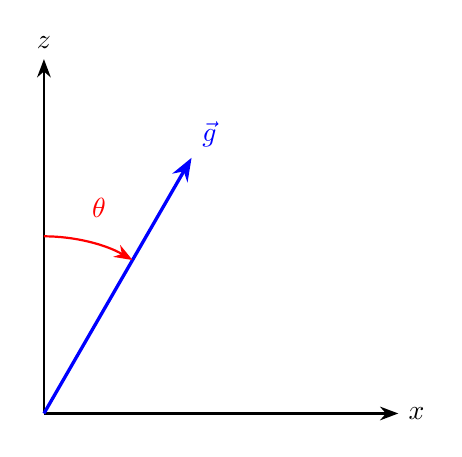
\begin{tikzpicture}[scale=1.5, >=Stealth]
				% Assi
				\draw[->, thick] (0,0) -- (3,0) node[right] {$x$};
				\draw[->, thick] (0,0) -- (0,3) node[above] {$z$};

				\draw[->, very thick, blue] (0,0) -- (60:2.5) node[above right] {$\vec{g}$};

				\draw[->, red, thick] (0,1.5) arc (90:60:1.5);

				\node[red] at (75:1.8) {$\theta$};
			\end{tikzpicture}
		\end{minipage}
		\hfill
		\begin{minipage}{0.45\textwidth}
			\centering
			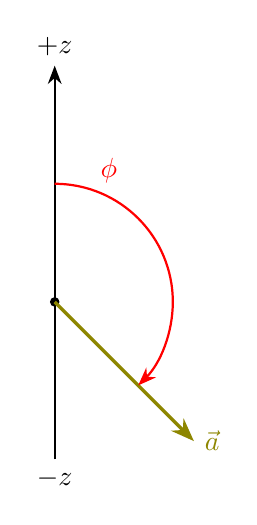
\begin{tikzpicture}[scale=1.0, >=Stealth]
				\draw[->, thick] (0,-2) -- (0,3) node[above] {$+z$};
				\node[below] at (0,-2) {$-z$};
				\filldraw (0,0) circle (1.5pt);
				.
				\draw[->, very thick, olive] (0,0) -- (-45:2.5) node[right] {$\vec{a}$};

				\draw[->, red, thick] (0,1.5) arc (90:-45:1.5);

				\node[red] at (67.5:1.8) {$\phi$};
			\end{tikzpicture}
		\end{minipage}
	\end{figure}

	\begin{gather}
		g_z = \cos{(\theta)} \quad ; \quad g_x = \sin{(\theta)} \label{eq:gz_gx_geom_def} \\
		g_0 = \cos{(\phi/2)} \quad ; \quad g_1 = \sin{(\phi/2)} \label{eq:g0_g1_geom_def} \\
		\text{so that} \quad g_0^2 - g_1^2 = \cos{(\phi)} \quad ; \quad 2g_0g_1 = \sin{(\phi)} \notag
	\end{gather}

	In this way we can reformulate :
	\begin{gather}
		g_{z}\left(g_{0}^{2} - g_{1}^{2} \right) + 2 g_{1} g_{0} g_{x} = 0 \notag \\
		\cos{(\theta)}\cos{(\phi)} + \sin{(\theta)}\sin{(\phi)} = 0 \notag \\
		\cos{(\theta - \phi)} = 0 \notag \\
		\theta - \phi = \frac{\pi}{2} \quad \rightarrow \quad \theta = \frac{\pi}{2} + \phi
		\label{eq:g_equivalnce_geom_sol}
	\end{gather}

	Geometrically, this signifies that purely dissipative dynamics, in the Lindblad form, emerge only when the direction of the Collisional Interaction vector is perpendicular to the Ancilla's polarization vector on the Bloch sphere.

	\newpage

	To recover the two limits we have to set:

	\begin{itemize}
		\item Quantum Jump limit : $ g_z = 0 , g_x = 1 \, ; \, g_0 = 1 , g_1 = 0 \, ; \, \theta = 90° , \phi = 0° $
		\item State Diffusion limit : $ g_z = 1 , g_x = 0 \, ; \, g_0 = 1/\sqrt{2} , g_1 = 1/\sqrt{2} \, ; \, \theta = 0° , \phi = 90° $
	\end{itemize}

	It is worth noting that the resulting Master Equation that lead to the Lindblad form with $ \mathcal{L}_k = \sigma_{z} $ describes a Pure Dephasing dynamic, where the Collisional environment destroys the quantum Coherence of the system, without inducing population transfer (energy relaxation).

	\begin{equation}
		\dot{\rho_S} = \Gamma \left(\sigma_{z} \rho_S \sigma_{z} - \rho_S \right) \quad \text{Pure Dephasing}
		\label{eq:lindblad_pure_deph_recover}
	\end{equation}

	It's possible to redefine the $ \mathcal{M} $ operators using the relations between the \textit{g} parameters :
	\begin{align}
		\mathcal{M}_{0}^{j}&= g_0 \cos(c_j \Delta t) \mathbb{I}^{j} + i g_1 \sin(c_j \Delta t) \sigma_{z}^{j} \label{eq:M0_simplified} \\
		\mathcal{M}_{1}^{j} &= g_1 \cos(c_j \Delta t) \mathbb{I}^{j} - i g_0 \sin(c_j \Delta t) \sigma_{z}^{j} \label{eq:M1_simplified}
	\end{align}

	and on the other way :
	\begin{align}
		\mathcal{M}_{0}^{j} &= \sqrt{\frac{1+g_x}{2}} \cos(c_j \Delta t) \mathbb{I}^{j} + i \sqrt{\frac{1-g_x}{2}} \sin(c_j \Delta t) \sigma_{z}^{j} \\
		\mathcal{M}_{1}^{j} &= \sqrt{\frac{1-g_x}{2}} \cos(c_j \Delta t) \mathbb{I}^{j} - i \sqrt{\frac{1+g_x}{2}} \sin(c_j \Delta t) \sigma_{z}^{j}
	\end{align}

	\subsubsection{Focus on the $ 3^{rd} $ term}
	Let's check what happens if we don't erase the last term in Eq.46

	\begin{equation}
		i \Big( g_{z}\left(g_{0}^{2} - g_{1}^{2} \right) + 2 g_{1} g_{0} g_{x} \Big) \cos{\left(c_j \Delta t \right)} \sin{\left(c_j \Delta t \right)} \Big[\rho_S , \sigma_{z} \Big]
		\label{eq:3_term}
	\end{equation}
	\\
	As seen so far in section 2.2.3 we can recover the complete form of
	\begin{equation}
		\rho_S' = \rho_S (t + \Delta t) = \mathcal{U}_{tot}(\Delta t) \rho_S (t) = \exp{\left[-i \, \left(\mathcal{H}_{Exc} + \mathcal{H}_{Coll} \right) \, \Delta t \right]} \rho_S (t)
		\label{eq:rho_S_LVN_comp_evo}
	\end{equation}\\
	by Trottarization of the $ \mathcal{U}_{tot} = e^{-i \, \mathcal{H}_{Exc} \, \Delta t } \, e^{-i \, \mathcal{H}_{Coll} \, \Delta t }  $ (with an error $ \mathcal{O}\left(\Delta t^2\right) $) .\\
	So that we can sequently apply the two exponential operator, in particular we already know the result given by the Collsional term, i.e. Eq.46 at which we can apply the Exciton term; but first we need to explicit its $ \lim{\Delta t \rightarrow 0} $ :

	\begin{equation}
		\lim\limits_{\Delta t \rightarrow 0} \, \rho_S' = \rho_S + c_{j}^{2} \Delta t ^{2} \left( \sigma_{z} \rho_S \sigma_{z} - \rho_S \right) + i \Big( g_{z}\left(g_{0}^{2} - g_{1}^{2} \right) + 2 g_{1} g_{0} g_{x} \Big) c_j \Delta t [\rho_S , \sigma_{z} \Big]
		\label{eq:lim0_comp_rho_s}
	\end{equation}

	Since : \begin{itemize}
	\item $ \cos{\left(c_j \Delta t \right)}^{2} \approx 1 - c_{j}^{2} \Delta t ^{2} $
	\item $ \sin{\left(c_j \Delta t \right)}^{2} \approx c_{j}^{2} \Delta t ^{2} $
	\item $ \cos{\left(c_j \Delta t \right)} \sin{\left(c_j \Delta t \right)} \approx 1 \cdot c_j \Delta t  $
\end{itemize}
Now defining $ \Gamma_{j} = c_{j}^{2} \Delta t $ and $ \mathcal{K} = \Big( g_{z}\left(g_{0}^{2} - g_{1}^{2} \right) + 2 g_{1} g_{0} g_{x} \Big) c_j $ , we can rewrite more comfortably :
\begin{equation}
	\rho_S' = \rho_S + \Gamma_{j} \Delta t \left( \sigma_{z} \rho_S \sigma_{z} - \rho_S \right) + i \mathcal{K} \Delta t \Big[ \rho_S , \sigma_{z} \Big]
	\label{eq:compact_rho_S_evo}
\end{equation}

We can now apply the evolution due to the $ \mathcal{H}_{Exc} $ which in the first order approximation reduces to the Liouville - von Neumann equation :

\begin{gather}
	\rho_S (t + \Delta t) = e^{-i \, \mathcal{H}_{Exc} \Delta t} \rho_S' e^{\, i \, \mathcal{H}_{Exc} \Delta t} \approx \rho_S' - i \Big[\mathcal{H}_{Exc} , \rho_S' \Big] \Delta t \notag \\
	= \rho_S' - i \Big[ \mathcal{H}_{Exc} \, , \, \rho_S + \Gamma_{j} \Delta t \left( \sigma_{z} \rho_S \sigma_{z} - \rho_S \right) + i \mathcal{K} \Delta t \Big[ \rho_S , \sigma_{z} \Big] \Big] \Delta t
	\label{eq:compact_complete_rho_S_evo}
\end{gather}

Considering again $ \lim \Delta t \rightarrow 0 $ we can neglect the term quadratic in $ \Delta t $

\begin{gather}
	\rho_S (t + \Delta t) \approx \rho_S + \Gamma_{j} \Delta t \left( \sigma_{z} \rho_S (t) \sigma_{z} - \rho_S (t) \right) - i \mathcal{K} \Delta t \Big[ \sigma_{z} , \rho_S (t) \Big] - i \Big[ \mathcal{H}_{Exc} \, , \, \rho_S (t) \Big] \notag \\
	\frac{\rho_S (t + \Delta t) - \rho_S (t)}{\Delta t} \approx \Gamma_{j} \left( \sigma_{z} \rho_S \sigma_{z} - \rho_S \right) - i \Big[ \left( \mathcal{H}_{Exc} + \mathcal{K} \sigma_z \right), \rho_S \Big] \notag \\
	\dot{\rho_S} = \Gamma_{j} \left( \sigma_{z} \rho_S \sigma_{z} - \rho_S \right) - i \Big[ \left( \mathcal{H}_{Exc} + \mathcal{K} \sigma_z \right), \rho_S \Big]
	\label{eq:final_complete_form_rho_S_evo}
\end{gather}

Remembering that $ \mathcal{K} = \Big( g_{z}\left(g_{0}^{2} - g_{1}^{2} \right) + 2 g_{1} g_{0} g_{x} \Big) c_j $ derives from the $ 3^{rd} $ term in Eq.46 it's clear that this term act as a shift in the Energy of the system's site \{ Lamb Shift ?\}. \\
But we need to be careful since we have a $ c_j = \sqrt{\Gamma_j / \Delta t} $ in the $ \mathcal{K} $ definition and applying the $ \lim \Delta t \rightarrow 0 $ it would diverge. \\
To get around this problem we can redefine the components of the direction of $ \mathcal{H}_{Coll} $ as function of $ \Delta t $ :

\begin{equation}
	g_z = \Gamma_{z} \sqrt{\Delta t} \quad ; \quad g_x = \Gamma_{x} \sqrt{\Delta t}
	\label{eq:gz_gx_reformulation}
\end{equation}

so that Eq.40 becomes
\begin{align}
	\sqrt{g_{z}^{2} + g_{x}^{2}} = \sqrt{\Gamma_{z}^{2} + \Gamma_{x}^{2} } \sqrt{\Delta t} = 1
	\label{eq:geom_constrain}
\end{align}

and $ \mathcal{K} $ becomes independent from $ \Delta t $

\begin{align}
	\mathcal{K} &= \frac{\sqrt{\Gamma_{j}}}{\cancel{\sqrt{\Delta t}}} \cdot \cancel{\sqrt{\Delta t}} \left( \Gamma_{z}\left(g_{0}^{2} - g_{1}^{2} \right) + 2 g_{1} g_{0} \Gamma_{x}\right) \notag \\
	&= \sqrt{\Gamma_{j}} \left( \Gamma_{z}\left(g_{0}^{2} - g_{1}^{2} \right) + 2 g_{1} g_{0} \Gamma_{x}\right)
	\label{eq:K_term_refomrulation}
\end{align}

This solution is coherent with the definition used for $ c_j = \sqrt{\Gamma_j / \Delta t} $ and the Collisional Hamiltonian becomes :

\begin{equation}
	\mathcal{H}_{Coll} = \sqrt{\Gamma_{j}} \, \sigma_{z}^{j} \otimes \left( \Gamma_{z} \sigma_{z}^{a_j} + \Gamma_{x} \sigma_{x}^{a_j} \right)
	\label{eq:H_coll_refomrulation}
\end{equation}

\subsubsection{Probability of measuring the Ancilla's states}

After the collision the Ancilla could be either in state $ \ket{0_a} $ or $ \ket{1_a} $ with a finite probability which is generally given by:

\begin{align}
	P_{0_{a}} = Tr_{S} \left[\braket{0_a|\Psi'}\braket{\Psi'|0_a} \right] \\
	P_{1_{a}} = Tr_{S} \left[\braket{1_a|\Psi'}\braket{\Psi'|1_a} \right]
\end{align}

To evaluate this values we first redefine the operators $ \mathcal{M}_{0} $ and $ \mathcal{M}_{1} $ using the value :
\begin{align}
	a_{0} = g_{0} \cos{\left(c_{j}\Delta t\right)} \quad ; \quad b_{0} = \left(g_{0} g_{z} + g_{1}g_{x} \right) \sin{\left(c_{j}\Delta t\right)} \label{eq_a0_b0_def} \\
	a_{1} = g_{1} \cos{\left(c_{j}\Delta t\right)} \quad ; \quad b_{1} = \left(g_{0} g_{x} - g_{1}g_{z} \right) \sin{\left(c_{j}\Delta t\right)} \label{eq_a01b1_def}
\end{align}
so that :
\begin{align}
	\mathcal{M}_{0}^{j} = a_{0} \mathbb{I}^{j} -i b_{0} \sigma_{z}^{j} \quad ; \quad \mathcal{M}_{0}^{j \dagger} = a_{0} \mathbb{I}^{j} + i b_{0} \sigma_{z}^{j} \label{eq_M0_def} \\
	\mathcal{M}_{1}^{j} = a_{1} \mathbb{I}^{j} -i b_{1} \sigma_{z}^{j} \quad ; \quad \mathcal{M}_{1}^{j \dagger} = a_{1} \mathbb{I}^{j} + i b_{1} \sigma_{z}^{j}
	\label{eq_M1_def}
\end{align}

If we expand Eq.\ref{eq:MO_M1_rho_int} using this definition :
\begin{align}
	\rho' &= \ket{\Psi'}\bra{\Psi'} = \mathcal{M}_{0}^{j} \rho_S \mathcal{M}_{0}^{j \dagger} \otimes \ket{0_a}\bra{0_a} + \mathcal{M}_{1}^{j} \rho_S \mathcal{M}_{1}^{j \dagger} \otimes \ket{1_a} \bra{1_a} \notag \\
	& \quad + \mathcal{M}_{0}^{j} \rho_S \mathcal{M}_{1}^{j \dagger} \otimes \ket{0_a} \bra{1_a} + \mathcal{M}_{1}^{j} \rho_S \mathcal{M}_{0}^{j \dagger} \otimes \ket{1_a} \bra{0_a} \notag \\
	& = \left(a_{0} \mathbb{I}^{j} - i b_{0} \sigma_{z}^{j}\right) \ket{\Psi_{S}}\bra{\Psi_{S}} \left(a_{0} \mathbb{I}^{j} + i b_{0} \sigma_{z}^{j}\right) \otimes \ket{0_{a}} \bra{0_{a}} \notag \\
	& + \left(a_{1} \mathbb{I}^{j} - i b_{1} \sigma_{z}^{j}\right) \ket{\Psi_{S}}\bra{\Psi_{S}} \left(a_{1} \mathbb{I}^{j} + i b_{1} \sigma_{z}^{j}\right) \otimes \ket{1_{a}} \bra{1_{a}} \notag \\
	& + \left(a_{0} \mathbb{I}^{j} - i b_{0} \sigma_{z}^{j}\right) \ket{\Psi_{S}}\bra{\Psi_{S}} \left(a_{1} \mathbb{I}^{j} + i b_{1} \sigma_{z}^{j}\right) \otimes \ket{0_{a}} \bra{1_{a}} \notag \\
	& + \left(a_{1} \mathbb{I}^{j} - i b_{1} \sigma_{z}^{j}\right) \ket{\Psi_{S}}\bra{\Psi_{S}} \left(a_{0} \mathbb{I}^{j} + i b_{0} \sigma_{z}^{j}\right) \otimes \ket{1_{a}} \bra{0_{a}} \notag \\
	& = \Big[ \left|a_{0}\right|^{2} \ket{\Psi_{S}}\bra{\Psi_{S}} + \left|b_{0}\right|^{2} \sigma_{z}^{j}\ket{\Psi_{S}}\bra{\Psi_{S}}\sigma_{z}^{j} + i a_{0}b_{0}\ket{\Psi_{S}}\bra{\Psi_{S}}\sigma_{z}^{j} -  i a_{0}b_{0} \sigma_{z}^{j} \ket{\Psi_{S}}\bra{\Psi_{S}} \Big] \otimes \ket{0_{a}} \bra{0_{a}} \notag \\
	& + \Big[ \left|a_{1}\right|^{2} \ket{\Psi_{S}}\bra{\Psi_{S}} + \left|b_{1}\right|^{2} \sigma_{z}^{j}\ket{\Psi_{S}}\bra{\Psi_{S}}\sigma_{z}^{j} + i a_{1}b_{1}\ket{\Psi_{S}}\bra{\Psi_{S}}\sigma_{z}^{j} -  i a_{1}b_{1} \sigma_{z}^{j} \ket{\Psi_{S}}\bra{\Psi_{S}} \Big] \otimes \ket{1_{a}} \bra{1_{a}} \notag \\
	& + \Big[ a_{0} a_{1} \ket{\Psi_{S}}\bra{\Psi_{S}} + b_{0} b_{1}  \sigma_{z}^{j}\ket{\Psi_{S}}\bra{\Psi_{S}}\sigma_{z}^{j} + i a_{0}b_{1}\ket{\Psi_{S}}\bra{\Psi_{S}}\sigma_{z}^{j} -  i a_{1}b_{0} \sigma_{z}^{j} \ket{\Psi_{S}}\bra{\Psi_{S}} \Big] \otimes \ket{0_{a}} \bra{1_{a}} \notag \\
	& + \Big[ a_{1} a_{0} \ket{\Psi_{S}}\bra{\Psi_{S}} + b_{1} b_{0}  \sigma_{z}^{j}\ket{\Psi_{S}}\bra{\Psi_{S}}\sigma_{z}^{j} + i a_{1}b_{0}\ket{\Psi_{S}}\bra{\Psi_{S}}\sigma_{z}^{j} -  i a_{0}b_{1} \sigma_{z}^{j} \ket{\Psi_{S}}\bra{\Psi_{S}} \Big] \otimes \ket{1_{a}} \bra{0_{a}} \notag
\end{align}
Now we can calculate :
\begin{align}
	P_{0_{a}} & = Tr_{S} \left[\braket{0_a|\Psi'}\braket{\Psi'|0_a} 	\right] \notag \\
	& = Tr_{S} \Big[ \left|a_{0}\right|^{2} 	\ket{\Psi_{S}}\bra{\Psi_{S}} + \left|b_{0}\right|^{2} \sigma_{z}^{j} \ket{\Psi_{S}}\bra{\Psi_{S}} \sigma_{z}^{j} + i a_{0}b_{0}\ket{\Psi_{S}}\bra{\Psi_{S}} \sigma_{z}^{j} -  i a_{0}b_{0} \sigma_{z}^{j} \ket{\Psi_{S}}\bra{\Psi_{S}} \Big] \notag \\
	& = \left|a_{0}\right|^{2} Tr_{S} \Big[ 	\ket{\Psi_{S}}\bra{\Psi_{S}} \Big] + \left|b_{0}\right|^{2} Tr_{S} \Big[ \sigma_{z}^{j} \ket{\Psi_{S}}\bra{\Psi_{S}} \sigma_{z}^{j} \Big] \notag \\
	& \quad + i \,a_{0} b_{0} \, Tr_{S} \Big[ 	\ket{\Psi_{S}}\bra{\Psi_{S}} \sigma_{z}^{j} \Big] - i \, a_{0} b_{0} \, Tr_{S} \Big[ \sigma_{z}^{j} \ket{\Psi_{S}}\bra{\Psi_{S}} \Big] \notag \\
	& \big(\text{remembering that} \quad Tr \left[ABC\right] = Tr 	\left[CAB\right] \quad \text{and} \quad \sigma_{z} \sigma_{z} = \mathbb{I} \big) \notag \\
	& = \left|a_{0}\right|^{2} Tr_{S} \Big[ 	\ket{\Psi_{S}}\bra{\Psi_{S}} \Big] + \left|b_{0}\right|^{2} Tr_{S} \Big[  \ket{\Psi_{S}}\bra{\Psi_{S}} \Big] \notag \\
	& \quad + \cancel{i \,a_{0} b_{0} \, Tr_{S} \Big[ \sigma_{z}^{j} 	\ket{\Psi_{S}}\bra{\Psi_{S}} \Big]} \cancel{- i \, a_{0} b_{0} \, Tr_{S} \Big[ \sigma_{z}^{j} \ket{\Psi_{S}}\bra{\Psi_{S}} \Big]} \notag \\
	P_{0_{a}} & = \left|a_{0}\right|^{2} + \left|b_{0}\right|^{2} = 	g_{0}^{2} \cos^{2}{\left(c_{j}\Delta t\right)} + \left(g_{0} g_{z} + g_{1}g_{x} \right)^{2} \sin^{2}{\left(c_{j}\Delta t\right)} \label{eq_P0_value} \\
	\notag \\
	& \text{and the same for :} \notag \\
	\notag \\
	P_{1_{a}} &= \left|a_{1}\right|^{2} + \left|b_{1}\right|^{2} = 	g_{1}^{2} \cos^{2}{\left(c_{j}\Delta t\right)} + \left(g_{0} g_{x} - g_{1}g_{z} \right)^{2} \sin^{2}{\left(c_{j}\Delta t\right)} \label{eq_P1_value}
\end{align}

Or in another formulation :
\begin{align}
	P_{0_a} & = g_0^2 \cos^2(c_j \Delta t) + g_1^2 \sin^2(c_j \Delta t) \label{eq:P0a_final} \\
	P_{1_a} & = g_1^2 \cos^2(c_j \Delta t) + g_0^2 \sin^2(c_j \Delta t) \label{eq:P1a_final}
\end{align}

So setting the \textit{g} parameter directly defines the probability of measuring a different Ancilla's state; we could check if this definition lead back to the probability obtained in the Quantum Jump and Coherent limit:

\begin{itemize}
	\item QJ : $ g_z = 0 , g_x = 1 \, ; \, g_0 = 1 , g_1 = 0 \, ; \, \theta = 90° , \phi = 0° \rightarrow P_{0_{a}} = \cos^{2}{\left(c_{j}\Delta t\right)} \, ; \, P_{1_{a}} = \sin^{2}{\left(c_{j}\Delta t\right)} $
	\item Diff : $ g_z = 1 , g_x = 0 \, ; \, g_0 = 1/\sqrt{2} , g_1 = 1/\sqrt{2} \, ; \, \theta = 0° , \phi = 90° \rightarrow P_{0_{a}} = \frac{1}{2} \, ; \, P_{1_{a}} = \frac{1}{2} $
\end{itemize}

Now we could try to see how the probability of measuring the two different Ancilla's states changes varying the \textit{g} values, for example as function of the angle $ \theta $ (with $ \theta = \frac{\pi}{2} + \phi $) :

%\graphicspath{ {/home/francesco/Collisional_Methods/Results/Plot/Probability} }
\begin{figure}[H]
	\centering
	\includegraphics[width=0.7\textwidth]{{Prob(theta)}.png}
	\caption{Probability of measuring the two different Ancilla's states $\ket{0_{a}}$ and $\ket{1_{a}}$, as function of the $\theta$ angle, which defines the direction of the $\mathcal{H}_{\text{Coll}}$ respect to z axis}
	\label{fig:prob_theta}
\end{figure}

As observed, for $\theta = 90^\circ$ (Quantum Jump limit), the probability of measuring $\ket{0_{a}}$ is $P_{0_{a}}\approx 1$. This corresponds to the application of the identity operator $\mathbb{I}^{j}$ on the system's wf; conversely, the probability of measuring $\ket{1_{a}}$ is $P_{1_{a}}\approx 0$, which corresponds to the application of $\sigma_{z}^{j}$.

On the other hand, for $\theta = 0^\circ$ (Diffusional limit), both probabilities are approximately $1/2$. In this regime, the system's wf undergoes a continuous modification regardless of the outcome ($\ket{0_{a}}$ or $\ket{1_{a}}$), with the modification weighted by a small factor and differing by a sign.\\

\newpage

Now the question that arises is, if both the two unraveling has to give back the same average dynamic, but

\begin{itemize}
	\item in the QJ limit we have a small probability to apply a big change in the System's wf ;
	\item in the Diff. limit we always apply a variation to the System's wf but this produces a small change.
\end{itemize}

Is it possible to quantify a quantity that defines the intensity of the variation applied to the System's wf after the collision? Is it possible to define it as a function of the \textit{g} parameters? And therefore, what would its behavior be with respect to the angle theta?

\subsubsection{Kraus Operators}
\label{sub:focus_on_M0_M1}
Remember that:
\begin{align*}
	\mathcal{M}_{0}^{j} &= g_0 \cos(c_j \Delta t) \mathbb{I}^{j} + i g_1 \sin(c_j \Delta t) \sigma_{z}^{j} \\
	\mathcal{M}_0^{j \dagger} &= g_0 \cos(c_j \Delta t) \mathbb{I}^{j} - i g_1 \sin(c_j \Delta t) \sigma_{z}^{j} \\
	\mathcal{M}_{1}^{j} &= g_1 \cos(c_j \Delta t) \mathbb{I}^{j} - i g_0 \sin(c_j \Delta t) \sigma_{z}^{j} \\
	\mathcal{M}_1^{j \dagger} &= g_1 \cos(c_j \Delta t) \mathbb{I}^{j} + i g_0 \sin(c_j \Delta t) \sigma_{z}^{j}
\end{align*}

\label{subsub:Kraus_Operators}
$ \mathcal{M}_0 $ and $ \mathcal{M}_1 $ could be seen as \textit{Kraus Operators}, as defined in the \textit{Petruccione} :
\begin{align}
	\rho_{S} \left(t\right) &= \mathcal{V}\left(t\right) \rho_{S} \left(0\right) = Tr_{B} \Big\{ \mathcal{U}\left(t, t_0\right) \Big[ \rho_{S} \otimes \rho_{B} \Big] \mathcal{U}^{\dagger}\left(t, t_0\right) \Big\} \\
	&\left( \rho_{B} = \sum_{\alpha}{\lambda_{\alpha} \ket{\varphi_{\alpha}} \bra{\varphi_{\alpha}}} \quad \text{and} \quad Tr_{B} = \sum_{\beta}{\bra{\varphi_{\beta}} \dots \ket{\varphi_{\beta}}} \right) \notag \\
	&= \sum_{\alpha}{\sum_{\beta}{\lambda_{\alpha}\bra{\varphi_{\beta}} \mathcal{U}\left(t, t_0\right) \left[ \rho_{S} \otimes \ket{\varphi_{\alpha}} \bra{\varphi_{\alpha}} \right]  \mathcal{U}^{\dagger}\left(t, t_0\right) \ket{\varphi_{\beta}} }} \notag \\
	&= \sum_{\alpha, \beta}{ \mathcal{W}_{\alpha, \beta} \left(t\right) \rho_{S} \mathcal{W}^{\dagger}_{\alpha, \beta} \left(t\right) }
	\label{eq:dynamical_map_kraus_operators}
\end{align}
where $ \mathcal{W}_{\alpha, \beta} \left(t\right) $ are operators that act on the \textit{wf} of the system solely, defining the evolution conditioned by the measurement of the bath state; this operators take the form :
\begin{equation}
	\mathcal{W}_{\alpha, \beta} \left(t\right) = \sqrt{\lambda_{\alpha}} \bra{\varphi_{\beta}}  \mathcal{U}\left(t, t_0\right) \ket{\varphi_{\alpha}}
	\label{eq:general_kraus_operators}
\end{equation}
The set of operators $\{ \mathcal{W}_{\alpha, \beta} \}$ formally constitutes a set of \textit{Kraus Operators}, where the standard single Kraus index is represented by the pair $(\alpha, \beta)$. Since they satisfy the completeness relation $\sum_{\alpha, \beta} \mathcal{W}_{\alpha, \beta}^\dagger \mathcal{W}_{\alpha, \beta} = \mathbb{I}_S$, they guarantee a Completely Positive and Trace-Preserving (CPTP) map.

\newpage

In our specific model, the Ancilla is initialized in a pure coherent superposition state, defined as $\ket{\varphi_{a}} =  \ket{\phi_a} = g_0 \ket{0_a} + g_1 \ket{1_a}$. \\
To derive the explicit form of the Kraus operators for this dynamics, we start by constructing the density matrix of the environment $\rho_B$ and analyzing its spectral decomposition:
\begin{equation}
	\rho_B = \ket{\varphi_a}\bra{\varphi_a} =
	\begin{pmatrix}
	|g_0|^2 & g_0 g_1^* \\
	g_0^* g_1 & |g_1|^2
	\end{pmatrix}
\end{equation}
The spectral decomposition of the ancilla's density matrix $\rho_B = \ket{\varphi_{a}}\bra{\varphi_{a}}$ yields the following eigenvalues and eigenvectors:

\begin{itemize}
	\item $\lambda_1 = 1 \rightarrow \ket{\varphi_1} = g_0 \ket{0_a} + g_1 \ket{1_a} $

	\item $\lambda_2 = 0 \rightarrow \ket{\varphi_2} = g_1^* \ket{0_a} - g_0^* \ket{1_a} $
\end{itemize}
Since $ \lambda_2 = 0 $ only two operators $ \mathcal{W}_{\alpha, \beta} $ are obtained, in particular, using the bases $ \{ \ket{0_{a}}, \ket{1_{a}} \} $ for the Trace, one gets from Eq.\ref{eq:general_kraus_operators}
\begin{gather}
	\mathcal{W}_{0, \varphi_{1}} = g_0 \cos{\left(c_j \Delta t \right)} \mathbb{I}^{j} - i \left(g_0 g_z + g_1 g_x \right) \sin{\left(c_j \Delta t \right)} \sigma_{z}^{j} \equiv \mathcal{M}_{0}^{j} \\
	\mathcal{W}_{1, \varphi_{1}} = g_1 \cos{\left(c_j \Delta t \right)} \mathbb{I}^{j} - i \left(g_0 g_x - g_1 g_z \right) \sin{\left(c_j \Delta t \right)} \sigma_{z}^{j} \equiv \mathcal{M}_{1}^{j}
\end{gather}
To confirm their validity as Kraus operators, they must satisfy the \textit{Completeness Relation}:
\begin{equation}
	\sum_{\mu} \mathcal{M}_{\mu}^{j \dagger} \mathcal{M}_{\mu}^{j} = \mathcal{M}_{0}^{j \dagger}\mathcal{M}_{0}^{j} + \mathcal{M}_{1}^{j \dagger}\mathcal{M}_{1}^{j} = \mathbb{I}^{j}
	\label{eq:completeness_relation}
\end{equation}
This condition ensures that the dynamical map is trace-preserving, reflecting the conservation of total probability during the collisional process.
In our case we get:
\begin{gather}
	\mathcal{M}_{0}^{j \dagger}\mathcal{M}_{0}^{j} = [g_0^2 \cos^2(c_j \Delta t) + g_1^2 \sin^2(c_j \Delta t)] \mathbb{I}^{j} \notag \\
	\mathcal{M}_{1}^{j \dagger}\mathcal{M}_{1}^{j} = [g_1^2 \cos^2(c_j \Delta t) + g_0^2 \sin^2(c_j \Delta t)] \mathbb{I}^{j} \notag \\
	\textit{so that} \notag \\
	\mathcal{M}_{0}^{j \dagger}\mathcal{M}_{0}^{j} + \mathcal{M}_{1}^{j \dagger}\mathcal{M}_{1}^{j} = \left[ g_0^2 \cos^2(c_j \Delta t) + g_1^2 \sin^2(c_j \Delta t) + g_1^2 \cos^2(c_j \Delta t) + g_0^2 \sin^2(c_j \Delta t) \right] \mathbb{I}^{j} \notag \\
	= \left[\left( g_{0}^{2} + g_{1}^{2} \right)\cos^2(c_j \Delta t) + \left( g_{0}^{2} + g_{1}^{2} \right)\sin^2(c_j \Delta t)\right] \mathbb{I}^{j} \notag \\
	= \left[\cos^2(c_j \Delta t) + \sin^2(c_j \Delta t)\right] \mathbb{I}^{j} = \mathbb{I}^{j}.
\end{gather}
Note that : 
\begin{gather}
	\mathcal{M}_{0}^{j \dagger}\mathcal{M}_{0}^{j}  = P_{0_{a}} \mathbb{I} \notag \\
	\mathcal{M}_{1}^{j \dagger}\mathcal{M}_{1}^{j}  = P_{1_{a}} \mathbb{I} \notag
\end{gather}
When we apply $ \mathcal{M}_{0}^{j} \ket{\psi_{S}} $ we're reducing the norm of the state vector; the square of the norm is given by $ \bra{\psi_{S}} \mathcal{M}_0^{\dagger}\mathcal{M}_{0}^{j} \ket{\psi_{S}} = P_{0_{a}} $
so that :
\begin{equation}
	\ket{\psi_{S}^{Post}} = \frac{\mathcal{M}_{0}^{j}}{\sqrt{P_{0_{a}}}} \ket{\psi_{S}}
\end{equation}
since the bare \textit{Kraus Operators} inherently include the event probability, we must divide by $ \sqrt{P_{0_{a}}} $ to correctly normalize the post-collision state.
 
\newpage 
So far we've seen only the \textbf{Single Site Kraus Operators}, i.e. the operators acting only on one of the two site. In an analogous way we can derive the \textit{Kraus Operators} acting on both the site, i.e. on the total wave function of the system. It's important to specify that, since we're analyzing only the Collisional evolution, one has to remember that before this one there's the coherent evolution via the excitonic Hamiltonian, which can generate entanglement between the wave functions of the single site, so in this case the Total System wave function becomes :
\begin{gather}
	\ket{\Psi_{S}} = c_{00} \ket{0_{1}0_{2}} + c_{10} \ket{1_{1}0_{2}} + c_{01} \ket{0_{1}1_{2}} + c_{11} \ket{1_{1}1_{2}} \\
	\left(\text{where}  \ket{0_{1}0_{2}} = \ket{0_{1}} \otimes \ket{0_{2}}\right) \notag
\end{gather}
For the Ancilla instead, since every site has and independent reservoir of Ancillas and before the collision the ancilla is always taken in its initial state, i.e. without any entanglement, the total ancilla \textit{wf} reads :
\begin{gather}
	\ket{\Phi_{A}} = \ket{\phi_{a}^{1}} \otimes \ket{\phi_{a}^{2}} \\
	\text{where} \ket{\phi_{a}^{1}} = g_{0} \ket{0_{a}} + g_{1} \ket{1_{a}} =  \ket{\phi_{a}^{2}} \notag
\end{gather}
As already done for the single site, to obtain the Total \textit{Kraus Operators} we can start from the evolution of the total wf via :
\begin{gather}
	\mathcal{U}_{Coll}^{Tot} \left(\Delta t\right) = \exp{ -i \sum_{j}{\mathcal{H}_{Coll}^{j}} \Delta t } = \exp{-i \sum_{j}{c_{j} \sigma_{z}^{j} \otimes \left( g_{x} \sigma_{x}^{a_{j}} + g_{z} \sigma_{z}^{a_{j}} \right) \Delta t}} \notag \\
	\exp{ \left(-i \mathcal{H}_{Coll}^{1} \Delta t\right) } \exp{ \left(-i \mathcal{H}_{Coll}^{2} \Delta t\right) } = \mathcal{U}_{Coll}^{1} \mathcal{U}_{Coll}^{2}
\end{gather}
where it's important to remember that :
\begin{gather}
	\sigma_{z}^{1} = \sigma_{z} \otimes \mathbb{I} \quad ; \quad 	\sigma_{z}^{2} = \mathbb{I} \otimes \sigma_{z} \notag \\
	\left[ \mathcal{H}_{Coll}^{1}, \mathcal{H}_{Coll}^{2} \right] = 0
\end{gather}
this allows to define the evolution pf the total wave function as it follows : 
\begin{align}
	\ket{\Psi \left(t + \Delta t\right)} &= \mathcal{U}_{Coll}^{Tot} \ket{\Psi \left(t\right)} = \mathcal{U}_{Coll}^{1} \otimes \mathcal{U}_{Coll}^{2} \Big[ \left( c_{00} \ket{0_{1}0_{2}} + c_{10} \ket{1_{1}0_{2}} + c_{01} \ket{0_{1}1_{2}} + c_{11} \ket{1_{1}1_{2}} \right) \otimes \ket{\phi_{a}^{1}} \otimes \ket{\phi_{a}^{2}} \Big] \notag \\
	& = \mathcal{U}_{Coll}^{1} \otimes \mathcal{U}_{Coll}^{2} \Big[ c_{00} \left(\ket{0_{1}} \otimes \ket{\phi_{a}^{1}} \right) \otimes \left(\ket{0_{2}} \otimes \ket{\phi_{a}^{2}} \right) + c_{10} \left(\ket{1_{1}} \otimes \ket{\phi_{a}^{1}} \right) \otimes \left(\ket{0_{2}} \otimes \ket{\phi_{a}^{2}} \right) \notag \\
	& + c_{01} \left(\ket{0_{1}} \otimes \ket{\phi_{a}^{1}} \right) \otimes \left(\ket{1_{2}} \otimes \ket{\phi_{a}^{2}} \right) + c_{11} \left(\ket{1_{1}} \otimes \ket{\phi_{a}^{1}} \right) \otimes \left(\ket{1_{2}} \otimes \ket{\phi_{a}^{2}} \right) \Big]
	\label{eq:total_kraus_op_derivation_first_part}
\end{align}
let's focus on the first term in the square bracket, that reads:
\begin{align}
	& \mathcal{U}_{Coll}^{1} \otimes \mathcal{U}_{Coll}^{2} \left[ c_{00} \left(\ket{0_{1}} \otimes \ket{\phi_{a}^{1}} \right) \otimes \left(\ket{0_{2}} \otimes \ket{\phi_{a}^{2}} \right) \right] \notag \\
	& = c_{00} \left\{ \left[ \mathcal{U}_{Coll}^{1} \left(\ket{0_{1}} \otimes \ket{\phi_{a}^{1}} \right)\right] \otimes \left[ \mathcal{U}_{Coll}^{2}  \left(\ket{0_{2}} \otimes \ket{\phi_{a}^{2}} \right) \right] \right\} 
	\label{eq:first_term_complete_derivation}
\end{align}
and again on the first term in the curly brackets : 
\begin{align}
	&\mathcal{U}_{Coll}^{1} \left(\ket{0_{1}} \otimes \ket{\phi_{a}^{1}} \right) = \mathcal{U}_{Coll}^{1} \left(\ket{0_{1}} \otimes \left(  g_{0} \ket{0_{a}} + g_{1} \ket{1_{a}}  \right) \right) \notag \\ 
	&= g_{0} \mathcal{U}_{Coll}^{1} \ket{0_{1}} \otimes \ket{0_{a}} + g_{1} \mathcal{U}_{Coll}^{1} \ket{0_{1}} \otimes \ket{1_{a}} \notag \\ 
	& = \mathcal{M}_{0}^{1} \ket{0_{1}} \otimes \ket{0_{a}} + \mathcal{M}_{1}^{1} \ket{0_{1}} \otimes \ket{1_{a}}
	\label{eq:first_first_term_complete_derivation}
\end{align}
where the last equation is based on what was calculated in Eq.\ref{eq:MO_M1_psi_evo}. 

\newpage

This is valid for the second term of Eq.\ref{eq:first_term_complete_derivation} so that we obtain :
\begin{align}
	& \mathcal{U}_{Coll}^{1} \otimes \mathcal{U}_{Coll}^{2} \left[ c_{00} \left(\ket{0_{1}} \otimes \ket{\phi_{a}^{1}} \right) \otimes \left(\ket{0_{2}} \otimes \ket{\phi_{a}^{2}} \right) \right] = c_{00} \left\{ \left[ \mathcal{U}_{Coll}^{1} \left(\ket{0_{1}} \otimes \ket{\phi_{a}^{1}} \right)\right] \otimes \left[ \mathcal{U}_{Coll}^{2} \left(\ket{0_{2}} \otimes \ket{\phi_{a}^{2}} \right) \right] \right\} \notag \\
	& = c_{00} \left[ \mathcal{M}_{0}^{1} \ket{0_{1}} \otimes \ket{0_{a}} + \mathcal{M}_{1}^{1} \ket{0_{1}} \otimes \ket{1_{a}} \right] \otimes \left[ \mathcal{M}_{0}^{2} \ket{0_{2}} \otimes \ket{0_{a}} + \mathcal{M}_{1}^{2} \ket{0_{2}} \otimes \ket{1_{a}} \right] \notag \\
	& = c_{00} \Big[ \mathcal{M}_{0}^{1} \mathcal{M}_{0}^{2} \ket{0_{1}0_{2}} \ket{0_{a}^{1}0_{a}^{2}} + \mathcal{M}_{0}^{1} \mathcal{M}_{1}^{2} \ket{0_{1}0_{2}} \ket{0_{a}^{1}1_{a}^{2}} + \mathcal{M}_{1}^{1} \mathcal{M}_{0}^{2} \ket{0_{1}0_{2}} \ket{1_{a}^{1}0_{a}^{2}} + \mathcal{M}_{1}^{1} \mathcal{M}_{1}^{2} \ket{0_{1}0_{2}} \ket{1_{a}^{1}1_{a}^{2}} \Big] \notag
\end{align}
if we redefine :
\begin{gather*}
	\mathcal{M}_{00} = \mathcal{M}_{0}^{1} \otimes \mathcal{M}_{0}^{2} \\
	\mathcal{M}_{10} = \mathcal{M}_{1}^{1} \otimes \mathcal{M}_{0}^{2} \\
	\mathcal{M}_{01} = \mathcal{M}_{0}^{1} \otimes \mathcal{M}_{1}^{2} \\
	\mathcal{M}_{11} = \mathcal{M}_{1}^{1} \otimes \mathcal{M}_{1}^{2} 
\end{gather*}

This derivation, i.e. Eq.\ref{eq:first_term_complete_derivation}, is valid for every different term of the expansion of the Total System wave function : $ \ket{0_{1}0_{2}}, \ket{1_{1}0_{2}}, \ket{0_{1}1_{2}}, \ket{1_{1}1_{2}}  $. This because effectively $ \mathcal{M}_{\alpha, \beta} $ are \textit{Kraus Operators}, i.e. their form depends only on the Bath states. So Eq.\ref{eq:total_kraus_op_derivation_first_part} becomes :
\begin{align}
	\ket{\Psi \left( t + \Delta t\right)} &= c_{00} \Big[ \mathcal{M}_{0}^{1} \mathcal{M}_{0}^{2} \ket{0_{1}0_{2}} \otimes \ket{0_{a}^{1}0_{a}^{2}} + \mathcal{M}_{0}^{1} \mathcal{M}_{1}^{2} \ket{0_{1}0_{2}} \otimes \ket{0_{a}^{1}1_{a}^{2}} \notag \\
	& + \mathcal{M}_{1}^{1} \mathcal{M}_{0}^{2} \ket{0_{1}0_{2}} \otimes \ket{1_{a}^{1}0_{a}^{2}} + \mathcal{M}_{1}^{1} \mathcal{M}_{1}^{2} \ket{0_{1}0_{2}} \otimes \ket{1_{a}^{1}1_{a}^{2}} \Big] \notag \\
	&+ c_{10} \Big[ \mathcal{M}_{0}^{1} \mathcal{M}_{0}^{2} \ket{1_{1}0_{2}} \otimes \ket{0_{a}^{1}0_{a}^{2}} + \mathcal{M}_{0}^{1} \mathcal{M}_{1}^{2} \ket{1_{1}0_{2}} \otimes \ket{0_{a}^{1}1_{a}^{2}} \notag \\
	& + \mathcal{M}_{1}^{1} \mathcal{M}_{0}^{2} \ket{1_{1}0_{2}} \otimes \ket{1_{a}^{1}0_{a}^{2}} + \mathcal{M}_{1}^{1} \mathcal{M}_{1}^{2} \ket{1_{1}0_{2}} \otimes \ket{1_{a}^{1}1_{a}^{2}} \Big] \notag \\
	&+ c_{01} \Big[ \mathcal{M}_{0}^{1} \mathcal{M}_{0}^{2} \ket{0_{1}1_{2}} \otimes \ket{0_{a}^{1}0_{a}^{2}} + \mathcal{M}_{0}^{1} \mathcal{M}_{1}^{2} \ket{0_{1}1_{2}} \otimes \ket{0_{a}^{1}1_{a}^{2}} \notag \\
	& + \mathcal{M}_{1}^{1} \mathcal{M}_{0}^{2} \ket{0_{1}1_{2}} \otimes \ket{1_{a}^{1}0_{a}^{2}} + \mathcal{M}_{1}^{1} \mathcal{M}_{1}^{2} \ket{0_{1}1_{2}} \otimes \ket{1_{a}^{1}1_{a}^{2}} \Big] \notag \\
	&+ c_{11} \Big[ \mathcal{M}_{0}^{1} \mathcal{M}_{0}^{2} \ket{1_{1}1_{2}} \otimes \ket{0_{a}^{1}0_{a}^{2}} + \mathcal{M}_{0}^{1} \mathcal{M}_{1}^{2} \ket{1_{1}1_{2}} \otimes \ket{0_{a}^{1}1_{a}^{2}} \notag \\
	& + \mathcal{M}_{1}^{1} \mathcal{M}_{0}^{2} \ket{1_{1}1_{2}} \otimes \ket{1_{a}^{1}0_{a}^{2}} + \mathcal{M}_{1}^{1} \mathcal{M}_{1}^{2} \ket{1_{1}1_{2}} \otimes \ket{1_{a}^{1}1_{a}^{2}} \Big] \notag
\end{align}
that can be reformulated as :
\begin{align}
	\ket{\Psi \left( t + \Delta t\right)} &= \mathcal{M}_{00} \ket{\Psi_{S}} \otimes \ket{0_{a}^{1}0_{a}^{2}} + \mathcal{M}_{01} \ket{\Psi_{S}} \otimes \ket{0_{a}^{1}1_{a}^{2}} + \mathcal{M}_{10} \ket{\Psi_{S}} \otimes \ket{1_{a}^{1}0_{a}^{2}} + \mathcal{M}_{11} \ket{\Psi_{S}} \otimes \ket{1_{a}^{1}1_{a}^{2}} \notag \\
	& = \sum_{\alpha,\beta = 0,1}{\mathcal{M}_{\alpha, \beta} \ket{\Psi_{S}} \otimes \ket{\alpha_{a}^{1}\beta_{a}^{2}} }
	\label{eq:final_evo_via_total_kraus_op}
\end{align}
We can now explicit the form of $ \mathcal{M}_{\alpha, \beta} $ we obtain :
\begin{align}
	\mathcal{M}_{00} &= g_0^2 \cos(c_1 \Delta t) \cos(c_2 \Delta t) \mathbb{I} - g_1^2 \sin(c_1 \Delta t) \sin(c_2 \Delta t) \sigma_z \otimes \sigma_z \notag \\
	&+ i g_0 g_1 \sin(c_1 \Delta t) \cos(c_2 \Delta t) \sigma_z^1 + i g_0 g_1 \cos(c_1 \Delta t) \sin(c_2 \Delta t) \sigma_z^2\\
	\mathcal{M}_{01} &= g_0 g_1 \cos(c_1 \Delta t) \cos(c_2 \Delta t) \mathbb{I} + g_0 g_1 \sin(c_1 \Delta t) \sin(c_2 \Delta t) \sigma_z \otimes \sigma_z \notag \\
	& + i g_1^2 \sin(c_1 \Delta t) \cos(c_2 \Delta t) \sigma_z^1 - i g_0^2 \cos(c_1 \Delta t) \sin(c_2 \Delta t) \sigma_z^2 \\
	\mathcal{M}_{10} &= g_0 g_1 \cos(c_1 \Delta t) \cos(c_2 \Delta t) \mathbb{I} + g_0 g_1 \sin(c_1 \Delta t) \sin(c_2 \Delta t) \sigma_z \otimes \sigma_z \notag \\
	& - i g_0^2 \sin(c_1 \Delta t) \cos(c_2 \Delta t) \sigma_z^1 + i g_1^2 \cos(c_1 \Delta t) \sin(c_2 \Delta t) \sigma_z^2 \\
	\mathcal{M}_{11} &= g_1^2 \cos(c_1 \Delta t) \cos(c_2 \Delta t) \mathbb{I} - g_0^2 \sin(c_1 \Delta t) \sin(c_2 \Delta t) \sigma_z \otimes \sigma_z \notag \\
	& - i g_0 g_1 \sin(c_1 \Delta t) \cos(c_2 \Delta t) \sigma_z^1 - i g_0 g_1 \cos(c_1 \Delta t) \sin(c_2 \Delta t) \sigma_z^2
\end{align}
since $ \sigma_z \otimes \mathbb{I} \, \mathbb{I} \otimes \sigma_z = \sigma_z \otimes \sigma_z $. Considering $ c_1 = c_2 $, which is the case needed to reproduce the dephasing Lindblad effect it simplifies as :
\begin{align}
	\mathcal{M}_{00} &= g_0^2 \cos^2(c \Delta t) (\mathbb{I} \otimes \mathbb{I}) - g_1^2 \sin^2(c \Delta t) (\sigma_z \otimes \sigma_z) \notag \\ 
	& + i g_0 g_1 \sin(c \Delta t) \cos(c \Delta t) (\sigma_z \otimes \mathbb{I} + \mathbb{I} \otimes \sigma_z ) \\
	\mathcal{M}_{01} &= g_0 g_1 \cos^2(c \Delta t) (\mathbb{I} \otimes \mathbb{I}) + g_0 g_1 \sin^2(c \Delta t) (\sigma_z \otimes \sigma_z) \notag \\
	& + i g_1^2 \sin(c \Delta t) \cos(c \Delta t) (\sigma_z \otimes \mathbb{I}) - i g_0^2 \sin(c \Delta t) \cos(c \Delta t) (\mathbb{I} \otimes \sigma_z) \\
	\mathcal{M}_{10} &= g_0 g_1 \cos^2(c \Delta t) (\mathbb{I} \otimes \mathbb{I})  + g_0 g_1 \sin^2(c \Delta t) (\sigma_z \otimes \sigma_z) \notag \\
	& - i g_0^2 \sin(c \Delta t) \cos(c \Delta t) (\sigma_z \otimes \mathbb{I}) + i g_1^2 \sin(c \Delta t) \cos(c \Delta t) (\mathbb{I} \otimes \sigma_z) \\
	\mathcal{M}_{11} &= g_1^2 \cos^2(c \Delta t) (\mathbb{I} \otimes \mathbb{I}) - g_0^2 \sin^2(c \Delta t) (\sigma_z \otimes \sigma_z) \notag \\
	& - i g_0 g_1 \sin(c \Delta t) \cos(c \Delta t) (\sigma_z \otimes \mathbb{I} + \mathbb{I} \otimes \sigma_z)
\end{align}
Another simplification can be made in the specific case of the \textit{Exciton Dimer}, where we always have $ c_{00} = c_{11} = 0 $; in this case :
\begin{gather}
	\sigma_z \otimes \mathbb{I} + \mathbb{I} \otimes \sigma_z = 0 \notag \\
	\text{and} \notag \\
	\sigma_{z}^{1} = - \sigma_{z}^{2} \left( \sigma_{z} \otimes \mathbb{I} = - \mathbb{I} \otimes \sigma_z  \right) \notag \\
	\text{so that} \notag \\
	\sigma_{z}^{1} \sigma_{z}^{2} = - \mathbb{I} \otimes \mathbb{I} \notag
\end{gather}
so in this case the \textit{Kraus Operators} become : 
\begin{align}
	\mathcal{M}_{00} &= \left[ g_0^2 \cos^2(c \Delta t) + g_1^2 \sin^2(c \Delta t) \right] \mathbb{I} \\
	\mathcal{M}_{01} &= g_0 g_1 \left[ \cos^2(c \Delta t) - \sin^2(c \Delta t) \right] \mathbb{I} + i \sin(c \Delta t) \cos(c \Delta t) (\sigma_z \otimes \mathbb{I}) \\
	\mathcal{M}_{10} &= g_0 g_1 \left[ \cos^2(c \Delta t) - \sin^2(c \Delta t) \right] \mathbb{I} - i \sin(c \Delta t) \cos(c \Delta t) (\sigma_z \otimes \mathbb{I}) \\
	\mathcal{M}_{11} &= \left[ g_1^2 \cos^2(c \Delta t) + g_0^2 \sin^2(c \Delta t) \right] \mathbb{I}
\end{align}

The completeness relation is confirmed also in the general case, without any restrictions on the single-excitation subspace or the local interaction frequencies ($c_1 \neq c_2$). Thanks to the separability of the global Kraus operators, the proof naturally unfolds from the algebraic properties of the tensor product:
\begin{align}
	\sum_{a,b} \mathcal{M}_{ab}^{tot \dagger} \mathcal{M}_{ab}^{tot} &= \sum_{a,b} \left( \mathcal{M}_a^{1} \otimes \mathcal{M}_b^{2} \right)^\dagger \left( \mathcal{M}_a^{1} \otimes \mathcal{M}_b^{2} \right) \notag \\
	&= \sum_{a,b} \left( \mathcal{M}_a^{1 \dagger} \mathcal{M}_a^{1} \right) \otimes \left( \mathcal{M}_b^{2 \dagger} \mathcal{M}_b^{2} \right) \notag \\
	&= \left( \sum_{a=0}^{1} \mathcal{M}_a^{1 \dagger} \mathcal{M}_a^{1} \right) \otimes \left( \sum_{b=0}^{1} \mathcal{M}_b^{2 \dagger} \mathcal{M}_b^{2} \right) \notag \\
	&= \mathbb{I}_1 \otimes \mathbb{I}_2 \notag \\
	&= \mathbb{I}_{tot}
\end{align}

\newpage

From the general formulation of the \textit{Kraus Operators} it's possible to calculate the combined Probability of measuring the two Ancilla's states $ \ket{i} = \left\{ \ket{0_{a}^{1}0_{a}^{2}}, \ket{1_{a}^{1}0_{a}^{2}}, \ket{0_{a}^{1}1_{a}^{2}}, \ket{1_{a}^{1}1_{a}^{2}} \right\} $ ; given :
\begin{equation}
		\ket{\Psi_{\mathcal{S}} \left( t + \Delta t\right)} = \sum_{i}{\ket{\beta_{i} \left( t \right)} \otimes \ket{i}} = \sum_{i}{\mathcal{K}_{i} \ket{\Psi_{S} \left( t \right)} \otimes \ket{i} }
\end{equation}
the Probability reads : 
\begin{equation}
	P_{i} = \braket{\beta_{i} | \beta_{i}} = \bra{\Psi_{S} \left( t \right)} \mathcal{K}_{i}^{\dagger} \mathcal{K}_{i} \ket{\Psi_{S} \left( t \right)} 
	\label{eq:prob_kraus_operators_generic}
\end{equation}
and in particular with this specific \textit{Kraus Operators} the following properties apply : 
\begin{itemize}
	\item $ \mathcal{M}_{\alpha,\beta}^{\dagger} = \mathcal{M}_{\alpha,\beta}^{*}  $ since $ \mathcal{M}_{\alpha,\beta} $ is diagonal
	\item $ \mathcal{M}_{\alpha,\beta}^{*} \mathcal{M}_{\alpha,\beta} = \mathcal{R} \left\{ \mathcal{M}_{\alpha,\beta} \right\}^{2} + \mathcal{I} \left\{ \mathcal{M}_{\alpha,\beta} \right\}^{2} $ 
	\item $ \left(\mathcal{R} \left\{ \mathcal{M}_{\alpha,\beta} \right\}^{2} + \mathcal{I} \left\{ \mathcal{M}_{\alpha,\beta} \right\}^{2} \right)\propto \mathbb{I} $ 
\end{itemize} 
so that we obtain : 
\begin{align}
	P_{00} &= \bra{\Psi_{S}} \mathcal{M}_{00}^{\dagger} \mathcal{M}_{00} \ket{\Psi_{S}} = \left( \mathcal{R}\{ \mathcal{M}_{00} \}^2 + \mathcal{I}\{ \mathcal{M}_{00} \}^2 \right) \braket{\Psi_{S} | \Psi_{S}} \notag \\
	&= \left(g_{0}^{2} \cos^{2}(c_{1} \Delta t) + g_{1}^{2} \sin^{2}(c_{1} \Delta t) \right) \left(g_{0}^{2} \cos^{2}(c_{2} \Delta t) + g_{1}^{2} \sin^{2}(c_{2} \Delta t) \right) = P_{0_{a}}^{1} P_{0_{a}}^{2}  \label{eq:P00_complete} \\
	P_{01} &= \bra{\Psi_{S}} \mathcal{M}_{01}^{\dagger} \mathcal{M}_{01} \ket{\Psi_{S}} = \left( \mathcal{R}\{ \mathcal{M}_{01} \}^2 + \mathcal{I}\{ \mathcal{M}_{01} \}^2 \right) \braket{\Psi_{S} | \Psi_{S}} \notag \\
	&= \left(g_{0}^{2} \cos^{2}(c_{1} \Delta t) + g_{1}^{2} \sin^{2}(c_{1} \Delta t) \right) \left(g_{1}^{2} \cos^{2}(c_{2} \Delta t) + g_{0}^{2} \sin^{2}(c_{2} \Delta t) \right) = P_{0_{a}}^{1} P_{1_{a}}^{2}  \label{eq:P01_complete} \\
	P_{10} &= \bra{\Psi_{S}} \mathcal{M}_{10}^{\dagger} \mathcal{M}_{10} \ket{\Psi_{S}} = \left( \mathcal{R}\{ \mathcal{M}_{10} \}^2 + \mathcal{I}\{ \mathcal{M}_{10} \}^2 \right) \braket{\Psi_{S} | \Psi_{S}} \notag \\
	&= \left(g_{1}^{2} \cos^{2}(c_{1} \Delta t) + g_{0}^{2} \sin^{2}(c_{1} \Delta t) \right) \left(g_{0}^{2} \cos^{2}(c_{2} \Delta t) + g_{1}^{2} \sin^{2}(c_{2} \Delta t) \right) = P_{1_{a}}^{1} P_{0_{a}}^{2}  \label{eq:P10_complete} \\
	P_{11} &= \bra{\Psi_{S}} \mathcal{M}_{11}^{\dagger} \mathcal{M}_{11} \ket{\Psi_{S}} = \left( \mathcal{R}\{ \mathcal{M}_{11} \}^2 + \mathcal{I}\{ \mathcal{M}_{11} \}^2 \right) \braket{\Psi_{S} | \Psi_{S}} \notag \\
	&= \left(g_{1}^{2} \cos^{2}(c_{1} \Delta t) + g_{0}^{2} \sin^{2}(c_{1} \Delta t) \right) \left(g_{1}^{2} \cos^{2}(c_{2} \Delta t) + g_{0}^{2} \sin^{2}(c_{2} \Delta t) \right) = P_{1_{a}}^{1} P_{1_{a}}^{2}  \label{eq:P11_complete}
\end{align}
where $ P_{0_{a}}^{j} $ is referred to Eq.\ref{eq:P0a_final} and Eq.\ref{eq:P1a_final}. Since the two collisions are independent event the conditional probability is given by the product of the single independent probabilities.

\subsection{Alternative Formalism: Measurement Scheme Unraveling}

In this section, we present an alternative derivation of the stochastic unraveling limits by adopting a different formalism, consistent with the collisional model definitions used by Cattaneo\cite{cattaneoCollisionModelsCan2021}. In this approach, we keep both the collisional Hamiltonian and the initial ancilla state fixed, demonstrating that the different unraveling regimes emerge exclusively from the choice of the measurement basis. We consider the ancilla strictly initialized in the ground state $|\phi_a\rangle = |0_a\rangle$. It is important to note that, since the Lindblad jump operator $\hat{L} = \sigma_z$ is Hermitian (and thus $\hat{L} = \hat{L}^\dagger$), a different initialization or rotation of the ancilla state would not affect the reconstruction of the average Lindblad dynamics.

The collisional Hamiltonian is defined as:
\begin{equation}
	H_{coll} = c (\sigma_z \otimes \sigma_+^a + \sigma_z \otimes \sigma_-^a) = c (\sigma_z \otimes \sigma_x^a)
\end{equation}
By applying the unitary evolution operator $U_{coll}(\Delta t) = \exp(-i H_{coll} \Delta t)$ to the initial product state $|\Psi(0)\rangle = |\psi_S\rangle \otimes |0_a\rangle$, we obtain the following entangled state:
\begin{equation}
	|\Psi(\Delta t)\rangle = \cos(c\Delta t) |\psi_S\rangle \otimes |0_a\rangle - i \sin(c\Delta t) \sigma_z |\psi_S\rangle \otimes |1_a\rangle
\end{equation}
We can now build up different \textit{Kraus Operators} using different \textbf{measurement basis}, i.e. $ \ket{\phi_{\beta}} $ in the equation : 
\begin{equation}
	\mathcal{K}_{\alpha, \beta} \left(t\right) = \sqrt{\lambda_{\beta}} \bra{\varphi_{\alpha}}  \mathcal{U}\left(t, t_0\right) \ket{\varphi_{\beta}}
\end{equation}
The specific unraveling is then determined by the projection of this state onto a chosen orthonormal basis for the ancilla.

\paragraph{Quantum Jump Limit}
The Quantum Jump limit is obtained by measuring the ancilla in the computational basis $\{|0_a\rangle, |1_a\rangle\}$, which corresponds to a direct detection of the environment excitations. The resulting Kraus operators are:
\begin{equation}
	M_0^{QJ} = \langle 0_a | \Psi(\Delta t) \rangle = \cos(c\Delta t) \mathbb{I}
\end{equation}
\begin{equation}
	M_1^{QJ} = \langle 1_a | \Psi(\Delta t) \rangle = -i \sin(c\Delta t) \sigma_z
\end{equation}

\paragraph{State Diffusion Limit}
The State Diffusion limit emerges when the ancilla is measured in the $\sigma_x$ basis, defined by the superposition states $\{|+_a\rangle, |-_a\rangle\}$. This measurement scheme simulates a homodyne-like detection, where the Kraus operators become:
\begin{equation}
	M_+^{SD} = \langle +_a | \Psi(\Delta t) \rangle = \frac{1}{\sqrt{2}} \left[ \cos(c\Delta t) \mathbb{I} - i \sin(c\Delta t) \sigma_z \right]
\end{equation}
\begin{equation}
	M_-^{SD} = \langle -_a | \Psi(\Delta t) \rangle = \frac{1}{\sqrt{2}} \left[ \cos(c\Delta t) \mathbb{I} + i \sin(c\Delta t) \sigma_z \right]
\end{equation}
The comparison between these two cases highlights that the nature of the stochastic trajectory (discontinuous jumps versus continuous diffusion) is a direct consequence of the information extracted from the environment through the measurement process.

\subsubsection{Generalized Measurement Basis: The Intermediate Regime}

To describe the transition between the Quantum Jump and the State Diffusion limits, we generalize the measurement scheme by rotating the basis in the $x-z$ plane of the ancilla's Bloch sphere. This approach allows us to interpolate between the two regimes without modifying the collisional Hamiltonian $H_{coll} = c (\sigma_z \otimes \sigma_x^a)$ or the initial state of the ancilla $|\phi_a\rangle = |0_a\rangle$. We define a generalized orthonormal measurement basis $\{|\varphi_0\rangle, |\varphi_1\rangle\}$ parameterized by an angle $\theta$:

\begin{gather}
	\ket{\varphi_0} = \cos(\theta/2)\ket{0_a} + \sin(\theta/2)\ket{1_a} \\
	\ket{\varphi_1} = \sin(\theta/2)\ket{0_a} - \cos(\theta/2)\ket{1_a}
\end{gather}

By projecting the entangled state $|\Psi(\Delta t)\rangle = \cos(c\Delta t) |\psi_S\rangle \otimes |0_a\rangle - i \sin(c\Delta t) \sigma_z |\psi_S\rangle \otimes |1_a\rangle$ onto this basis, we derive the generalized Kraus operators $M_0$ and $M_1$:

\begin{equation}
	M_0 = \langle \varphi_0 | \Psi(\Delta t) \rangle = \cos(\theta/2) \cos(c\Delta t) \mathbb{I} - i \sin(\theta/2) \sin(c\Delta t) \sigma_z
\end{equation}
\begin{equation}
	M_1 = \langle \varphi_1 | \Psi(\Delta t) \rangle = \sin(\theta/2) \cos(c\Delta t) \mathbb{I} + i \cos(\theta/2) \sin(c\Delta t) \sigma_z
\end{equation}

These operators demonstrate how the intensity of the variation applied to the system's wave function depends on the angle $\theta$. The two previous limits are naturally recovered:
\begin{itemize}
	\item For $\theta = 0$, the measurement is performed in the computational basis, recovering the Quantum Jump limit where $M_0 \propto \mathbb{I}$ and $M_1 \propto \sigma_z$.
	\item For $\theta = \pi/2$, the measurement is performed in the $\sigma_x$ basis, recovering the State Diffusion limit where the operators $M_{\pm}$ are equal linear combinations of the identity and the jump operator.
\end{itemize}
This formalism confirms that the continuous transition between different unraveling schemes is purely a consequence of how information is extracted from the ancilla, effectively mapping the geometric parameters $\cos(\theta/2)$ and $\sin(\theta/2)$ to the weights $g_0$ and $g_1$ previously discussed in the intermediate limit analysis. In the previous derivation we used to  rotate the Interaction Hamiltonian and keep fixed the measure base, while now we are doing the opposite.

Quantum Jump and State Diffusion are no longer two different "setups", but two different ways of reading the same experiment.

\subsubsection{Unitary Freedom of Kraus Operators}
The representation of a quantum channel in terms of Kraus operators is inherently non-unique. As discussed by John Preskill\cite{preskill2015lecture}, two distinct sets of Kraus operators, $\{M_k\}$ and $\{N_j\}$, describe the identical average quantum evolution if and only if they are related by a unitary or isometric transformation, expressed as 
\begin{equation}
	N_j = \sum_k U_{jk} M_k
\end{equation}
This property, often referred to as unitary freedom, is a direct physical manifestation of the GHJW (Gisin-Hughston-Jozsa-Wootters) theorem. The GHJW theorem mathematically demonstrates that any two different ensembles of pure states that yield the exact same density matrix are always connected by a unitary matrix acting on their probability-weighted state vectors. In the framework of open quantum systems, this implies that measuring the entangled environment in different orthogonal bases generates different stochastic trajectories and distinct sets of Kraus operators, while perfectly preserving the underlying Lindblad master equation.

\subsection{Connection to the SSE Formalism}
\label{sub:connection_to_SSE_Exc_Dimer}

Having defined the form of the generic Kraus operators, we can connect them to the Stochastic Schrödinger Equation (SSE) formalism. To do this, we define the infinitesimal variation of the wave function due to a single collisional step as:
\begin{equation}
	\Delta \ket{\psi_{S}(t)} = \ket{\psi_{S}(t + \Delta t)} - \ket{\psi_{S}(t)}
	\label{eq:diff_psi}
\end{equation}
where the evolved state is constructed as:
\begin{equation}
	\ket{\psi_{S}(t + \Delta t)} = \frac{M_{0}}{\sqrt{P_{0}}} \ket{\psi_{S}(t)} (1 - dn) + \frac{M_{1}}{\sqrt{P_{1}}} \ket{\psi_{S}(t)} dn
	\label{eq:generic_CM_to_SSE}
\end{equation} 
Here, $dn$ is a binary random variable following a Bernoulli distribution, which is equal to $1$ with probability $P_{1}$ and equal to $0$ with probability $P_{0} = 1 - P_{1}$.

To investigate the continuous limit, we evaluate the system for $\Delta t \rightarrow 0$. The singular terms for the Kraus operators read:
\begin{align}
	M_{0} &= \cos\left(\frac{\theta}{2}\right) \left[1 - \frac{\Gamma \Delta t}{2}\right] \mathbb{I} - i \sin\left(\frac{\theta}{2}\right) \sqrt{\Gamma \Delta t} \, \sigma_{z} \label{eq:M0_explicit} \\
	M_{1} &= \sin\left(\frac{\theta}{2}\right) \left[1 - \frac{\Gamma \Delta t}{2}\right] \mathbb{I} + i \cos\left(\frac{\theta}{2}\right) \sqrt{\Gamma \Delta t} \, \sigma_{z} \label{eq:M1_explicit}
\end{align}
and their corresponding occurrence probabilities are:
\begin{align}
	P_{0} &= \bra{\psi_{S}(t)} M_{0}^{\dagger} M_{0} \ket{\psi_{S}(t)}
	= \cos^{2}\left(\frac{\theta}{2}\right) [1-\Gamma\Delta t]
	+ \sin^{2}\left(\frac{\theta}{2}\right) (\Gamma\Delta t) \label{eq:P0_explicit} \\
	P_{1} &= \bra{\psi_{S}(t)} M_{1}^{\dagger} M_{1} \ket{\psi_{S}(t)}
	= \sin^{2}\left(\frac{\theta}{2}\right) [1-\Gamma\Delta t]
	+ \cos^{2}\left(\frac{\theta}{2}\right) (\Gamma\Delta t) \label{eq:P1_explicit}
\end{align}
Substituting Eqs.\ref{eq:M0_explicit}-\ref{eq:P1_explicit} into Eq.\ref{eq:generic_CM_to_SSE}, we obtain the fully explicit discrete stochastic update:
\begin{align}
	\ket{\psi_{S}(t + \Delta t)} &= 
	\frac{\cos\left(\frac{\theta}{2}\right) \left[1 - \frac{\Gamma \Delta t}{2}\right] \mathbb{I} - i \sin\left(\frac{\theta}{2}\right) \sqrt{\Gamma \Delta t} \, \sigma_{z}}
	{\sqrt{\cos^{2}\left(\frac{\theta}{2}\right)[1-\Gamma\Delta t] + \sin^{2}\left(\frac{\theta}{2}\right)(\Gamma\Delta t)}} \ket{\psi_{S}(t)} (1 - dn) \notag \\
	&\quad + \frac{\sin\left(\frac{\theta}{2}\right) \left[1 - \frac{\Gamma \Delta t}{2}\right] \mathbb{I} + i \cos\left(\frac{\theta}{2}\right) \sqrt{\Gamma \Delta t} \, \sigma_{z}}
	{\sqrt{\sin^{2}\left(\frac{\theta}{2}\right)[1-\Gamma\Delta t] + \cos^{2}\left(\frac{\theta}{2}\right)(\Gamma\Delta t)}} \ket{\psi_{S}(t)} dn
	\label{eq:complete_dw_evolved}
\end{align}

\subsubsection{Justification of the Stochastic Update}
\label{subsub:justification_unraveling}

To rigorously justify the structural form of Eq.\ref{eq:generic_CM_to_SSE}, we provide a twofold demonstration. First, we adopt a top-down physical perspective, demonstrating how a generalized measurement logically induces the stochastic unraveling. Second, we present a bottom-up algebraic derivation, showing that the Bernoulli variable emerges naturally as the unique consistent representation of a proper mixture.

\paragraph{1. From the Non-Selective Kraus Map to a Stochastic Unraveling}
The collisional step, once the ancilla is traced out, generates the unconditional (non-selective) evolution of the system density matrix, expressed in Kraus form as:
\begin{equation}
	\rho_{S}(t + \Delta t) = \sum_{i=0,1} M_{i} \, \rho_{S}(t) \, M_{i}^{\dagger}, 
	\qquad \sum_{i=0,1} M_{i}^{\dagger} M_{i} = \mathbb{I}
	\label{eq:kraus_nonselective}
\end{equation}
This map describes the average evolution of the system when no information about the ancilla's outcome is retrieved. To obtain a stochastic unraveling, we instead assume that immediately after the system-ancilla interaction, a projective measurement is performed on the ancilla in the basis that realizes the decomposition $\{M_{0}, M_{1}\}$. According to the generalized (Lüders) measurement postulate, conditioned on obtaining outcome $i \in \{0,1\}$, the pure state undergoes the update:
\begin{equation}
	\ket{\psi_{S}(t)} \;\longrightarrow\; 
	\frac{M_{i} \ket{\psi_{S}(t)}}{\sqrt{P_{i}}}
	\label{eq:luders_update}
\end{equation}
where $P_{i}$ is the Born-rule probability and the factor $1/\sqrt{P_{i}}$ guarantees the normalization of the post-measurement state. By introducing the Bernoulli indicator variable $dn \in \{0,1\}$---such that $dn=1$ with probability $P_{1}$ and $dn=0$ with probability $P_{0}$---the two mutually exclusive branches of Eq.\ref{eq:luders_update} can be recast into the single compact expression presented in Eq.\ref{eq:generic_CM_to_SSE}. For every single realization, exactly one of the two indicator terms $(1-dn)$ or $dn$ is nonzero, seamlessly capturing the selective measurement.

For Eq.\ref{eq:generic_CM_to_SSE} to be a legitimate unraveling, its ensemble average over many stochastic trajectories must reproduce the non-selective Kraus map of Eq.\ref{eq:kraus_nonselective}. We verify this by taking the expectation over realizations of $dn$ for the single-trajectory density matrix $\rho_{S}(t+\Delta t) = \ket{\psi_{S}(t+\Delta t)}\bra{\psi_{S}(t+\Delta t)}$:
\begin{align}
	\overline{\rho_{S}(t+\Delta t)} 
	&\equiv \mathbb{E}_{dn}\Big[ \ket{\psi_{S}(t+\Delta t)} \bra{\psi_{S}(t+\Delta t)} \Big] \notag \\
	&= \mathbb{E}_{dn}\Big[ (1-dn)^{2} \Big] \, \frac{M_{0}\ket{\psi_{S}(t)}\bra{\psi_{S}(t)}M_{0}^{\dagger}}{P_{0}} \notag \\
	&\quad + \mathbb{E}_{dn}\Big[ dn^{2} \Big] \, \frac{M_{1}\ket{\psi_{S}(t)}\bra{\psi_{S}(t)}M_{1}^{\dagger}}{P_{1}} \notag \\
	&\quad + \mathbb{E}_{dn}\Big[ (1-dn)dn \Big] \times (\text{cross terms})
	\label{eq:ensemble_average_step}
\end{align}
Since $dn$ is a Bernoulli variable, it satisfies the idempotency property ($dn^{2}=dn$) and the exclusivity property ($(1-dn)dn = 0$). Thus, the cross terms vanish identically, yielding:
\begin{equation}
	\mathbb{E}_{dn}\big[(1-dn)^{2}\big] = \mathbb{E}_{dn}[1-dn] = P_{0}, 
	\qquad 
	\mathbb{E}_{dn}\big[dn^{2}\big] = \mathbb{E}_{dn}[dn] = P_{1}
	\label{eq:bernoulli_moments}
\end{equation}
Substituting Eq.\ref{eq:bernoulli_moments} into Eq.\ref{eq:ensemble_average_step}, the probabilities $P_{0}$ and $P_{1}$ cancel exactly against the normalization factors. Using $\rho_{S}(t) = \ket{\psi_{S}(t)}\bra{\psi_{S}(t)}$, we recover:
\begin{equation}
	\overline{\rho_{S}(t+\Delta t)} 
	= M_{0} \, \rho_{S}(t) \, M_{0}^{\dagger} + M_{1} \, \rho_{S}(t) \, M_{1}^{\dagger}
	= \sum_{i=0,1} M_{i}\, \rho_{S}(t)\, M_{i}^{\dagger}
	\label{eq:ensemble_recovers_kraus}
\end{equation}
This confirms that the ensemble average exactly reproduces the Lindblad-generating mixed-state evolution.

\paragraph{2. From the Kraus Map to the Stochastic Wavefunction}
Alternatively, we can derive Eq.\ref{eq:generic_CM_to_SSE} starting from the unconditional map. Given the pure initial state $\rho_{S}(t) = \ket{\psi_{S}(t)}\bra{\psi_{S}(t)}$, we rewrite Eq.\ref{eq:kraus_nonselective} by inserting $1 = P_{i}/P_{i}$:
\begin{equation}
	\rho_{S}(t+\Delta t) = \sum_{i=0,1} P_{i} \, \ket{\phi_{i}}\bra{\phi_{i}}, 
	\qquad 
	\ket{\phi_{i}} \equiv \frac{M_{i}\ket{\psi_{S}(t)}}{\sqrt{P_{i}}}
	\label{eq:convex_decomposition}
\end{equation}
This algebraic convex decomposition features properly normalized states ($\braket{\phi_{i}|\phi_{i}} = 1$) and weights that sum to unity ($\sum P_{i} = 1$) due to the Kraus completeness relation.

Because the states $\ket{\phi_{i}}$ and weights $P_{i}$ correspond to a physically realizable measurement scheme (the collisional ancilla), Eq.\ref{eq:convex_decomposition} represents a \emph{proper mixture}: the system is in the definite pure state $\ket{\phi_{i}}$ with probability $P_{i}$. A proper mixture over two branches admits a direct representation as a classical stochastic process. By introducing the Bernoulli variable $dn \in \{0,1\}$ (where $P(dn=1) = P_{1}$ and $P(dn=0) = P_{0}$), the random pure state trajectory is fundamentally defined as:
\begin{equation}
	\ket{\psi_{S}(t+\Delta t)} = 
	\begin{cases}
		\ket{\phi_{0}} & \text{if } dn = 0 \quad (\text{probability } P_{0}) \\[4pt]
		\ket{\phi_{1}} & \text{if } dn = 1 \quad (\text{probability } P_{1})
	\end{cases}
	\label{eq:stochastic_branches}
\end{equation}
Because $dn$ acts as an exclusive indicator, these two branches combine seamlessly into the algebraic expression:
\begin{equation}
	\ket{\psi_{S}(t + \Delta t)} 
	= \ket{\phi_{0}} (1 - dn) + \ket{\phi_{1}} dn
	= \frac{M_{0}}{\sqrt{P_{0}}} \ket{\psi_{S}(t)} (1 - dn) + \frac{M_{1}}{\sqrt{P_{1}}} \ket{\psi_{S}(t)} dn
\end{equation}
which is exactly Eq.\ref{eq:generic_CM_to_SSE}. The stochastic wavefunction update is thus the natural, necessary mathematical endpoint of unraveling the density matrix, rather than an initial ansatz.

\subsubsection{Quantum Jump Limit}
For the \textit{Quantum Jump} limit, i.e. setting $ \theta = 0 $ in Eq.\ref{eq:complete_dw_evolved} we get : 
\begin{equation}
	\ket{\psi_{S}\left(t + \Delta t \right)} = 
	\frac{\Big[1 - \frac{\Gamma \Delta t}{2}\Big] \mathbb{I}}
	{\sqrt{1-\Gamma\Delta t}} \ket{\psi_{S}\left(t\right)} \left(1 - dn\right) 
	+ \frac{i \left(\sqrt{\Gamma \Delta t}\right) \sigma_{z}}
	{\sqrt{\Gamma\Delta t}} \ket{\psi_{S}\left(t\right)} dn
\end{equation}
Now we can perform the Taylor expansion for the first denominator, noting that  $\sqrt{1-\Gamma\Delta t} \approx 1 - \frac{\Gamma \Delta t}{2}$. The fraction perfectly 
cancels out to $\mathbb{I}$. In the second term, the square roots simply cancel each other:

\begin{equation}
	\ket{\psi_{S}\left(t + \Delta t \right)} = \mathbb{I} \ket{\psi_{S}\left(t\right)} \left(1 - dn\right) + i \sigma_{z} \ket{\psi_{S}\left(t\right)} dn
\end{equation}

Finally, substituting this result into the definition of the infinitesimal variation 
$ d\ket{\psi_{S}(t)} = \ket{\psi_{S}(t + \Delta t)} - \ket{\psi_{S}(t)}$ , we exactly recover 
the continuous stochastic differential equation for the Quantum Jump regime:
\begin{equation}
	d\ket{\psi_{S}\left(t\right)} = \left( i\sigma_{z} - \mathbb{I} \right) \ket{\psi_{S}\left(t\right)} dn
\end{equation}

To prove the exact equivalence between our collisional derivation and the standard 
Quantum Jump (QJ) SSE (Eq. 2 of van Dorsselaer and Nienhuis \cite{vandorsselaerQuantumTrajectoriesGeneralized}), we identify the 
jump operator c associated with our measurement $M_1$. 
Comparing $M_1 \approx i \sqrt{\Gamma \Delta t} \sigma_z$ with the standard continuous 
definition $M_1 \approx c \sqrt{dt}$, we identify:
\begin{equation}
	c = i\sqrt{\Gamma}\sigma_{z}
\end{equation}

The general nonlinear QJ stochastic equation (neglecting the system Hamiltonian) is:
\begin{equation}
	d\ket{\psi_{S}} = \left[ -\frac{1}{2}\left(c^\dagger c - \langle c^\dagger c \rangle\right)dt + \left( \frac{c}{\sqrt{\langle c^\dagger c \rangle}} - \mathbb{I} \right)dn \right] \ket{\psi_{S}}
	\label{eq:standard_QJ_SSE}
\end{equation}

For our pure dephasing jump operator, we calculate $c^\dagger c$:
\begin{equation}
	c^\dagger c = (-i\sqrt{\Gamma}\sigma_{z})(i\sqrt{\Gamma}\sigma_{z}) = \Gamma\sigma_{z}^{2} = \Gamma\mathbb{I}
\end{equation}
Consequently, its expectation value is state-independent: $\langle c^\dagger c \rangle = \Gamma$.

Substituting these values into Eq.\ref{eq:standard_QJ_SSE}, the deterministic drift 
term (proportional to dt) exactly vanishes since $\Gamma\mathbb{I} - \Gamma\mathbb{I} = 0$.
The stochastic jump term simplifies to:
\begin{equation}
	\left( \frac{i\sqrt{\Gamma}\sigma_{z}}{\sqrt{\Gamma}} - \mathbb{I} \right)dn = (i\sigma_{z} - \mathbb{I})dn
\end{equation}

Thus, we perfectly recover our derived differential equation from the standard formalism:
\begin{equation}
	d\ket{\psi_{S}\left(t\right)} = \left( i\sigma_{z} - \mathbb{I} \right) \ket{\psi_{S}\left(t\right)} dn
\end{equation}

\subsubsection{State Diffusion Limit}
For the \textit{State Diffusion} limit, i.e. setting $ \theta = 90 $ in Eq.\ref{eq:complete_dw_evolved} we get:
\begin{align}
	\ket{\psi_{S}\left(t + \Delta t \right)} &= 
	\Big[ \left(1 - \frac{\Gamma \Delta t}{2}\right) \mathbb{I} - i \left(\sqrt{\Gamma \Delta t}\right) \sigma_{z} \Big] \ket{\psi_{S}\left(t\right)} \left(1 - dn\right) \notag \\
	&\quad + \Big[ \left(1 - \frac{\Gamma \Delta t}{2}\right) \mathbb{I} + i \left(\sqrt{\Gamma \Delta t}\right) \sigma_{z} \Big] \ket{\psi_{S}\left(t\right)} dn
\end{align}
This because in the denominators:
$ P_0 = P_1 = \frac{1}{2}[1 - \Gamma\Delta t] + \frac{1}{2}[\Gamma\Delta t] = \frac{1}{2}$.
The $\Delta t$ terms cancel out exactly, making the probabilities constant and equal to 1/2.

Grouping the common terms, we can factor out the deterministic and stochastic parts.
Noting that $(1 - dn) + dn = 1 $, the identity term simplifies, while the $\sigma_z$ term
is multiplied by $dn - (1 - dn) = 2dn - 1$ :

\begin{equation}
	\ket{\psi_{S}\left(t + \Delta t \right)} = \left( 1 - \frac{\Gamma \Delta t}{2} \right) \mathbb{I} \ket{\psi_{S}\left(t\right)} + i \left(\sqrt{\Gamma \Delta t}\right) \sigma_{z} \ket{\psi_{S}\left(t\right)} (2dn - 1)
\end{equation}

Since $dn \in \{0, 1\}$ with equal probability $P = 1/2$, the term $2dn - 1)$ is a discrete 
random variable taking values $\{-1, +1\}$ with zero mean. We can define the discrete 
Wiener increment as $\Delta W = (2dn - 1)\sqrt{\Delta t}$, which satisfies $\mathbb{E}[\Delta W] = 0 $
and $\mathbb{E}[\Delta W^2] = \Delta t$.
Substituting $\Delta W$ and moving $\ket{\psi_{S}(t)}$ to the left side to form the differential, we obtain the continuous State Diffusion SSE for $\Delta t \rightarrow dt$ :

\begin{equation}
	d\ket{\psi_{S}\left(t\right)} = \left( - \frac{\Gamma}{2} dt \mathbb{I} + i \sqrt{\Gamma} dW \sigma_{z} \right) \ket{\psi_{S}\left(t\right)}
\end{equation}

To demonstrate the exact equivalence between our derived result and the standard State Diffusion equation (Eq. 3 of van Dorsselaer and Nienhuis \cite{vandorsselaerQuantumTrajectoriesGeneralized} ), we introduce the generic nonlinear stochastic differential equation. First, we identify our jump operator and its adjoint:
\begin{equation}
	c = i\sqrt{\Gamma}\sigma_{z} \quad \implies \quad c^\dagger = -i\sqrt{\Gamma}\sigma_{z}
\end{equation}

The general State Diffusion equation for a generic operator $c$ reads:
\begin{equation}
	d\ket{\psi_{S}} = \left[ -\frac{1}{2}\left(c^\dagger c - \langle c + c^\dagger \rangle c + \frac{1}{4}\langle c + c^\dagger \rangle^2 \right)dt + \left(c - \frac{\langle c + c^\dagger \rangle}{2}\right)dW \right] \ket{\psi_{S}}
	\label{eq:standard_SD_SSE}
\end{equation}

Since our jump operator $c$ is purely imaginary, its Hermitian part vanishes:
\begin{equation}
	c + c^\dagger = i\sqrt{\Gamma}\sigma_{z} - i\sqrt{\Gamma}\sigma_{z} = 0
\end{equation}

This implies that the expectation value $\langle c + c^\dagger \rangle$ is exactly zero for any generic state $\ket{\psi_{S}}$. Furthermore, we calculate the product for the deterministic drift term:
\begin{equation}
	c^\dagger c = (-i\sqrt{\Gamma}\sigma_{z})(i\sqrt{\Gamma}\sigma_{z}) = \Gamma\sigma_{z}^{2} = \Gamma\mathbb{I}
\end{equation}

Substituting $\langle c + c^\dagger \rangle = 0$ and $c^\dagger c = \Gamma\mathbb{I}$ into Eq.\ref{eq:standard_SD_SSE}, all the nonlinear terms designed to continuously preserve the norm of the state exactly disappear. The equation perfectly collapses into our derived linear form:
\begin{equation}
	d\ket{\psi_{S}\left(t\right)} = \left( - \frac{\Gamma}{2} \mathbb{I} dt + i \sqrt{\Gamma} \sigma_{z} dW \right) \ket{\psi_{S}\left(t\right)}
\end{equation}

\subsection{General Regime}
we can collect the factors $ \cos^{2} \left(\frac{\theta}{2}\right) $ and $ \sin^{2} \left(\frac{\theta}{2}\right) $ from the denominators and apply the expansion $ \left(1 - x\right)^{-\nicefrac{1}{2}} \approx 1 - \frac{1}{2}x $. Like this we obtain : 
\begin{align}
	\frac{1}{\sqrt{P_{0}}} &= \frac{1}{\sqrt{\cos^{2}\left(\frac{\theta}{2}\right) \left[ 1 - \Gamma\Delta t + \tan^{2}\left(\frac{\theta}{2}\right)\Gamma\Delta t \right]}} \nonumber \\
	&\approx \frac{1}{\cos\left(\frac{\theta}{2}\right)} \left[ 1 + \frac{\Gamma\Delta t}{2} \left( 1 - \tan^{2}\left(\frac{\theta}{2}\right) \right) \right], 
	\label{eq:expansion_P0} \\
	\frac{1}{\sqrt{P_{1}}} &= \frac{1}{\sqrt{\sin^{2}\left(\frac{\theta}{2}\right) \left[ 1 - \Gamma\Delta t + \cot^{2}\left(\frac{\theta}{2}\right)\Gamma\Delta t \right]}} \nonumber \\
	&\approx \frac{1}{\sin\left(\frac{\theta}{2}\right)} \left[ 1 + \frac{\Gamma\Delta t}{2} \left( 1 - \cot^{2}\left(\frac{\theta}{2}\right) \right) \right].
	\label{eq:expansion_P1}
\end{align}
Neglecting terms of order higher than $\Delta t$, we get:
\begin{align}
	\frac{M_{0}}{\sqrt{P_{0}}} &\approx \left[ \left(1 - \frac{\Gamma \Delta t}{2}\right) \mathbb{I} - i \tan\left(\frac{\theta}{2}\right) \sqrt{\Gamma \Delta t} \sigma_{z} \right] \left[ 1 + \frac{\Gamma\Delta t}{2} \left( 1 - \tan^{2}\left(\frac{\theta}{2}\right) \right) \right] \nonumber \\
	&\approx \mathbb{I} - \frac{\Gamma\Delta t}{2} \tan^{2}\left(\frac{\theta}{2}\right) \mathbb{I} - i \tan\left(\frac{\theta}{2}\right) \sqrt{\Gamma \Delta t} \sigma_{z}, \label{eq:norm_M0} \\
	\frac{M_{1}}{\sqrt{P_{1}}} &\approx \left[ \left(1 - \frac{\Gamma \Delta t}{2}\right) \mathbb{I} + i \cot\left(\frac{\theta}{2}\right) \sqrt{\Gamma \Delta t} \sigma_{z} \right] \left[ 1 + \frac{\Gamma\Delta t}{2} \left( 1 - \cot^{2}\left(\frac{\theta}{2}\right) \right) \right] \nonumber \\
	&\approx \mathbb{I} - \frac{\Gamma\Delta t}{2} \cot^{2}\left(\frac{\theta}{2}\right) \mathbb{I} + i \cot\left(\frac{\theta}{2}\right) \sqrt{\Gamma \Delta t} \sigma_{z}. \label{eq:norm_M1}
\end{align}
Substituting these normalized operators back into the state update equation, we obtain the expanded form of the wave function at time $ t + \Delta t $ :
\begin{align}
	\ket{\psi_{S}\left(t + \Delta t \right)} &= \left[ \mathbb{I} - \frac{\Gamma\Delta t}{2} \tan^{2}\left(\frac{\theta}{2}\right) \mathbb{I} - i \tan\left(\frac{\theta}{2}\right) \sqrt{\Gamma \Delta t} \sigma_{z} \right] \ket{\psi_{S}\left(t\right)} (1 - dn) \notag \\
	&+ \left[ \mathbb{I} - \frac{\Gamma\Delta t}{2} \cot^{2}\left(\frac{\theta}{2}\right) \mathbb{I} + i \cot\left(\frac{\theta}{2}\right) \sqrt{\Gamma \Delta t} \sigma_{z} \right] \ket{\psi_{S}\left(t\right)} dn.
	\label{eq:psi_t_plus_dt_expanded}
\end{align}
To calculate the differential $ \Delta\ket{\psi_{S}(t)} = \ket{\psi_{S}(t + \Delta t)} - \ket{\psi_{S}(t)}$ we subtract the initial state. Noting that (1 - dn) + dn = 1, we can distribute  the subtracted term as $ \mathbb{I}\ket{\psi_{S}(t)}(1 - dn) + \mathbb{I}\ket{\psi_{S}(t)}dn$. 

This perfectly cancels out the leading identity $\mathbb{I}$ in both brackets:
\begin{align}
	\Delta \ket{\psi_{S}\left(t\right)} &= \left[ - \frac{\Gamma\Delta t}{2} \tan^{2}\left(\frac{\theta}{2}\right) \mathbb{I} - i \tan\left(\frac{\theta}{2}\right) \sqrt{\Gamma \Delta t} \sigma_{z} \right] \ket{\psi_{S}\left(t\right)} (1 - dn) \notag \\
	&+ \left[ - \frac{\Gamma\Delta t}{2} \cot^{2}\left(\frac{\theta}{2}\right) \mathbb{I} + i \cot\left(\frac{\theta}{2}\right) \sqrt{\Gamma \Delta t} \sigma_{z} \right] \ket{\psi_{S}\left(t\right)} dn
	\label{eq:dpsi_general}
\end{align}

\paragraph{Focus on the Bernoulli variable \textit{dn}}

To rigorously analyze the continuous limit of Eq.\ref{eq:dpsi_general}, we decompose 
the discrete Bernoulli variable $dn$ into its deterministic expectation value and a 
zero-mean stochastic fluctuation $\delta n$. This is valid for any random variable.
Applying this to $dn$, we define:
\begin{equation}
	\delta n \equiv dn - \mathbb{E}[dn], 
	\qquad \text{so that} \qquad 
	dn = \mathbb{E}[dn] + \delta n, 
	\qquad \mathbb{E}[\delta n] = 0
	\label{eq:centering_definition}
\end{equation}
Note that $\delta n$ is a variable with two possible values, obtained by shifting the Bernoulli variable $dn$ by the quantity $P_{1}$. Therefore, $\delta n$ can assume two values: $\delta n = -P_{1}$ (for $dn = 0$) and $\delta n = 1 - P_{1}$ (for $dn = 1$). This shift is reflected in the expectation value, which is shifted from $P_{1}$ to $0$, but the probabilities of the two possible outcomes, $P_{0}$ and $P_{1}$, are preserved:
\begin{equation*}
	\mathbb{E}[\delta n] = P_{0}(-P_{1}) + P_{1}(1-P_{1}) = (1 - P_{1})(-P_{1}) + P_{1}(1-P_{1}) = 0
\end{equation*}
This is an exact identity, valid for any $\Delta t$; no approximation has yet 
been made.

Remember that the exact expressions for the probabilities $P_1$ and $P_0$ without early truncation are:
\begin{align}
	\mathbb{E}[dn] = P_{1} &= \sin^{2}\left(\frac{\theta}{2}\right) [1-\Gamma\Delta t]
	+ \cos^{2}\left(\frac{\theta}{2}\right) (\Gamma\Delta t) = \sin^{2}\left(\frac{\theta}{2}\right) + \Gamma\Delta t \, \cos\theta \\
	P_{0} &= \cos^{2}\left(\frac{\theta}{2}\right) [1-\Gamma\Delta t]
	+ \sin^{2}\left(\frac{\theta}{2}\right) (\Gamma\Delta t) = \cos^{2}\left(\frac{\theta}{2}\right) - \Gamma\Delta t \, \cos\theta
\end{align}
Without performing any early approximations on $\Delta t$, the full exact decomposition of $dn$ and $1-dn$ becomes:
\begin{align}
	dn &= \sin^{2}\left(\frac{\theta}{2}\right) + \Gamma\Delta t \, \cos\theta + \delta n \label{eq:dn_exact_decomp} \\
	1 - dn &= \cos^{2}\left(\frac{\theta}{2}\right) - \Gamma\Delta t \, \cos\theta - \delta n
\end{align}

We can explicit the exact \textit{Variance} too. Since $dn \in \{0,1\}$, it satisfies the idempotency property $dn^{2} = dn$. 
Using $\text{Var}(dn) = \mathbb{E}[dn^{2}] - (\mathbb{E}[dn])^{2}$ together with 
$\mathbb{E}[dn^2]=\mathbb{E}[dn]=P_1$, we obtain the standard Bernoulli variance form $P_1 P_0$:
\begin{align}
	\text{Var}(dn) = P_{1} P_{0} &= \left[ \sin^{2}\left(\frac{\theta}{2}\right) + \Gamma\Delta t \, \cos\theta \right] \left[ \cos^{2}\left(\frac{\theta}{2}\right) - \Gamma\Delta t \, \cos\theta \right] \notag \\
	&= \sin^{2}\left(\frac{\theta}{2}\right)\cos^{2}\left(\frac{\theta}{2}\right) + \Gamma\Delta t \, \cos\theta\left(\cos^{2}\left(\frac{\theta}{2}\right) - \sin^{2}\left(\frac{\theta}{2}\right)\right) - (\Gamma\Delta t)^{2} \cos^{2}\theta \notag \\
	&= \frac{1}{4} \sin^{2}(\theta) + \Gamma\Delta t \, \cos^{2}\theta (1 - \Gamma\Delta t)
	\label{eq:bernoulli_variance_exact}
\end{align}
Since $\delta n = dn - P_{1}$ differs from $dn$ only by a constant shift, it shares the same variance: $\text{Var}(\delta n) = \text{Var}(dn) = P_{0}P_{1}$.

Substituting the exact expressions for $dn$ and $1-dn$ into Eq.\ref{eq:dpsi_general}, the stochastic fluctuation $\delta n$ is systematically accompanied by the deterministic shift $\Gamma\Delta t \cos\theta$. Collecting the terms proportional to $\mathbb{I}$ (deterministic part) and to $\sigma_{z}$ (stochastic part) separately, we obtain the fully unapproximated equation:
\begin{align}
	\Delta \ket{\psi_{S}\left(t\right)} &= 
	-\frac{\Gamma\Delta t}{2} \Big[ \tan^{2}\left(\frac{\theta}{2}\right)\cos^{2}\left(\frac{\theta}{2}\right) 
	+ \cot^{2}\left(\frac{\theta}{2}\right)\sin^{2}\left(\frac{\theta}{2}\right) \Big] \mathbb{I} \, \ket{\psi_{S}\left(t\right)} \notag \\
	&\quad - i\sqrt{\Gamma \Delta t} \Big[ \tan\left(\frac{\theta}{2}\right)\cos^{2}\left(\frac{\theta}{2}\right) 
	- \cot\left(\frac{\theta}{2}\right)\sin^{2}\left(\frac{\theta}{2}\right) \Big] \sigma_{z} \, \ket{\psi_{S}\left(t\right)} \notag \\
	&\quad + i\sqrt{\Gamma \Delta t} \Big[ \cot\left(\frac{\theta}{2}\right) + \tan\left(\frac{\theta}{2}\right) \Big] \sigma_{z} \, (\delta n + \Gamma\Delta t \cos\theta) \, \ket{\psi_{S}\left(t\right)} \notag \\
	&\quad - \frac{\Gamma\Delta t}{2}\Big[\cot^{2}\left(\frac{\theta}{2}\right)-\tan^{2}\left(\frac{\theta}{2}\right)\Big] (\delta n + \Gamma\Delta t \cos\theta) \, \mathbb{I}\,\ket{\psi_{S}\left(t\right)}
	\label{eq:substitution_full_exact}
\end{align}

The first bracket simplifies via $\tan^{2}(x)\cos^{2}(x)+\cot^{2}(x)\sin^{2}(x) = 1$ (with $x=\theta/2$), while the second vanishes identically since $\tan (x) \cos^{2}(x) - \cot (x) \sin^{2}(x) = 0$. Using the standard identities $\cot(\theta/2)+\tan(\theta/2) = 2/\sin\theta$ and $\cot^2(\theta/2)-\tan^2(\theta/2) = 4\cos\theta/\sin^2\theta$, Eq.\ref{eq:substitution_full_exact} reduces exactly to:
\begin{align}
	\Delta \ket{\psi_{S}\left(t\right)} &= \left[ -\frac{\Gamma \Delta t}{2} \, \mathbb{I} 
	+ i \, \frac{2}{\sin\theta} \sqrt{\Gamma \Delta t} \; \sigma_{z} \, (\delta n + \Gamma\Delta t \cos\theta) \right. \notag \\
	&\quad\left. - 2\frac{\cos\theta}{\sin^2\theta}\Gamma\Delta t \, (\delta n + \Gamma\Delta t \cos\theta) \, \mathbb{I} \right] \ket{\psi_{S}\left(t\right)}
\end{align}

Expanding the brackets allows us to isolate every contribution based on its scaling behavior with respect to $\Delta t$:
\begin{align}
	\Delta \ket{\psi_{S}\left(t\right)} = \left[ \vphantom{\frac{2}{\sin\theta}} \right. &-\frac{\Gamma \Delta t}{2} \, \mathbb{I} + i \, \frac{2}{\sin\theta} \sqrt{\Gamma \Delta t} \; \sigma_{z} \, \delta n \notag \\
	&+ i \frac{2\cos\theta}{\sin\theta} (\Gamma \Delta t)^{3/2} \, \sigma_{z} - 2\frac{\cos\theta}{\sin^2\theta} \Gamma\Delta t \, \delta n \, \mathbb{I} - 2\frac{\cos^2\theta}{\sin^2\theta} (\Gamma\Delta t)^2 \, \mathbb{I} \left. \vphantom{\frac{2}{\sin\theta}} \right] \ket{\psi_{S}\left(t\right)}
\end{align}

We can now rigorously evaluate the continuous limit $\lim\limits_{\Delta t \rightarrow 0} \Delta t = dt $. The deterministic terms proportional to $(\Gamma\Delta t)^{3/2}$ and $(\Gamma\Delta t)^2$ are strictly subleading compared to the main deterministic drift $-\frac{\Gamma \Delta t}{2}\mathbb{I}$. Similarly, the cross-stochastic term scaling as $O(\Delta t \cdot \delta n)$ is subleading relative to the primary stochastic driving term $O(\sqrt{\Delta t}\cdot\delta n)$. Neglecting these higher-order corrections in the continuum limit, we successfully recover the standard stochastic differential equation:
\begin{equation}
	d\ket{\psi_{S}\left(t\right)} = \left[ -\frac{\Gamma dt}{2} \, \mathbb{I} 
	+ i \, \frac{2}{\sin\theta} \sqrt{\Gamma dt} \; \sigma_{z} \, \delta n \right] \ket{\psi_{S}\left(t\right)}
	\label{eq:substitution_result}
\end{equation}

The stochastic part couples exclusively to $\sigma_{z}$ through $\delta n$; we can define the stochastic update as:
\begin{equation}
	d\ket{\psi_{S}}_{\text{stoch}} = i\,\frac{2}{\sin\theta}\,\sqrt{\Gamma dt}\;\sigma_{z}\,\delta n \,\ket{\psi_{S}}
	\label{eq:general_stochastic_term}
\end{equation}

\paragraph{Universal Wiener limit for $\theta \neq 0,\pi$.}
We now show that Eq.\ref{eq:general_stochastic_term} converges to the \emph{same} 
diffusive noise found in the State Diffusion limit ($\theta=\pi/2$), for any fixed 
$\theta \in (0,\pi)$. Define the rescaled increment:
\begin{equation}
	\Delta W \equiv \frac{2}{\sin (\theta)}\,\delta n\,\sqrt{\Delta t}
	\label{eq:general_dW_definition} = \frac{dn - P_{1}}{\sqrt{P_{0}P_{1}}} \sqrt{\Delta t}
\end{equation}
where $ \frac{2}{\sin (\theta)} \sqrt{\Delta t} $ is the "\textit{Jump Amplitude}", that defines the intensity of the variation due to the stochastic jump given by $  \delta n $; note that $ \theta $ is the parameter defining this Amplitude, i.e. the strength of System-Ancilla interaction.

Its first two moments are, using $\text{Var}(\delta n)=P_0P_1=\tfrac{1}{4}\sin^2\theta$:
\begin{equation}
	\mathbb{E}[\Delta W] = 0, \qquad 
	\mathbb{E}[\Delta W^{2}] = \frac{4}{\sin^{2}\theta}\,\Delta t \cdot \text{Var}(\delta n) 
	= \frac{4}{\sin^{2}\theta}\,\Delta t \cdot \frac{\sin^{2}\theta}{4} = \Delta t
	\label{eq:general_dW_moments}
\end{equation}
i.e.\ $\Delta W$ satisfies the defining moments of a Wiener increment \emph{for any} 
$\theta \in (0,\pi)$, not only at $\theta=\pi/2$.

This is not accidental: it follows 
from the identity $\sin^{2}\theta = 4\sin^{2}(\theta/2)\cos^{2}(\theta/2)=4P_0P_1$, which 
links the jump amplitude ($\propto 1/\sin\theta$) to the jump probability ($P_0P_1$) in 
exactly the combination needed to restore unit-variance-per-unit-time scaling.

Beyond matching the first two moments, since for any fixed $\theta\in(0,\pi)$ the 
jump probability $P_{1}\approx\sin^{2}(\theta/2)$ is $O(1)$ (it does \emph{not} vanish 
as $\Delta t\to0$), a finite time interval $[0,T]$ contains $N=T/\Delta t \to \infty$ 
independent Bernoulli trials $\delta n_{k}$, each contributing a state perturbation of 
amplitude $O(\sqrt{\Delta t})$. By Donsker's invariance principle (the functional 
Central Limit Theorem), the rescaled cumulative process 
$\sum_{k} \delta n_{k}\sqrt{\Delta t}$ converges weakly, as $\Delta t \to 0$, to a 
standard Wiener process — regardless of the precise (Bernoulli) distribution of the 
individual increments, since only the mean and variance survive in the limit. 

Substituting Eq.\ref{eq:general_dW_definition} into 
Eq.\ref{eq:general_stochastic_term}, together with the drift term of 
Eq.\ref{eq:general_drift}, we obtain the continuous limit:
\begin{equation}
	d\ket{\psi_{S}\left(t\right)} = \left( -\frac{\Gamma}{2}\,dt\,\mathbb{I} 
	+ i\sqrt{\Gamma}\,dW\,\sigma_{z} \right) \ket{\psi_{S}\left(t\right)}
	\label{eq:general_regime_SDE}
\end{equation}
This is \emph{identical}, term by term, to the State Diffusion SDE derived for 
$\theta=\pi/2$: the mixing angle $\theta$ disappears entirely from the final equation, 
surviving only in the (purely conventional) normalization of $dW$ in terms of the 
microscopic fluctuation $\delta n$. We conclude that \emph{every} value 
$\theta \in (0,\pi)$ generates, in the continuum limit, the same universal 
State-Diffusion-type dynamics.

\paragraph{Singular limits: $\theta=0$ and $\theta=\pi$.}
The universality result above requires $P_{0}P_{1}\neq 0$, i.e.\ $\sin\theta \neq 0$. 
It breaks down precisely at the two boundary points $\theta=0$ and $\theta=\pi$, where 
one of $M_{0},M_{1}$ has vanishing $\Delta t$-independent weight and the corresponding 
probability scales linearly with $\Delta t$ instead of remaining $O(1)$: at $\theta=0$, 
$P_{1}=\Gamma\Delta t \to 0$, so the expected number of "jumps" in a finite interval 
$T$ stays finite, $N P_{1} = (T/\Delta t)(\Gamma\Delta t) = \Gamma T$, and the discrete 
process converges instead to a \emph{compound Poisson process} with finite rate 
$\Gamma$ — recovering the Quantum Jump regime. By symmetry, $\theta=\pi$ (where the 
roles of $M_{0}$ and $M_{1}$ are exchanged, $P_{0}=\Gamma\Delta t\to0$) is the analogous 
singular jump point. These two isolated values are thus the only points of the 
parameter space where the discrete unraveling does \emph{not} converge to Wiener noise; 
for every other $\theta$, however small the deviation from $0$ or $\pi$, the continuum 
limit is governed by Eq.\ref{eq:general_regime_SDE}.
\paragraph{Conclusion}
At finite time steps $\Delta t$, the individual simulated trajectories fundamentally depend on the angle $\theta$, since the discrete stochastic increment $ \Delta W$ carries the specific statistical signature (i.e., higher-order moments) of the underlying Bernoulli process. However, in the continuous limit $dt \to 0$, the accumulation of these infinitesimal steps causes all higher-order moments to vanish. As a result, the microscopic structure of the noise becomes entirely independent of $\theta$ and converges to a standard Wiener process. 

Therefore, our conclusion is that different collisional unravelings share the exact same continuous stochastic limit, while retaining distinct, angle-dependent noise signatures in the prelimit regime. While observing single trajectories at finite $\Delta t$ reveals distinct dynamical behaviors depending on $\theta$, passing to the continuous limit maps every unraveling onto the identically distributed universal diffusive process.


\subsection{Fidelity and Intensity of Variation}
\label{subsub:Fidelity_and_Intensity_of_Variation}
To quantify the \textit{Intensity} of the Variation induced by $ \mathcal{M}_{0} $ and $ \mathcal{M}_{1} $ it's possible to evaluate the \textit{Fidelity} of the state after and before the transformation. The \textit{Fidelity} reads :
\begin{equation}
	\mathcal{F}\left( \rho, \sigma \right) = \left( Tr \left[ \sqrt{ \sqrt{\rho} \sigma \sqrt{\rho} }\right] \right)^{2}
	\label{eq:Fidelity}
\end{equation}
but for pure states it simplifies :
\begin{equation}
	\mathcal{F}\left( \rho, \sigma \right) = |\langle \psi_{\rho} | \psi_{\sigma} \rangle|^{2}
	\label{eq:Pure_Sates_Fidelity}
\end{equation}
Calculation of those quantities that defines how much the \textit{wf} is similar to itself after the evolution via $ \mathcal{M}_0 $ and $ \mathcal{M}_1 $ (related to the \textit{wf} Modification Intensity), defined by the overlap of the two \textit{wf}:
\begin{align}
	\mathcal{F}_{\mathcal{M}_{0}} &= \left| \braket{\Psi_{S}^{PRE} | \Psi_{S}^{POST}}_{\mathcal{M}_{0}} \right|^2 = \left| \bra{\Psi_{S}^{PRE}}\mathcal{M}_0 \ket{\Psi_{S}^{PRE}} \right|^2 \notag \\
	&= g_0^2 \cos^2{\left(c_j \Delta t \right)} + g_1^2 \sin^2{\left(c_j \Delta t \right)} \left| \braket{\sigma_{z}^{j}} \right|^2 \label{eq:fidelity_M0} \\
	\mathcal{F}_{\mathcal{M}_{1}} &= \left| \braket{\Psi_{S}^{PRE} | \Psi_{S}^{POST}}_{\mathcal{M}_{1}} \right|^2 = \left| \bra{\Psi_{S}^{PRE}}\mathcal{M}_1 \ket{\Psi_{S}^{PRE}} \right|^2 \notag \\
	&= g_1^2 \cos^2{\left(c_j \Delta t \right)} + g_0^2 \sin^2{\left(c_j \Delta t \right)} \left| \braket{\sigma_{z}^{j}} \right|^2 \label{eq:fidelity_M1}
\end{align}
where
\begin{equation*}
	\left| \braket{\sigma_{z}^{j}} \right|^2 = \left| \bra{\Psi_{S}^{PRE}} \sigma_{z}^{j} \ket{\Psi_{S}^{PRE}} \right|^2
\end{equation*}

So that the quantity related to the difference between the two \textit{wf} before and after the collision, defined as \textit{Infidelity} $ \mathcal{I} = 1 - \mathcal{F} $ :
\begin{align}
	\mathcal{I} = 1 - \left| \braket{\Psi_{S}^{PRE} | \Psi_{S}^{POST}}_{\mathcal{M}_{0}^{j}} \right|^2 \\
	\mathcal{I} = 1 - \left| \braket{\Psi_{S}^{PRE} | \Psi_{S}^{POST}}_{\mathcal{M}_{1}^{j}} \right|^2
\end{align}
\textbf{Remark}: the \textit{Fidelity} calculated in this case is refered to the variation induced by the application of $ \mathcal{M}_{0}^{j} $ and $ \mathcal{M}_{1}^{j} $ \\

As we could see this quantities depends on the form of the \textit{wf}, for different time steps and different trajectories.
So we need to evaluate this for different values of $ \left| \braket{\sigma_{z}^{j}} \right|^2 $ in different unraveling schemes. For this purpose it might be useful to rephrase Eq.\ref{eq:fidelity_M0} and Eq.\ref{eq:fidelity_M0} as follows:

\begin{equation}
	c = \cos^{2} \left( c_{j} \Delta t \right) \quad ; \quad s_{z} = \left| \braket{\sigma_{z}^{j}} \right|^2 = \left| \bra{\Psi_{S}} \sigma_{z}^{j}\ket{\Psi_{S}} \right|^2
\end{equation}
\begin{align}
	\left| \braket{\Psi_{S}^{PRE} | \Psi_{S}^{POST}}_{\mathcal{M}_{0}} \right|^2 = g_{0}^{2} \left[ c - s_{z} \left(1 - c \right) \right] + s_{z} \left(1 - c \right) \label{eq:fidelity_M0_ref} \\
	\left| \braket{\Psi_{S}^{PRE} | \Psi_{S}^{POST}}_{\mathcal{M}_{1}} \right|^2 = g_{0}^{2} \left[ s_{z} \left(1 - c \right) - c \right] + c \label{eq:fidelity_M1_ref}
\end{align}
It's important to point out that the value of $ c = \cos^{2} \left( c_{j} \Delta t \right) \approx 1 $ due to the chosen parameters $ c_j $ and $ dt $. This gives consequentially $ 1 - c = \sin^{2} \left( c_{j} \Delta t \right) \approx 3.046 \times 10^{-10} \approx 0 $, which is the coefficient that weights $ \left| \braket{\sigma_{z}} \right|^2 $, that could essentially be considered irrelevant.
Moreover it's important to specify what effectively we are calculating with $ \left| \braket{\sigma_{z}} \right|^2 = \left| \bra{\Psi_{S}} \sigma_{z} \ket{\Psi_{S}} \right|^2 $, where:
\begin{gather}
	\sigma_{z} = \sigma_{z}^{1} \otimes \mathbb{I} + \mathbb{I} \otimes \sigma_{z}^{2}
\end{gather}
so that
\begin{align}
	\left| \braket{\sigma_{z}} \right| = P_{01} - P_{10} - \left( P_{01} - P_{10} \right) = 0
\end{align}
so the second term of Eq.\ref{eq:fidelity_M0} and Eq.\ref{eq:fidelity_M1} vanishes definitely. \textbf{sbagliato}

Anyway it could be interesting to evaluate the values of $ \left| \braket{\sigma_{z}}^{j} \right|^2 = \left| \bra{\Psi_{S}} \sigma_{z}^{j} \ket{\Psi_{S}} \right|^2 $ for the single site, comparing it for different unraveling scheme, in order to see if this could give different frequency of "\textit{site visiting}", i.e. if for different unraveling one of the two site is more populated during the dynamic.

First, since $ \left| \braket{\sigma_{z}} \right| \in [-1,1] $ and $ g_{0} \in [0,1] $, it's possible to plot the value of Eq.\ref{eq:fidelity_M0} and Eq.\ref{eq:fidelity_M1} as a function of $ g_{0} $ and $ \left| \braket{\sigma_{z}}^{j} \right| $ :
%\graphicspath{ {/home/francesco/Collisional_Methods/Results/Plot/Probability} }
\begin{figure}[H]
	\centering
	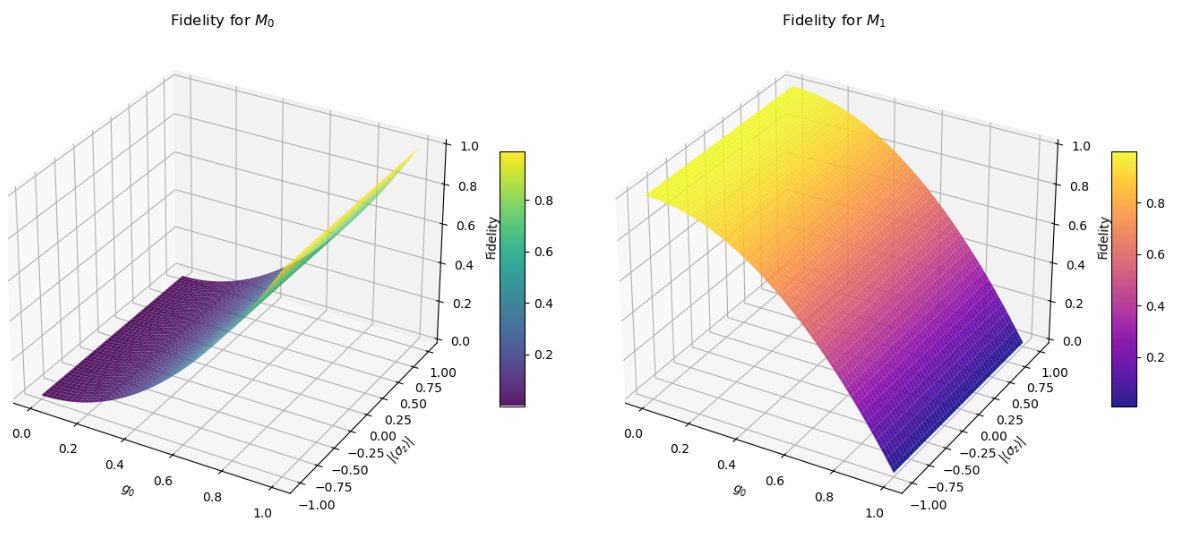
\includegraphics[width=0.9\textwidth]{Fidelity_g0_Sz.png}
	\caption{Fidelity as a function of $ \left| \braket{\sigma_{z}^{j}} \right| $ and $ g_0 $}
	\label{fig:Fidelity_g0_Sz}
\end{figure}
Taking some slices of the 3D plot we see that :
%\graphicspath{ {/home/francesco/Collisional_Methods/Results/Plot/Probability} }
\begin{figure}[H]
	\centering
	% First Pannel(a)
	\begin{subfigure}[b]{0.48\textwidth}
		\centering
		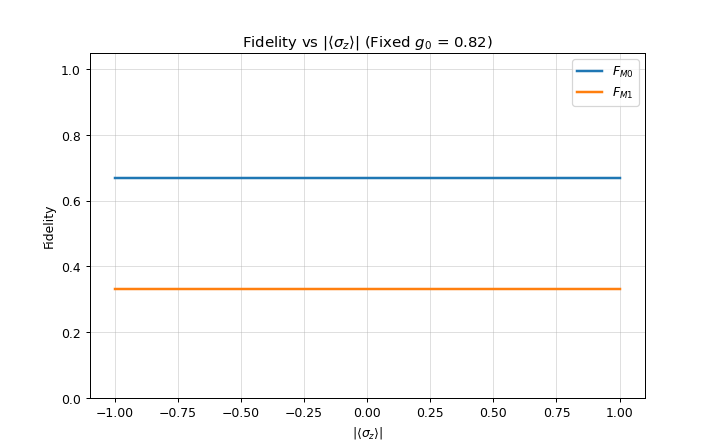
\includegraphics[width=\textwidth]{Fidelity_Sz_1.png}
		\caption{}
		\label{fig:Fidelity_Sz_1}
	\end{subfigure}
	\hfill
	% Second Pannel (b)
	\begin{subfigure}[b]{0.48\textwidth}
		\centering
		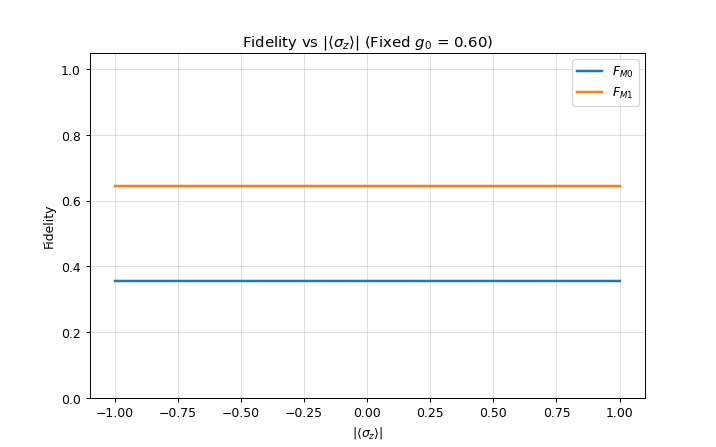
\includegraphics[width=\textwidth]{Fidelity_Sz_2.png}
		\caption{}
		\label{fig:Fidelity_Sz_2}
	\end{subfigure}

	\caption{Fidelity as a function of only $\left| \braket{\sigma_{z}^{j}} \right|$ for different values of $g_0$. Panel (a) shows the results for $ g_{0} = 0.82 $, while panel (b) displays the outcome for $ g_{0} = 0.60 $.}
	\label{fig:Fidelity_Sz}
\end{figure}

This plots gives confirmation of the fact that the second term proportional to $\left| \braket{\sigma_{z}^{j}} \right|$ it's negligible, in fact we have the same results for different value of $\left| \braket{\sigma_{z}^{j}} \right|$ in Fig.\ref{fig:Fidelity_g0} and there's no quadratic dependence on $\left| \braket{\sigma_{z}^{j}} \right|$ in Fig.\ref{fig:Fidelity_Sz}, where the Fidelity essentially are constants equal to :
\begin{gather}
	\mathcal{F}_{\mathcal{M}_{0}} \approx g_{0}^{2} \cos^{2}\left(c_{j} \Delta t \right) \\
	\mathcal{F}_{\mathcal{M}_{1}} \approx \left(1 - g_{0}^{2}\right) \cos^{2}\left(c_{j} \Delta t \right)
\end{gather}

Another important thing to check is the distribution of $\left| \braket{\sigma_{z}^{j}} \right|$ and $\left| \braket{\sigma_{z}^{j}} \right|^2$ recorded during the dynamics for different \textit{Unraveling Scheme}. With this results we should see if different unraveling gives different values of the quantities described above, i.e. some states are more visited or one site is more populated during the trajectories. This could directly affect the fidelity, which also depends, and in a practically irrelevant way, on $\left| \braket{\sigma_{z}^{j}} \right|$ which in turn depends on the sampled state at each time step (for example, eigenstates of $ \sigma_{z} $ would have $ \mathcal{F} = 1 $, i.e. rotation around the z-axis is irrelevant).

At this purpose for every Trajectory and at every time step the values of $\left| \braket{\sigma_{z}^{1}} \right|$ and $\left| \braket{\sigma_{z}^{2}} \right|$ were calculated and stored in two matrices \texttt{Sz\_matrix\_1(n\_times, N\_traj)} and \texttt{Sz\_matrix\_2(n\_times, N\_traj)}; notice that :
\begin{gather}
	 \braket{\sigma_{z}^{1}} = \bra{\Psi_{S}} \sigma_{z}^{1} \ket{\Psi_{S}} \quad \text{where} \quad \sigma_{z}^{1} = \sigma_{z} \otimes \mathbb{I} \\
	 \braket{\sigma_{z}^{2}} = \bra{\Psi_{S}} \sigma_{z}^{2} \ket{\Psi_{S}} \quad \text{where} \quad \sigma_{z}^{2} = \mathbb{I} \otimes \sigma_{z}
\end{gather}

Once we've obtained \texttt{Sz\_matrix\_1(n\_times, N\_traj)} and \texttt{Sz\_matrix\_2(n\_times, N\_traj)}, it's possible to calculate the average value over the trajectories and then the square values, that enter in Eq.\ref{eq:fidelity_M0} and Eq.\ref{eq:fidelity_M1}. Finally, the temporal distribution of these results was visualized using histograms :

%\graphicspath{ {/home/francesco/Collisional\_Methods/Results/Plot/Sxyz\_exp\_value/Distribution} }
\begin{figure}[H]
	\centering
	% First Panel(a)
	\begin{subfigure}[b]{0.48\textwidth}
		\centering
		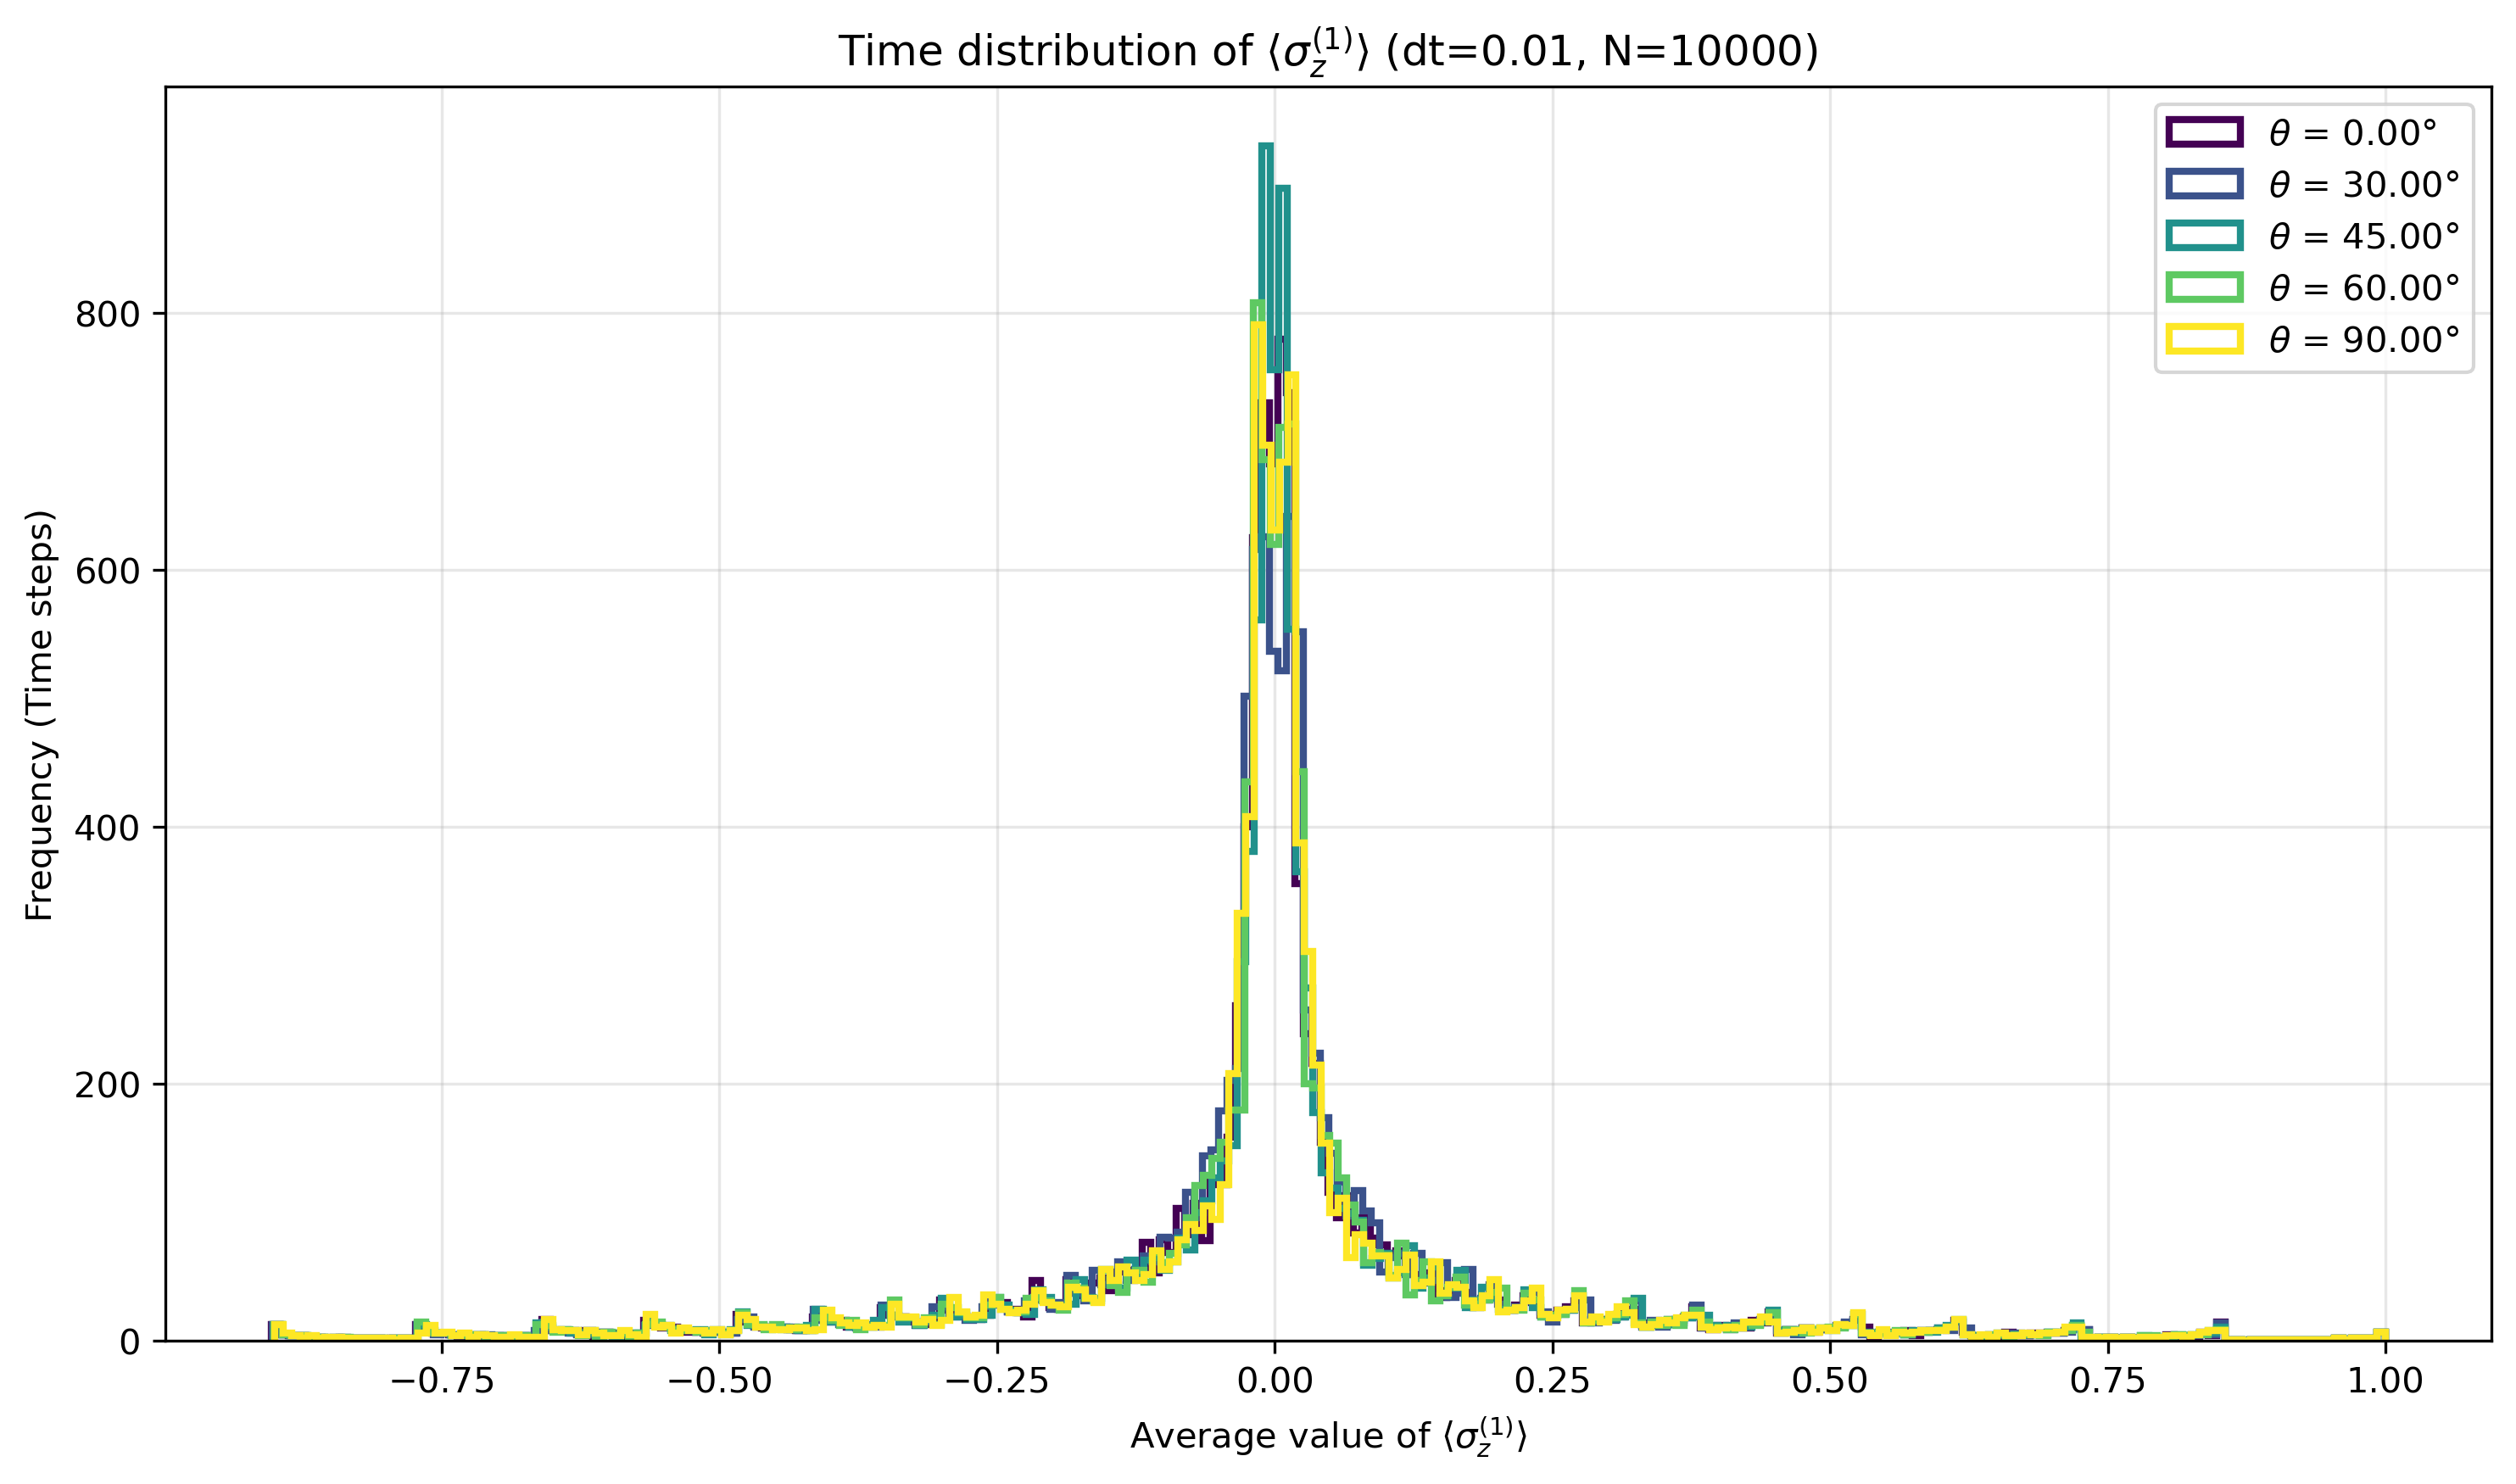
\includegraphics[width=\textwidth]{Sz_distribution_intermediate.png}
		\caption{}
		\label{fig:Sz_avg}
	\end{subfigure}
	\hfill
	% Second Panel(b)
	\begin{subfigure}[b]{0.48\textwidth}
		\centering
		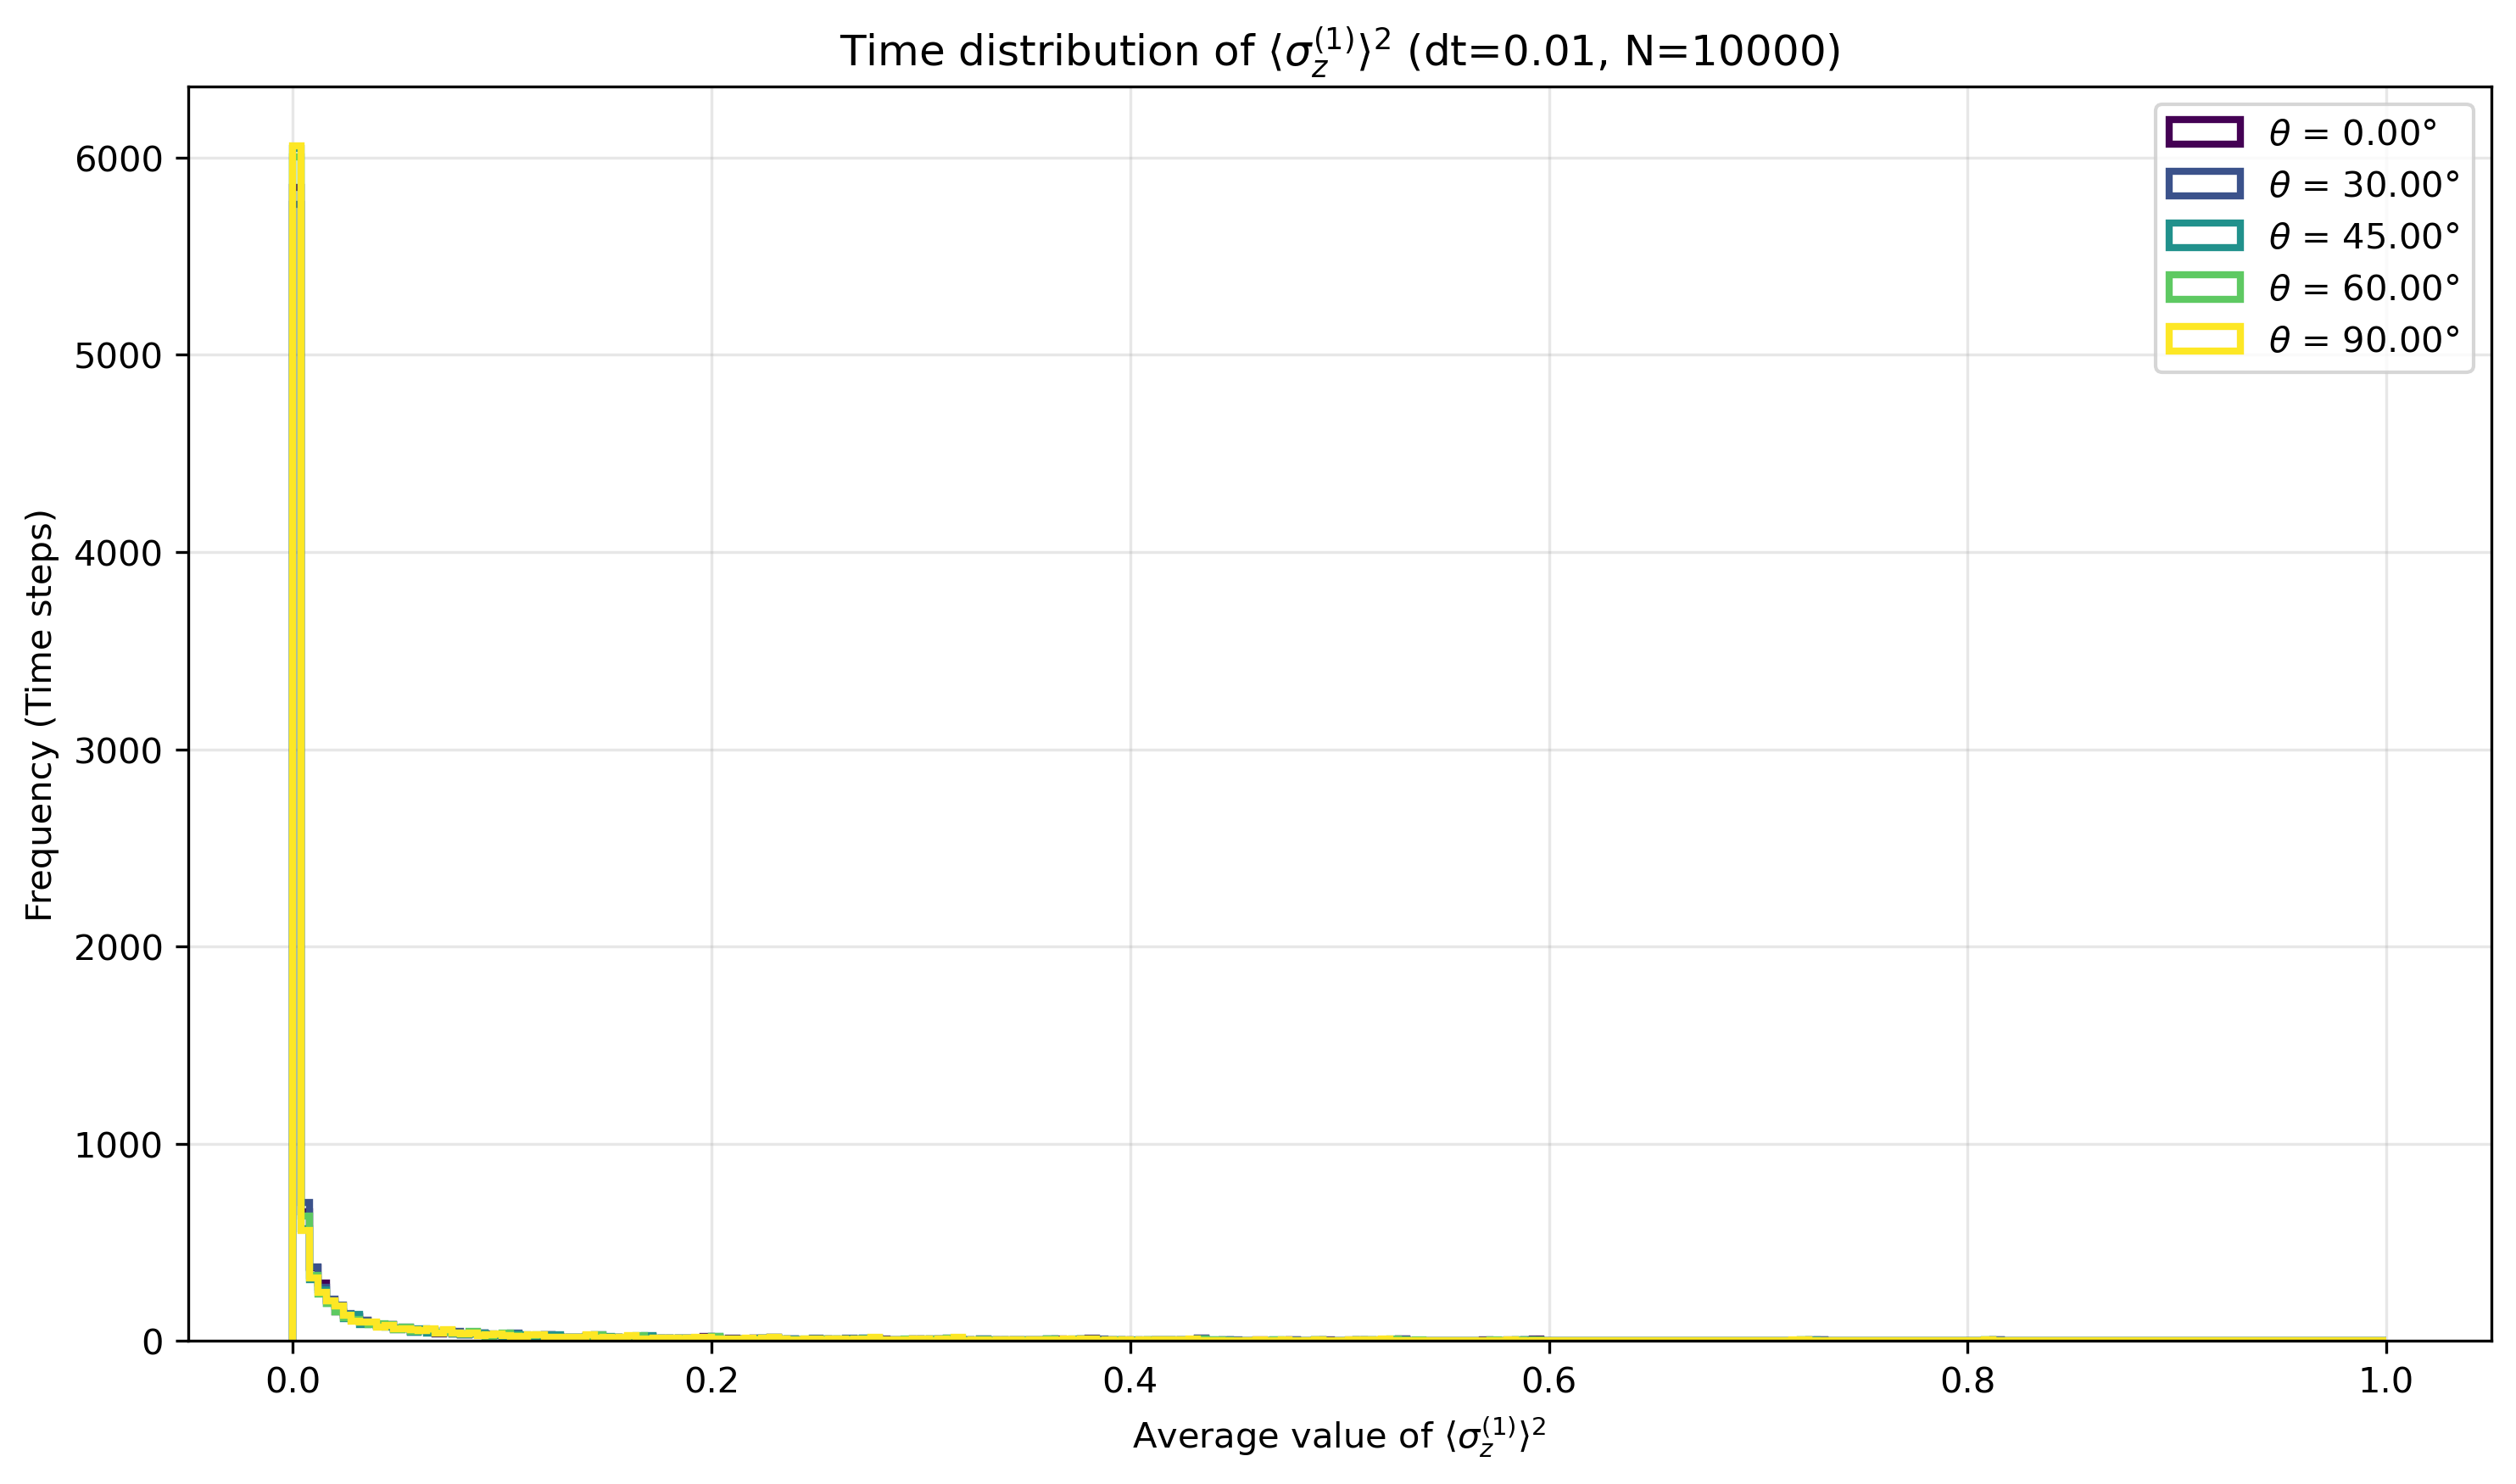
\includegraphics[width=\textwidth]{Sz_square_distribution_intermediate.png}
		\caption{}
		\label{fig:Sz_square_avg}
	\end{subfigure}
	\caption{Distribution of $\left| \braket{\sigma_{z}^{1}} \right|$ in panel (a), and $\left| \braket{\sigma_{z}^{1}} \right|^2$ in panel (b), recorded during the dynamics and averaged over 10,000 trajectories.}
	\label{fig:Sz_distributions}
\end{figure}

\begin{figure}[H]
	\centering
	% First Panel(a)
	\begin{subfigure}[b]{0.48\textwidth}
		\centering
		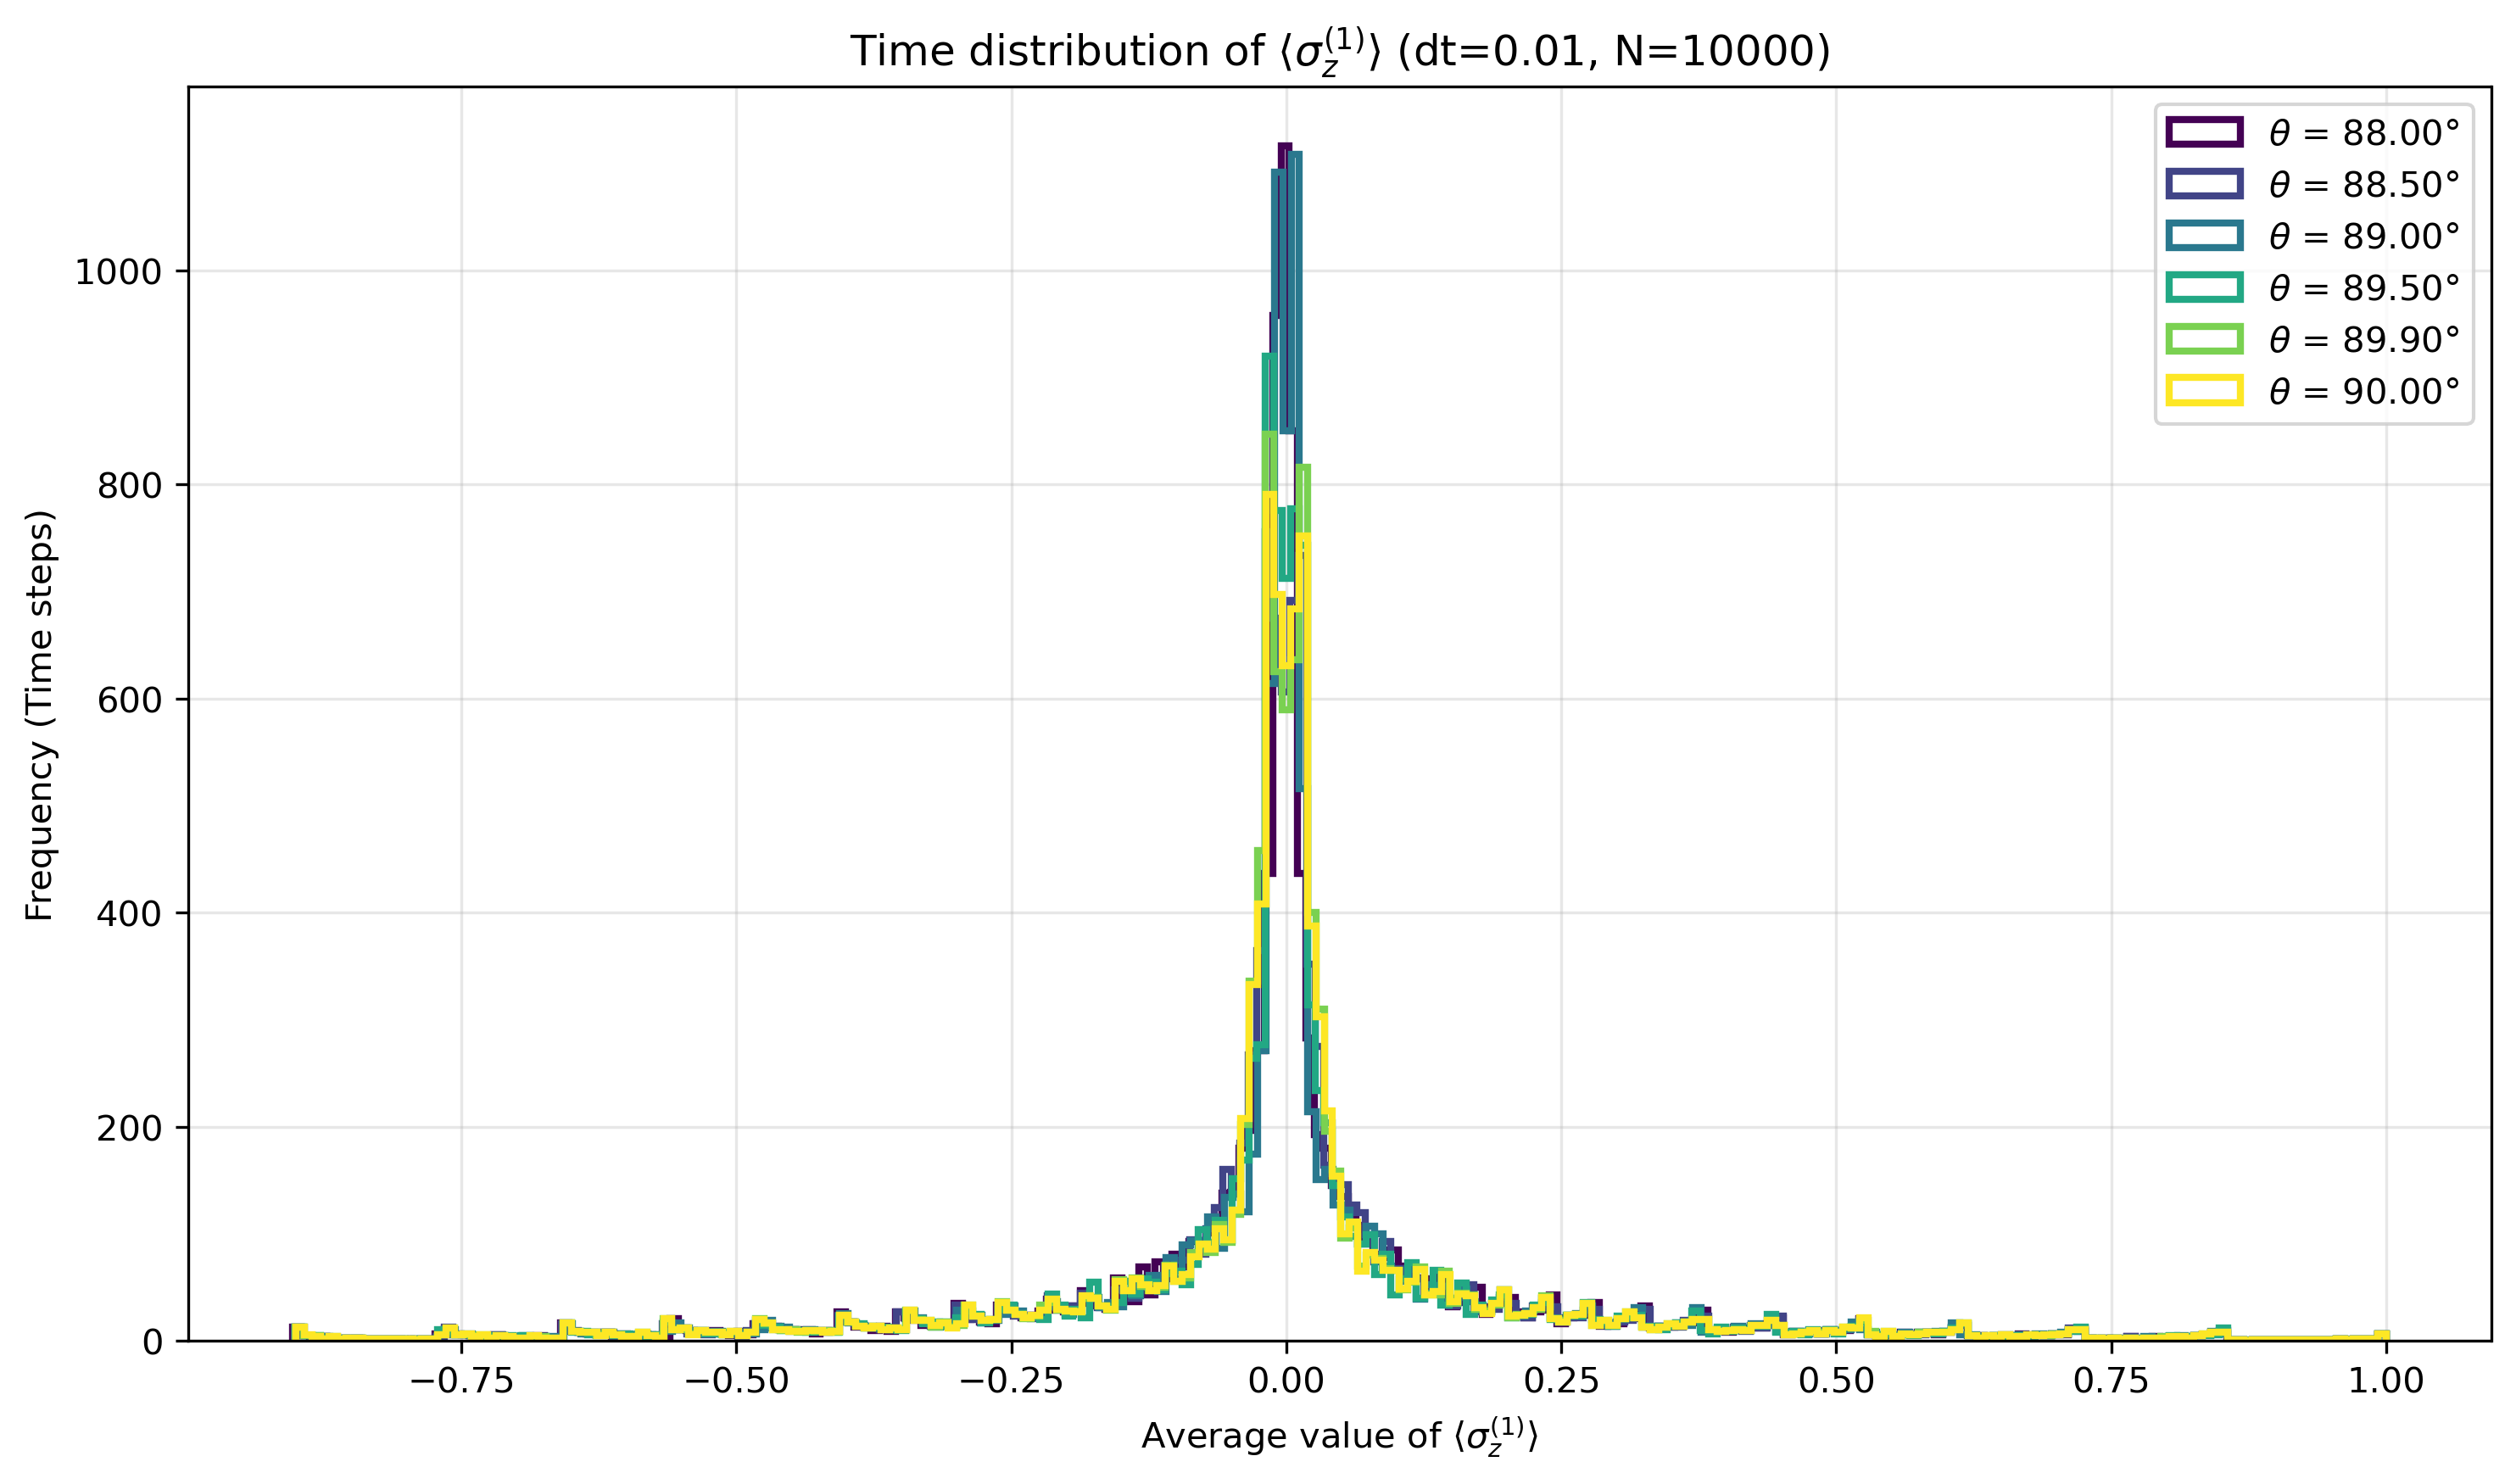
\includegraphics[width=\textwidth]{Sz_distribution_close_to_90_deg.png}
		\caption{}
		\label{fig:Sz_avg_close_to_90}
	\end{subfigure}
	\hfill
	% Second Panel(b)
	\begin{subfigure}[b]{0.48\textwidth}
		\centering
		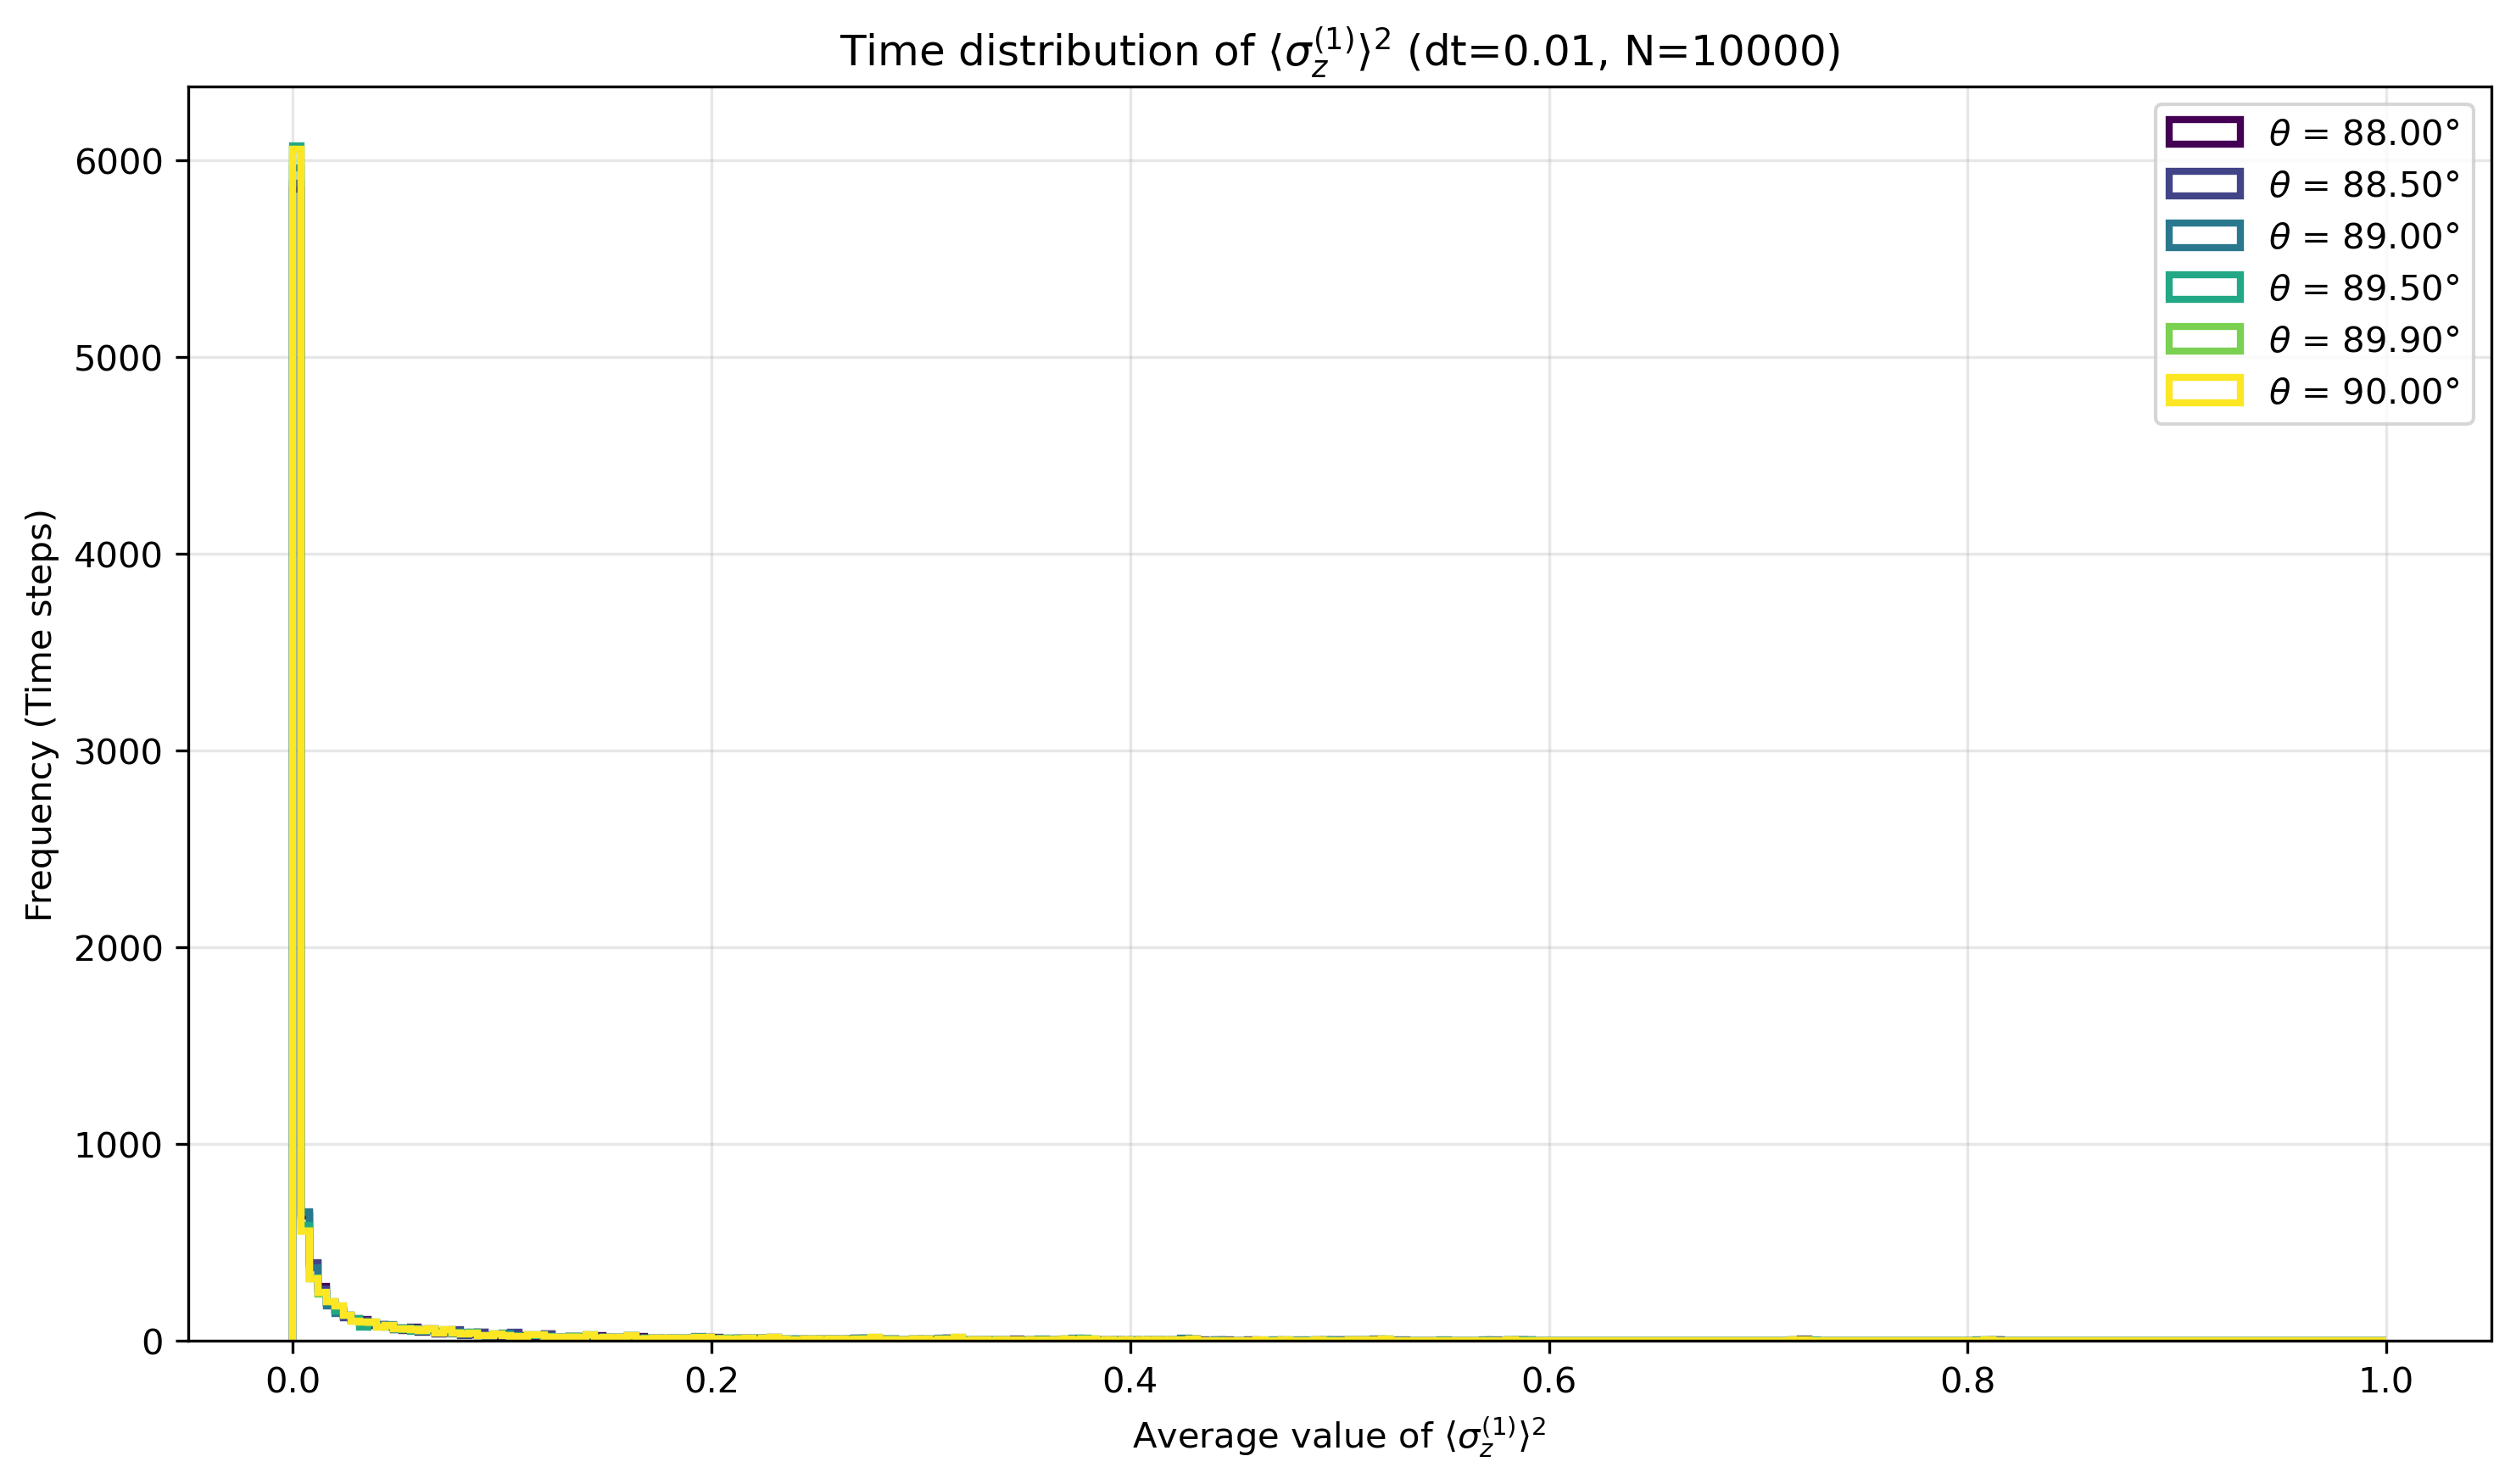
\includegraphics[width=\textwidth]{Sz_square_distribution_close_to_90_deg.png}
		\caption{}
		\label{fig:Sz_square_avg_close_to_90}
	\end{subfigure}
	\caption{Distribution of $\left| \braket{\sigma_{z}^{1}} \right|$ in panel (a), and $\left| \braket{\sigma_{z}^{1}} \right|^2$ in panel (b), recorded during the dynamics and averaged over 10,000 trajectories, for angles close to 90°.}
	\label{fig:Sz_distributions_close_to_90_deg}
\end{figure}

As expected the histograms give the same distribution for different unraveling scheme, which is centered in 0.0, since the \textit{Ensamble Average}, over the trajectories, reproduces the Lindblad distribution of $ \braket{\sigma_{z}^{j}} $, so since the dynamics of the site populatin is a dumped oscillation towards the value 0.5 and $ \braket{\sigma_{z}^{j}} \propto P_{10} - P_{01} $, values close to 0.0 should be sampled more often. Consequentially the squared values are just the squared positive part of the $ \braket{\sigma_{z}^{j}} $ distribution.

Notice that only $ \braket{\sigma_{z}^{j}} $ is calculated since this value i related to the single site, where in the \textit{Dephasing Dynamics} where only the excited states are populated, $ \braket{\sigma_{x}^{j}} = \braket{\sigma_{y}^{j}} = 0 $. \\

\newpage

As seen before the fidelity calculated in Eq.\ref{eq:fidelity_M0} and Eq.\ref{eq:fidelity_M1} are referred to the variation induced by the collision with a single site. If we want to calculate the fidelity referred to the total variation of the system $ \ket{\Psi}_{S} = c_{00} \ket{0_{1}0_{2}} + c_{10} \ket{1_{1}0_{2}} + c_{01} \ket{0_{1}1_{2}} + c_{11} \ket{1_{1}1_{2}} $ (considering the \textit{entanglement}) we have to work with $ \mathcal{M}_{\alpha, \beta} $, so that, since we are always working with pure states, the \textit{Fidelity} becomes:
\begin{align}
	\mathcal{F}_{\mathcal{M}_{00}} &= \left| \braket{\Psi_{S}^{PRE} | \Psi_{S}^{POST}}_{\mathcal{M}_{00}} \right|^2 = \left| \bra{\Psi_{S}^{PRE}}\mathcal{M}_{00} \ket{\Psi_{S}^{PRE}} \right|^2 \notag \\
	&= \left[ g_0^2 \cos(c_1 \Delta t) \cos(c_2 \Delta t) - g_1^2 \sin(c_1 \Delta t) \sin(c_2 \Delta t) \braket{\sigma_z \otimes \sigma_z} \right]^2 \notag \\
	&\quad + g_0^2 g_1^2 \left[ \sin(c_1 \Delta t) \cos(c_2 \Delta t) \braket{\sigma_z^1} + \cos(c_1 \Delta t) \sin(c_2 \Delta t) \braket{\sigma_z^2} \right]^2 \label{eq:fidelity_M00_general} \\
	\mathcal{F}_{\mathcal{M}_{10}} &= \left| \braket{\Psi_{S}^{PRE} | \Psi_{S}^{POST}}_{\mathcal{M}_{10}} \right|^2 = \left| \bra{\Psi_{S}^{PRE}}\mathcal{M}_{10} \ket{\Psi_{S}^{PRE}} \right|^2 \notag \\
	&= g_0^2 g_1^2 \left[ \cos(c_1 \Delta t) \cos(c_2 \Delta t) + \sin(c_1 \Delta t) \sin(c_2 \Delta t) \braket{\sigma_z \otimes \sigma_z} \right]^2 \notag \\
	&\quad + \left[ g_0^2 \sin(c_1 \Delta t) \cos(c_2 \Delta t) \braket{\sigma_z^1} - g_1^2 \cos(c_1 \Delta t) \sin(c_2 \Delta t) \braket{\sigma_z^2} \right]^2 \label{eq:fidelity_M10_general} \\
	\mathcal{F}_{\mathcal{M}_{01}} &= \left| \braket{\Psi_{S}^{PRE} | \Psi_{S}^{POST}}_{\mathcal{M}_{01}} \right|^2 = \left| \bra{\Psi_{S}^{PRE}}\mathcal{M}_{01} \ket{\Psi_{S}^{PRE}} \right|^2 \notag \\
	&= g_0^2 g_1^2 \left[ \cos(c_1 \Delta t) \cos(c_2 \Delta t) + \sin(c_1 \Delta t) \sin(c_2 \Delta t) \braket{\sigma_z \otimes \sigma_z} \right]^2 \notag \\
	&\quad + \left[ g_1^2 \sin(c_1 \Delta t) \cos(c_2 \Delta t) \braket{\sigma_z^1} - g_0^2 \cos(c_1 \Delta t) \sin(c_2 \Delta t) \braket{\sigma_z^2} \right]^2 \label{eq:fidelity_M01_general} \\
	\mathcal{F}_{\mathcal{M}_{11}} &= \left| \braket{\Psi_{S}^{PRE} | \Psi_{S}^{POST}}_{\mathcal{M}_{11}} \right|^2 = \left| \bra{\Psi_{S}^{PRE}}\mathcal{M}_{11} \ket{\Psi_{S}^{PRE}} \right|^2 \notag \\
	&= \left[ g_1^2 \cos(c_1 \Delta t) \cos(c_2 \Delta t) - g_0^2 \sin(c_1 \Delta t) \sin(c_2 \Delta t) \braket{\sigma_z \otimes \sigma_z} \right]^2 \notag \\
	&\quad + g_0^2 g_1^2 \left[ \sin(c_1 \Delta t) \cos(c_2 \Delta t) \braket{\sigma_z^1} + \cos(c_1 \Delta t) \sin(c_2 \Delta t) \braket{\sigma_z^2} \right]^2 \label{eq:fidelity_M11_general}
\end{align}
Assuming $ c_1 = c_2 $ and in the \textit{Single Exciton Subspace}:
\begin{align}
	\mathcal{F}_{\mathcal{M}_{00}} &= \left| \braket{\Psi_{S}^{PRE} | \Psi_{S}^{POST}}_{\mathcal{M}_{00}} \right|^2 = \left| \bra{\Psi_{S}^{PRE}}\mathcal{M}_{00} \ket{\Psi_{S}^{PRE}} \right|^2 \notag \\
	&= \left[g_0^2 \cos^2{\left(c \Delta t \right)} + g_1^2 \sin^2{\left(c \Delta t \right)}\right]^{2} \label{eq:fidelity_M00} \\
	\mathcal{F}_{\mathcal{M}_{10}} &= \left| \braket{\Psi_{S}^{PRE} | \Psi_{S}^{POST}}_{\mathcal{M}_{10}} \right|^2 = \left| \bra{\Psi_{S}^{PRE}}\mathcal{M}_{10} \ket{\Psi_{S}^{PRE}} \right|^2 \notag \\
	&= g_0^2 g_1^2 \left[ \cos^2(c \Delta t) - \sin^2(c \Delta t) \right]^2 + \sin^2(c \Delta t) \cos^2(c \Delta t) \left| \braket{\sigma_{z}^{1}} \right|^2 \label{eq:fidelity_M10} \\
	\mathcal{F}_{\mathcal{M}_{01}} &= \left| \braket{\Psi_{S}^{PRE} | \Psi_{S}^{POST}}_{\mathcal{M}_{01}} \right|^2 = \left| \bra{\Psi_{S}^{PRE}}\mathcal{M}_{01} \ket{\Psi_{S}^{PRE}} \right|^2 \notag \\
	&= g_0^2 g_1^2 \left[ \cos^2(c \Delta t) - \sin^2(c \Delta t) \right]^2 + \sin^2(c \Delta t) \cos^2(c \Delta t) \left| \braket{\sigma_{z}^{1}} \right|^2 \label{eq:fidelity_M01} \\
	\mathcal{F}_{\mathcal{M}_{11}} &= \left| \braket{\Psi_{S}^{PRE} | \Psi_{S}^{POST}}_{\mathcal{M}_{11}} \right|^2 = \left| \bra{\Psi_{S}^{PRE}}\mathcal{M}_{11} \ket{\Psi_{S}^{PRE}} \right|^2 \notag \\
	&= \left[g_1^2 \cos^2{\left(c \Delta t \right)} + g_0^2 \sin^2{\left(c \Delta t \right)} \right]^{2} \label{eq:fidelity_M11}
\end{align}
Notice that $ \mathcal{F}_{\mathcal{M}_{01}} = \mathcal{F}_{\mathcal{M}_{10}} $

\newpage

\subsection{Fidelity, Trace Distance and Variance}
\label{sub:Fidelity_Trace_Distance_Variance}
In this subsection we will analyze the value of some metric used to compare the Density Matrix, at every time step, obtained averaging over a finite number of trajectories with the one obtained with the Lindblad QME. The metrics used in this case are : 
\begin{itemize}
	\item \textbf{Fidelity} : quantifies the "closeness" or indistinguishability between two quantum states, by measuring the overlap of the two; for two general mixed states  described by density operators $ \rho \text{and} \sigma $ is defined as (in the Uhlmann - Jozsa convention ):
	\begin{equation}
		\mathcal{F} \left( \rho, \sigma \right) = \left( Tr\left[ \sqrt{\sqrt{\rho} \sigma \sqrt{\rho}} \right] \right)^{2} 
	\end{equation}
	for two pure states it becomes : 
	\begin{equation}
		\mathcal{F} \left( \rho, \sigma \right) = | \braket{\phi_{\rho} | \psi_{\sigma}} |^{2}
	\end{equation}
	where $ \rho = \ket{\phi_{\rho}}\bra{\phi_{\rho}} $ and $ \sigma = \ket{\psi_{\sigma}}\bra{\psi_{\sigma}} $. \newline
	In the case of a pure state $ \rho $ and a completely mixed one $ \sigma $ the Fidelity takes on the value of $ \mathcal{F} = 0.5 $ \newline
	Formally the Fidelity isn't a correct metric, since it doesn't obey the triangle inequality, so to obtain an effective metric a definition based on the angle between the two states is used : 
	\begin{equation}
		\Theta = \arccos{\left( \sqrt{\mathcal{F} \left( \rho, \sigma \right)} \right)}
	\end{equation}
	
	\item \textbf{Trace Distance} : is a foundational geometric metric, which satisfies all the properties of a true mathematical metric and that provides a strict, operational measure of the absolute distinguishability between two quantum states. \newline
	For two general mixed states  described by density operators $ \rho \text{and} \sigma $ is defined as :
	\begin{equation}
		\mathcal{T} \left( \rho, \sigma \right) = \frac{1}{2} Tr \left[ \sqrt{ \left( \rho - \sigma \right)^{\dagger} \left( \rho - \sigma \right) } \right]
	\end{equation}
	for two pure states becomes :
	\begin{equation}
		\mathcal{T} \left( \rho, \sigma \right) = \sqrt{1 - | \braket{\phi_{\rho} | \psi_{\sigma}} |^{2}}
	\end{equation}
	where $ \rho = \ket{\phi_{\rho}}\bra{\phi_{\rho}} $ and $ \sigma = \ket{\psi_{\sigma}}\bra{\psi_{\sigma}} $. \newline
\end{itemize}    
The \textit{Fuchs - van de Graaf inequality} defines the relation between this two metrics : 
\begin{equation}
	1 - \sqrt{\mathcal{F} \left( \rho, \sigma \right)} \leq \mathcal{T} \left( \rho, \sigma \right) \leq \sqrt{1 - \mathcal{F} \left( \rho, \sigma \right)}
\end{equation}
in the case of two pure states the relationship becomes exact:
\begin{equation}
	\mathcal{T} \left( \rho, \sigma \right)  = \sqrt{1 - \mathcal{F} \left( \rho, \sigma \right) }
\end{equation}
This expression provides a clear geometric intuition: the trace distance yields a value of 1 for completely orthogonal (perfectly distinguishable) states, and 0 for identical states.

\newpage
 
In this study, \textit{Fidelity} and \textit{Trace Distance} are used as a quantifier of the \textbf{Convergence Error} associated with the average over a finite number of trajectories, with respect to the Lindblad dynamics. Indeed, $ \mathcal{T} \left( \rho, \sigma \right) $ and $ 1 - \mathcal{F} \left( \rho, \sigma \right) $ (\textit{Infideliy}) are used to evaluate the distance and the difference between the Density Matrix, at every time, obtained by averaging over the trajectories, $ \sigma^{A} (t) = \frac{1}{N_{Traj}} \sum_{n}^{N_{Traj}}{\ket{\psi_{S}^{n}(t)}\bra{\psi_{S}^{n}(t)}} $ and the one obtained from the Lindbald evolution $ \rho^{L} (t) $, which theoretically corresponds with the average over an infinite number o trajectories.

A first calculation was made to analyze the trend over time of the Trace Distance and the Fidelity, obtained by averaging on a number of trajectories equal to 100, 1000 and 10000; here we report the lot for different value of the $ \theta $ angle, which defines the $ H_{Coll} $ direction (Eq.\ref{eq:gz_gx_geom_def}): 
\begin{figure}[H]
	\centering
	\begin{subfigure}[b]{0.48\textwidth}
		\centering
		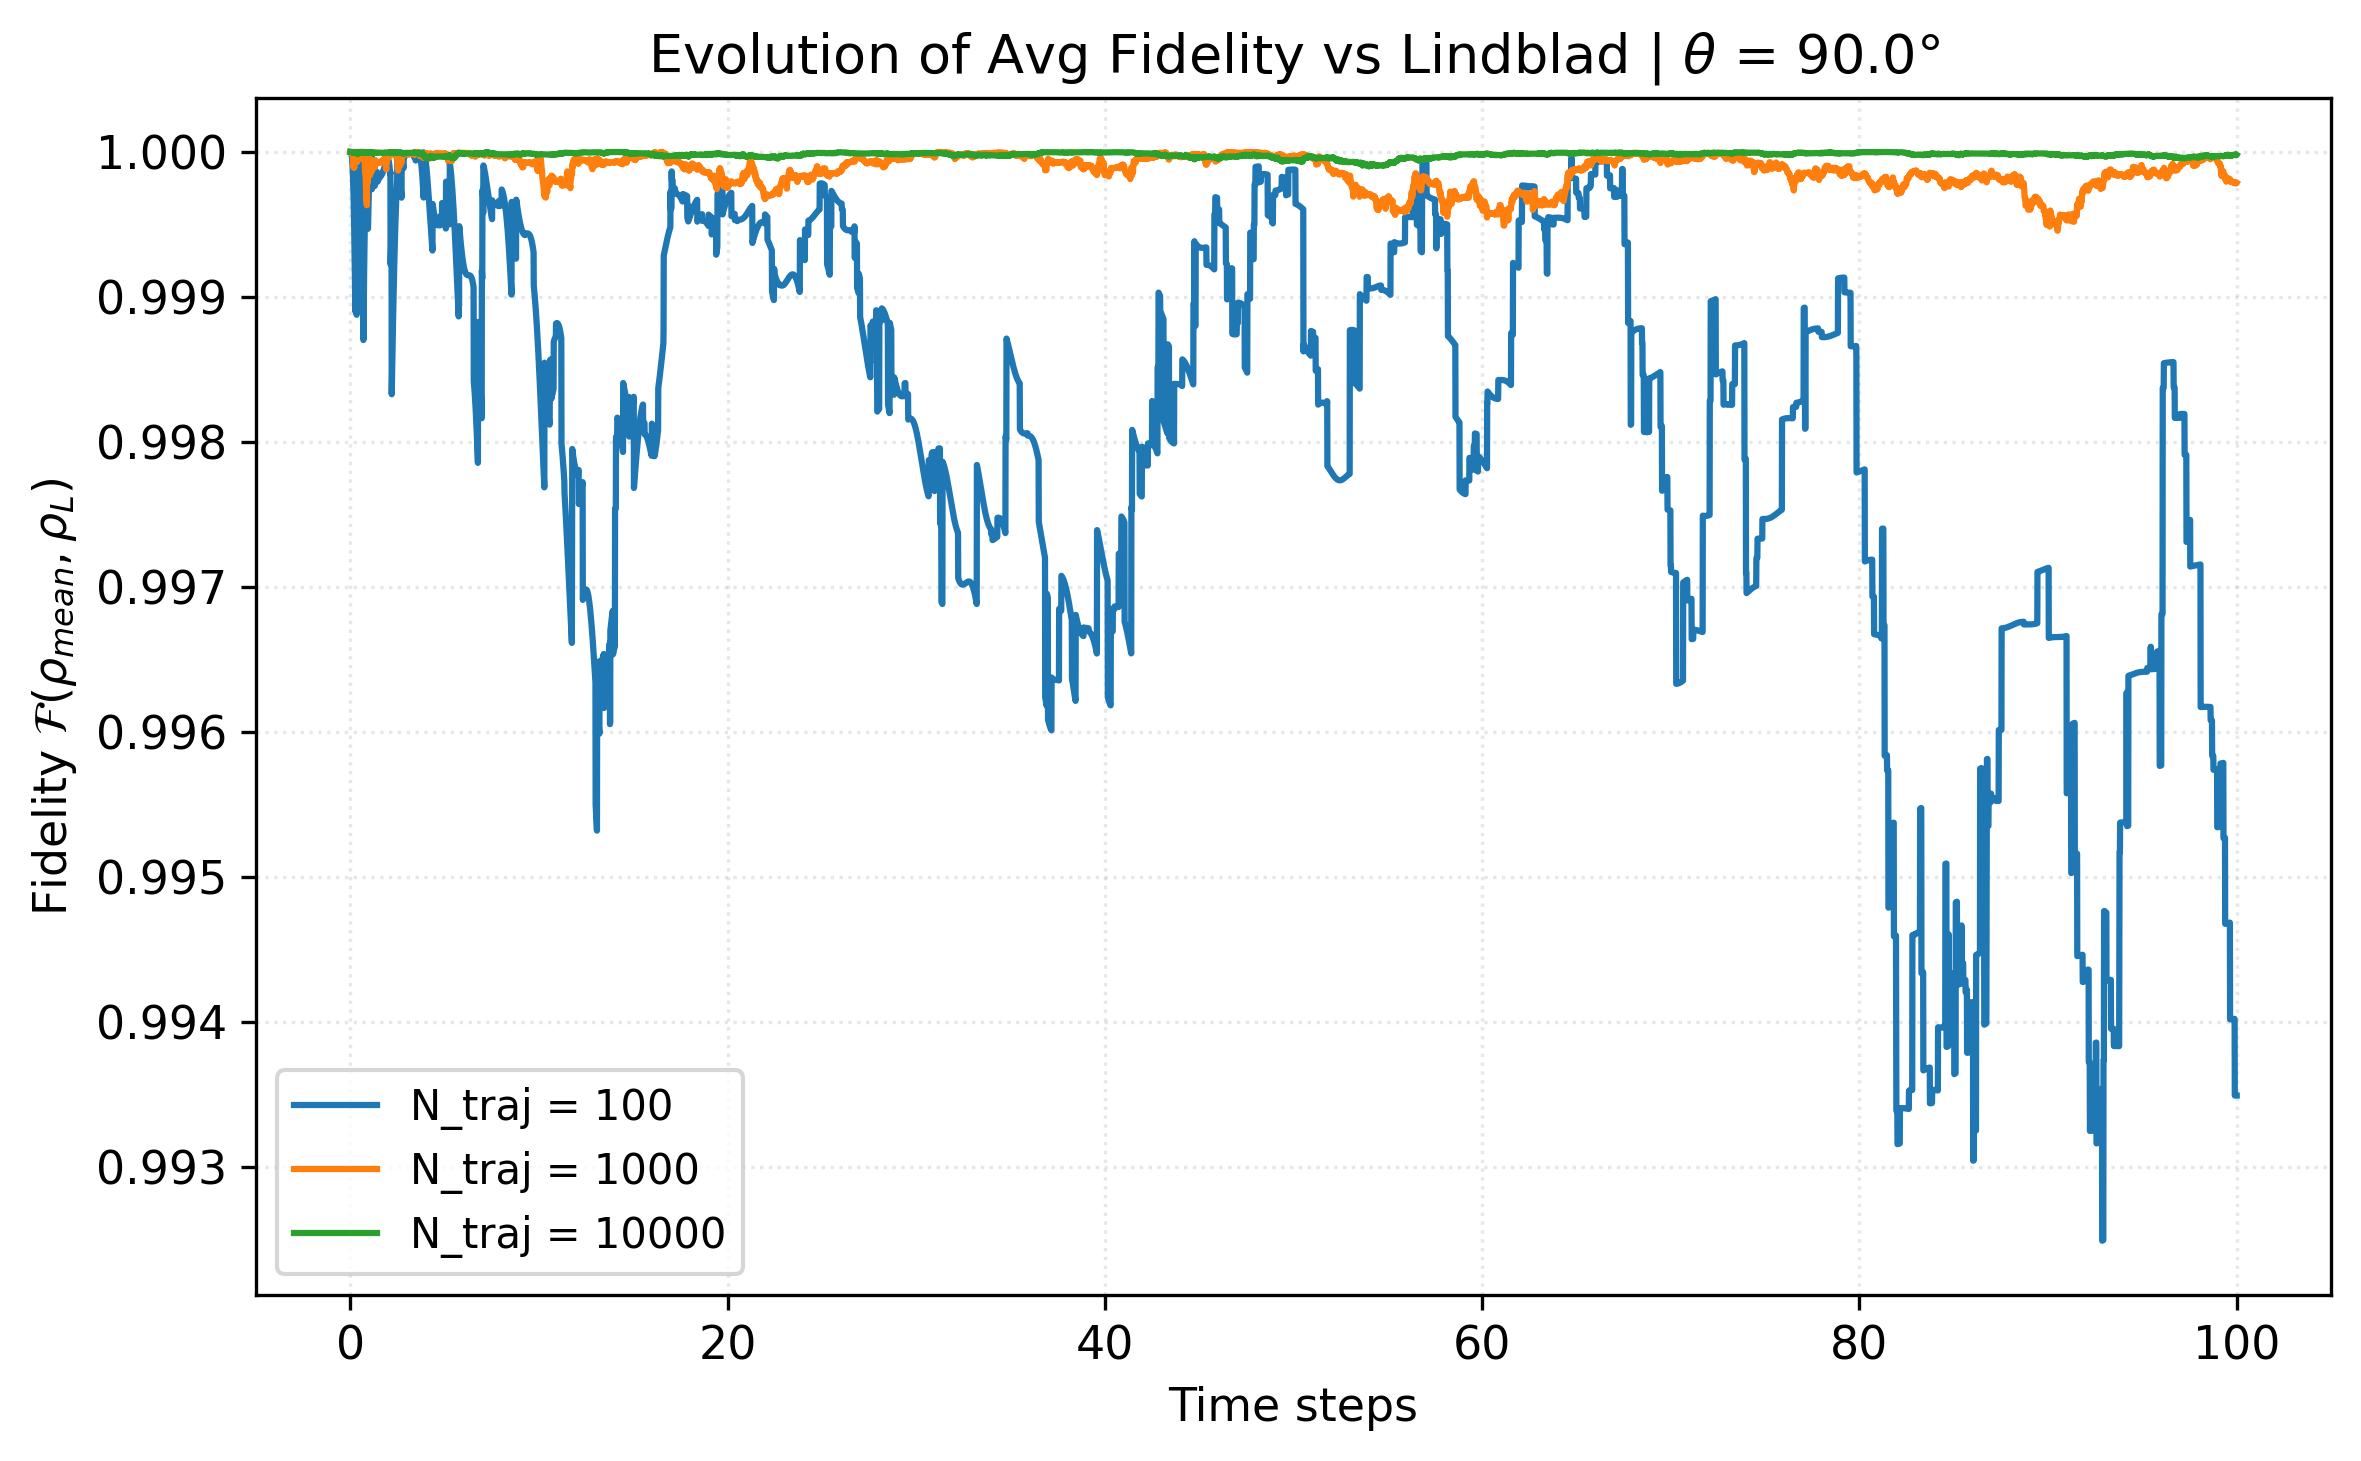
\includegraphics[width=\textwidth]{Avg_Fidelity_Evolution_Theta_1p570796_dt_0p010000.png}
		\label{fig:panel_a_Fidelity_in_time}
		\caption{}
	\end{subfigure}
	\hfill
	\begin{subfigure}[b]{0.48\textwidth}
		\centering
		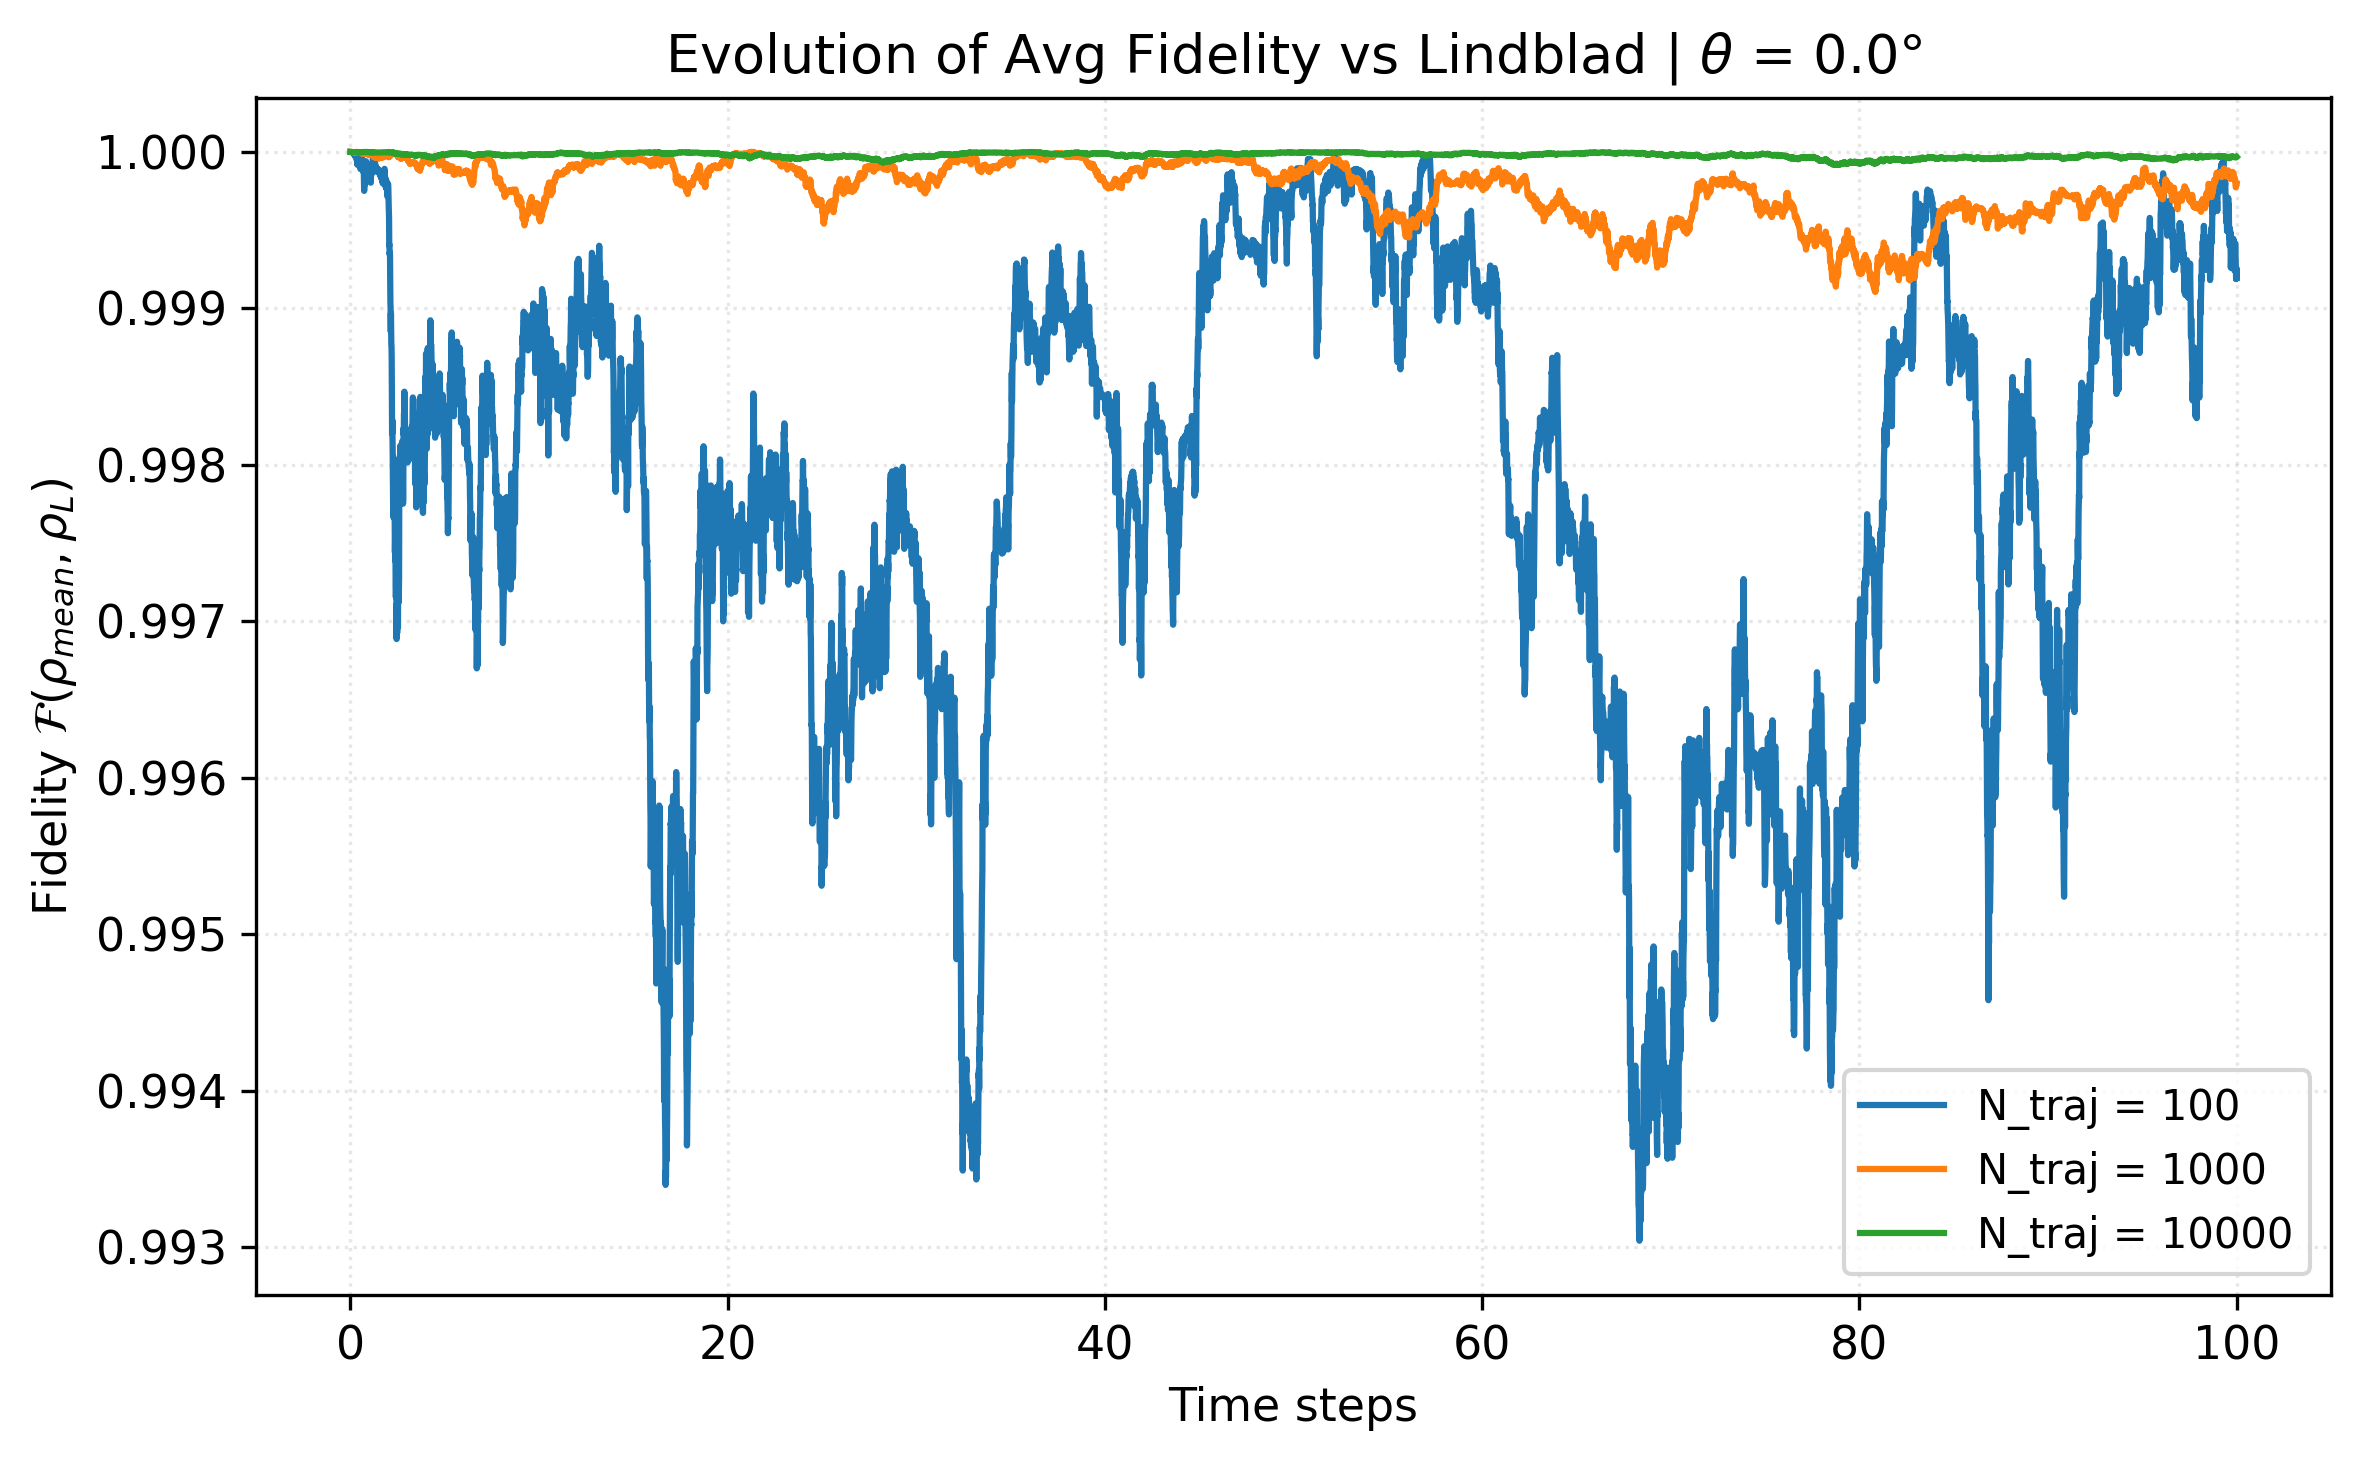
\includegraphics[width=\textwidth]{Avg_Fidelity_Evolution_Theta_0p000000_dt_0p010000.png}
		\label{fig:panel_b_Fidelity_in_time}
		\caption{}
	\end{subfigure}
	\caption{Fidelity in time between $ \sigma^{A} $,  density matrix obtained by averaging over a different number of trajectories, and the Lindbald one $ \rho^{L} $, for a) $ \theta = 90.0^{\circ} $ Quantum Jump Limit and b) $ \theta = 0.0^{\circ} $ State Diffusion Limit. }
\end{figure}
As we could see for both the limit the difference decreases as the number of trajectories increases, reaching a nearly fixed value of 1 per 10,000 trajectories; the oscillation observed for the 100 trajectories are associated with error due to average over a low number of sampling. In both the cases represented the lowest value is approximately the same and still it is relatively close to 1 even with a low number of trajectories.

What could be more informative is the calculation of the Average in Time ( $ \langle \mathcal{F} \left( \rho^{L}, \sigma^{A} \right) \rangle_{t} $, $ \langle \mathcal{T} \left( \rho^{L}, \sigma^{A} \right) \rangle_{t} $ ) and Minimum Value ($ \mathcal{F} \left( \rho^{L}, \sigma^{A} \right)_{Min} $, $ \mathcal{T} \left( \rho^{L}, \sigma^{A} \right)_{Min} $ )of the the two metrics, for different number of trajectories. 
Plotting the values against the $ N_{Traj} $ value, in a log - log scale and fitting them can give information on the \textit{Finite Sampling Convergence Properties} of the Collisional Algorithm; in the following figures we are plotting the value defined before for different $ \theta $ angles : 
\begin{figure}[H]
	\centering
	\begin{subfigure}[b]{0.48\textwidth}
		\centering
		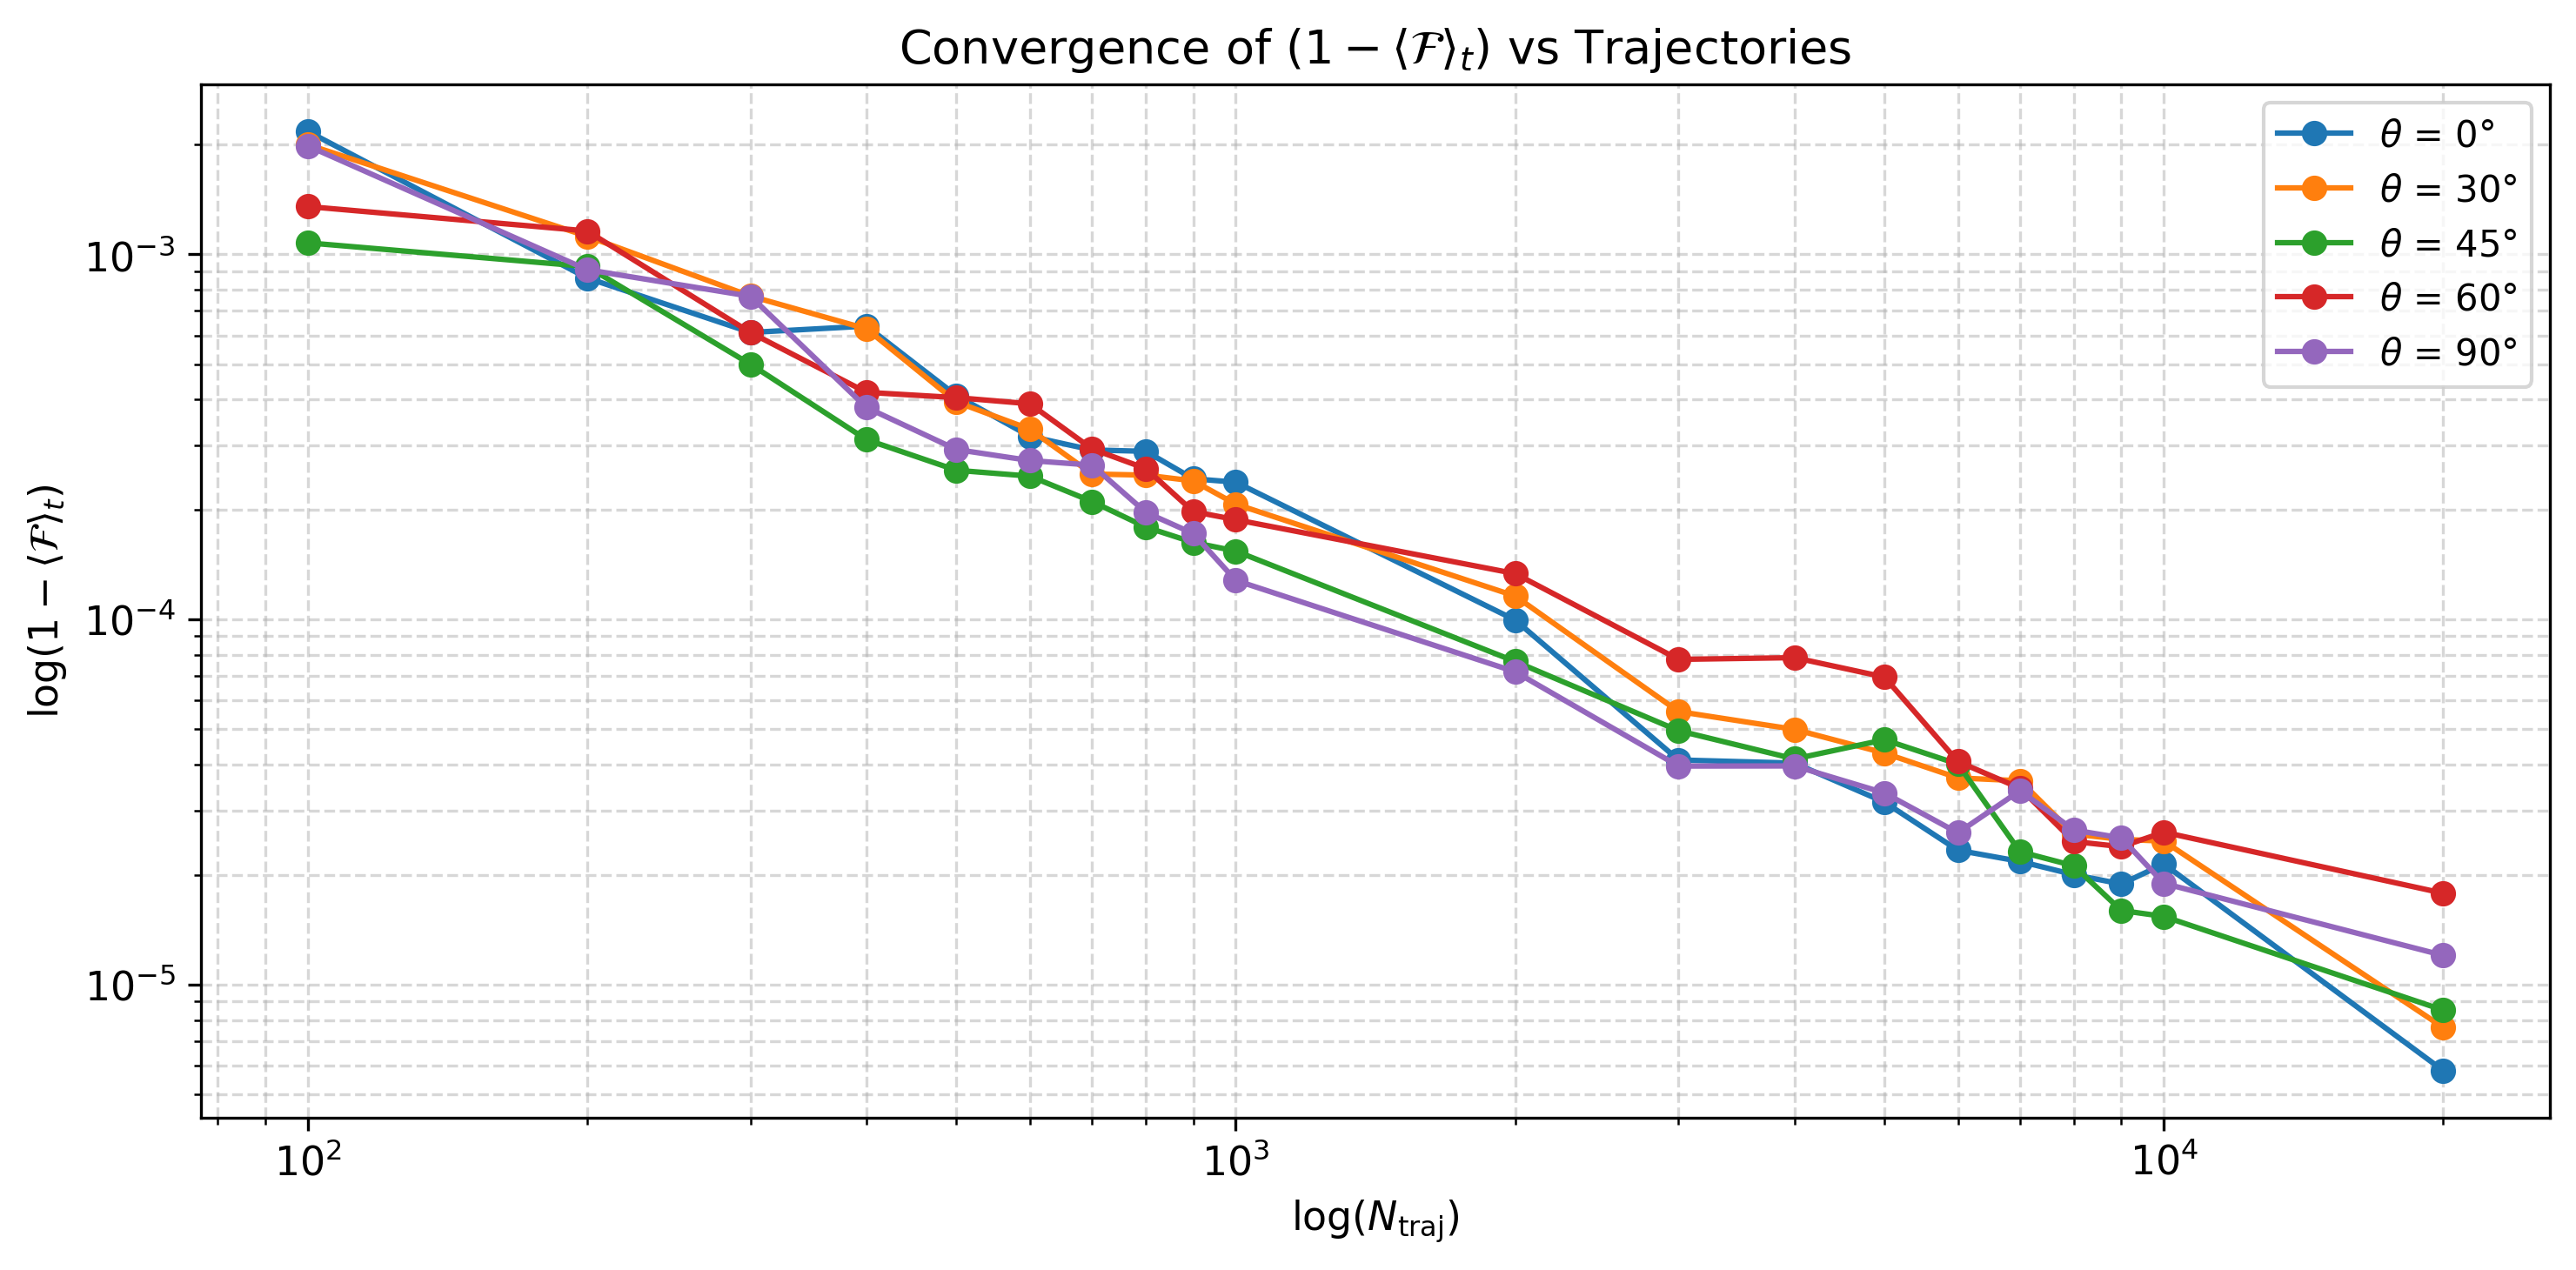
\includegraphics[width=\textwidth]{Avg_Infidelity_in_time_normal.png}
		\label{fig:panel_a_Avg_InFidelity_in_time}
		\caption{}
	\end{subfigure}
	\hfill
	\begin{subfigure}[b]{0.48\textwidth}
		\centering
		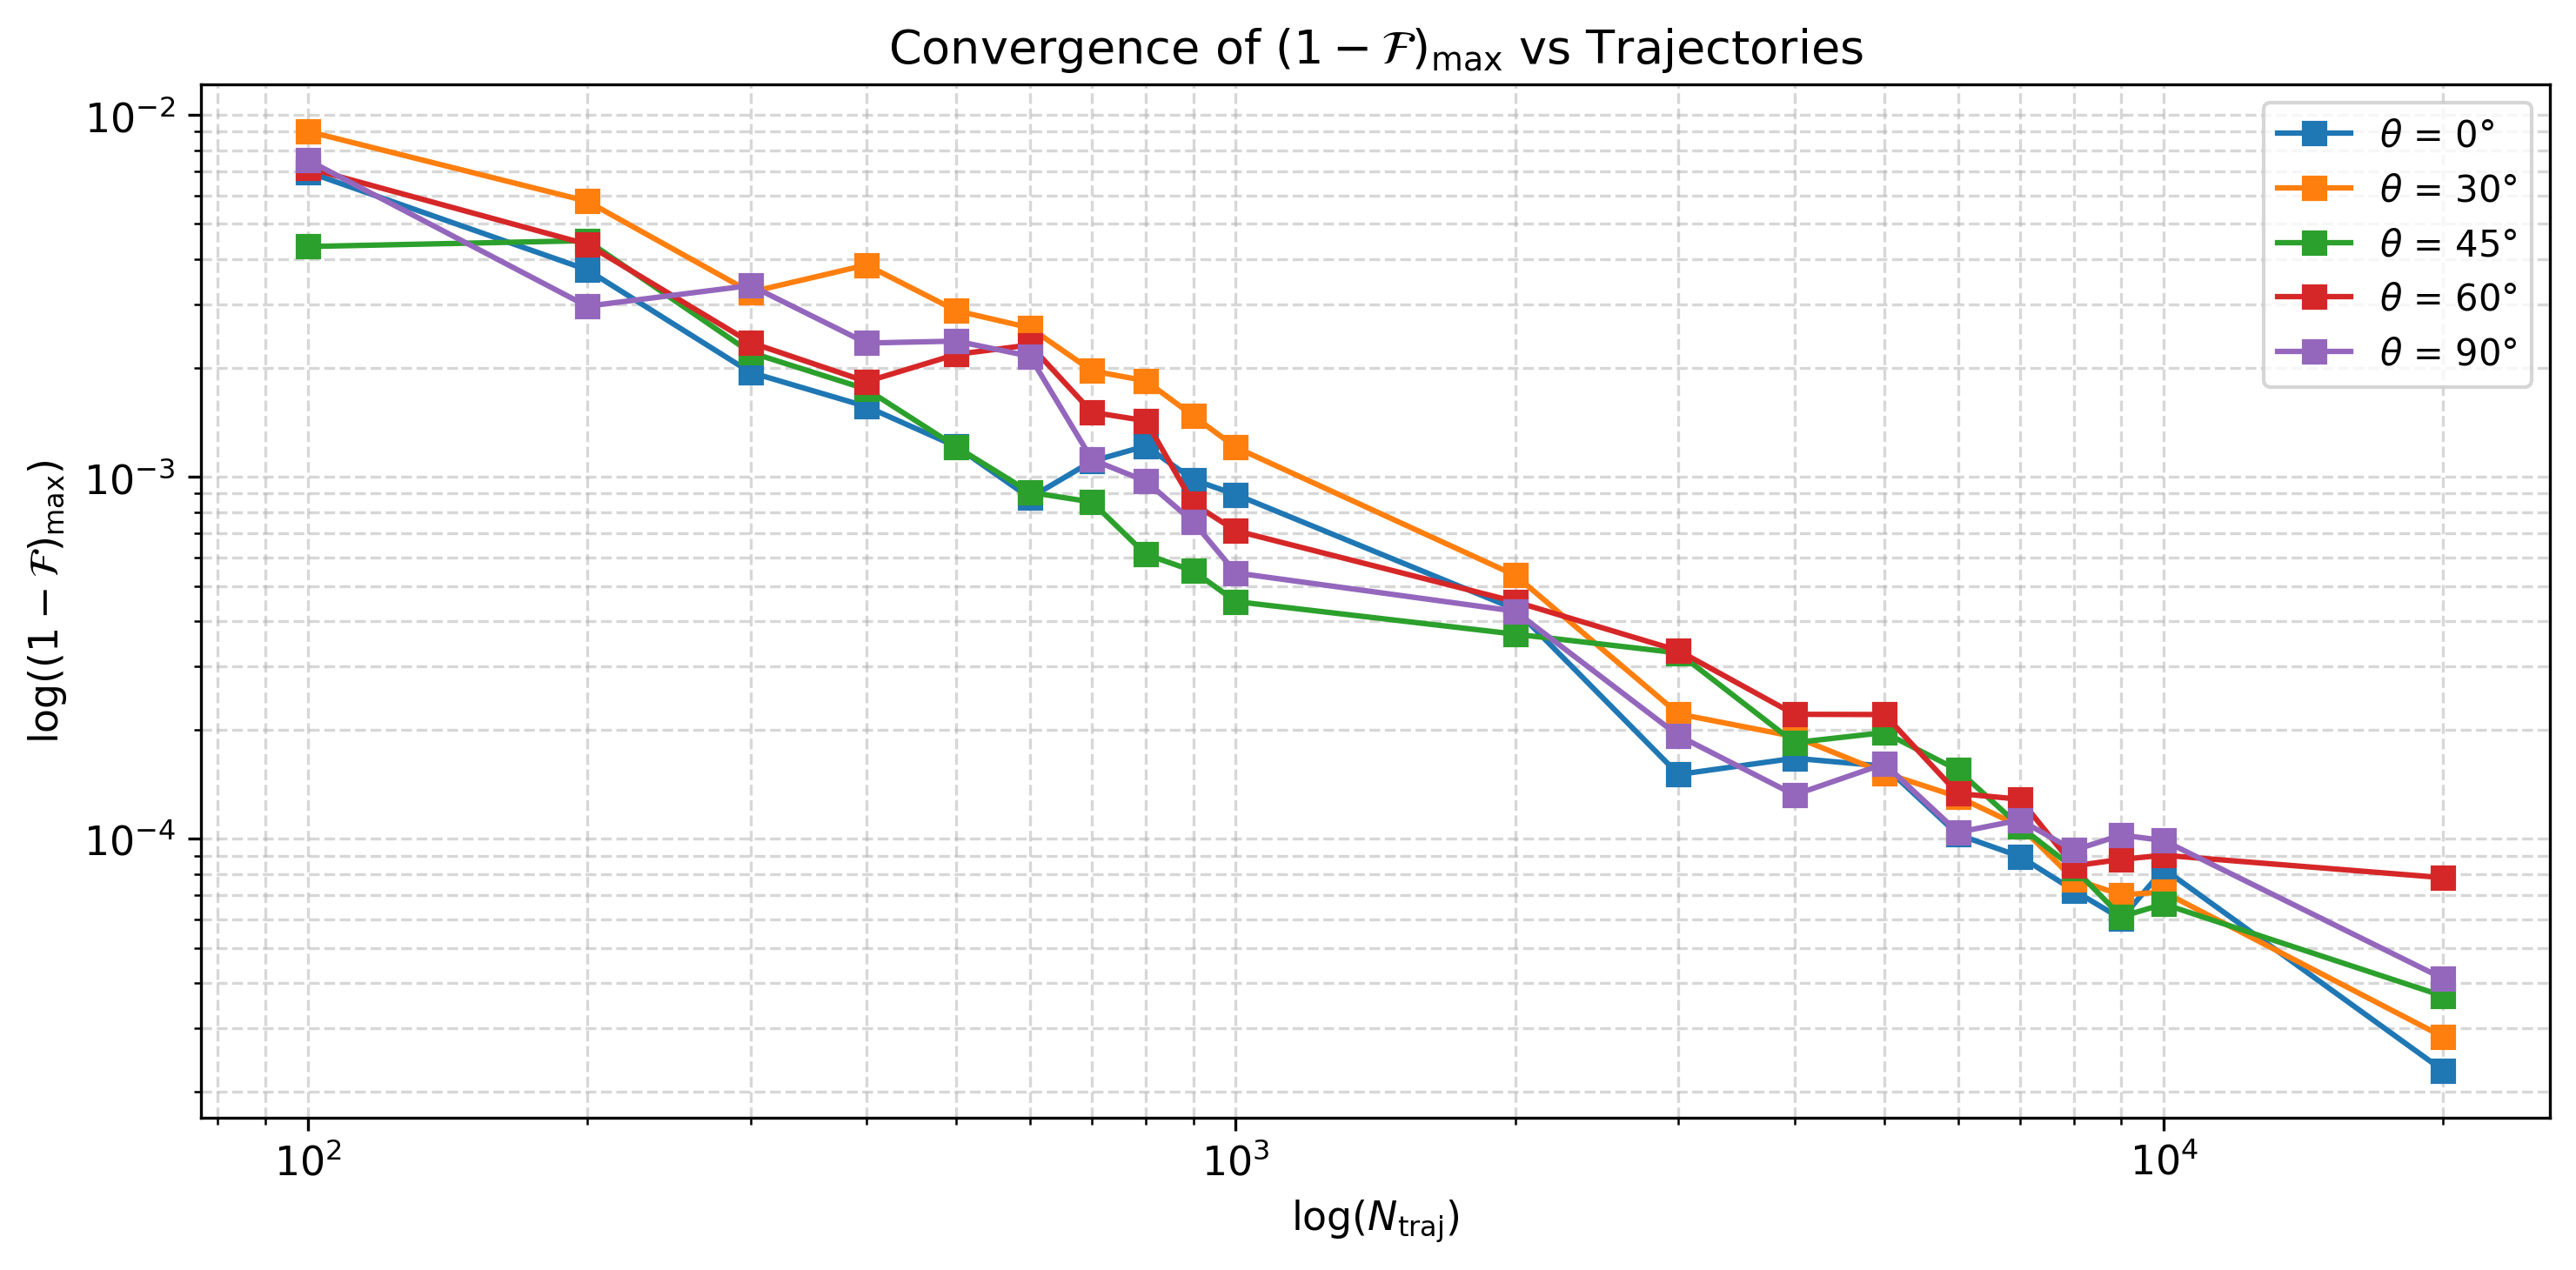
\includegraphics[width=\textwidth]{Max_Infidelity_normal.png}
		\label{fig:panel_b_Max_InFidelity}
		\caption{}
	\end{subfigure}
	\caption{a) Average Value in time and b) Max Value of Infidelity between $ \sigma^{A} $,  density matrix obtained by averaging over a different number of trajectories, and the Lindbald one $ \rho^{L} $, for different value of $ \theta $. }
\end{figure}
METTERE BARRE DI ERRORE !!!!!!!!
\begin{figure}[H]
	\centering
	\begin{subfigure}[b]{0.48\textwidth}
		\centering
		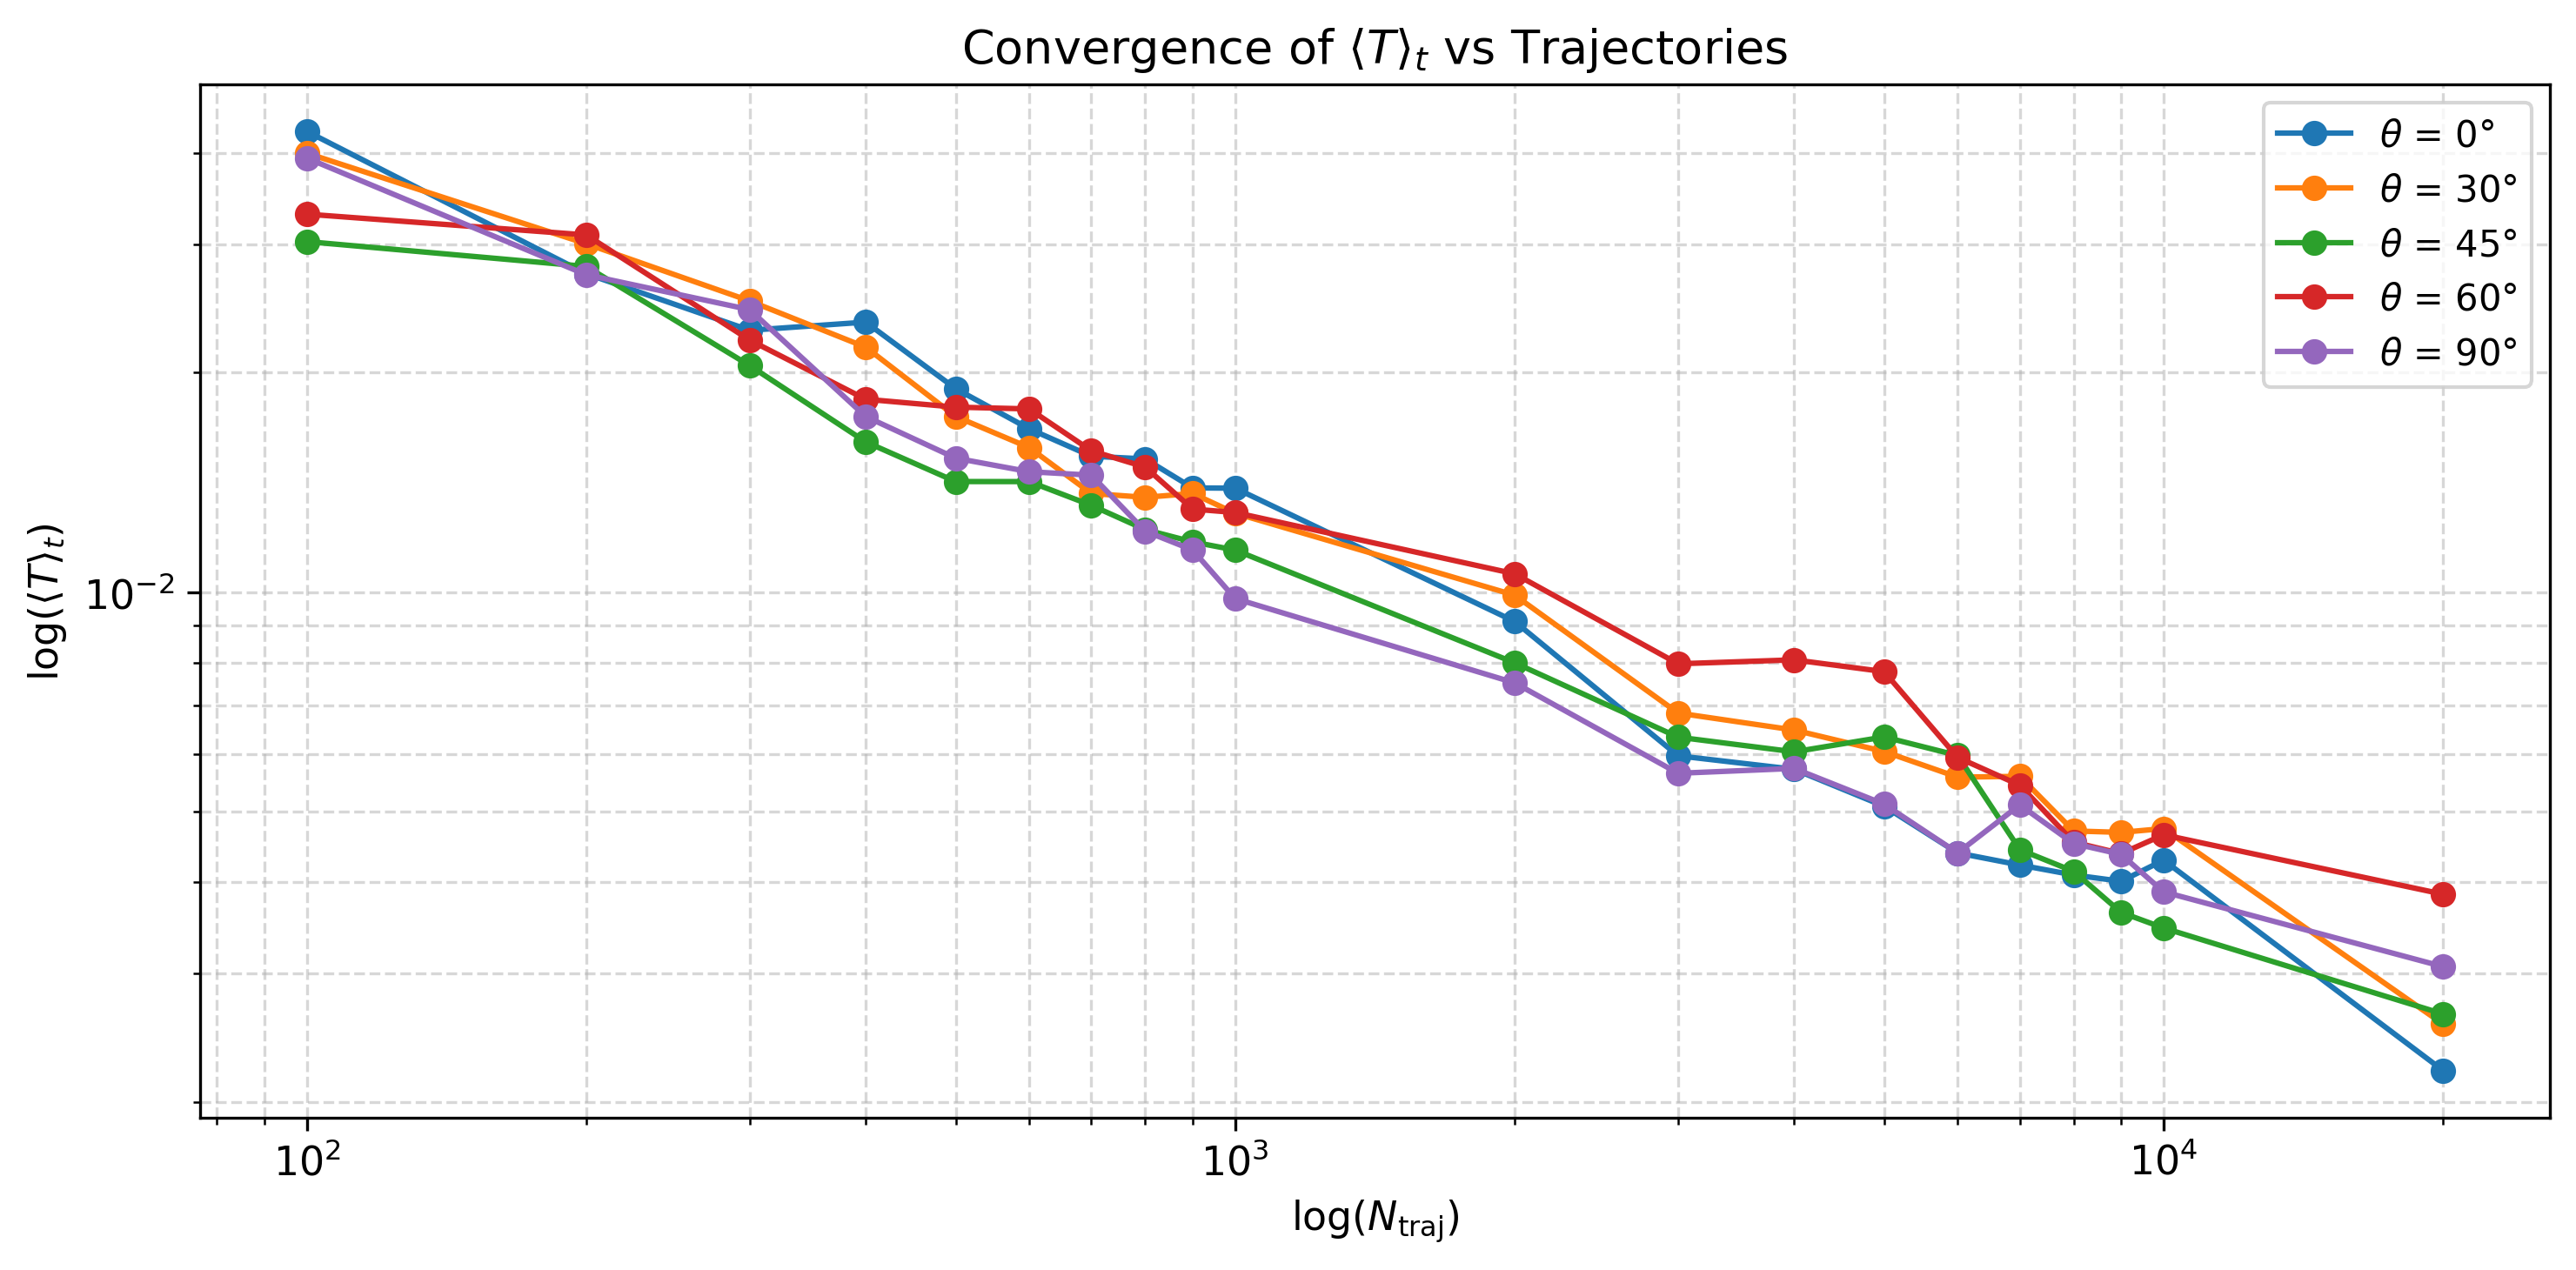
\includegraphics[width=\textwidth]{Avg_Trace_Distance_in_time_normal.png}
		\label{fig:panel_a_Avg_Trace_Distance_in_time}
		\caption{}
	\end{subfigure}
	\hfill
	\begin{subfigure}[b]{0.48\textwidth}
		\centering
		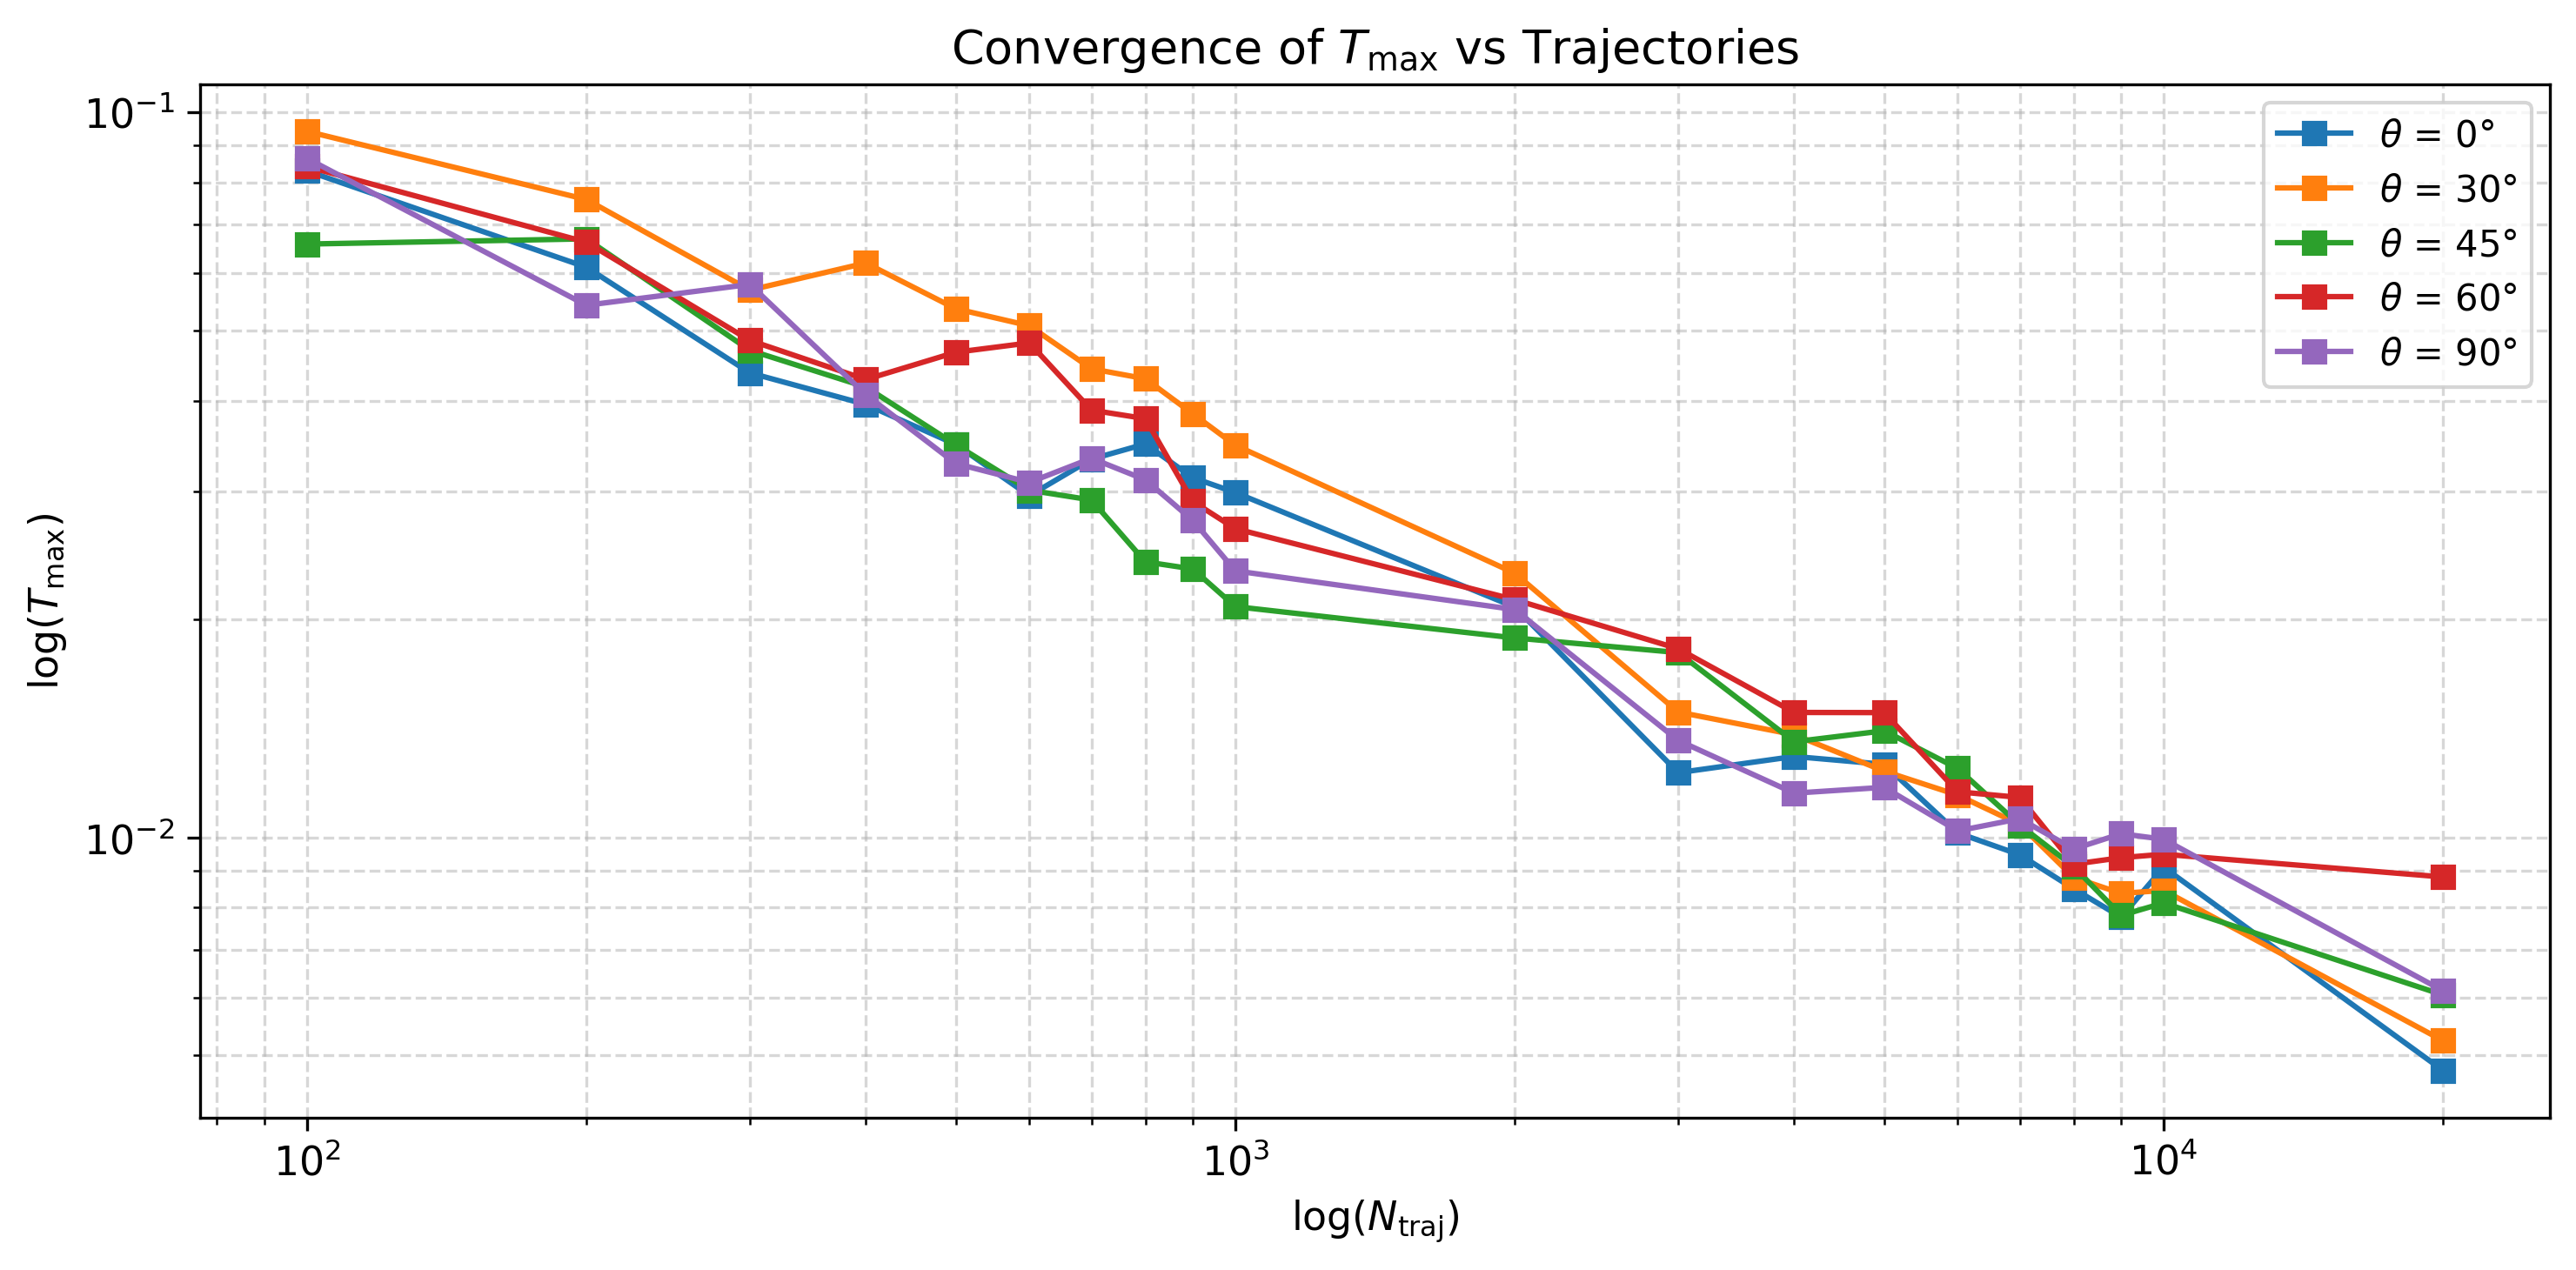
\includegraphics[width=\textwidth]{Max_Trace_Distance_normal.png}
		\label{fig:panel_b_Max_Trace_Distance}
		\caption{}
	\end{subfigure}
	\caption{a) Average Value in time and b) Max Value of Trace Distance between $ \sigma^{A} $,  density matrix obtained by averaging over a different number of trajectories, and the Lindbald one $ \rho^{L} $, for different value of $ \theta $. }
\end{figure}
Since the absolute values are very small and taking into account the errors, what we can state is that there is no substantial difference between the various unraveling scheme, i.e different $ \theta $ angles, as regards the " closure " of the $ \sigma^{A} $ and $ \rho^{L} $.   
By performing a Linear Fitting of the values obtained it's possible to define the trend of convergence with respect to $ _{Traj} $; in this case the analysis was performed only for the mean trace distance values $ \langle \mathcal{T} \left( \rho^{L}, \sigma^{A} \right) \rangle_{t}  $ : 
\begin{figure}[H]
	\centering
	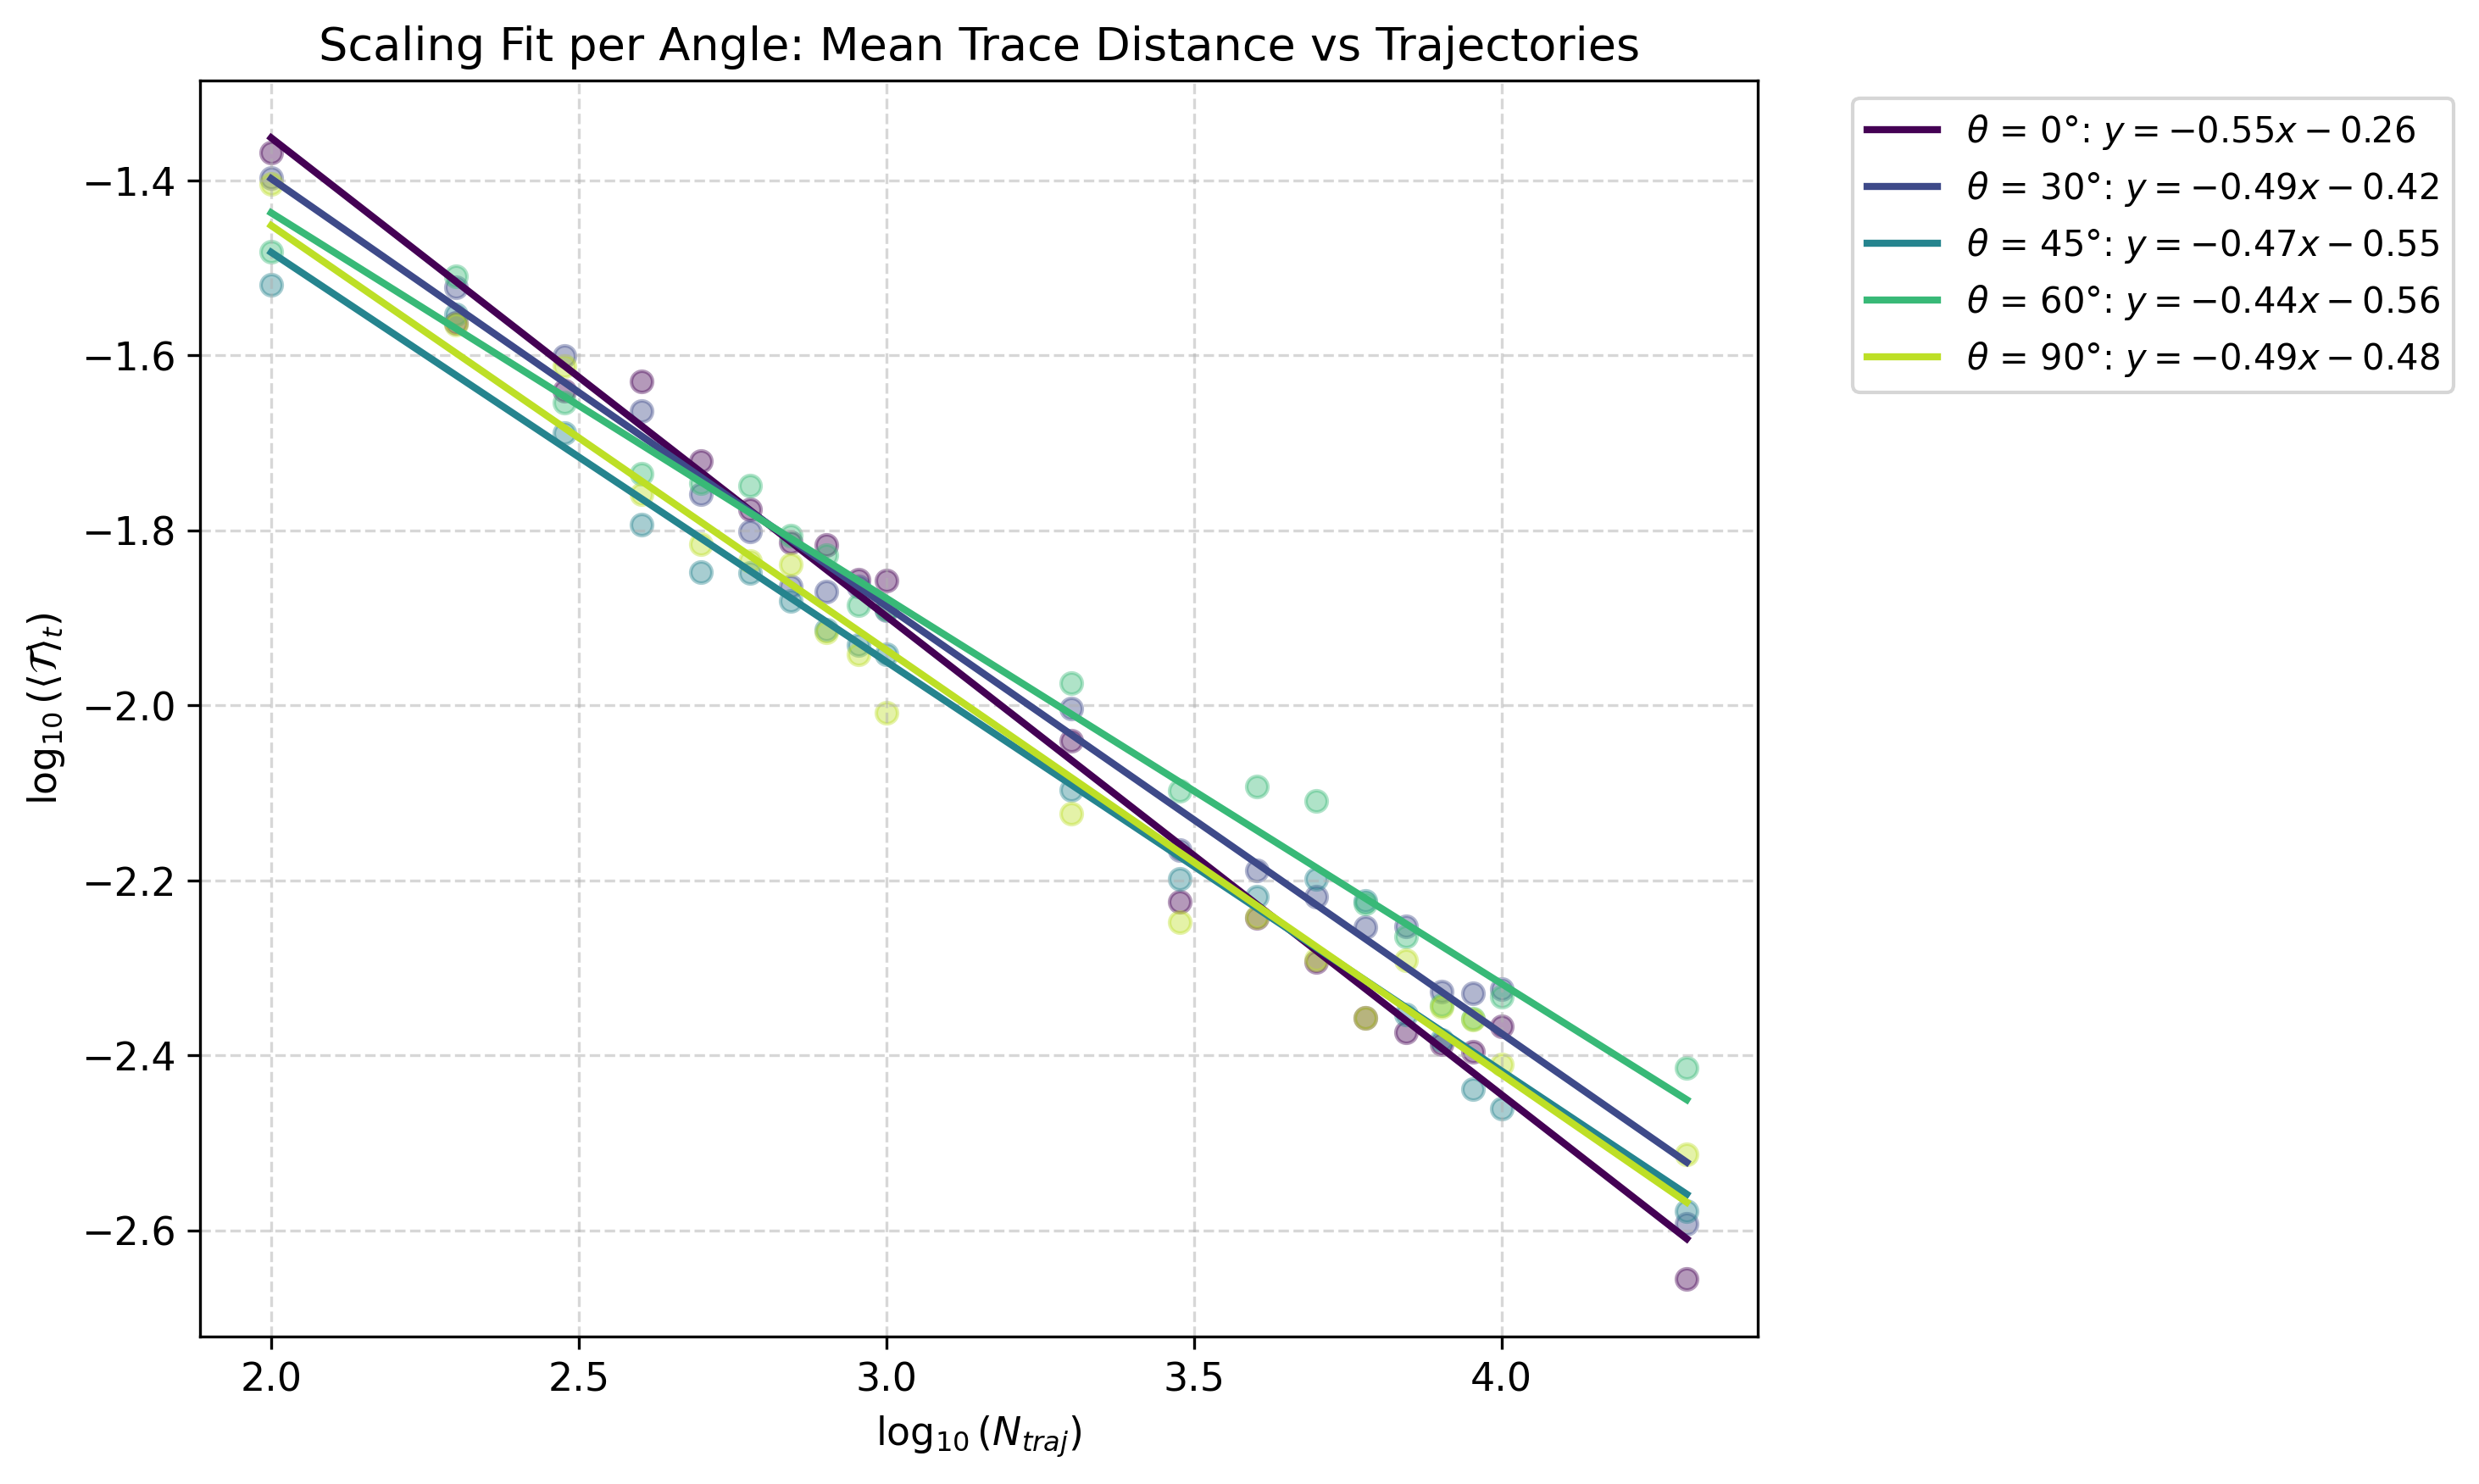
\includegraphics[width=\textwidth]{Angle_Fits_Mean_Trace_Distance_normal.png}
	\label{fig:Fitting_Trace_Distance_Avg_in_time}
	\caption{Linear Fitting of the values of $ \langle \mathcal{T} \left( \rho^{L}, \sigma^{A} \right) \rangle_{t} $ for different values of $ N_{Traj} $ and $ \theta $}
\end{figure} BARRE ERRORE
Considering the error bar is possible to assume that there's no substantial difference between different unraveling scheme, so that we can use all the values together for the fitting, in order to have more point and obtaining a more correct result : 
\begin{figure}[H]
	\centering
	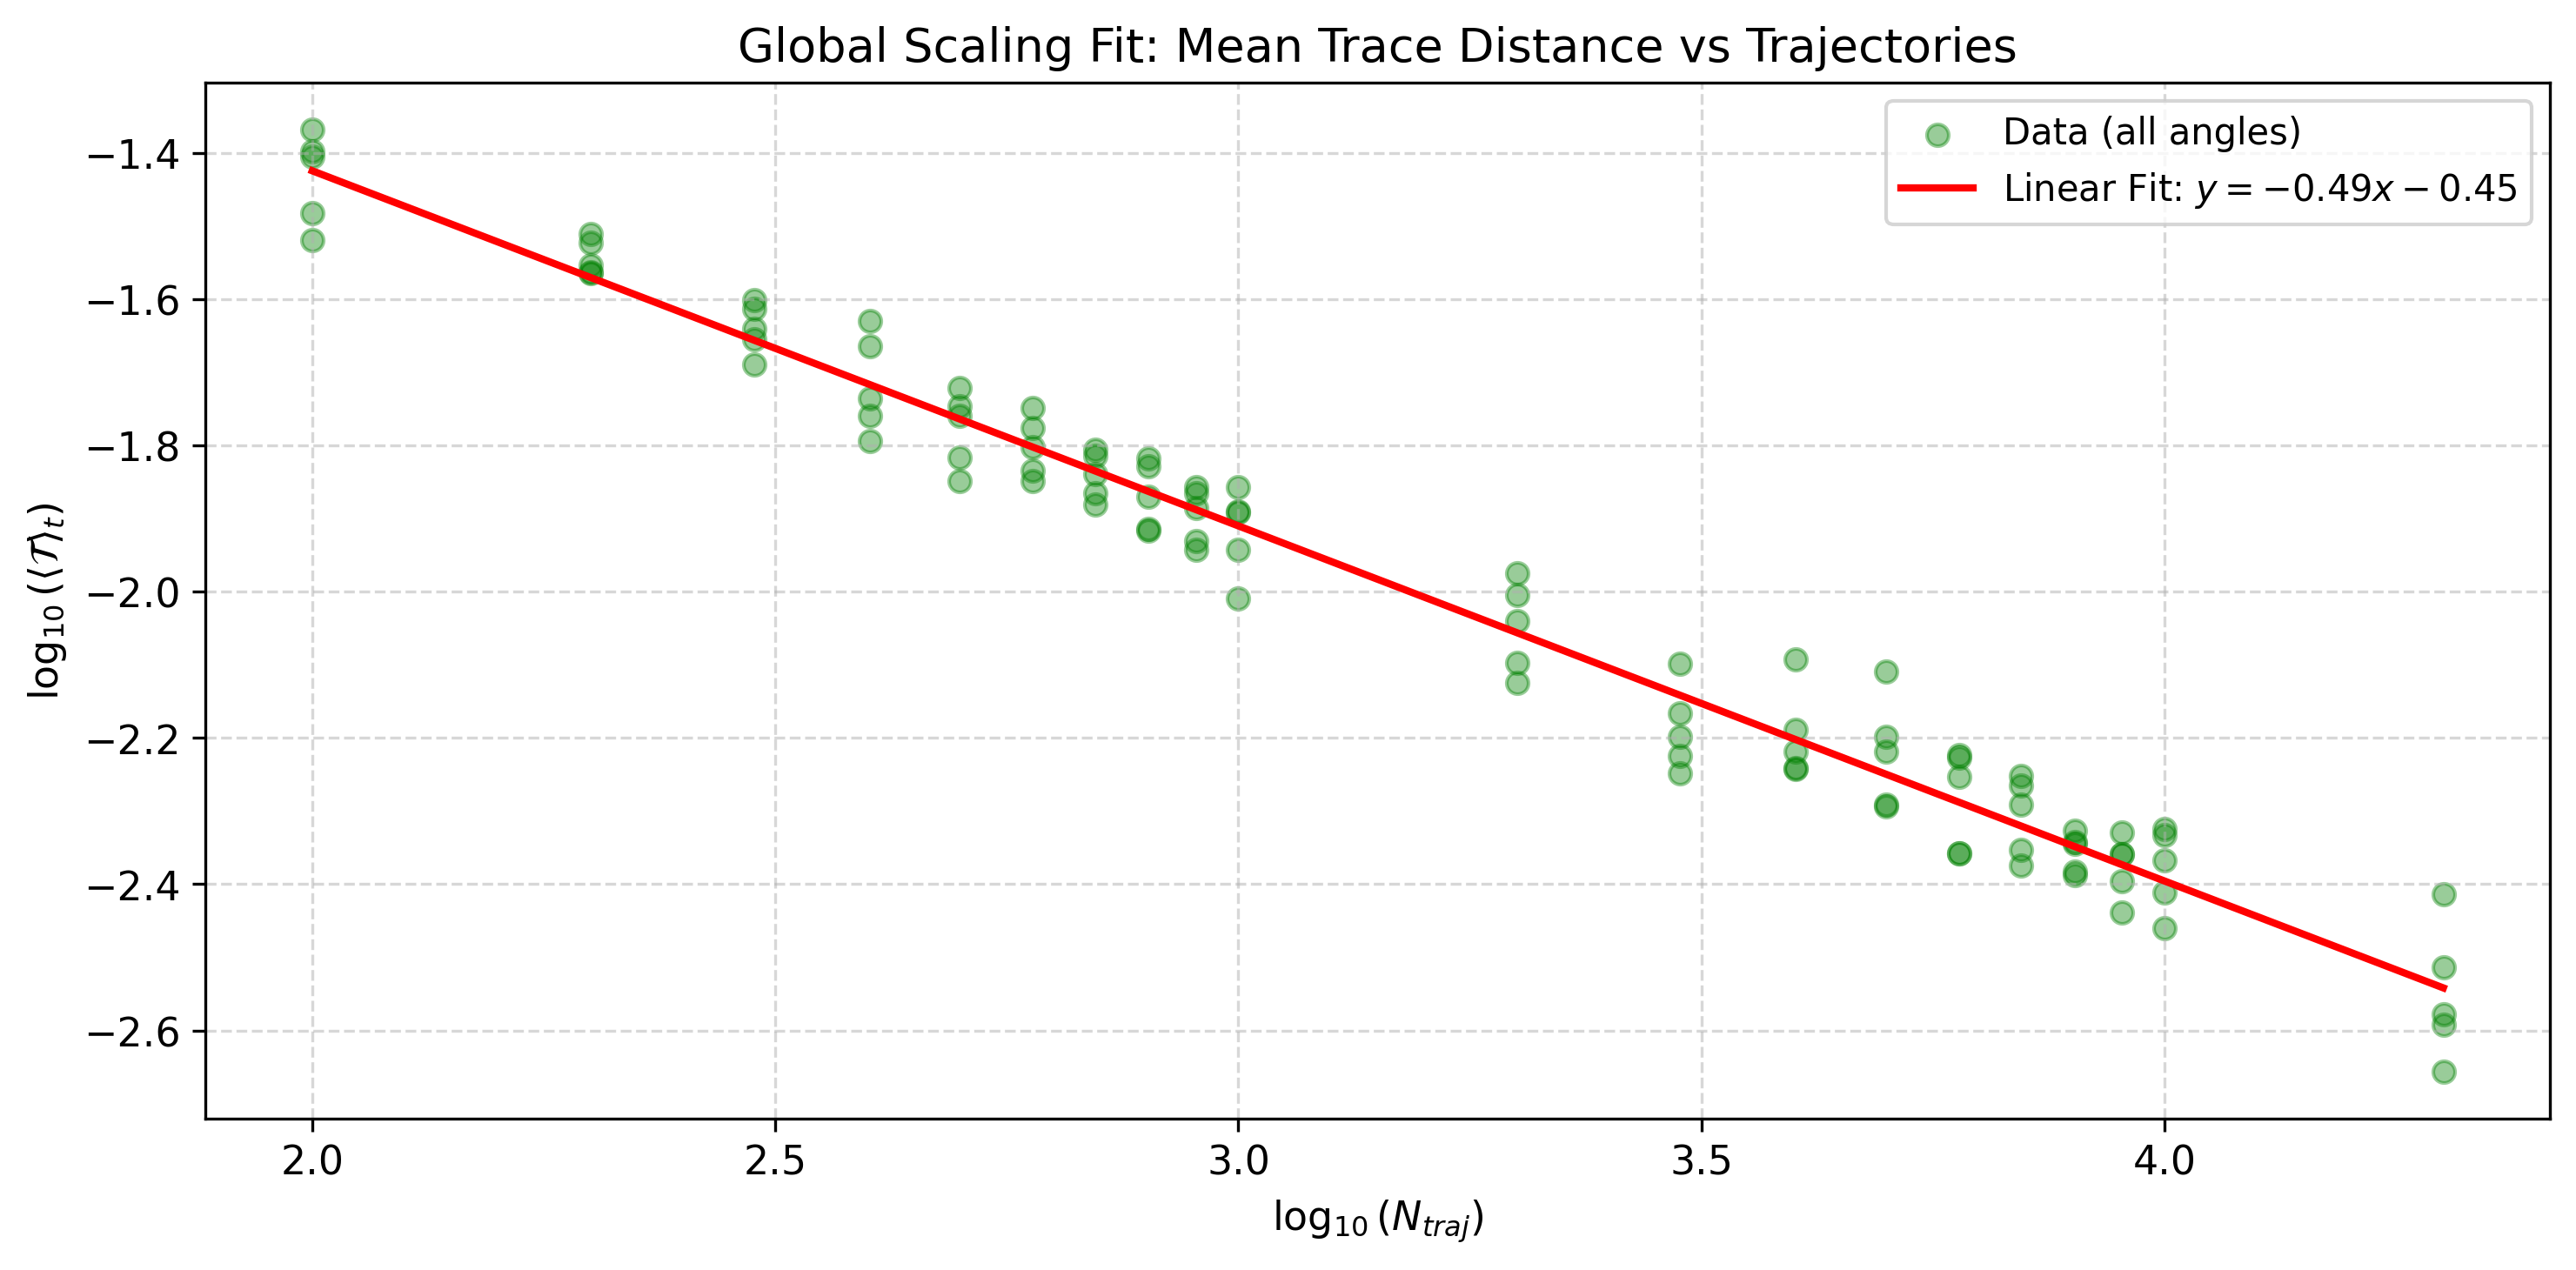
\includegraphics[width=\textwidth]{Global_Fit_Mean_Trace_Distance_normal.png}
	\label{fig:Global_Fitting_Trace_Distance_Avg_in_time}
	\caption{Linear Fitting of the values of $ \langle \mathcal{T} \left( \rho^{L}, \sigma^{A} \right) \rangle_{t} $ for different values of $ N_{Traj} $ and $ \theta $}
\end{figure}
The equation associated to the Linear Fitting is :
\begin{align}
		\log{\left(\langle \mathcal{T}\rangle_{t}\right)} &= q + m \log{\left(N_{Traj}\right)} \\
	\mathcal{T} &= e^{q} \left(N_{Traj}\right)^{m} \\
	&= e^{-0.45} \left(N_{Traj}\right)^{-0.5}
\end{align} 
The trace distance serves as a rigorous metric to quantify the statistical error $\varepsilon$ between the empirical average of the simulated trajectories and the exact deterministic state governed by the Lindblad master equation. Because these stochastic trajectories are generated via a Monte Carlo algorithm, they constitute a set of independent and identically distributed (i.i.d.) random variables. Consequently, the convergence of their sample mean is governed by the \textbf{\textit{Central Limit Theorem}} (CLT), which states that:
\begin{quote}
	For a sufficiently large number of independent samples $N$, the distribution of the sample mean approaches a normal distribution, regardless of the underlying probability distribution of the individual samples. In the context of Monte Carlo simulations, this implies that the statistical error $\varepsilon$ between the estimated average and the true expected value scales asymptotically inversely with the square root of the number of trajectories:
	$$ \varepsilon = \frac{\sigma_{Std}}{\sqrt{N}} $$
\end{quote}
The \textit{slope m} value of the Linear Regression confirms the dependence of $ \left(\langle \mathcal{T}\rangle_{t}\right) $ on $\sqrt{N}$, confirming the purely statistical nature of the numerical error. Moreover the value of the \textit{intercept q} is related to the \textit{Standard Deviation} like :
\begin{equation}
	e^{q} = \sigma_{Std} = \sqrt{\frac{\sum_{n}^{N}\left(\chi_{n} - \mu\right)^{2}}{N}}
\end{equation}
where $ \chi_{n} = \sigma^{n} = \ket{\psi_{S}^{n}}\bra{\psi_{S}^{n}} $
associated to the single n-th trajectory, while $ \mu = \rho^{L} $. \newline
Evaluating the \textit{Standard Deviation} or the \textit{Variance}, (define as $ \text{Var}(x) = \sigma_{Std}^{2}(x) = \mathbb{E}[x^2] - (\mathbb{E}[x])^2 $ ) of an observable can give us direct information on the error associated with the mean for that specific observable; if unraveling schemes lead to different variances, it is possible to choose the most favorable scheme for that observable, i.e. the one that, having the smallest variance, also has the smallest error, for the same number of sampled trajectories.

Crucially, because the trace distance provides a strict upper bound on the difference in expectation values for any bounded operator, the statistical error scaling guaranteed by the Central Limit Theorem for the density matrix directly translates to a robust upper bound on the error for any physical observable extracted from the system.

To practically demonstrate the advantage described above, the time evolution of the variance was analyzed for the Crucially, because the trace distance provides a strict upper bound on the difference in expectation values for any bounded operator, the statistical error scaling guaranteed by the Central Limit Theorem for the density matrix directly translates to a robust upper bound on the error for any physical observable extracted from the system., corresponding to the expectation values of the Pauli matrices $\langle \sigma_x \rangle$, $\langle \sigma_y \rangle$, $\langle \sigma_z \rangle$, for different unraveling scheme. By simulating an ensemble of $N = 20,000$ trajectories, it is possible to map the statistical fluctuations along the different quantization axes and directly compare the noise profiles intrinsic to the chosen collisional unraveling algorithm. 

\newpage

In the following figure we are plotting the Variance over time of $\langle \sigma_x \rangle$, $\langle \sigma_y \rangle$, $\langle \sigma_z \rangle$ for different value of $ \theta $ : 
\begin{figure}[H]
	\centering
	\begin{subfigure}[b]{0.48\textwidth}
		\centering
		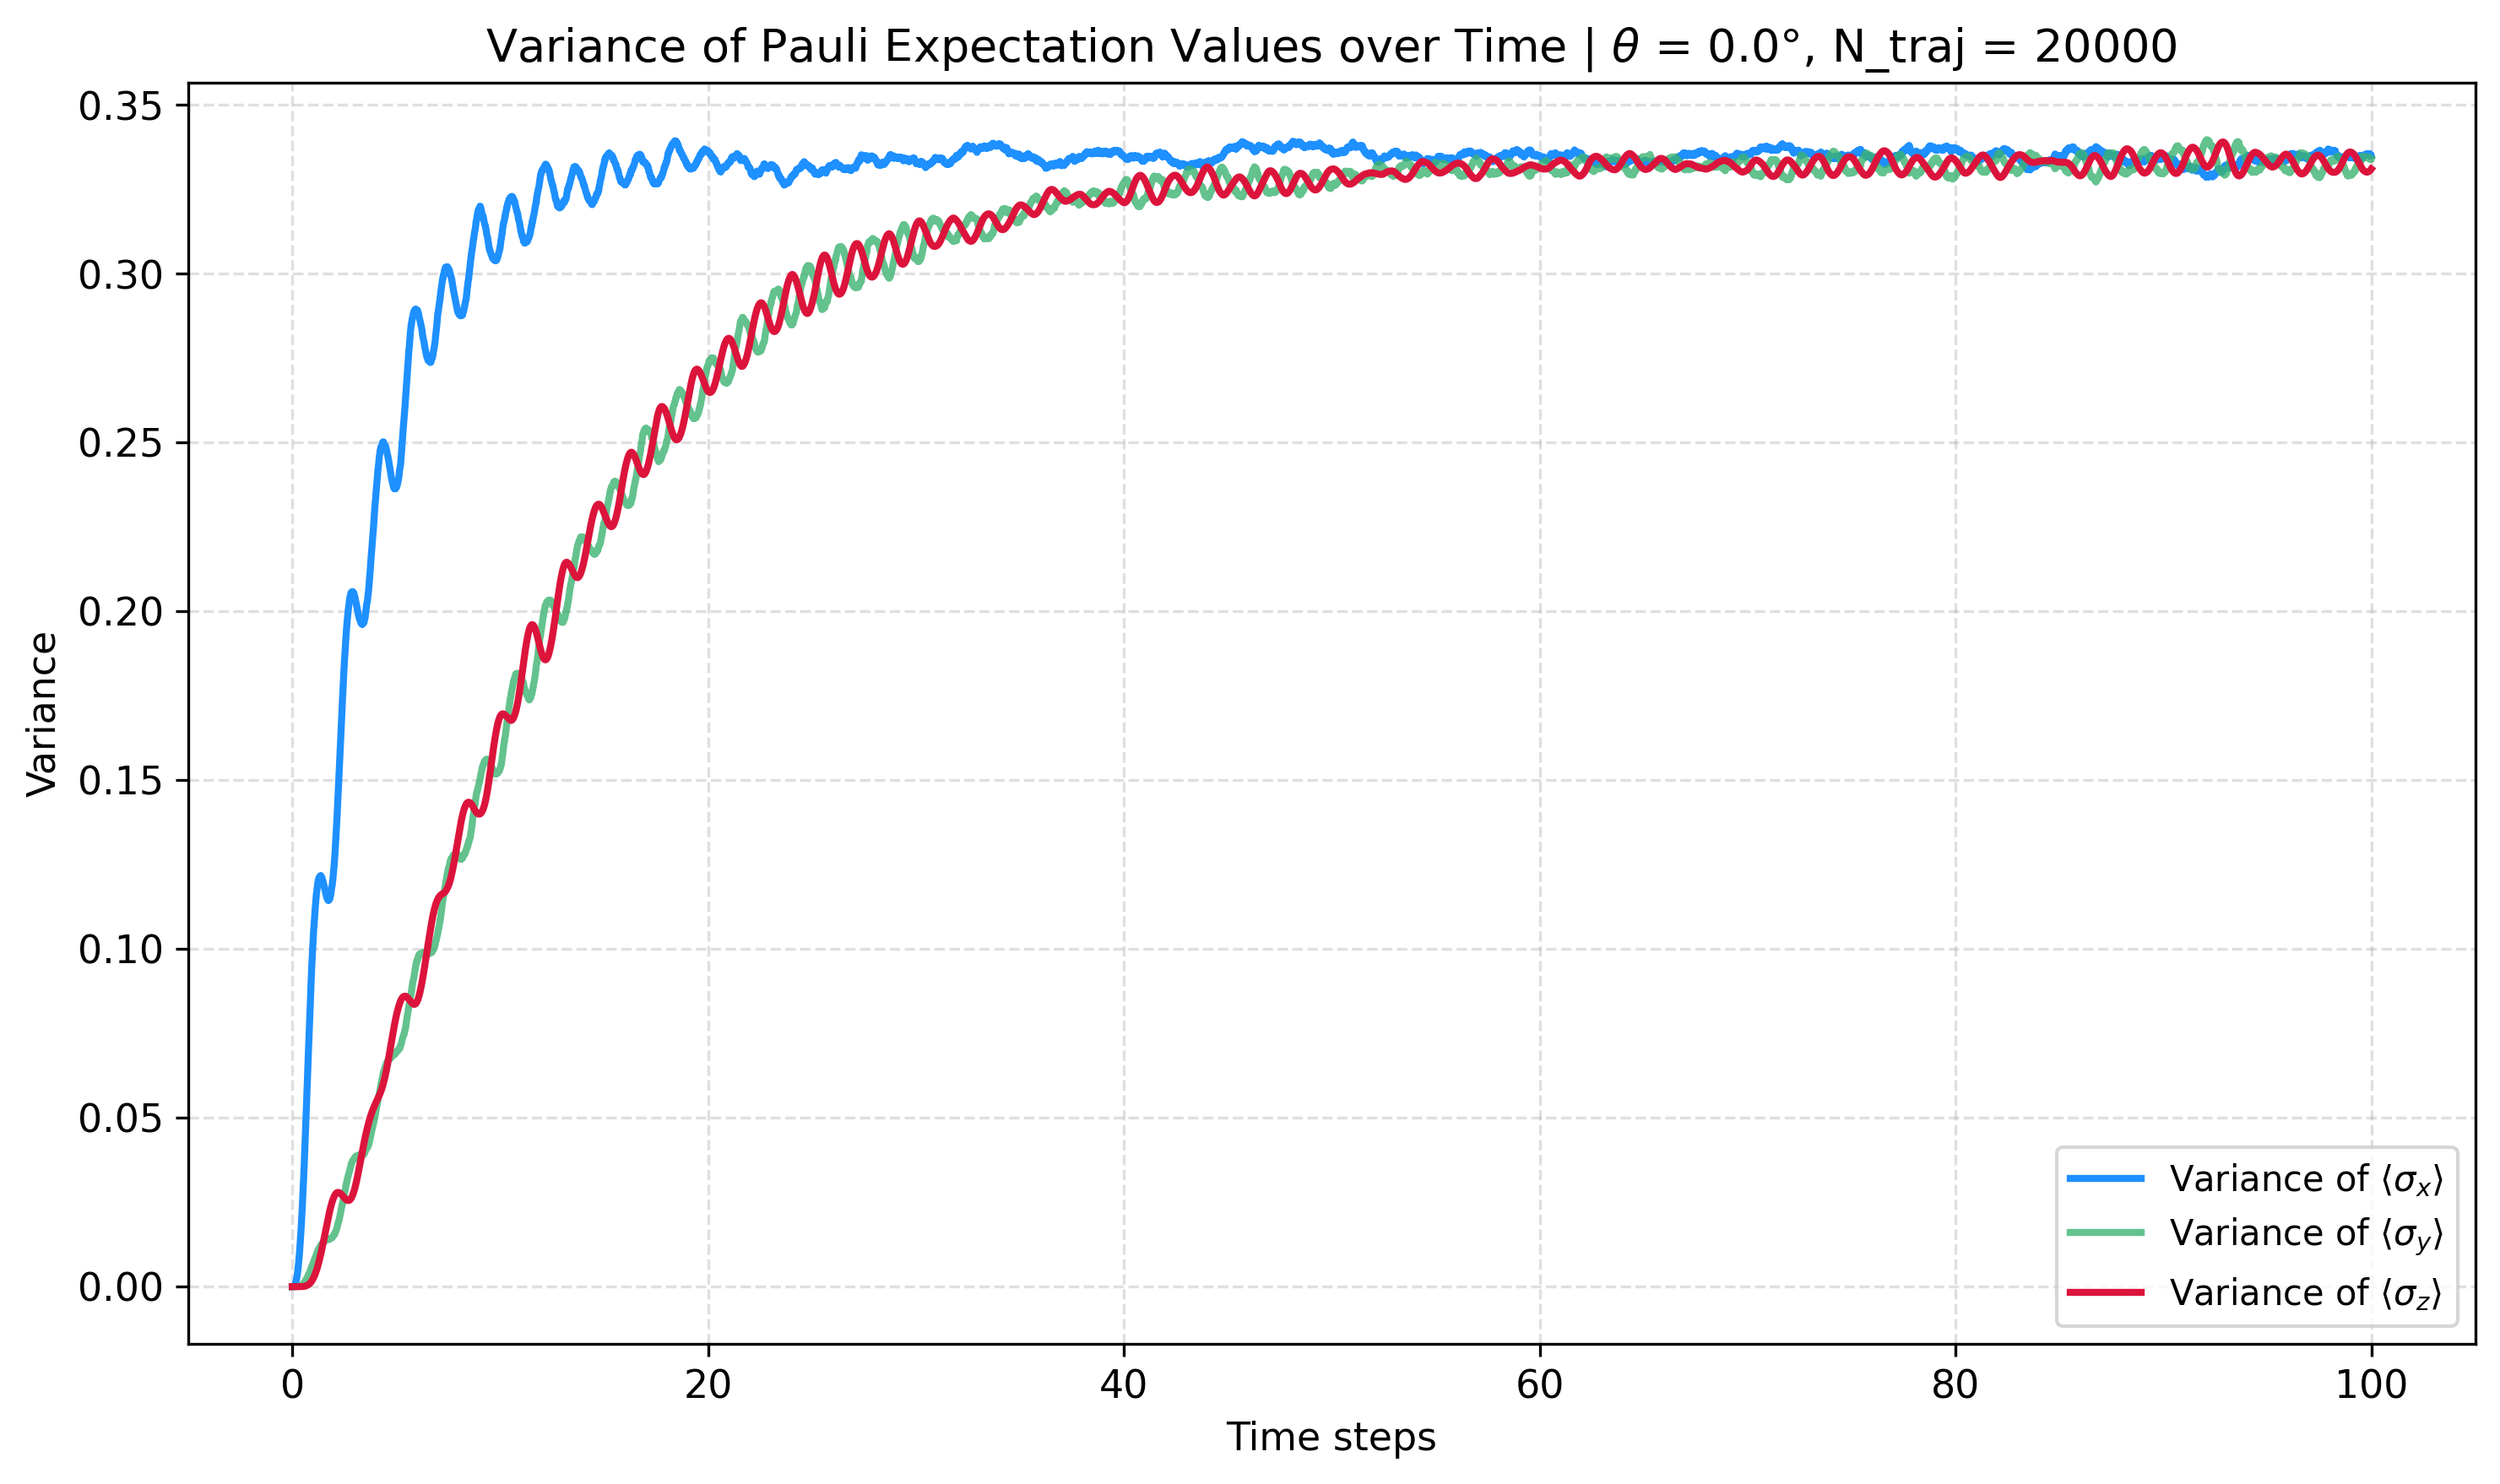
\includegraphics[width=\textwidth]{Variance_Pauli_Theta_0p000000_dt_0p010000_N_traj_20000.png}
		\label{fig:panel_a_Var_Sxyz_0_deg}
		\caption{}
	\end{subfigure}
	\hfill
	\begin{subfigure}[b]{0.48\textwidth}
		\centering
		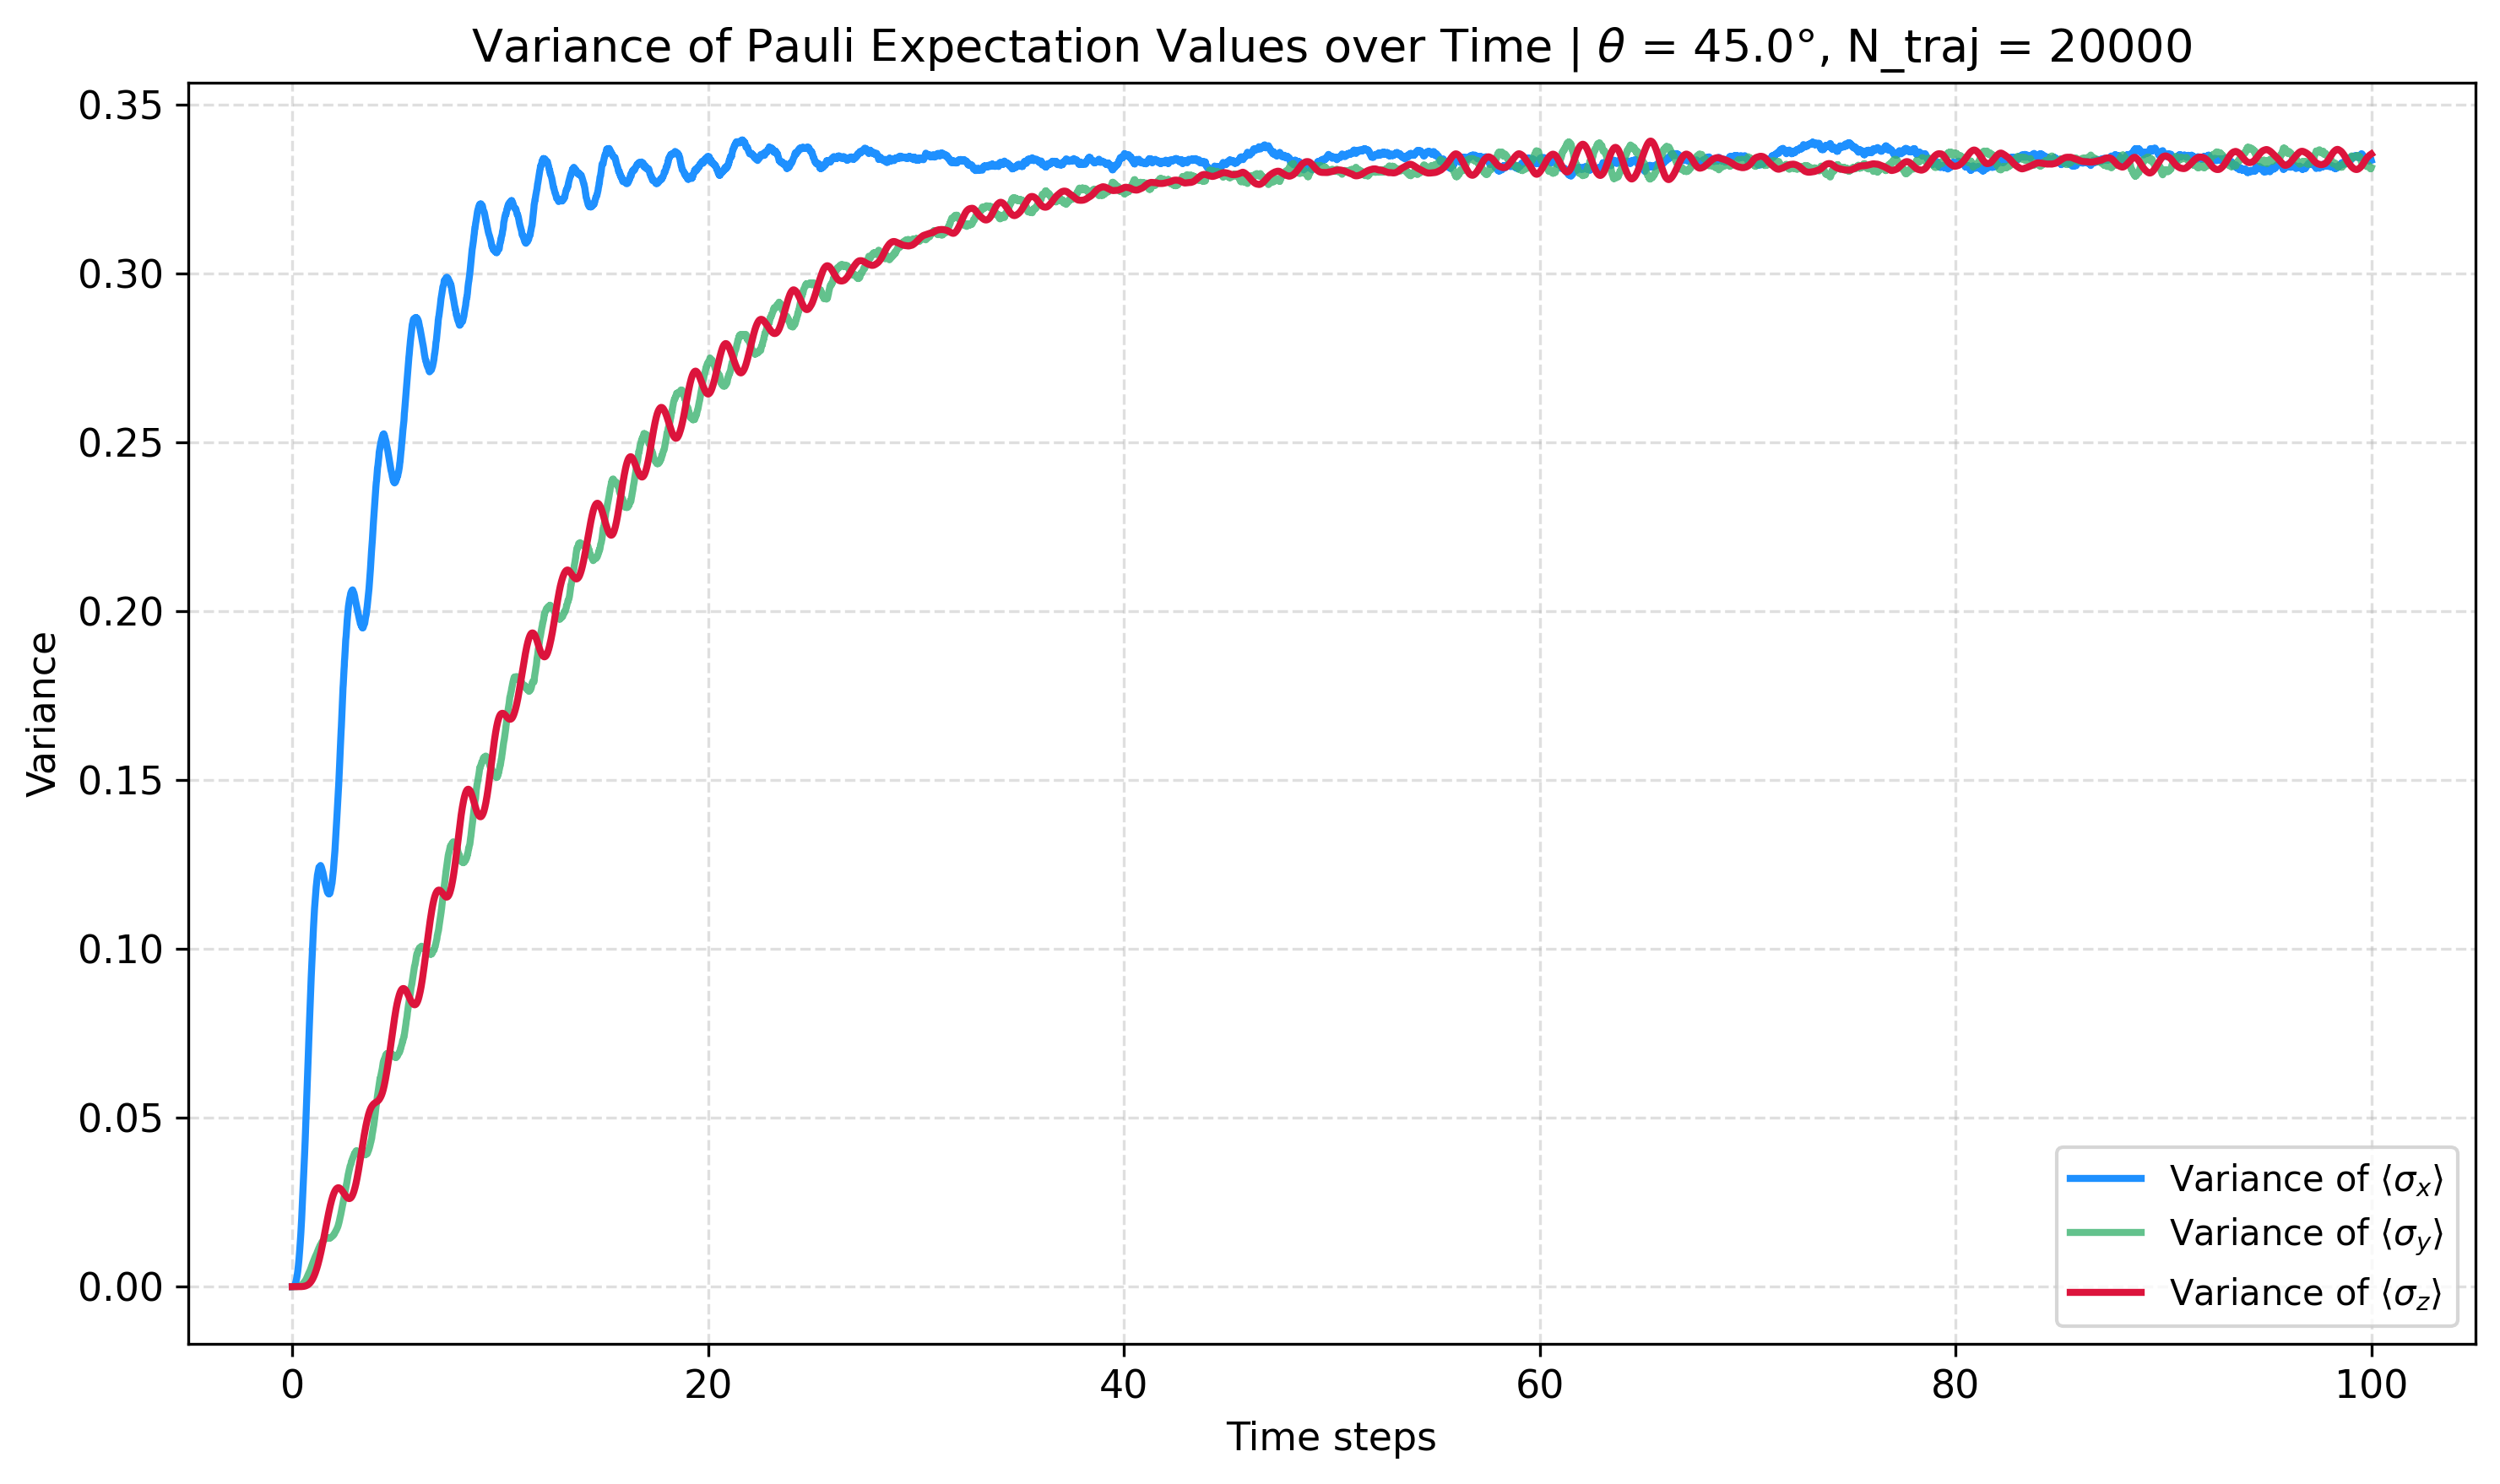
\includegraphics[width=\textwidth]{Variance_Pauli_Theta_0p785398_dt_0p010000_N_traj_20000.png}
		\label{fig:panel_b_Var_Sxyz_45_deg}
		\caption{}
	\end{subfigure}
	\hfill
	\begin{subfigure}[b]{0.48\textwidth}
		\centering
		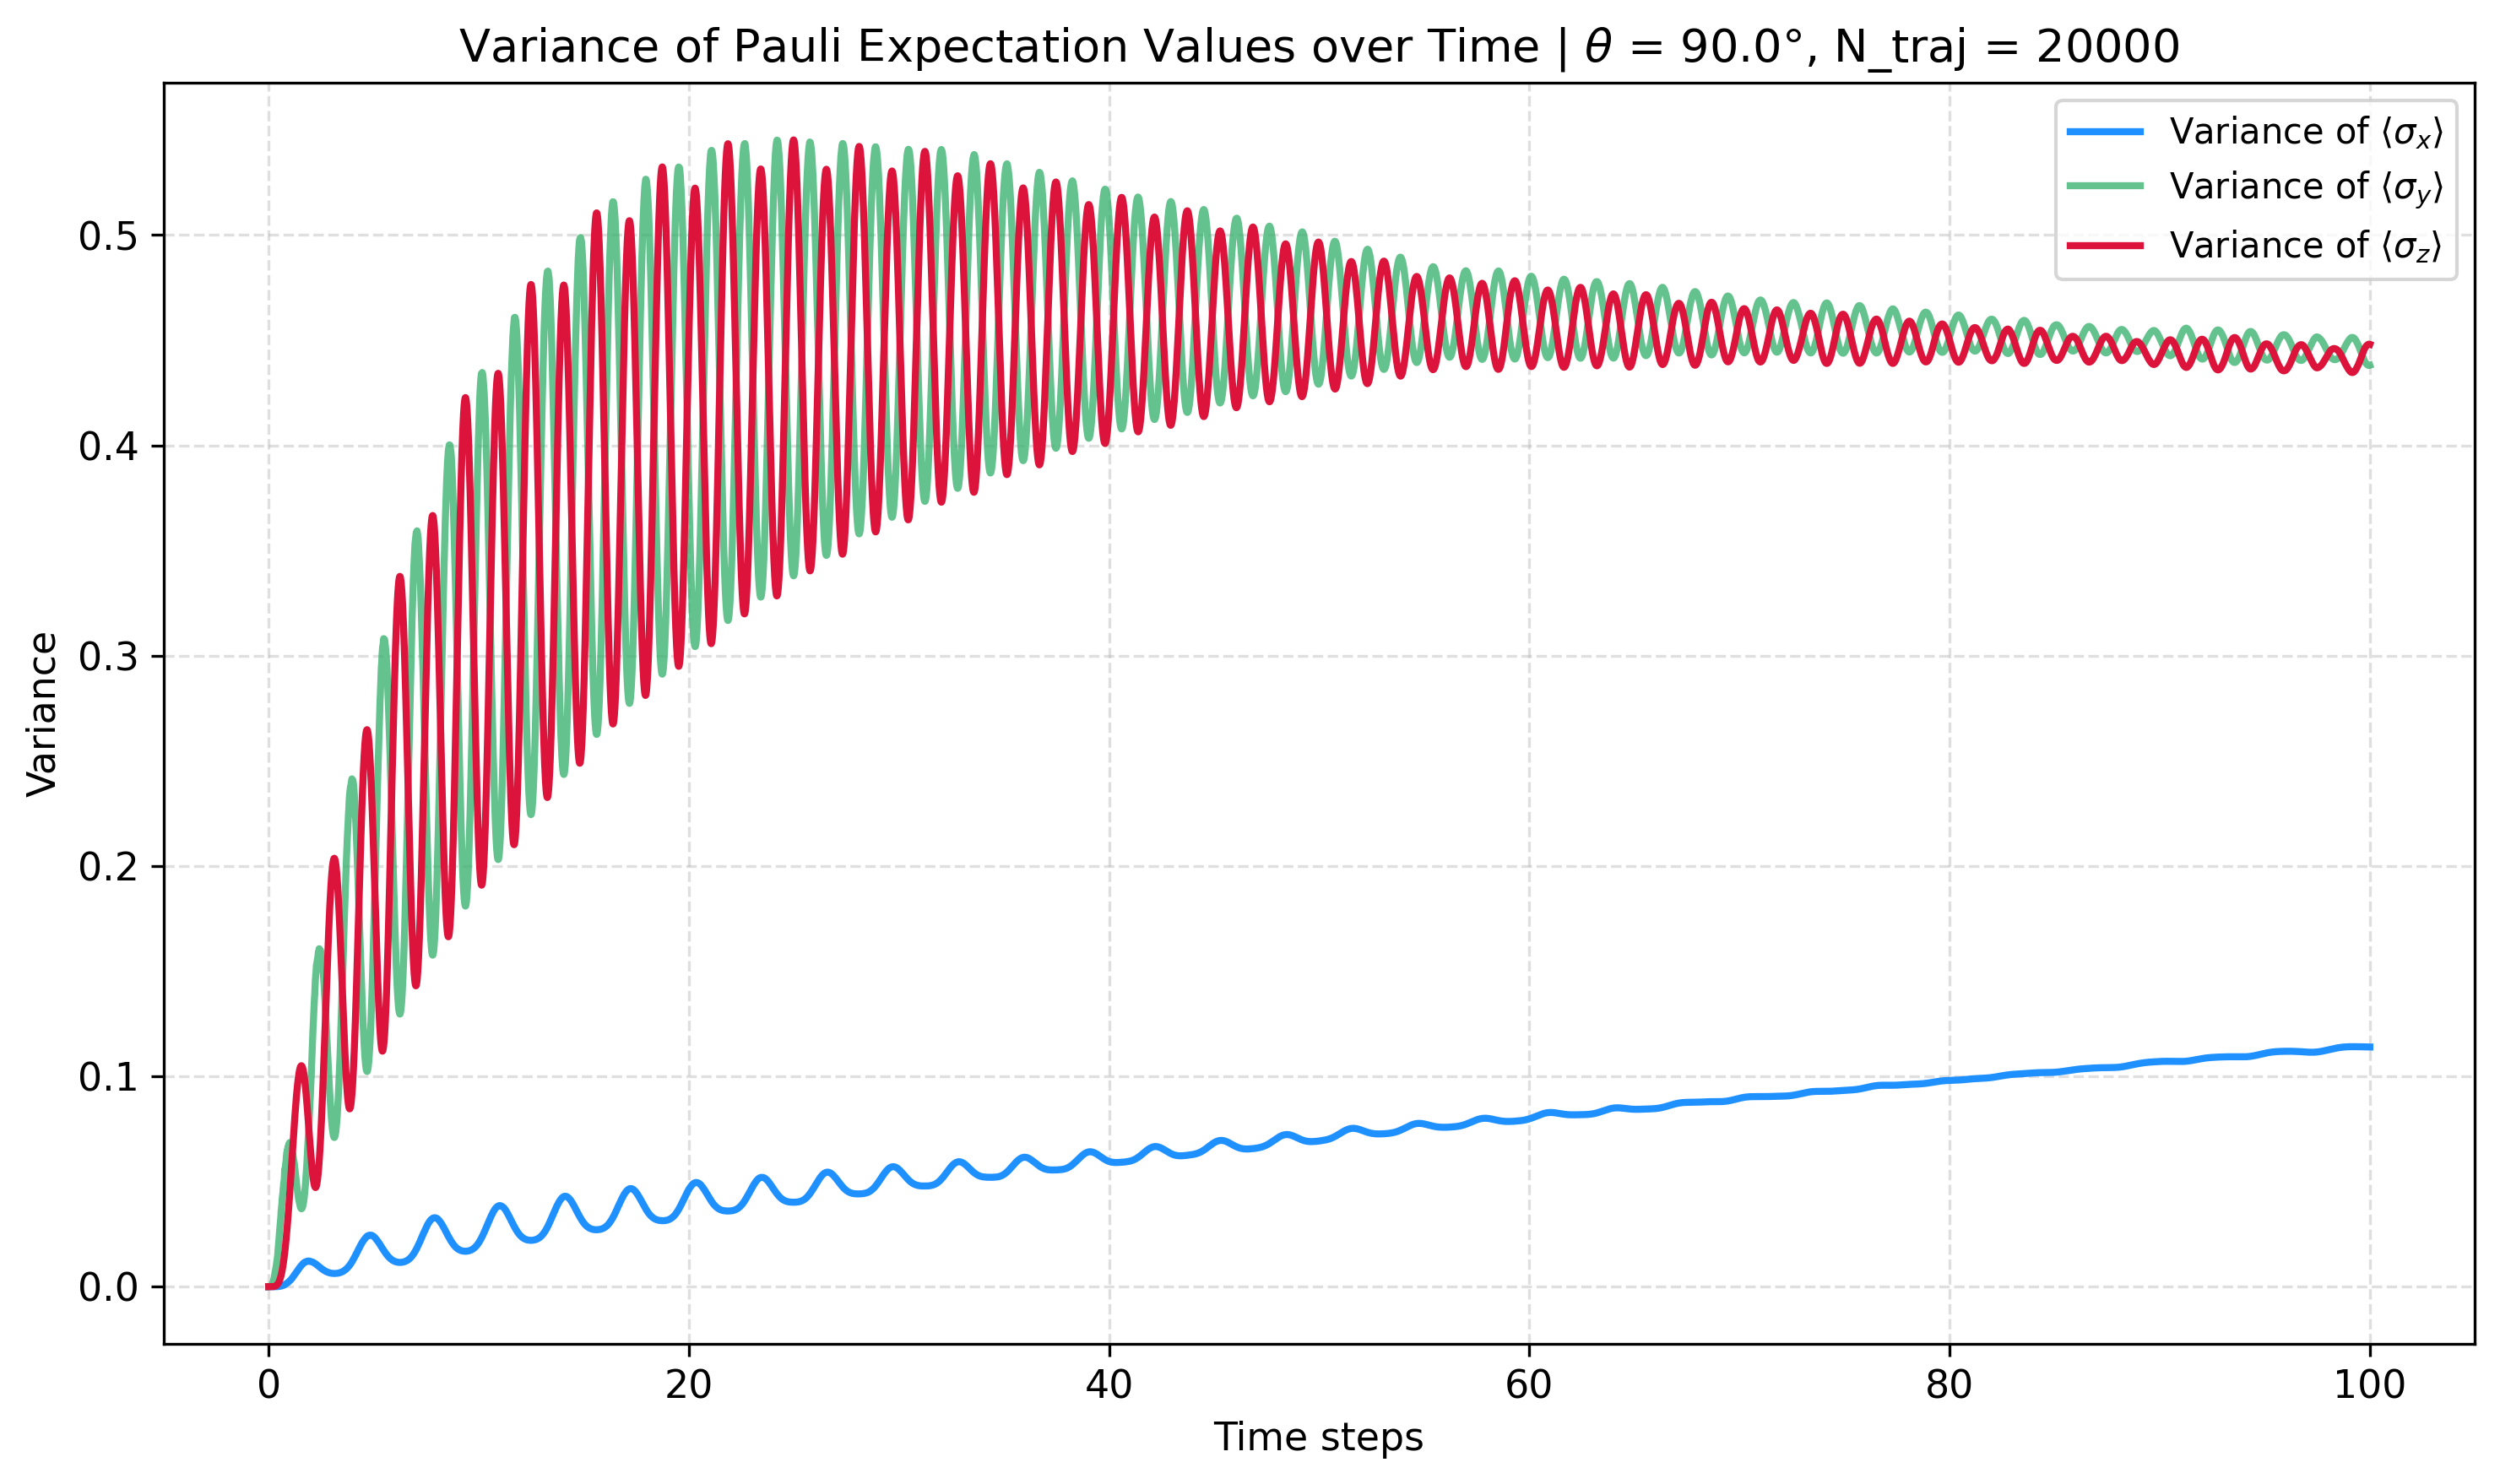
\includegraphics[width=\textwidth]{Variance_Pauli_Theta_1p570796_dt_0p010000_N_traj_20000.png}
		\label{fig:panel_c_Var_Sxyz_90_deg}
		\caption{}
	\end{subfigure}
	\caption{Variance over time for the three components of the Bloch vector, calculated for a) $ \theta = 0.0^{\circ} $ \textit{Sate Diffusion Limit}, b) $ \theta = 45.0^{\circ} $ general intermediate regime, c) $ \theta = 90.0^{\circ} $ \textit{Quantum Jump Limit}}
\end{figure}
For all angles $\theta < 86.0^{\circ}$, the variance profiles are largely consistent with those reported for $\theta = 0.0^{\circ}$, which corresponds to the \textit{State Diffusion} (SD) limit. In this regime, we observe a slightly larger variance for $\langle \sigma_x \rangle$ compared to $\langle \sigma_y \rangle$ and $\langle \sigma_z \rangle$. \newline
The observed oscillations are associated with the coherent dynamics of the system.

Moving towards the \textit{Quantum Jump} (QJ) limit ($\theta \to 90^{\circ}$), we observe a drastic change in both the absolute values and the oscillatory behavior of the variance. Specifically, the variance of $\langle \sigma_x \rangle$ is significantly suppressed and appears not to have reached convergence within the simulated time window. Conversely, $\langle \sigma_y \rangle$ and $\langle \sigma_z \rangle$ reach much higher variance peaks, characterized by prominent, high-frequency oscillations.

To justify this complex behavior, we must focus on the interplay between the system's coherent dynamics and the effective form of the \textit{Kraus operators} $\mathcal{M}_{0}^{j}$ and $\mathcal{M}_{1}^{j}$ (Eq.~\ref{eq:M0_simplified} and Eq.~\ref{eq:M1_simplified}). The coherent evolution in the single-exciton subspace, governed by the Hamiltonian $\mathcal{H}_{Exc}$, corresponds to a $\sigma_x$ operator. Geometrically, this induces a continuous rotation around the x-axis on the Bloch sphere; consequently, the isolated system trajectory is confined to the yz-plane, leaving the x-coordinate unvaried.

In the SD limit, the evolution dictated by $\mathcal{M}_{0}^{j}$ and $\mathcal{M}_{1}^{j}$ acts as a continuous, infinitesimal rotation around the z-axis. The direction of this rotation depends on the ancilla measurement outcome. Because these continuous stochastic rotations constantly push the state out of the yz-plane, non-zero x-components are continuously generated and dispersed. This results in a larger variance for $\langle \sigma_x \rangle$, which shares a similar temporal envelope with $\langle \sigma_y \rangle$ and $\langle \sigma_z \rangle$.

In the QJ limit, the dynamics is dominated by the deterministic isolated evolution, interrupted only by rare jump events when the ancilla is measured in the $\ket{1_a}$ state. A quantum jump applies a sudden, macroscopic rotation around the z-axis. When this jump occurs, it drastically alters the y-coordinate. However, since the system mostly evolves in the yz-plane (where the x-component is minimal), a sudden jump around the z-axis leaves the state inherently tied to the isolated dynamics plane, imparting only a minor perturbation along the x-axis. This suppression of out-of-plane stochastic diffusion perfectly justifies the remarkably low variance observed for $\langle \sigma_x \rangle$. The Excitonic Hamiltonian, which drives the rotation around the x-axis, immediately begins rotating this noisy y-component into the z-axis. This coherent coupling transfers the statistical fluctuations back and forth between the two axes, justifying the remarkably similar but phase-shifted variance profiles of $\langle \sigma_y \rangle$ and $\langle \sigma_z \rangle$.

Finally, the more intense oscillations of $\langle \sigma_y \rangle$ and $\langle \sigma_z \rangle$ can be attributed to the fact that, in the QJ regime, the terms $+i g_1 \sin(c_j \Delta t)\sigma_z^j$ and $-i g_0 \sin(c_j \Delta t)\sigma_z^j$ become dominant, since the ae the only ones present. These terms act as strong discrete phase-kicks that amplify the oscillatory noise of the system.

Furthermore, in the Quantum Jump limit ($\theta = 90^\circ$), it is evident that the variance of $\langle \sigma_x \rangle$ does not reach a steady-state plateau within the simulated time window. This behavior indicates that the relaxation time for the stochastic dynamics along the x-axis is orders of magnitude longer than for the y and z axes. Because the discrete jump operators primarily perturb the yz-plane, the x-axis remains largely decoupled from the environmental back-action. Consequently, the diffusion of statistical noise along this out-of-plane direction is extremely slow, implying that significantly longer simulation times would be required for this variance to eventually reach its asymptotic plateau.

A more specific analysis was also done for angles close to $ 90^{\circ} $, to see the behavior that is obtained by approaching the Quantum Jump Limit (of which we recall the uniqueness) : 
\begin{figure}[H]
	\centering
		\begin{subfigure}[b]{0.48\textwidth}
		\centering
		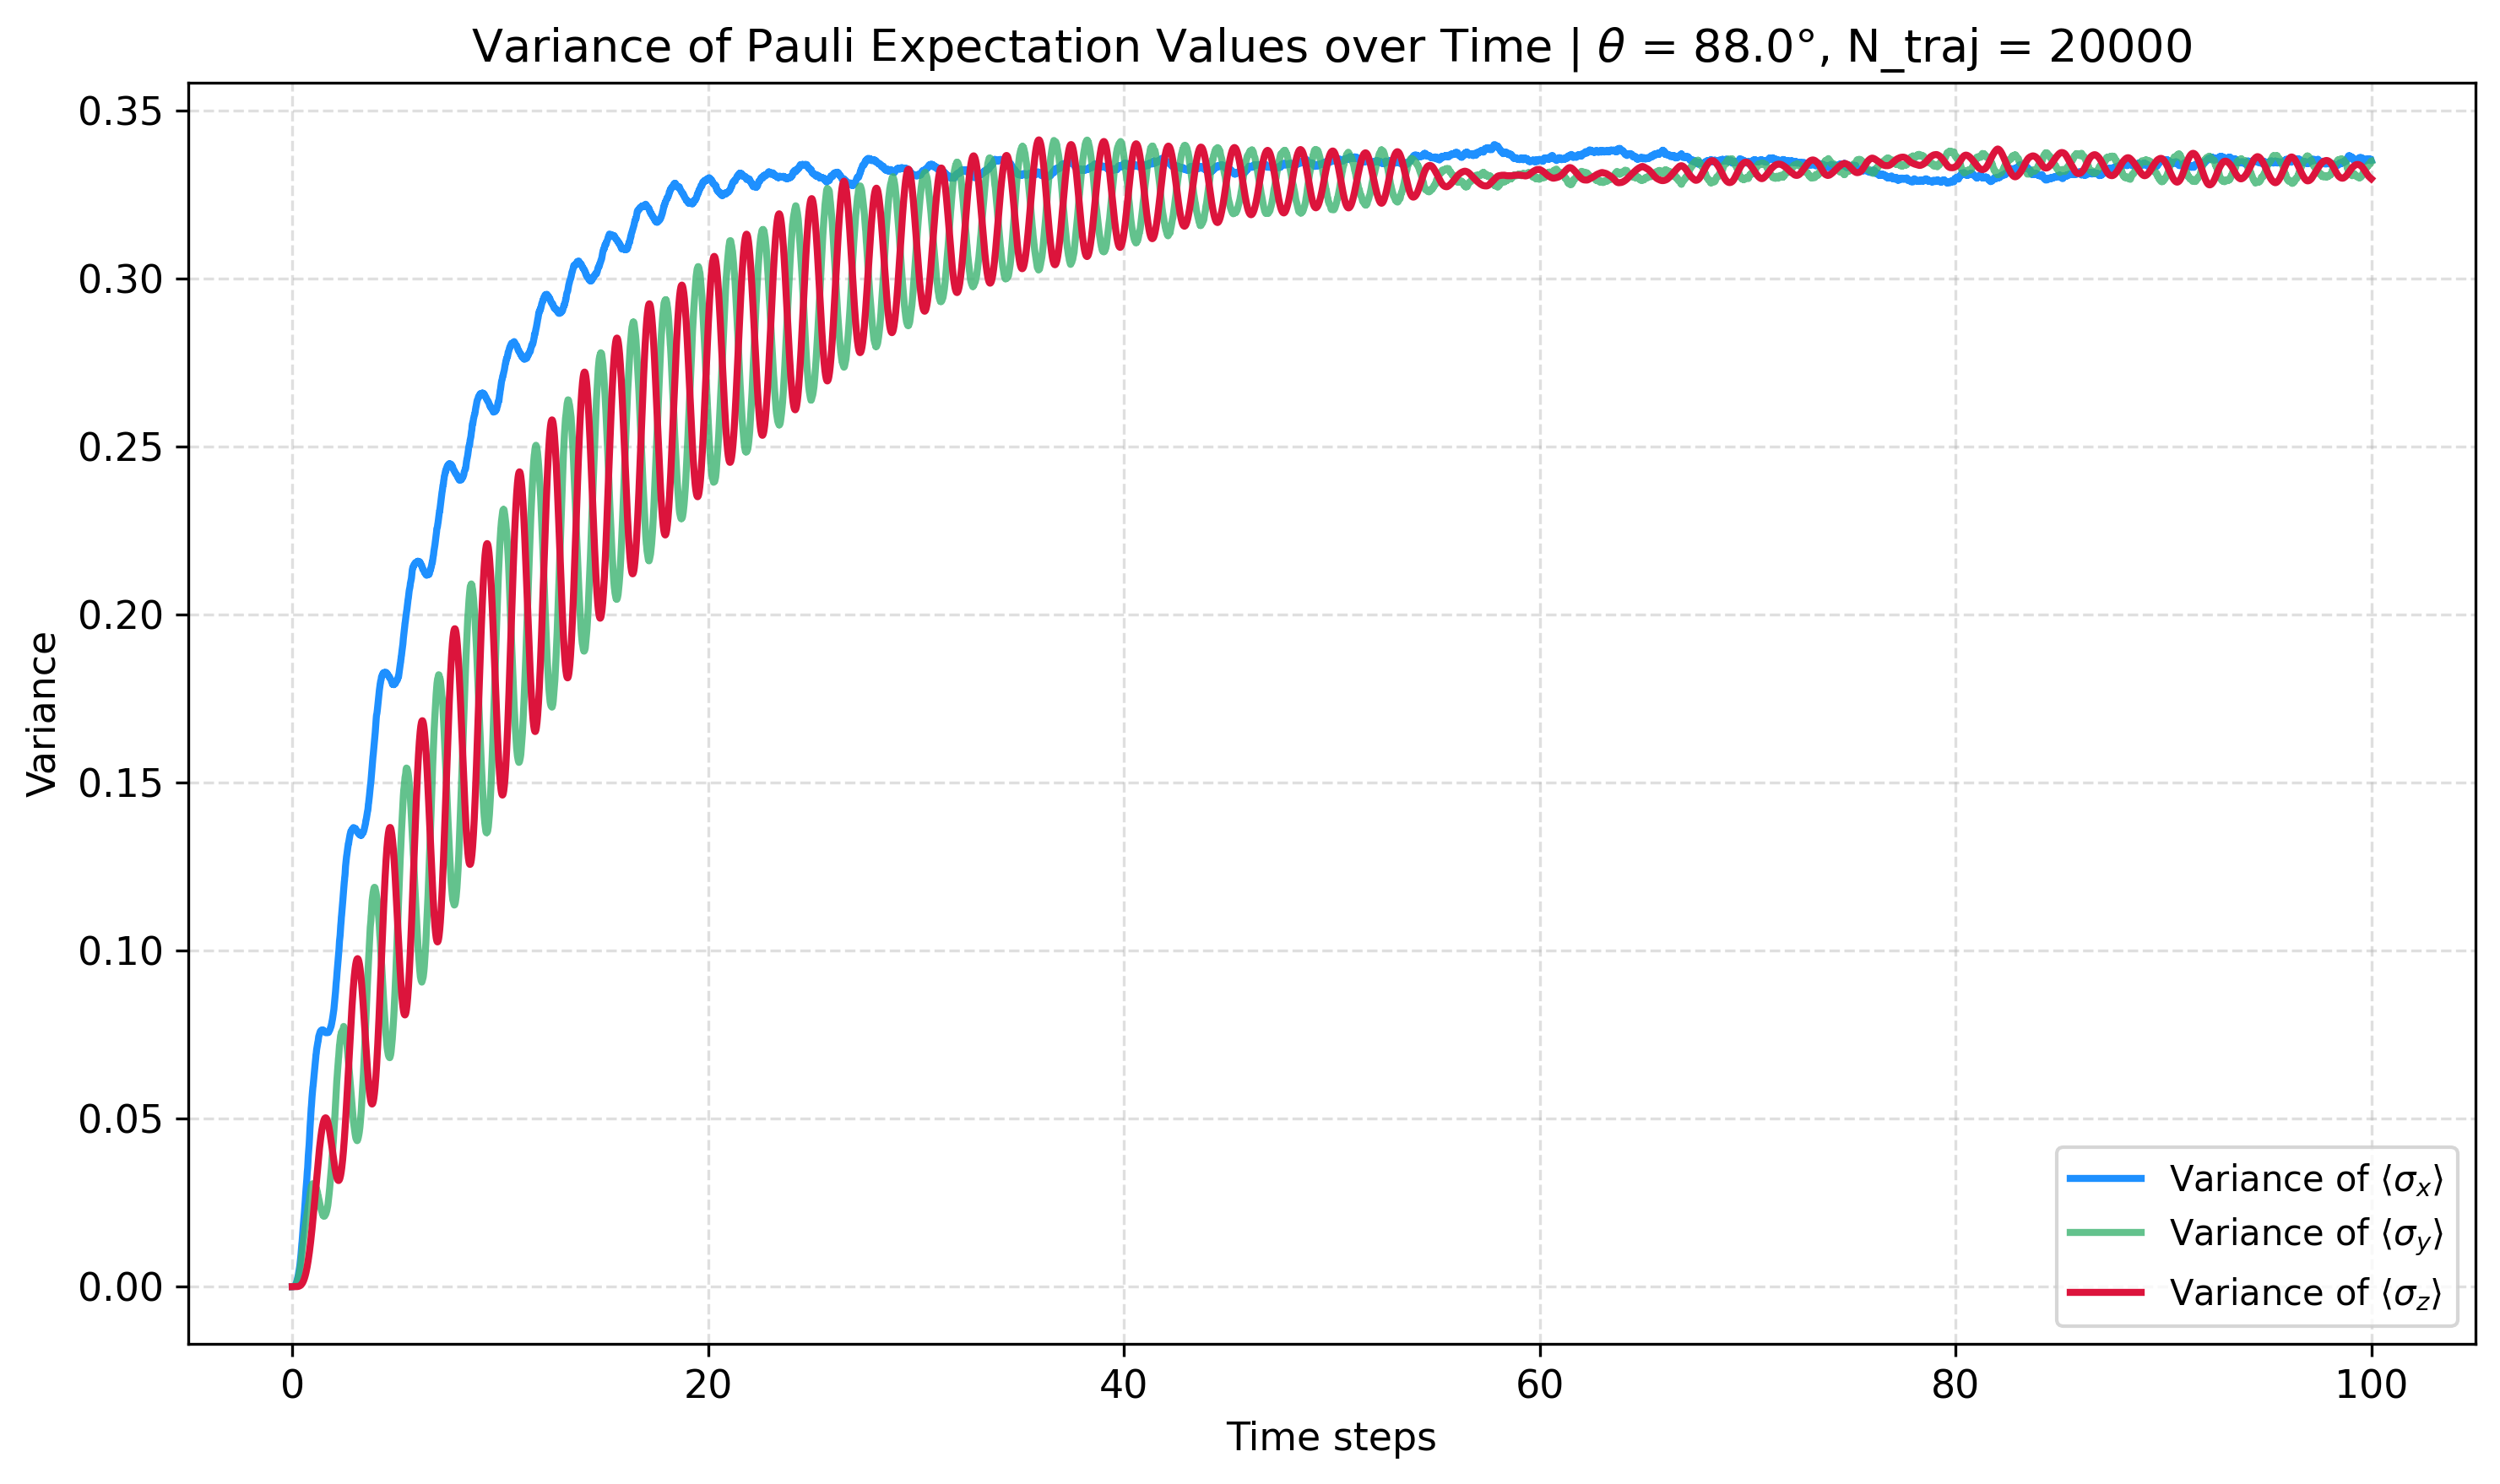
\includegraphics[width=\textwidth]{Variance_Pauli_Theta_1p535890_dt_0p010000_N_traj_20000.png}
		\label{fig:panel_a_Var_Sxyz_88_deg}
		\caption{}
	\end{subfigure}
	\hfill
	\begin{subfigure}[b]{0.48\textwidth}
		\centering
		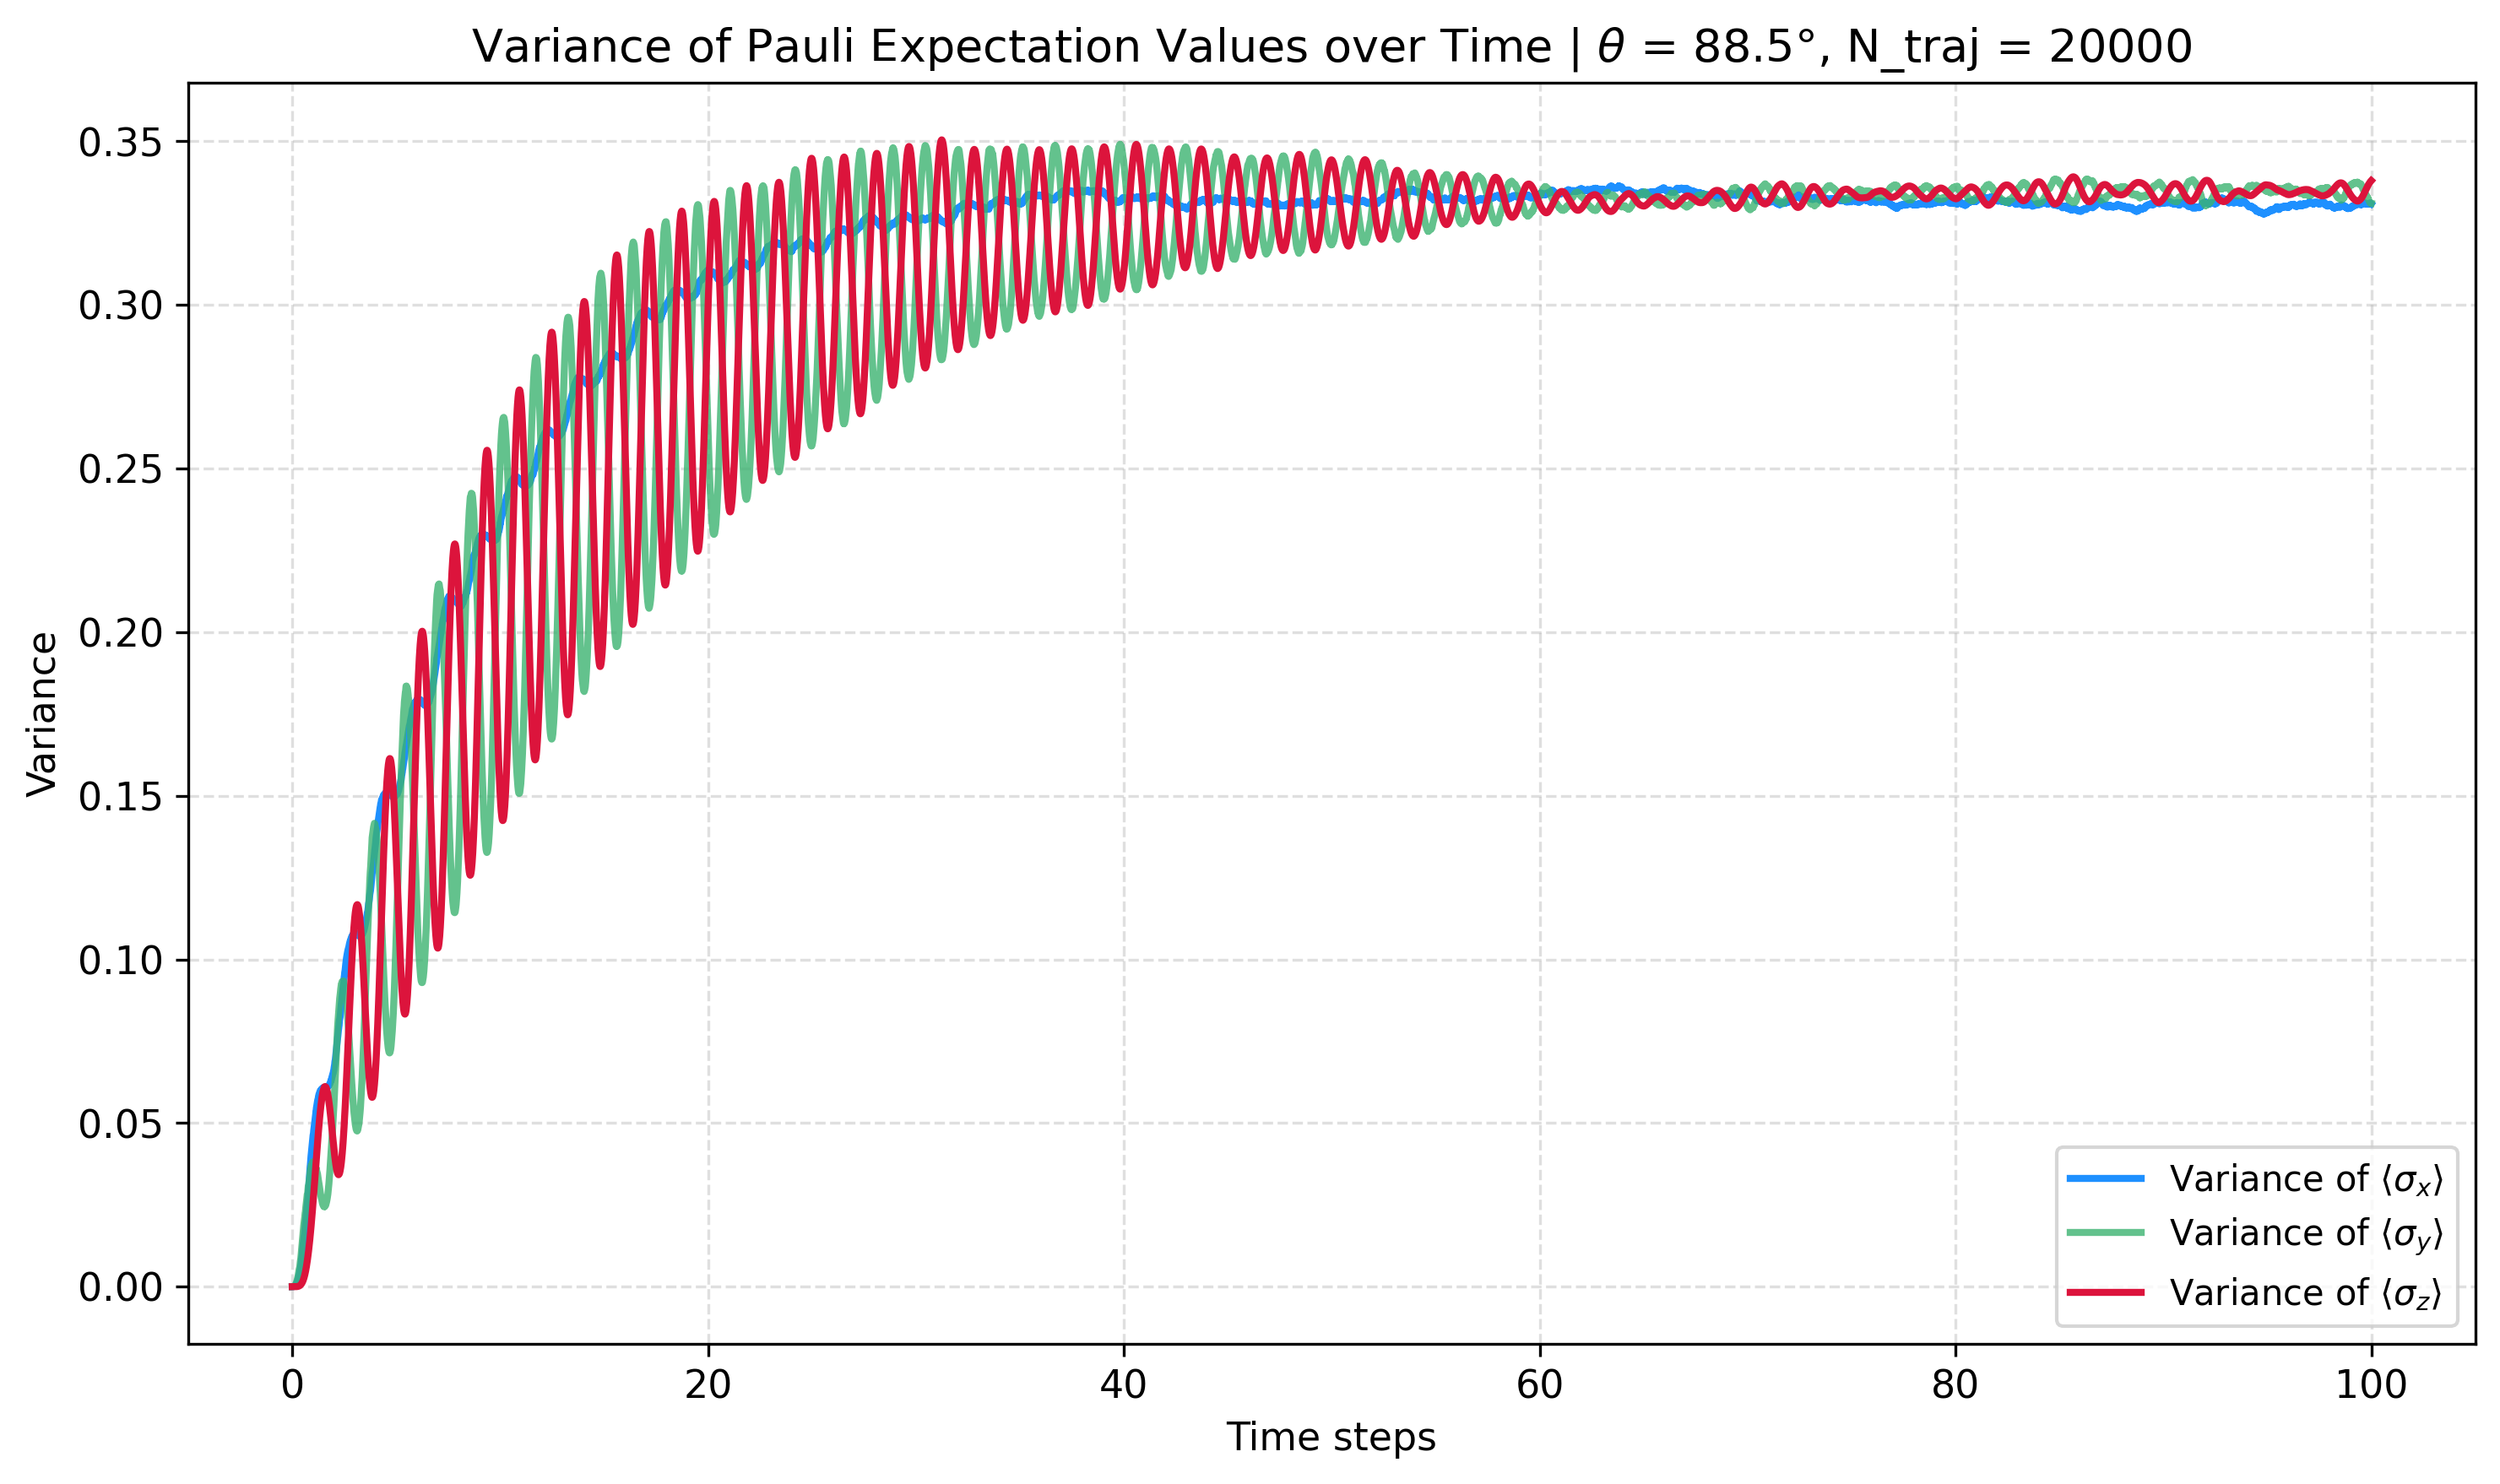
\includegraphics[width=\textwidth]{Variance_Pauli_Theta_1p544616_dt_0p010000_N_traj_20000.png}
		\label{fig:panel_b_Var_Sxyz_88.5_deg}
		\caption{}
	\end{subfigure}
	\hfill
	\begin{subfigure}[b]{0.48\textwidth}
		\centering
		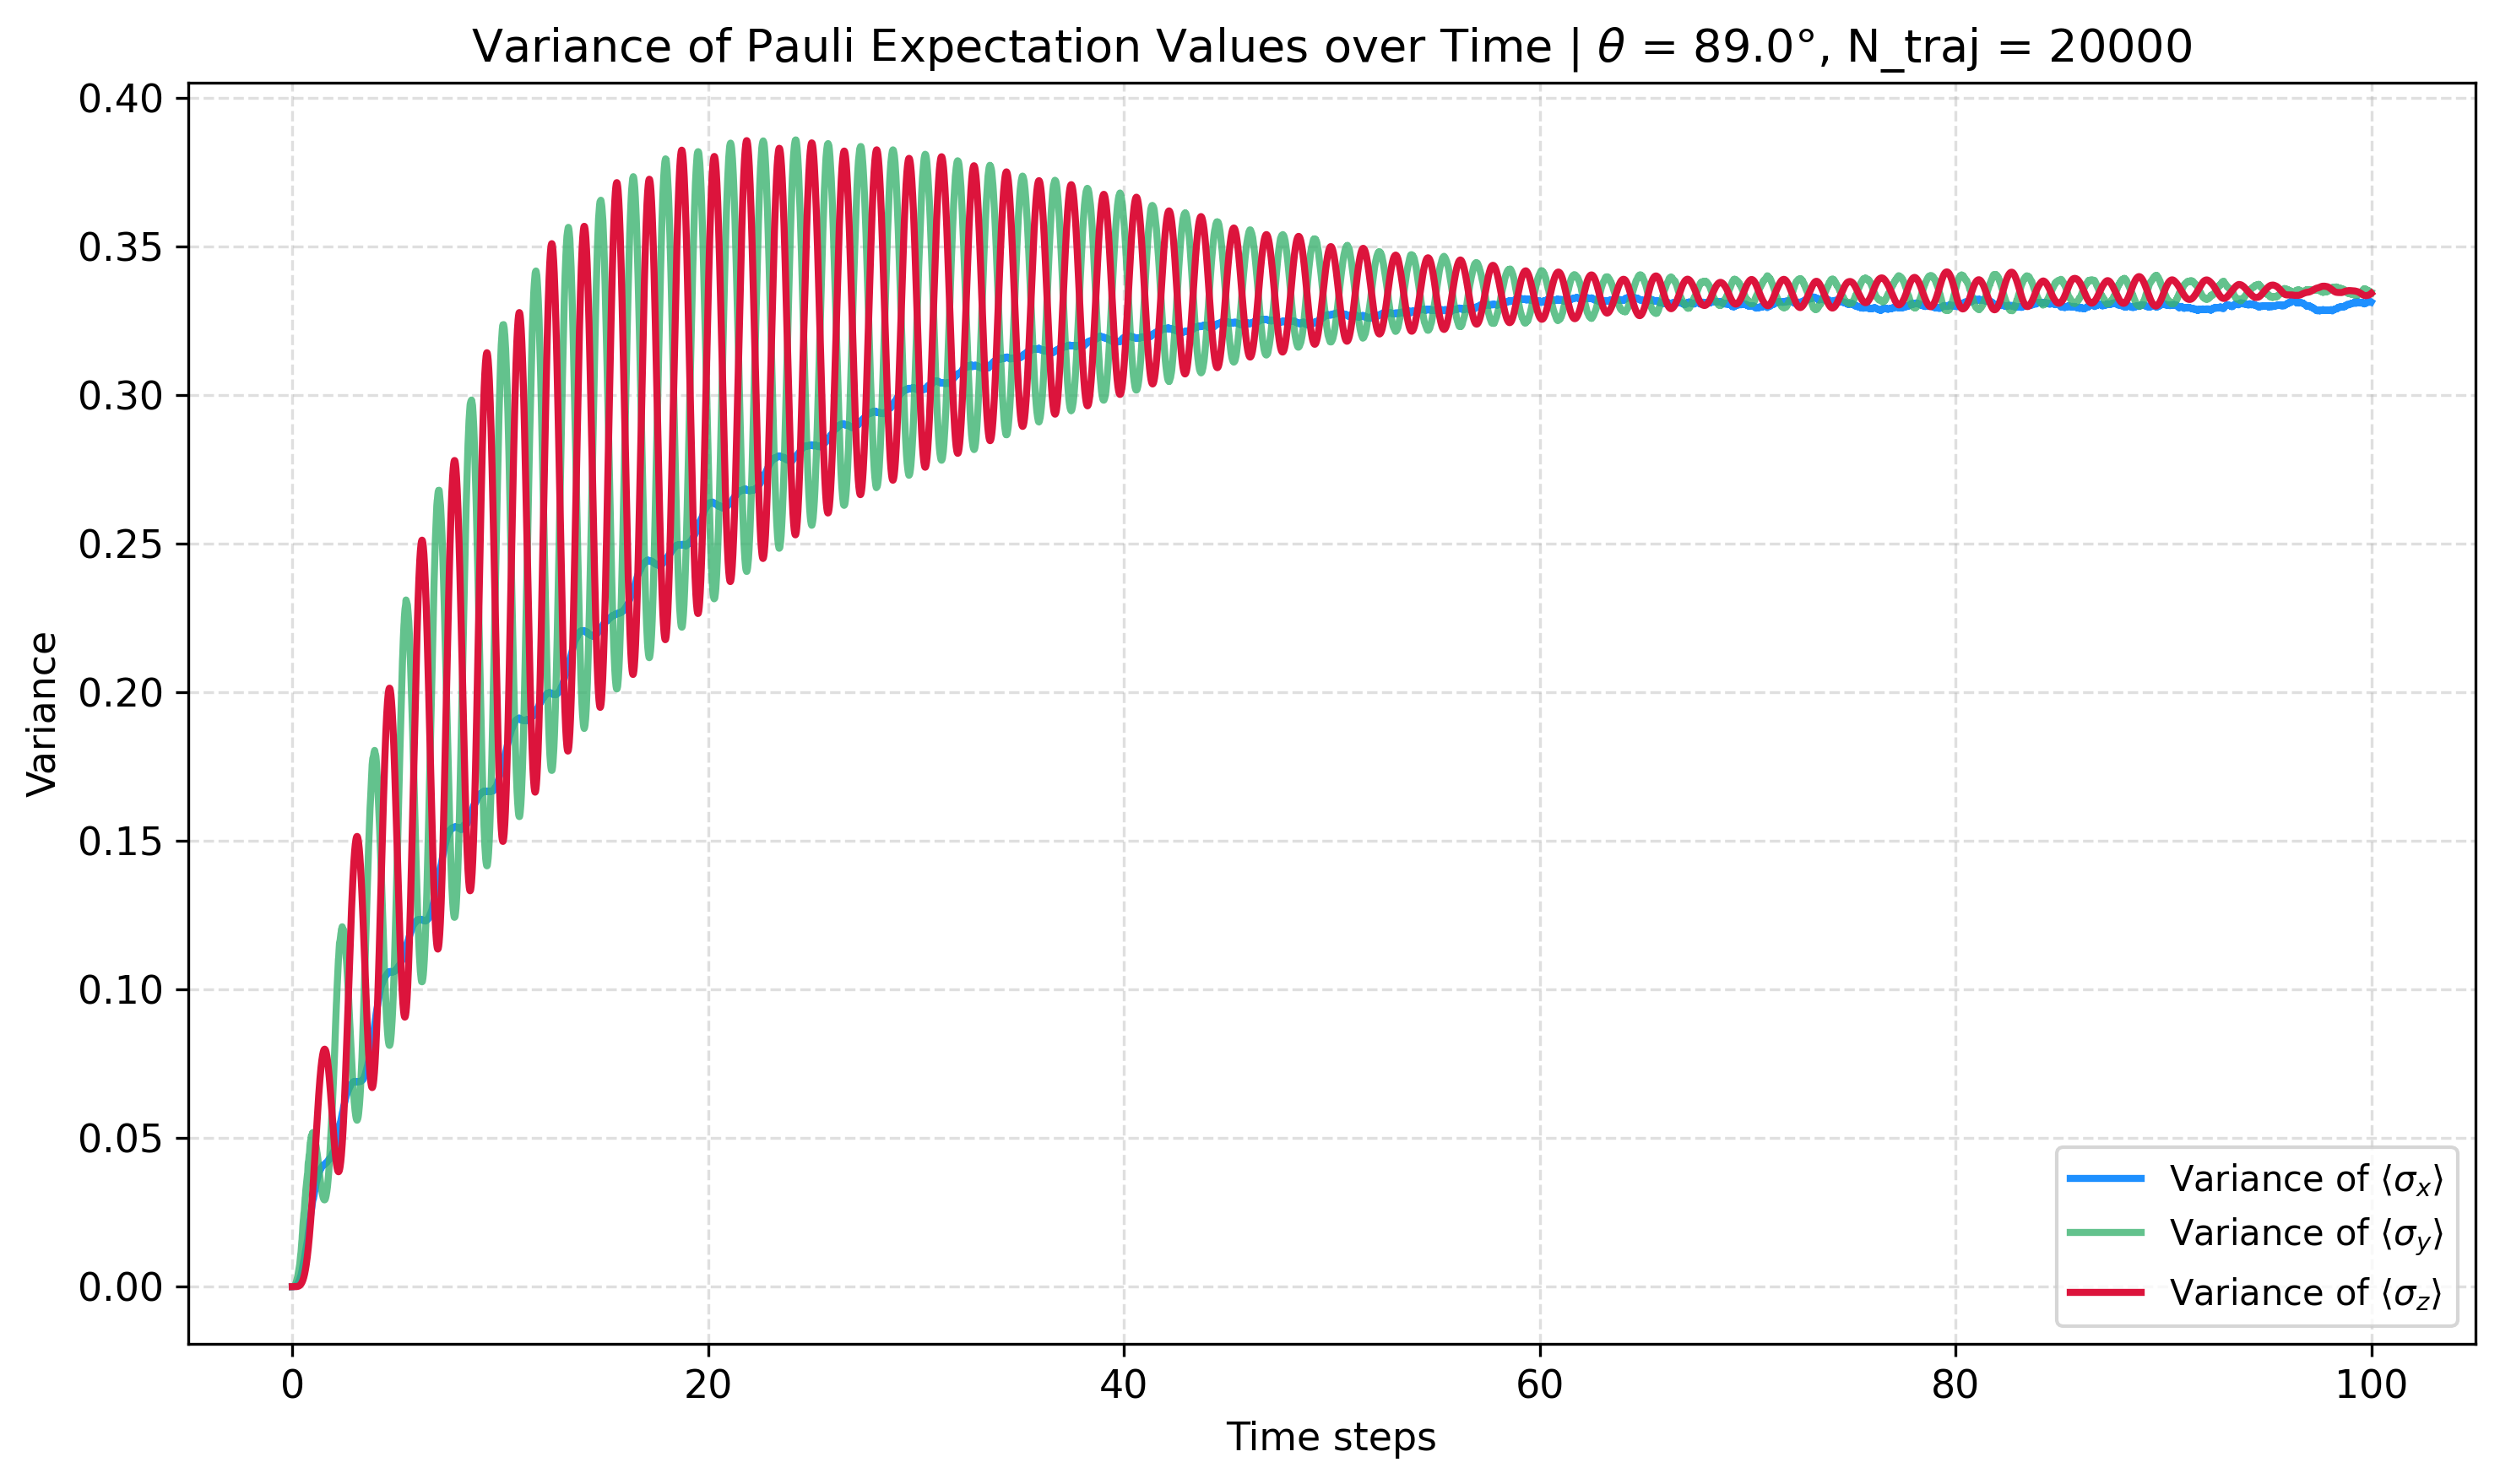
\includegraphics[width=\textwidth]{Variance_Pauli_Theta_1p553343_dt_0p010000_N_traj_20000.png}
		\label{fig:panel_c_Var_Sxyz_89_deg}
		\caption{}
	\end{subfigure}
	\hfill
	\begin{subfigure}[b]{0.40\textwidth}
		\centering
		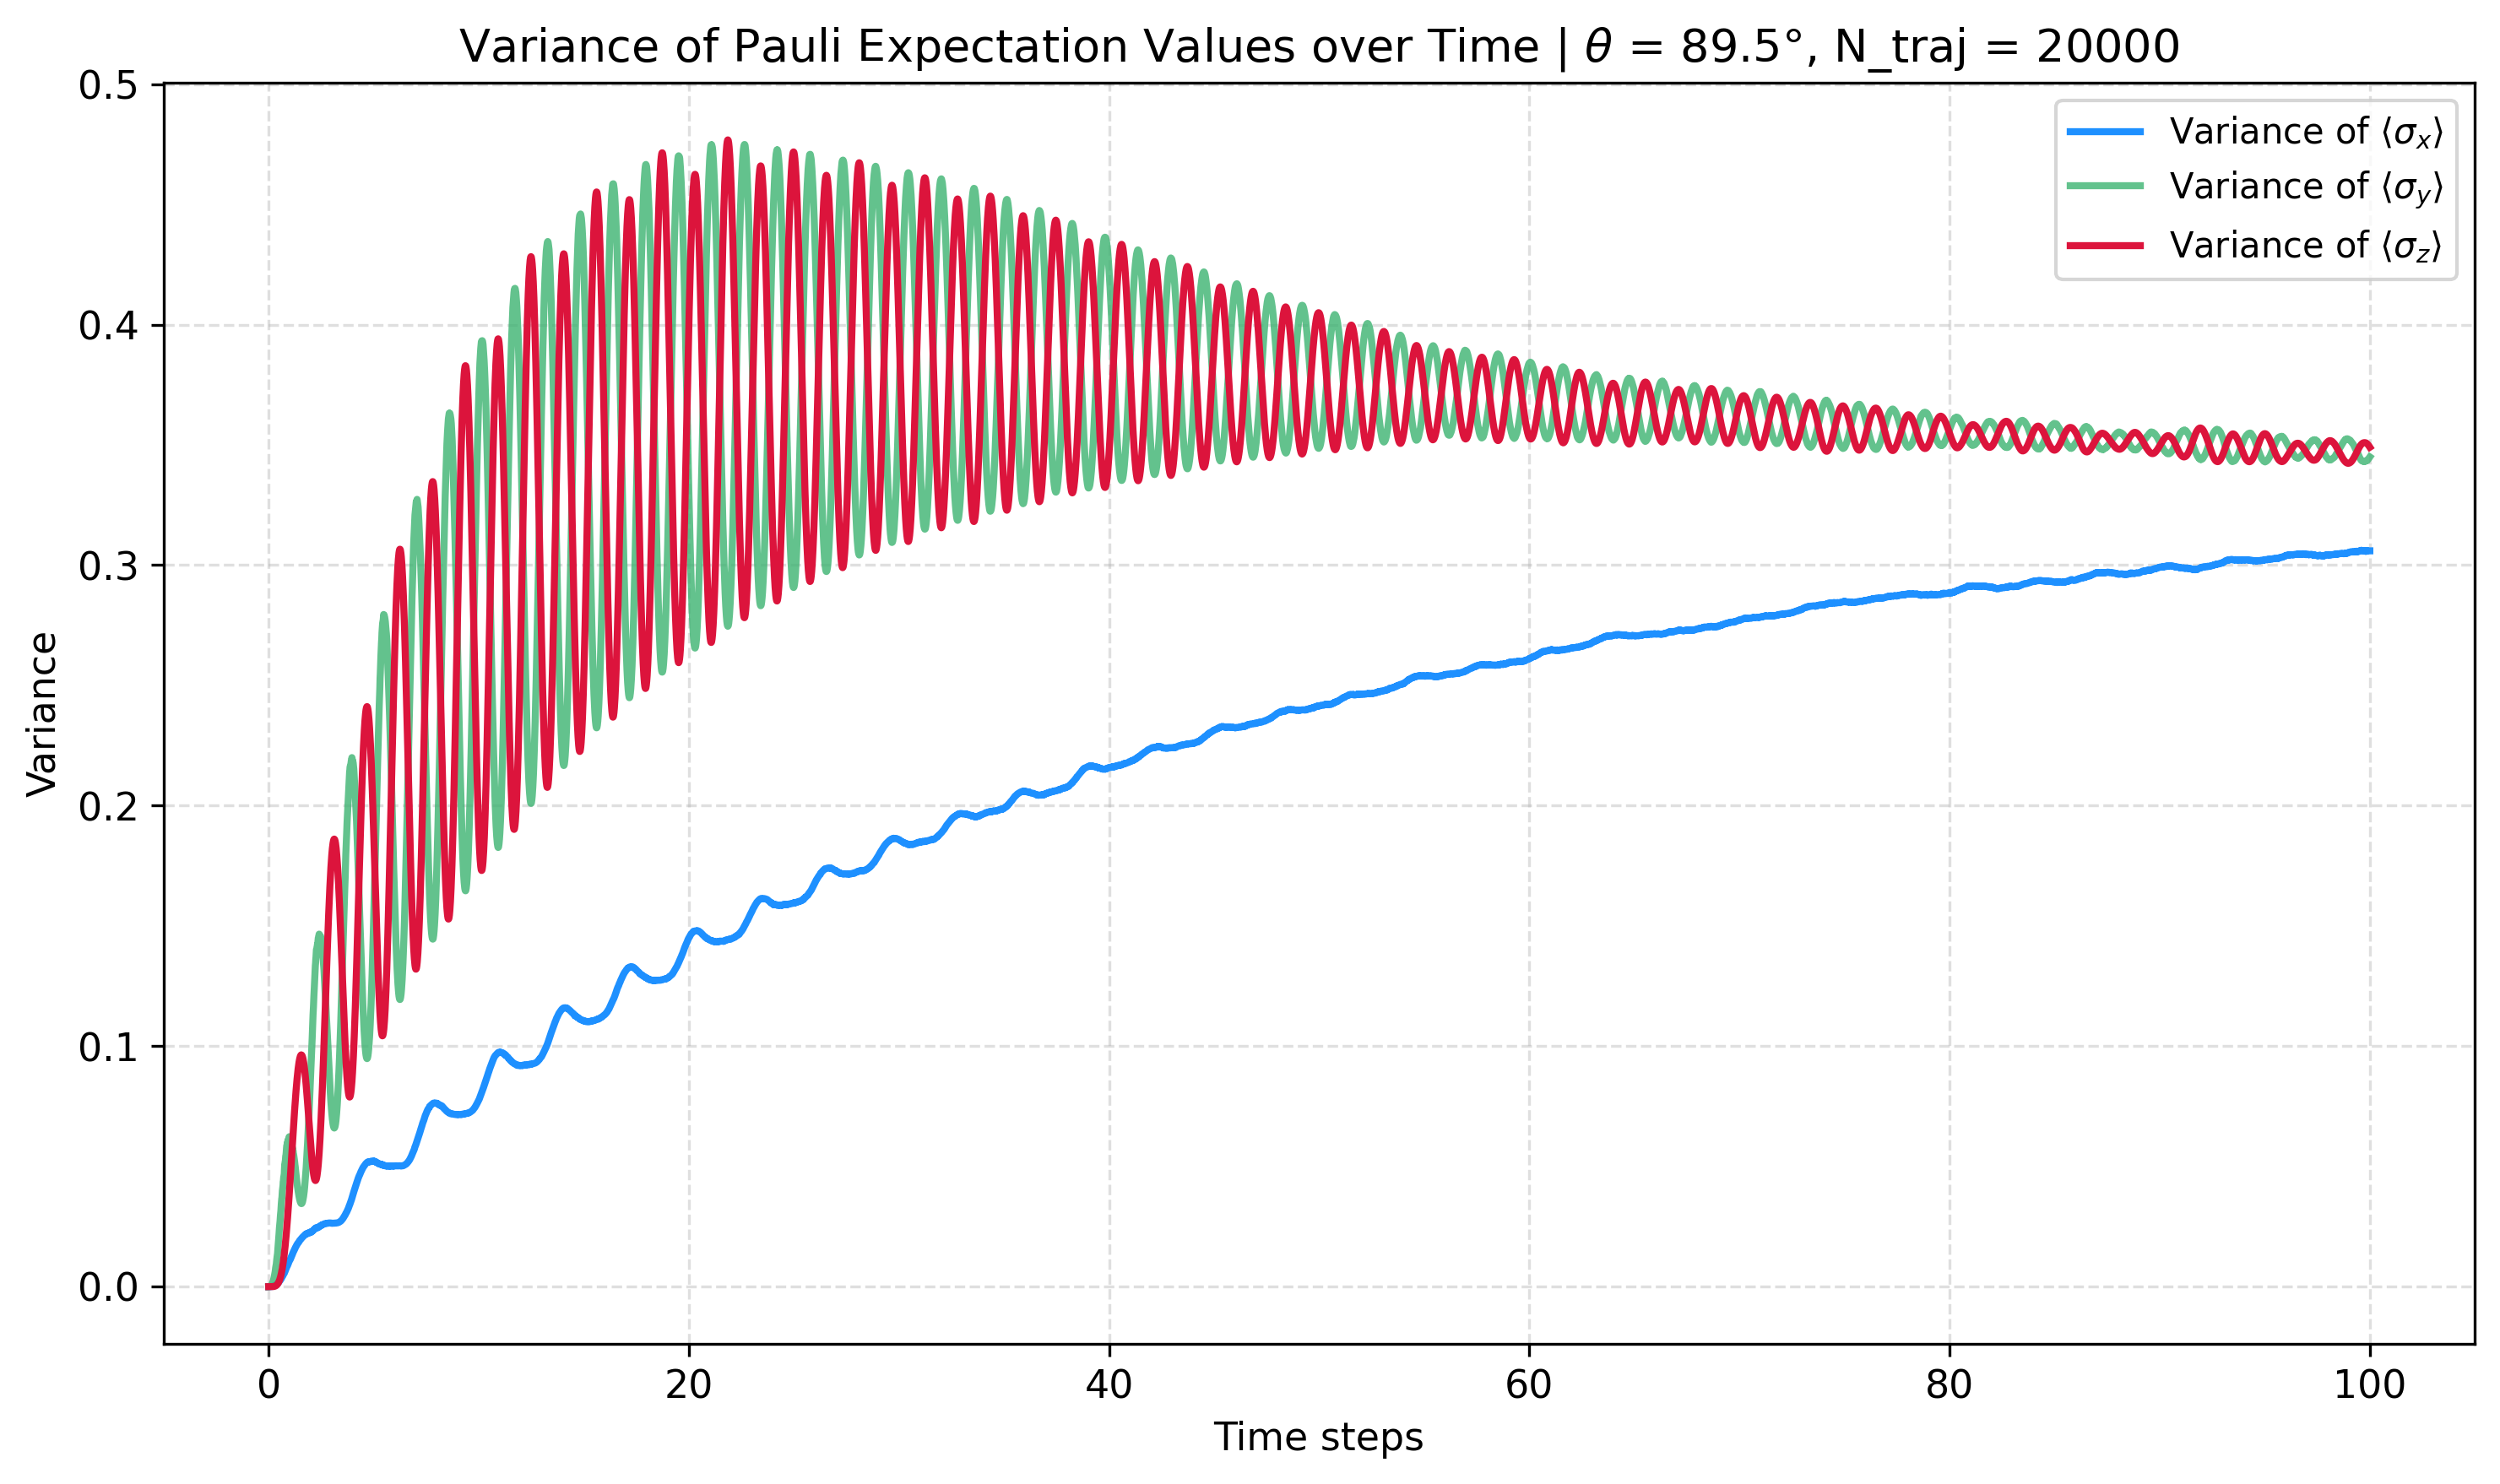
\includegraphics[width=\textwidth]{Variance_Pauli_Theta_1p562070_dt_0p010000_N_traj_20000.png}
		\label{fig:panel_d_Var_Sxyz_89.5_deg}
		\caption{}
	\end{subfigure}
	\caption{Variance over time for the three components of the Bloch vector, calculated for angles close to $ 90^{\circ} $, in particular a) $ \theta = 88.0^{\circ} $, b) $ \theta = 88.5^{\circ} $, c) $ \theta = 89.0^{\circ} $, d) $ \theta = 89.5^{\circ} $ }
\end{figure}
With this plots we can see the effective transition from one limit to the other, that results in a decrease of the Variance of $ \langle \sigma_{x} \rangle $ and an increase in oscillation of $\langle \sigma_y \rangle$ and $\langle \sigma_z \rangle$.

In conclusion, this variance analysis demonstrates that different unraveling schemes exhibit distinct statistical noise profiles. Consequently, depending on the specific observable being evaluated, one can strategically select the mixing angle $\theta$ that minimizes the associated variance. In accordance with the Central Limit Theorem, minimizing this variance directly reduces the statistical error, enabling the achievement of a target precision with a significantly lower number of simulated trajectories and thereby optimizing the overall computational efficiency.

\subsubsection{Singular Value Decomposition}
\label{subsub:SVD_Analysis}
To gain a deeper geometric insight into the statistical distribution of the trajectories, a \textit{Singular Value Decomposition} (SVD) was performed on the matrix containing the Cartesian coordinates of the $N_{Traj}$ Bloch vectors. Geometrically, this procedure is equivalent to a \textit{Principal Component Analysis} (PCA), which models the point cloud of the stochastic trajectories as an enclosing ellipsoid within the Bloch sphere.

The coordinate matrix $X \in \mathbb{R}^{N_{Traj} \times 3}$ containing the Bloch vectors of the $N_{Traj}$ trajectories can be factorized via Singular Value Decomposition (SVD) as:
\begin{equation}
	X = U \Sigma V^T
\end{equation}
where $U \in \mathbb{R}^{N_{Traj} \times N_{Traj}}$ and $V \in \mathbb{R}^{3 \times 3}$ are orthogonal matrices, and $\Sigma \in \mathbb{R}^{N_{Traj} \times 3}$ is a rectangular diagonal matrix. 

Geometrically, the column vectors of $V$ (the right singular vectors) define the mutually orthogonal spatial directions of the principal axes of the ellipsoid bounding the trajectory point cloud, i.e. the principal axes of the covariance matrix associated with the quantum trajectory cloud . The one associated with the first singular value represents the direction where there's the maximal variance, the one associated with the third singular value is the direction of the direction with lowest variance, while the remaining one is just the intermediate orthogonal direction.

The corresponding non-negative diagonal entries of $\Sigma$, known as the singular values $\sigma_k$ (for $k = 1, 2, 3$), represent the lengths of these semi-axes along the principal directions and quantify the geometric spread of the data . Consequently, the squares of the singular values $\sigma_k^2$ are directly proportional to the variance of the data distribution along each respective principal axis.

In the State Diffusion limit ($\theta = 0.0^\circ$), the initial localized point cloud undergoes an isotropic stochastic expansion. As the system evolves, the three singular values asymptotically converge to a single degenerate value. This convergence mathematically demonstrates that the statistical distribution of the trajectories expands uniformly in all spatial directions, ultimately assuming the shape of a perfectly spherical cloud characterized by isotropic variance.

Conversely, in the Quantum Jump limit ($\theta = 90.0^\circ$), the SVD explicitly captures the strong geometric anisotropy of the environmental back-action. Two of the singular values rapidly converge to a higher plateau, quantifying the fast diffusion and thermalization of the trajectories within the yz-plane. Meanwhile, the third singular value, which corresponds to the orthogonal spatial spread along the x-axis, exhibits an extremely slow growth rate. Geometrically, this proves that the statistical ensemble takes the form of a highly flattened, two-dimensional disk-like ellipsoid. This SVD analysis provides a definitive mathematical confirmation of the strongly suppressed out-of-plane variance and the discrepancy in the relaxation timescales discussed in the previous section.

The specific asymptotic values reached by the singular values can be analytically derived from the geometric properties of the Bloch sphere. Let $X$ be the $N_{Traj} \times 3$ coordinate matrix of the ensemble. Because each stochastic trajectory represents a pure state, its Bloch vector satisfies $x_i^2 + y_i^2 + z_i^2 = 1$. Consequently, the trace of the symmetric matrix $X^T X$ is strictly conserved:
\begin{equation}
	\text{Tr}(X^T X) = \sum_{i=1}^{N_{Traj}} (x_i^2 + y_i^2 + z_i^2) = N_{Traj}
\end{equation}
Since the squares of the singular values $\sigma_k^2$ correspond to the eigenvalues of $X^T X$, their sum must equal the total number of trajectories:
\begin{equation}
	\sigma_1^2 + \sigma_2^2 + \sigma_3^2 = N
\end{equation}
Furthermore, the variance along the $k$-th principal axis is related to the singular values by $\text{Var}_k = \frac{\sigma_k^2}{N} - \mu_k^2$, where $\mu_k$ is the ensemble mean. In the long-time limit, assuming the system approaches the completely mixed state ($\vec{\mu} \to 0$), the variance becomes directly proportional to $\sigma_k^2$.

In the State Diffusion limit ($\theta = 0.0^\circ$), the statistical noise is fully isotropic in three dimensions, implying $\sigma_1 = \sigma_2 = \sigma_3$. Applying the trace conservation law yields $3\sigma^2 = N_{Traj}$, from which we obtain $\sigma = \sqrt{N/3}$. For $N_{Traj} = 10000$, this results in an asymptotic plateau of $\sigma \approx 57.73$, perfectly matching the numerical simulation.

Conversely, in the Quantum Jump limit ($\theta = 90.0^\circ$), the dynamics is heavily constrained to the yz-plane, suppressing the out-of-plane variance such that $\sigma_3 \approx 0$. The isotropic diffusion in the remaining two dimensions implies $\sigma_1 = \sigma_2$. The trace conservation law then reduces to $2\sigma^2 = N$, yielding $\sigma = \sqrt{N_{Traj}/2}$. For $N_{Traj} = 10000$, this analytically predicts the observed plateau at $\sigma \approx 70.71$.

In the State Diffusion limit ($\theta = 0^\circ$), the trajectory ellipsoid undergoes an isotropic expansion. The three normalized singular values converge asymptotically to the same value, $1/\sqrt{3} \approx 0.577$. This indicates that the stochastic diffusion uniformly explores the allowed Bloch space, ultimately forming a perfect sphere.

Conversely, in the Quantum Jump limit ($\theta = 90^\circ$), the evolution is strongly anisotropic. One of the principal axes is consistently suppressed, which forces the dispersion of the trajectories to collapse onto a two-dimensional manifold, effectively forming a disk. This geometric and dimensional collapse is a direct visual manifestation of the confinement imposed by the jump operators on the quantum coherences of the system.

\newpage

\section{General Treatment for Collisional Methods}
\label{sec:General_Treatment_for_Collisional Methods}

In this section we try to define a general definition and treatment for \textit{Collisional Methods} model, defining the \textit{Collisional Hamiltonian} $ \mathcal{H}_{Coll} $, the related Evolution Operator $ \mathcal{U}_{Coll} $ and the associated \textit{Kraus Operators} $ \mathcal{K} $; we will define a general formalism that allows to create different $ \mathcal{K} $, associated to different Ancilla's basis for the measurement, that generates different \textit{Unraveling Scheme}. \newline
Most of this section in based on the article from Ciccarello\cite{ciccarelloQuantumCollisionModels2022}.

\subsection{Hamiltonian Definition}
The generic Hamiltonian for a Collisional Model describes the mutual exchange in energy and information between System and environment (represented by the Ancilla); since the model have to reproduce the QME dynamics it's plausible to usa the same Jump Operator on the System, while since the Ancilla is a qubit we can assume two possible evolution of its state, given by the operators : $ \sigma_{-} = \begin{pmatrix} 0 & 1 \\ 0 & 0 \end{pmatrix} $ and $ \sigma_{+} = \begin{pmatrix} 0 & 0 \\ 1 & 0 \end{pmatrix} $, that represent the relaxation to the ground state $ \ket{0_{a}} = \begin{pmatrix} 1 \\ 0 \end{pmatrix} $ and the excitation to $ \ket{1_{a}} = \begin{pmatrix} 0 \\ 1 \end{pmatrix} $. \newline
With this elements we can compose the \textit{Collisional Hamiltonian}, as reported in Cattaneo's article\cite{cattaneoCollisionModelsCan2021} : 
\begin{equation}
	\mathcal{H}_{Coll} = c_{k} \left(\mathcal{L}_{k} \otimes \sigma_{+}^{a} + \mathcal{L}_{k}^{\dagger} \otimes \sigma_{-}^{a} \right)
	\label{eq:general_H_CM}
\end{equation}
with $ c_{k} = \sqrt{\frac{\gamma_{k}}{\Delta t}} $ the coefficient that defines the Intensity of the Collision, $ \mathcal{L}_{k} $ the Lindblad Jump Operator, defining the $ k-th $ dissipation channel acting on the System, while $ \sigma_{-}^{a} $ and $ \sigma_{+}^{a} $ act on the Ancilla. 

This is the most general form of the \textit{Collisional Hamiltonian} that can represent any CPTP QME; by choosing different Ancilla's initial state one can model the action of the operator, i.e. with $ \ket{\phi_{a}} = \ket{0_{a}} $ the second term in Eq.\ref{eq:general_H_CM} vanishes. \newline
In general we can take $ \ket{\phi_{a}} = \sqrt{p_{a}} \ket{0_{a}} + \sqrt{1 - p_{a }} \ket{1_{a}} $.

\subsection{Unitary Evolution Operator}
Once we defined $ \mathcal{H}_{Coll} $ we can build up the \textit{Unitary Evolution Operator} as : 
\begin{equation}
	\mathcal{U}_{Coll} \left( \Delta t \right) = \exp \left( -i \mathcal{H}_{Coll} \Delta t \right) = \sum_{m}^{\infty}{\frac{\left( -i \mathcal{H}_{Coll} \Delta t \right)^{m}}{m!}}
\end{equation}
Separating and analyzing separately the even and odd term we obtain: 
\begin{align}
	\sum_{m=0}^{\infty}{ \frac{\left( -i \mathcal{H}_{Coll} \Delta t \right)^{2m}}{(2m)!} } &= \sum_{m=0}^{\infty}{ \frac{\left( -i c \Delta t \right)^{2m}}{(2m)!} \left( \mathcal{L}_{k} \otimes \sigma_{+}^{a} + \mathcal{L}_{k}^{\dagger} \otimes \sigma_{-}^{a} \right)^{2m}} \notag \\
	&= \sum_{m=0}^{\infty}{ \frac{\left( -i c \Delta t \right)^{2m}}{(2m)!} \left( \sqrt{\mathcal{L}_{k} \mathcal{L}_{k}^{\dagger} }\right)^{2m} \otimes P_{11}^{a} } + \sum_{m=0}^{\infty}{ \frac{\left( -i c \Delta t \right)^{2m}}{(2m)!} \left( \sqrt{\mathcal{L}_{k}^{\dagger} \mathcal{L}_{k} }\right)^{2m} \otimes P_{00}^{a} } \notag \\
	&= \cos{\left(c \Delta t \sqrt{\mathcal{L}_{k} \mathcal{L}_{k}^{\dagger} }\right) } \otimes P_{11}^{a} + \cos{\left(c \Delta t \sqrt{\mathcal{L}_{k}^{\dagger} \mathcal{L}_{k} } \right) } \otimes P_{00}^{a}
\end{align} 

with $P_{00}^{a} = \ket{0_{a}} \bra{0_{a}} = \sigma_{-}\sigma_{+}$ and $ P_{11}^{a} = \ket{1_{a}} \bra{1_{a}} = \sigma_{+}\sigma_{-}  $

\begin{align}
	\sum_{m=0}^{\infty}{ \frac{\left( -i \mathcal{H}_{Coll} \Delta t \right)^{2m+1}}{(2m+1)!} } &= \sum_{m=0}^{\infty}{ \frac{\left( -i c \Delta t \right)^{2m+1}}{(2m+1)!} \left( \mathcal{L}_{k} \otimes \sigma_{+}^{a} + \mathcal{L}_{k}^{\dagger} \otimes \sigma_{-}^{a} \right)^{2m+1}} \notag \\
	&= \left(\sum_{m=0}^{\infty}{\frac{\left( -i c \Delta t \right)^{2m+1}}{(2m+1)!} \frac{\left( \sqrt{\mathcal{L}_{k} \mathcal{L}_{k}^{\dagger} }\right)^{2m+1}}{\sqrt{\mathcal{L}_{k} \mathcal{L}_{k}^{\dagger} }}} \right) \mathcal{L}_{k} \otimes \sigma_{+}^{a} \notag \\
	&+ \left(\sum_{m=0}^{\infty}{\frac{\left( -i c \Delta t \right)^{2m+1}}{(2m+1)!} \frac{\left( \sqrt{\mathcal{L}_{k}^{\dagger} \mathcal{L}_{k} }\right)^{2m+1}}{\sqrt{\mathcal{L}_{k}^{\dagger} \mathcal{L}_{k} }}} \right) \mathcal{L}_{k}^{\dagger} \otimes \sigma_{-}^{a} \notag \\
	&= -i \sin \left( c \Delta t \sqrt{\mathcal{L}_{k} \mathcal{L}_{k}^{\dagger}} \right) \frac{\mathcal{L}_{k} \otimes \sigma_{+}^{a}}{\sqrt{\mathcal{L}_{k} \mathcal{L}_{k}^{\dagger}}} -i \sin \left( c \Delta t \sqrt{\mathcal{L}_{k}^{\dagger} \mathcal{L}_{k}} \right) \frac{\mathcal{L}_{k}^{\dagger} \otimes \sigma_{-}^{a}}{\sqrt{\mathcal{L}_{k}^{\dagger} \mathcal{L}_{k}}} 
\end{align}
The operator is obtained by summing the even (cosine) and odd (sine) series
\begin{align}
	U &= \cos{\left(c \Delta t \sqrt{\mathcal{L}_{k} \mathcal{L}_{k}^{\dagger} }\right) } \otimes P_{11}^{a} + \cos{\left(c \Delta t \sqrt{\mathcal{L}_{k}^{\dagger} \mathcal{L}_{k} } \right) } \otimes P_{00}^{a} \notag \\
	&\quad -i \sin \left( c \Delta t \sqrt{\mathcal{L}_{k} \mathcal{L}_{k}^{\dagger}} \right) \frac{\mathcal{L}_{k} \otimes \sigma_{+}^{a}}{\sqrt{\mathcal{L}_{k} \mathcal{L}_{k}^{\dagger}}} -i \sin \left( c \Delta t \sqrt{\mathcal{L}_{k}^{\dagger} \mathcal{L}_{k}} \right) \frac{\mathcal{L}_{k}^{\dagger} \otimes \sigma_{-}^{a}}{\sqrt{\mathcal{L}_{k}^{\dagger} \mathcal{L}_{k}}}
\end{align}

\subsection{Kraus Operators}
Once we defined the Evolution Operator, we can use it to calculate the \textit{Kraus Operators} defined in the \textit{Petruccione} as :
\begin{align}
	\rho_{S} \left(t\right) &= \mathcal{V}\left(t\right) \rho_{S} \left(0\right) = Tr_{B} \Big\{ \mathcal{U}\left(t, t_0\right) \Big[ \rho_{S} \otimes \rho_{B} \Big] \mathcal{U}^{\dagger}\left(t, t_0\right) \Big\} \\
	&\left( \rho_{B} = \sum_{\alpha}{\lambda_{\alpha} \ket{\varphi_{\alpha}} \bra{\varphi_{\alpha}}} \quad \text{and} \quad Tr_{B} = \sum_{\beta}{\bra{\varphi_{\beta}} \dots \ket{\varphi_{\beta}}} \right) \notag \\
	&= \sum_{\alpha}{\sum_{\beta}{\lambda_{\alpha}\bra{\varphi_{\beta}} \mathcal{U}\left(t, t_0\right) \left[ \rho_{S} \otimes \ket{\varphi_{\alpha}} \bra{\varphi_{\alpha}} \right]  \mathcal{U}^{\dagger}\left(t, t_0\right) \ket{\varphi_{\beta}} }} \notag \\
	&= \sum_{\alpha, \beta}{ \mathcal{W}_{\alpha, \beta} \left(t\right) \rho_{S} \mathcal{W}^{\dagger}_{\alpha, \beta} \left(t\right) }
	\label{eq:dynamical_map_kraus_operators}
\end{align}
where $ \mathcal{W}_{\alpha, \beta} \left(t\right) $ are operators that act on the \textit{wf} of the system solely, defining the evolution conditioned by the measurement of the bath state; this operators take the form :
\begin{equation}
	\mathcal{W}_{\alpha, \beta} \left(t\right) = \sqrt{\lambda_{\alpha}} \bra{\varphi_{\beta}}  \mathcal{U}\left(t, t_0\right) \ket{\varphi_{\alpha}}
	\label{eq:general_kraus_operators}
\end{equation}
The set of operators $\{ \mathcal{W}_{\alpha, \beta} \}$ formally constitutes a set of \textit{Kraus Operators}, where the standard single Kraus index is represented by the pair $(\alpha, \beta)$. Since they satisfy the completeness relation $\sum_{\alpha, \beta} \mathcal{W}_{\alpha, \beta}^\dagger \mathcal{W}_{\alpha, \beta} = \mathbb{I}_S$, they guarantee a Completely Positive and Trace-Preserving (CPTP) map.

We use as $ \lambda_{\beta} $ and $ \ket{\varphi_{\beta}} $ the eigenvalue and eigenstate obtained with the spectral decomposition of the initial environment density matrix.
First, we define the pure coherent state of the ancilla and calculate its associated density matrix:
\begin{align}
	\ket{\phi_a} &= \sqrt{p} \ket{0_a} + \sqrt{1-p} \ket{1_a} \\
	\rho_a &= \ket{\phi_a}\bra{\phi_a} \notag \\
	&= p \ket{0_a}\bra{0_a} + \sqrt{p(1-p)} \ket{0_a}\bra{1_a} + \sqrt{p(1-p)} \ket{1_a}\bra{0_a} + (1-p) \ket{1_a}\bra{1_a}
\end{align}

Since the ancilla is in a perfectly pure state, the spectral decomposition of its density matrix yields only one non-zero eigenvalue ($\lambda_1 = 1$) associated with the eigenvector $\ket{\phi_a}$. The other eigenvalue ($\lambda_2 = 0$) is associated with the orthogonal state $\ket{\phi_a^\perp}$:
\begin{align}
	\rho_a &= 1 \cdot \ket{\phi_a}\bra{\phi_a} + 0 \cdot \ket{\phi_a^\perp}\bra{\phi_a^\perp}
\end{align}

The resulting Kraus operators are derived exclusively using the non-zero eigenvalue ($\lambda = 1$). The general formula $\mathcal{K}_i = \sqrt{\lambda} \bra{i_a} U \ket{\lambda}$ therefore reduces to simply evaluating the matrix elements $\bra{i_a} U \ket{\phi_a}$:
\begin{align}
	\mathcal{K}_{0} &= \bra{0_a} U \ket{\phi_a} \notag \\
	&= \sqrt{p} \cos{\left(c \Delta t \sqrt{\mathcal{L}_{k}^{\dagger} \mathcal{L}_{k} } \right)} -i \sqrt{1-p} \sin{\left( c \Delta t \sqrt{\mathcal{L}_{k}^{\dagger} \mathcal{L}_{k}} \right)} \frac{\mathcal{L}_{k}^{\dagger}}{\sqrt{\mathcal{L}_{k}^{\dagger} \mathcal{L}_{k}}} \\
	\mathcal{K}_{1} &= \bra{1_a} U \ket{\phi_a} \notag \\
	&= -i \sqrt{p} \sin{\left( c \Delta t \sqrt{\mathcal{L}_{k} \mathcal{L}_{k}^{\dagger}} \right)} \frac{\mathcal{L}_{k}}{\sqrt{\mathcal{L}_{k} \mathcal{L}_{k}^{\dagger}}} + \sqrt{1-p} \cos{\left(c \Delta t \sqrt{\mathcal{L}_{k} \mathcal{L}_{k}^{\dagger} }\right)}
\end{align}

Alternatively, if we consider the case where the ancilla is strictly initialized in its ground state, the wavefunction and its corresponding density matrix are simply:
\begin{align}
	\ket{\psi_a} &= \ket{0_a} \\
	\rho_a &= \ket{0_a}\bra{0_a}
\end{align}

This density matrix is already in its diagonal form, possessing a single non-zero eigenvalue ($\lambda = 1$) associated with the state $\ket{0_a}$. By evaluating the general formula $\mathcal{K}_i = \bra{i_a} U \ket{0_a}$, the evolution of the system is completely described by just two specific Kraus operators:
\begin{align}
	\mathcal{K}_{0} &= \bra{0_a} U \ket{0_a} \notag \\
	&= \cos{\left(c \Delta t \sqrt{\mathcal{L}_{k}^{\dagger} \mathcal{L}_{k} } \right)} \\
	\mathcal{K}_{1} &= \bra{1_a} U \ket{0_a} \notag \\
	&= -i \sin{\left( c \Delta t \sqrt{\mathcal{L}_{k} \mathcal{L}_{k}^{\dagger}} \right)} \frac{\mathcal{L}_{k}}{\sqrt{\mathcal{L}_{k} \mathcal{L}_{k}^{\dagger}}}
\end{align}

To evaluate trigonometric functions of operators, a formal and highly effective approach is to expand them using their Taylor series. Defining the effective angle $\theta = c \Delta t$ and a generic positive semi-definite operator $A = \sqrt{\mathcal{L}_{k}^{\dagger} \mathcal{L}_{k}}$ (or $A = \sqrt{\mathcal{L}_{k} \mathcal{L}_{k}^{\dagger}}$ for the sine operator), the general expansions are:
\begin{align}
	\cos(\theta A) &= \sum_{n=0}^{\infty} \frac{(-1)^n}{(2n)!} (\theta A)^{2n} = \mathbb{I} - \frac{\theta^2}{2!} A^2 + \frac{\theta^4}{4!} A^4 - \dots \\
	\sin(\theta A) &= \sum_{n=0}^{\infty} \frac{(-1)^n}{(2n+1)!} (\theta A)^{2n+1} = \theta A - \frac{\theta^3}{3!} A^3 + \frac{\theta^5}{5!} A^5 - \dots
\end{align}

This series expansion approach leads to massive simplifications when dealing with operators that possess specific algebraic properties. We can examine two fundamental physical scenarios.

First, consider a pure dephasing process where $\mathcal{L}_{k} = \sigma_{z}$. The product is $\mathcal{L}_{k}^{\dagger} \mathcal{L}_{k} = \sigma_{z}^2 = \mathbb{I}$. Because every power of the identity matrix is the identity itself ($\mathbb{I}^n = \mathbb{I}$), the infinite series collapse directly into scalar trigonometric functions multiplying the identity:
\begin{align}
	\cos(\theta \mathbb{I}) &= \mathbb{I} \sum_{n=0}^{\infty} \frac{(-1)^n}{(2n)!} \theta^{2n} = \cos(\theta) \mathbb{I} \\
	\sin(\theta \mathbb{I}) &= \mathbb{I} \sum_{n=0}^{\infty} \frac{(-1)^n}{(2n+1)!} \theta^{2n+1} = \sin(\theta) \mathbb{I}
\end{align}
Applying these to our equations for an ancilla initialized in the ground state, the effective Kraus operators for the pure dephasing channel become:
\begin{align}
	\mathcal{K}_{0} &= \cos(c \Delta t) \mathbb{I} \\
	\mathcal{K}_{1} &= -i \sin(c \Delta t) \sigma_{z}
\end{align}

Second, consider the amplitude damping channel where $\mathcal{L}_{k} = \sigma_{-}$. The product $\mathcal{L}_{k}^{\dagger} \mathcal{L}_{k} = \sigma_{+} \sigma_{-}$ acts as a projection operator $P$. Since projectors are idempotent ($P^n = P$ for any $n \ge 1$), the infinite series collapses into simple closed forms. Recalling that $P^0 = \mathbb{I}$, we obtain:
\begin{align}
	\cos(\theta P) &= \mathbb{I} - P + P \sum_{n=0}^{\infty} \frac{(-1)^n}{(2n)!} \theta^{2n} = \mathbb{I} - P + \cos(\theta) P \\
	\sin(\theta P) &= P \sum_{n=0}^{\infty} \frac{(-1)^n}{(2n+1)!} \theta^{2n+1} = \sin(\theta) P
\end{align}
The corresponding effective Kraus operators for the amplitude damping channel simplify beautifully to:
\begin{align}
	\mathcal{K}_{0} &= \mathbb{I} - \sigma_{+}\sigma_{-} + \cos(c \Delta t) \sigma_{+}\sigma_{-} \\
	\mathcal{K}_{1} &= -i \sin(c \Delta t) \sigma_{-}
\end{align}

However, for a generic arbitrary operator $\mathcal{L}_{k}$ lacking such idempotency or involution, the Taylor series does not yield a simple factored form. In the general case, we must rely on the spectral decomposition theorem. By diagonalizing the Hermitian operator $\mathcal{L}_{k}^{\dagger} \mathcal{L}_{k}$ to find its eigenvalues $\lambda_m$ and eigenvectors $\ket{m}$, we can evaluate the trigonometric functions directly on its spectrum:
\begin{align}
	\mathcal{L}_{k}^{\dagger} \mathcal{L}_{k} &= \sum_{m} \lambda_m \ket{m}\bra{m} \\
	\cos\left(c \Delta t \sqrt{\mathcal{L}_{k}^{\dagger} \mathcal{L}_{k}}\right) &= \sum_{m} \cos\left(c \Delta t \sqrt{\lambda_m}\right) \ket{m}\bra{m} \\
	\sin\left(c \Delta t \sqrt{\mathcal{L}_{k}^{\dagger} \mathcal{L}_{k}}\right) &= \sum_{m} \sin\left(c \Delta t \sqrt{\lambda_m}\right) \ket{m}\bra{m}
\end{align}

This spectral formulation provides a rigorous pathway to calculate the matrix representation of the Kraus operators numerically or analytically, regardless of the complexity of $\mathcal{L}_{k}$.

\subsection{Generating different Kraus Operators}
We can demonstrate that we can generate different \textit{Kraus Operators} by changing the basis used for the trace : 
\begin{align}
	\rho_{S} \left(t\right) &= \mathcal{V}\left(t\right) \rho_{S} \left(0\right) = Tr_{B} \Big\{ \mathcal{U}\left(t, t_0\right) \Big[ \rho_{S} \otimes \rho_{B} \Big] \mathcal{U}^{\dagger}\left(t, t_0\right) \Big\} \\
	&=\sum_{\alpha}{\lambda_{\alpha} {\sum_{\beta} \bra{\varphi_{\beta}} \mathcal{U}\left(t, t_0\right) \left[ \rho_{S} \otimes \ket{\varphi_{\alpha}} \bra{\varphi_{\alpha}} \right]  \mathcal{U}^{\dagger}\left(t, t_0\right) \ket{\varphi_{\beta}} }} \notag \\
	&\left( \text{using the \textit{Identity} definition} \quad \mathbb{I} = \sum_{\gamma}{\ket{\eta_{\gamma}} \bra{\eta_{\gamma}} } \right) \notag \\
	&=\sum_{\alpha} {\lambda_{\alpha} {\sum_{\beta} \bra{\varphi_{\beta}} \left( \sum_{\gamma}{\ket{\eta_{\gamma}} \bra{\eta_{\gamma}} } \right) \mathcal{U}\left(t, t_0\right) \left[ \rho_{S} \otimes \ket{\varphi_{\alpha}} \bra{\varphi_{\alpha}} \right]  \mathcal{U}^{\dagger}\left(t, t_0\right) \ket{\varphi_{\beta}} }} \notag \\
	&=\sum_{\alpha} {\lambda_{\alpha} {\sum_{\beta} \sum_{\gamma} \bra{\varphi_{\beta}} \ket{\eta_{\gamma}} \bra{\eta_{\gamma}} \mathcal{U}\left(t, t_0\right) \left[ \rho_{S} \otimes \ket{\varphi_{\alpha}} \bra{\varphi_{\alpha}} \right]  \mathcal{U}^{\dagger}\left(t, t_0\right) \ket{\varphi_{\beta}} }} \notag \\
	&=\sum_{\alpha} {\lambda_{\alpha} {\sum_{\beta} \sum_{\gamma} \bra{\eta_{\gamma}} \mathcal{U}\left(t, t_0\right) \left[ \rho_{S} \otimes \ket{\varphi_{\alpha}} \bra{\varphi_{\alpha}} \right]  \mathcal{U}^{\dagger}\left(t, t_0\right) \ket{\varphi_{\beta}} \bra{\varphi_{\beta}} \ket{\eta_{\gamma}} }} \notag \\
	&\left( \text{and again} \quad \mathbb{I} = \sum_{\beta}{\ket{\varphi_{\beta}} \bra{\varphi_{\beta}} } \right) \notag \\
	&=\sum_{\alpha}{\lambda_{\alpha} {\sum_{\gamma} \bra{\eta_{\gamma}} \mathcal{U}\left(t, t_0\right) \left[ \rho_{S} \otimes \ket{\varphi_{\alpha}} \bra{\varphi_{\alpha}} \right]  \mathcal{U}^{\dagger}\left(t, t_0\right) \ket{\eta_{\gamma}} }} \notag \\
\end{align}
So that we obtain new \textit{Kraus Operators} but using a different base for the Ancilla Trace  : 
\begin{equation}
	\mathcal{W}_{\alpha, \gamma} \left(t\right) = \sqrt{\lambda_{\alpha}} \bra{\eta_{\gamma}}  \mathcal{U}\left(t, t_0\right) \ket{\varphi_{\alpha}}
\end{equation}
Using from the original definition of the \textit{Kraus Operators} and again using the \textit{Identity} definition we see that : 
\begin{align}
	\mathcal{W}_{\alpha, \gamma} \left(t\right) &= \sqrt{\lambda_{\alpha}} \bra{\eta_{\gamma}} \mathcal{U}\left(t, t_0\right) \ket{\varphi_{\alpha}} \notag \\
	&= \sqrt{\lambda_{\alpha}} \bra{\eta_{\gamma}} \left( \sum_{\beta} \ket{\varphi_{\beta}} \bra{\varphi_{\beta}} \right) \mathcal{U}\left(t, t_0\right) \ket{\varphi_{\alpha}} \notag \\
	&= \sqrt{\lambda_{\alpha}} \sum_{\beta} \bra{\eta_{\gamma}} \ket{\varphi_{\beta}} \bra{\varphi_{\beta}} \mathcal{U}\left(t, t_0\right) \ket{\varphi_{\alpha}} = \sum_{\beta} \mathcal{W}_{\alpha, \beta} \left(t\right)
\end{align}
We can reformulate the change in the Ancilla Trace basis using a unitary transformation : 
\begin{gather}
	\ket{\eta_{\gamma}} = V \ket{\varphi_{\gamma}} \quad \text{and} \quad \bra{\eta_{\gamma}} = \bra{\varphi_{\gamma}} V^{\dagger} \\
	\text{with} \quad V = \sum_{\gamma}{\ket{\eta_{\gamma}} \bra{\phi_{\gamma}}}
\end{gather}
so that : 
\begin{align}
	\mathcal{W}_{\alpha, \gamma} \left(t\right) &= \sqrt{\lambda_{\alpha}} \bra{\eta_{\gamma}} \mathcal{U}\left(t, t_0\right) \ket{\varphi_{\alpha}} \notag \\
	&= \sqrt{\lambda_{\alpha}} \bra{\varphi_{\gamma}} V^{\dagger} \mathcal{U}\left(t, t_0\right) \ket{\varphi_{\alpha}} \notag \\
	&= \sqrt{\lambda_{\alpha}} \bra{\varphi_{\gamma}} V^{\dagger} \left( \sum_{\beta} \ket{\varphi_{\beta}} \bra{\varphi_{\beta}} \right) \mathcal{U}\left(t, t_0\right) \ket{\varphi_{\alpha}} \notag \\
	&= \sum_{\beta} \bra{\varphi_{\gamma}} V^{\dagger} \ket{\varphi_{\beta}} \left( \sqrt{\lambda_{\alpha}} \bra{\varphi_{\beta}} \mathcal{U}\left(t, t_0\right) \ket{\varphi_{\alpha}} \right) \notag \\
	&= \sum_{\beta} V_{\gamma, \beta} \mathcal{W}_{\alpha, \beta} \left(t\right)
\end{align}

Here we identified the original Kraus operator $ \mathcal{W}_{\alpha, \beta} \left(t\right) $ 
and defined the matrix elements of the unitary transformation as $ V_{\gamma, \beta} = \bra{\varphi_{\gamma}} V^{\dagger} \ket{\varphi_{\beta}} = \braket{\eta_{\gamma} | \varphi_{\beta}} $.

To change the measurement basis of the ancilla, we apply a unitary rotation. A general rotation by an angle $\theta$ relative to the $z$-axis can be generated using the rotation operator $R_y(\theta) = \exp\left(-i \frac{\theta}{2} \sigma_y\right)$. Applying this unitary operation to the original computational basis yields the new rotated measurement basis:
\begin{align}
	\ket{\tilde{0}_a} &= \cos\left(\frac{\theta}{2}\right)\ket{0_a} + \sin\left(\frac{\theta}{2}\right)\ket{1_a} \\
	\ket{\tilde{1}_a} &= -\sin\left(\frac{\theta}{2}\right)\ket{0_a} + \cos\left(\frac{\theta}{2}\right)\ket{1_a}
\end{align}

The new set of Kraus operators, $\tilde{\mathcal{K}}_i$, associated with measuring the ancilla in this rotated basis, is obtained by projecting the time-evolution operator $U$ onto the new states. Since the ancilla is still initialized in the ground state $\ket{0_a}$, the new operators are linear combinations of the original ones:
\begin{align}
	\tilde{\mathcal{K}}_{0} &= \bra{\tilde{0}_a} U \ket{0_a} \notag \\
	&= \left( \cos\left(\frac{\theta}{2}\right)\bra{0_a} + \sin\left(\frac{\theta}{2}\right)\bra{1_a} \right) U \ket{0_a} \notag \\
	&= \cos\left(\frac{\theta}{2}\right) \mathcal{K}_{0} + \sin\left(\frac{\theta}{2}\right) \mathcal{K}_{1}
\end{align}

\begin{align}
	\tilde{\mathcal{K}}_{1} &= \bra{\tilde{1}_a} U \ket{0_a} \notag \\
	&= \left( -\sin\left(\frac{\theta}{2}\right)\bra{0_a} + \cos\left(\frac{\theta}{2}\right)\bra{1_a} \right) U \ket{0_a} \notag \\
	&= -\sin\left(\frac{\theta}{2}\right) \mathcal{K}_{0} + \cos\left(\frac{\theta}{2}\right) \mathcal{K}_{1}
\end{align}

These rotated Kraus operators still satisfy the completeness relation ($\tilde{\mathcal{K}}_0^\dagger \tilde{\mathcal{K}}_0 + \tilde{\mathcal{K}}_1^\dagger \tilde{\mathcal{K}}_1 = \mathbb{I}$), guaranteeing a valid trace-preserving quantum map. However, depending on the choice of $\theta$, they describe different unravelings of the same underlying open quantum system dynamics.

\newpage

\section{Study Case : Photoemission Qubit}
\label{sec:Study_Case_Photoemission_Qubit}
In this case we have a single molecule and we're studying for example a relaxation dynamics from its $ S_2 $ to $ S_1 $ Energy Level; so that it's possible to represent the dynamic via a single qubit interacting wit a single Ancilla that is reset after every collision.

The same approach used for the previous case study is repeated in this case.

\subsection{Hamiltonian}
\label{sub:Hamiltonian_and_Evolution_Operator}

The general Hamiltonian is composed of two distinct terms:
\begin{equation}
	\mathcal{H}_{CM} = \mathcal{H}_{S} + \mathcal{H}_{Collision}
	\label{eq:CM_PE_Hamiltonian}
\end{equation}
The first term represents the isolated System Hamiltonian, defined by the energy difference between the two states $S_2$ and $S_1$:
\begin{equation}
	\mathcal{H}_{S} = \frac{\Delta E_{S_{2} - S_{1}}}{2} \, \sigma_{z}
\end{equation}
The second term governs the collisional interaction and assumes a generic form that remains identical in both the Quantum Jump (QJ) and State Diffusion (SD) limits. To model the relaxation from the excited state to the ground state, the interaction must facilitate an energy exchange. However, incorporating only the relaxation of the system would yield a non-Hermitian Hamiltonian, leading to a non-unitary evolution operator. This is physically inadmissible for generating pure state trajectories. \newline
To ensure hermicity and preserve total probability, a symmetric term corresponding to the excitation of the system must be introduced. In this framework, the relaxation of the system is coupled with the excitation of the ancilla, and vice versa. Since the ancillas are strictly initialized in their ground state $\ket{0_{a}}$, they cannot cede energy to the system. Consequently, the system excitation process is physically suppressed during the collision, effectively isolating the desired relaxation dynamics while maintaining a rigorous unitary evolution. \newline
The Collisional Hamiltonian so reads:
\begin{equation}
	\mathcal{H}_{Collision} = c \left( \sigma_{-} \otimes \sigma_{+}^{a} + \sigma_{+} \otimes \sigma_{-}^{a} \right)
	\label{eq:H_Coll_explicit_PE}
\end{equation} 
where $ \sigma_{-} = \begin{pmatrix} 0 & 1 \\ 0 & 0 \end{pmatrix} $ and $ \sigma_{+} = \begin{pmatrix} 0 & 0 \\ 1 & 0 \end{pmatrix} $; their relation with respect to the Pauli Matrices is: 
\begin{gather}
	\sigma_{-} = \frac{1}{2} \left(\sigma_{x} + i \sigma_{y} \right) \\
	\sigma_{+} = \frac{1}{2} \left(\sigma_{x} - i \sigma_{y} \right)
\end{gather}
so that $ \mathcal{H}_{Coll} $ could be rewrite in term of Pauli Operators as : 
\begin{equation}
	\mathcal{H}_{Coll} = \frac{c}{2} \left( \sigma_{x} \otimes \sigma_{x}^{a} + \sigma_{y} \otimes \sigma_{y}^{a} \right)
	\label{eq:H_Coll_explicit_PE_Pauli}
\end{equation}
Since the Collisional Hamiltonian must remain identical for every unraveling scheme to ensure a consistent energy exchange dynamics, the differentiation between the stochastic trajectories is achieved exclusively through the choice of the measurement basis for the ancilla after the interaction. \newline
Specifically, to reproduce the Quantum Jump (QJ) limit, the ancilla is measured in the $\sigma_{z}$ basis, namely $\{ \ket{0}, \ket{1} \}$. This simulates a direct energy counting process, such as photon detection. A positive detection ($\ket{1}$) induces a sudden and drastic jump in the system's state, whereas the far more likely null detection ($\ket{0}$) leads to a smooth, deterministic evolution. \newline
Conversely, to simulate the State Diffusion (SD) limit, the ancilla is measured in the $\sigma_{x}$ basis: 
\begin{equation}
	\{ \ket{+}, \ket{-} \} = \left\{ \frac{\ket{0} + \ket{1}}{\sqrt{2}}, \frac{\ket{0} - \ket{1}}{\sqrt{2}} \right\}
\end{equation}
This represents an interferometric (homodyne) measurement protocol. By projecting onto a superposition state, the measurement extracts only partial information regarding the energy exchange, thereby subjecting the system to continuous, infinitesimal stochastic fluctuations.

It is instructive to compare this mechanism with the one employed in the \textit{Exciton Dimer case}. In that context, which dealt exclusively with pure dephasing rather than population relaxation, the system operator within the interaction term was a simple diagonal $\sigma_{z}$. Because pure dephasing does not involve any actual energy transfer between the system and the environment, the ancilla was not strictly required to be initialized in its ground state $\ket{0}$. Consequently, the different unraveling schemes in the dimer model could be simulated by directly altering the collisional Hamiltonian $\mathcal{H}_{Coll}$ and the initial density matrix of the ancilla. In the current amplitude damping scenario, however, the strict physical requirement for the ancilla to absorb a quantum of energy forces its initial state to be exactly $\ket{0}$ and rigidly fixes the symmetric form of $\mathcal{H}_{Coll}$. As a result, the unraveling mechanism is entirely shifted onto the final measurement protocol.

(See \textit{QJ Algorithm and SSE} notes, in particular \textbf{Note II})

\subsection{Unitary Evolution Operator}
\label{sub:Unitary_Evolution_Operator}

Once we have defined the Collisional Hamiltonian, it is possible to calculate the Unitary Evolution Operator $ \mathcal{U}_{coll}(\Delta t) = \exp \left( -i \mathcal{H}_{Coll} \Delta t \right) $. 
Let us define the interaction operator \newline
$ X = \sigma_{x} \otimes \sigma_{x}^{a} + \sigma_{y} \otimes \sigma_{y}^{a} $ so that $ \mathcal{H}_{Coll} = \frac{c}{2} X $. Now $ \mathcal{U}_{coll}(\Delta t)  $ reads : 
\begin{align}
	\mathcal{U}_{coll}(\Delta t) &=  \sum_{n=0}^{\infty}{\frac{\left( -i \Delta t \frac{c}{2} X \right)^n}{n!} } \notag \\
	&= \mathbb{I} \otimes \mathbb{I}^{a} - i \Delta t \frac{c}{2}  X - \Delta t^{2} \frac{c^{2}}{8} X^{2}  + i \Delta t^{3} \frac{c^{3}}{48} X^{3} + \dots
\end{align}

To evaluate the exponential, we must compute the powers of $ X $. Using the Pauli matrices algebra (where $ \sigma_x \sigma_y = i\sigma_z $ and $ \sigma_y \sigma_x = -i\sigma_z $), we find:
\begin{align}
	X^{2} &= \left( \sigma_{x} \otimes \sigma_{x}^{a} + \sigma_{y} \otimes \sigma_{y}^{a} \right)^{2} \notag \\
	&= (\sigma_{x} \sigma_{x}) \otimes (\sigma_{x}^{a} \sigma_{x}^{a}) + (\sigma_{y} \sigma_{y}) \otimes (\sigma_{y}^{a} \sigma_{y}^{a}) + (\sigma_{x} \sigma_{y}) \otimes (\sigma_{x}^{a} \sigma_{y}^{a}) + (\sigma_{y} \sigma_{x}) \otimes (\sigma_{y}^{a} \sigma_{x}^{a}) \notag \\
	&= \mathbb{I} \otimes \mathbb{I}^{a} + \mathbb{I} \otimes \mathbb{I}^{a} + (i\sigma_{z}) \otimes (i\sigma_{z}^{a}) + (-i\sigma_{z}) \otimes (-i\sigma_{z}^{a}) \notag \\
	&= 2 \mathbb{I} \otimes \mathbb{I}^{a} - 2 \sigma_{z} \otimes \sigma_{z}^{a} \notag \\
	&= 4 \left( \frac{\mathbb{I} \otimes \mathbb{I}^{a} - \sigma_{z} \otimes \sigma_{z}^{a}}{2} \right) = 4 Z
	\label{eq:pauli_matrix_prop_PE}
\end{align}

where $ Z = \frac{1}{2} (\mathbb{I} \otimes \mathbb{I}^{a} - \sigma_{z} \otimes \sigma_{z}^{a}) $ is the projector onto the subspace where the System and Ancilla occupy different energy states (allowing energy exchange), spanned by the states $ \{ \ket{01^{a}} , \ket{10^{a}}\} $. 

\newpage

Since $ Z $ is a projector, it is idempotent, as demonstrated here: 
\begin{align}
	Z^{2} &= \frac{1}{4} (\mathbb{I} \otimes \mathbb{I}^{a} - \sigma_{z} \otimes \sigma_{z}^{a}) (\mathbb{I} \otimes \mathbb{I}^{a} - \sigma_{z} \otimes \sigma_{z}^{a}) \notag \\
	&= \frac{1}{4} (\mathbb{I} \otimes \mathbb{I}^{a} + \mathbb{I} \otimes \mathbb{I}^{a} - \sigma_{z} \otimes \sigma_{z}^{a} - \sigma_{z} \otimes \sigma_{z}^{a}) \notag \\
	&=  \frac{1}{4} 2 (\mathbb{I} \otimes \mathbb{I}^{a} - \sigma_{z} \otimes \sigma_{z}^{a}) =  \frac{1}{2} (\mathbb{I} \otimes \mathbb{I}^{a} - \sigma_{z} \otimes \sigma_{z}^{a}) = Z
\end{align}
What is more interesting is the $ ZX $ multiplication which gives : 
\begin{align}
	ZX &= \frac{1}{2} (\mathbb{I} \otimes \mathbb{I}^{a} - \sigma_{z} \otimes \sigma_{z}^{a}) \left( \sigma_{x} \otimes \sigma_{x}^{a} + \sigma_{y} \otimes \sigma_{y}^{a} \right) \notag \\
	& = \frac{1}{2} \left[\sigma_{x} \otimes \sigma_{x}^{a} + \sigma_{y} \otimes \sigma_{y}^{a} - \left( \sigma_{z} \sigma_{x} \otimes \sigma_{z}^{a} \sigma_{x}^{a} + \sigma_{z} \sigma_{y} \otimes \sigma_{z}^{a} \sigma_{y}^{a} \right)\right] \notag \\
	& = \frac{1}{2} \left[\sigma_{x} \otimes \sigma_{x}^{a} + \sigma_{y} \otimes \sigma_{y}^{a} + \sigma_{x} \otimes \sigma_{x}^{a} + \sigma_{y} \otimes \sigma_{y}^{a}\right] = \frac{1}{2} \left[2X\right] = X
\end{align}
since 
\begin{gather*}
	\sigma_{z} \sigma_{x} = i \sigma_{y} \quad \text{and} \quad \sigma_{z} \sigma_{y} = -i \sigma_{x} \\
	\sigma_{z}\sigma_{x} \otimes \sigma_{z}^{a}\sigma_{x}^{a} = (i\sigma_{y}) \otimes (i\sigma_{y}^{a}) = i^2 (\sigma_{y} \otimes \sigma_{y}^{a}) = -\sigma_{y} \otimes \sigma_{y}^{a} \\
	\sigma_{z}\sigma_{y} \otimes \sigma_{z}^{a}\sigma_{y}^{a} = (-i\sigma_{x}) \otimes (-i\sigma_{x}^{a}) = (-i)^2 (\sigma_{x} \otimes \sigma_{x}^{a}) = -\sigma_{x} \otimes \sigma_{x}^{a}
\end{gather*}

Consequently, the higher powers of $ X $ follow a strict parity rule:
\begin{align}
	X^{2k} &= 2^{2k} Z \quad \text{for} \quad k \geq 1 \label{eq:parity_X2k} \\
	X^{2k+1} &= 2^{2k} X \quad \text{for} \quad k \geq 0 \label{eq:parity_X2k+1}
\end{align}

The Unitary operator can now be rewritten dividing odd and even term : 
\begin{align}
	\mathcal{U}_{coll}(\Delta t) &= \exp{\left( -i \frac{c \Delta t}{2} X \right)} = \mathbb{I} \otimes \mathbb{I}^{a} + \sum_{n=1}^{\infty} \frac{\left( -i \frac{c \Delta t}{2} \right)^n}{n!} X^n \notag \\
	&= \mathbb{I} \otimes \mathbb{I}^{a} + \sum_{k=1}^{\infty} \frac{(-1)^k \left( \frac{c \Delta t}{2} \right)^{2k}}{(2k)!} X^{2k} - i \sum_{k=0}^{\infty} \frac{(-1)^k \left( \frac{c \Delta t}{2} \right)^{2k+1}}{(2k+1)!} X^{2k+1} \notag \\
	&= \mathbb{I} \otimes \mathbb{I}^{a} + Z \sum_{k=1}^{\infty} \frac{(-1)^k (c \Delta t)^{2k}}{(2k)!} - i \frac{X}{2} \sum_{k=0}^{\infty} \frac{(-1)^k (c \Delta t)^{2k+1}}{(2k+1)!}
\end{align}

We are close to the  Maclaurin series for the sine and cosine functions, but we have to start the summation from $ k = 0 $, but this is impossible since Eq.\ref{eq:parity_X2k} is valid only for $ k \geq 1 $; we can add and subtract a $ Z $ in order to have the $ k=0 $ term: 

\begin{align}
	\mathcal{U}_{coll}(\Delta t) &= \mathbb{I} \otimes \mathbb{I}^{a} + Z \sum_{k=1}^{\infty} \frac{(-1)^k (c \Delta t)^{2k}}{(2k)!} - i \frac{X}{2} \sum_{k=0}^{\infty} \frac{(-1)^k (c \Delta t)^{2k+1}}{(2k+1)!} \notag \\
	&= \left( \mathbb{I} \otimes \mathbb{I}^{a} - Z \right) + Z + Z \sum_{k=1}^{\infty} \frac{(-1)^k (c \Delta t)^{2k}}{(2k)!} - i \frac{X}{2} \sin{(c \Delta t)} \notag \\
	&= \left( \mathbb{I} \otimes \mathbb{I}^{a} - Z \right) + Z \sum_{k=0}^{\infty} \frac{(-1)^k (c \Delta t)^{2k}}{(2k)!} - i \frac{X}{2} \sin{(c \Delta t)} \notag \\
	&= P + Z \cos{(c \Delta t)} - i \frac{X}{2} \sin{(c \Delta t)} \notag \\
	&= \frac{\mathbb{I} \otimes \mathbb{I}^{a} + \sigma_{z} \otimes  \sigma_{z}^{a}}{2} + \frac{\mathbb{I} \otimes \mathbb{I}^{a} - \sigma_{z} \otimes \sigma_{z}^{a}}{2} \cos{(c \Delta t)} - i \sin{(c \Delta t)} \frac{\sigma_{x} \otimes \sigma_{x}^{a} + \sigma_{y} \otimes \sigma_{y}^{a}}{2} \notag \\
	\label{eq:U_Coll_exact}
\end{align}
where $ P = \frac{\mathbb{I} \otimes \mathbb{I}^{a} + \sigma_{z} \otimes \sigma_{z}^{a}}{2} $ is the projector onto the subspace with no energy exchange, spanned by the states $ \{ \ket{00^{a}}, \ket{11^{a}} \} $.

\subsection{Wave function Evolution}
\label{sub:Wave_function_Evolution}

Once we have defined the effective form of $ \mathcal{U}_{coll}(\Delta t) $, we can apply it to the composite wave function at a certain time \textit{t} to calculate its evolution: 
\begin{equation}
	\ket{\Psi(t + \Delta t)} = \mathcal{U}_{coll}(\Delta t) \ket{\Psi (t)} =  \mathcal{U}_{coll}(\Delta t) \left(\ket{\psi_{S} (t)} \otimes \ket{\phi_{a}}\right)
\end{equation}
Since the environment must always be initialized in its ground state, its wave function strictly reads: $ \ket{\phi_{a}} = \ket{0_{a}} $. \newline
Now we can explicitly calculate the evolved state: 
\begin{equation}
	\ket{\Psi(t + \Delta t)} = P \left(\ket{\psi_{S} (t)} \otimes \ket{0_{a}} \right) + Z \cos \left(c \Delta t\right) \left(\ket{\psi_{S} (t)} \otimes \ket{0_{a}} \right) -i \frac{X}{2} \sin \left(c \Delta t\right) \left(\ket{\psi_{S} (t)} \otimes \ket{0_{a}} \right)
\end{equation}

Analyzing the individual terms, and recalling that in our convention for the ground state $ \sigma_{z}^{a} \ket{0_{a}} = +\ket{0_{a}} $, the two projectors act as follows: 
\begin{align}
	P \left(\ket{\psi_{S} (t)} \otimes \ket{0_{a}} \right) &= \frac{\mathbb{I} \otimes \mathbb{I}^{a} + \sigma_{z} \otimes  \sigma_{z}^{a}}{2} \left(\ket{\psi_{S} (t)} \otimes \ket{0_{a}} \right) \notag \\
	&= \frac{\ket{\psi_{S} (t)} \otimes \ket{0_{a}}}{2} + \frac{\sigma_{z} \ket{\psi_{S} (t)} \otimes \ket{0_{a}}}{2} \notag \\
	&= \left( \frac{\mathbb{I} + \sigma_{z}}{2} \ket{\psi_{S} (t)} \right) \otimes \ket{0_{a}} \\
	Z \cos \left(c \Delta t\right) \left(\ket{\psi_{S} (t)} \otimes \ket{0_{a}} \right) &= \cos \left(c \Delta t\right) \frac{\mathbb{I} \otimes \mathbb{I}^{a} - \sigma_{z} \otimes \sigma_{z}^{a}}{2} \left(\ket{\psi_{S} (t)} \otimes \ket{0_{a}} \right) \notag \\
	&= \cos \left(c \Delta t\right) \left[ \frac{\ket{\psi_{S} (t)} \otimes \ket{0_{a}}}{2} - \frac{\sigma_{z} \ket{\psi_{S} (t)} \otimes \ket{0_{a}}}{2} \right] \notag \\
	&= \cos \left(c \Delta t\right) \left( \frac{\mathbb{I} - \sigma_{z}}{2} \ket{\psi_{S} (t)} \right) \otimes \ket{0_{a}} \\
	-i \frac{X}{2} \sin \left(c \Delta t\right) \left(\ket{\psi_{S} (t)} \otimes \ket{0_{a}} \right) &= -i \frac{\sin \left(c \Delta t\right)}{2} \left( \sigma_{x} \otimes \sigma_{x}^{a} + \sigma_{y} \otimes \sigma_{y}^{a} \right) \left(\ket{\psi_{S} (t)} \otimes \ket{0_{a}} \right) \notag \\
	&= -i \frac{\sin \left(c \Delta t\right)}{2} \left( \sigma_{x} \ket{\psi_{S} (t)} \otimes \ket{1_{a}} + \sigma_{y} \ket{\psi_{S} (t)} \otimes (i \ket{1_{a}}) \right) \notag \\
	&= -i \sin \left(c \Delta t\right) \left( \frac{\sigma_{x} + i \sigma_{y}}{2} \ket{\psi_{S} (t)} \right) \otimes \ket{1_{a}} \notag \\
	&= -i \sin \left(c \Delta t\right) \left( \sigma_{-} \ket{\psi_{S} (t)} \right) \otimes \ket{1_{a}} 
\end{align}

So what we obtain for the complete evolution is :
\begin{equation}
	\ket{\Psi(t + \Delta t)} =  \left[\left( \frac{\mathbb{I} + \sigma_{z}}{2} + \cos \left(c \Delta t \right)   \frac{\mathbb{I} - \sigma_{z}}{2} \right)  \ket{\psi_{S} (t)}\right] \otimes \ket{0_{a}} -i \sin \left(c \Delta t\right) \left( \sigma_{-} \ket{\psi_{S} (t)} \right) \otimes \ket{1_{a}}
	\label{eq:complete_evolution_PE}
\end{equation}
Note that each term in the completely evolved state has a distinct and profound physical interpretation:
\begin{itemize}
	\item The interaction term proportional to $ X $ governs the active energy exchange. It is responsible for the actual \textit{quantum jump}, inducing an instantaneous transition of the system to the ground state via the annihilation operator $ \sigma_{-} $, while simultaneously leaving the ancilla in the excited state $ \ket{1_{a}} $.
	\item The projector $ P $ isolates the subspace where no energy exchange is physically allowed, as both the system and the ancilla are already in their respective ground states. In this configuration, the collision is completely ineffective, and the system's wave function remains perfectly unperturbed.
	\item The projector $ Z $ selects the active subspace where the system is excited and the ancilla is in the ground state, meaning an energy exchange is possible. However, this specific term represents the probability amplitude that the collision \textit{does not} result in a jump. Because it is weighted by the factor $ \cos(c \Delta t) < 1 $, it deterministically dampens the amplitude of the excited state at every time step where no photon is detected. This continuous reduction in the norm drives the smooth, non-unitary decay of the system between jumps, exactly mirroring the deterministic "no-jump" trajectory evolution in the standard Stochastic Schrödinger Equation (SSE).
\end{itemize}

\subsubsection{Kraus Operators}
\label{subsub:Kraus_Operators_PE}

Following the formal definition of \textit{Kraus Operators} seen in subsection \ref{subsub:Kraus_Operators} :
\begin{equation}
	\mathcal{W}_{\alpha, \beta} \left(t\right) = \sqrt{\lambda_{\beta}} \bra{\varphi_{\alpha}}  \mathcal{U}\left(t, t_0\right) \ket{\varphi_{\beta}}
	\label{eq:general_kraus_operators_PE}
\end{equation}
where $ \lambda_{\beta} $ and $ \ket{\varphi_{\beta}} $ are referred to the eigenvalue and eigenvector of the Bath Density matrix, i.e. its spectral decomposition, while $ \bra{\varphi_{\alpha}} $ can be chosen from all basis set. 

Moreover in our model, the Ancilla is strictly initialized in its ground state to allow energy absorption. Therefore its spectral decomposition is:
\begin{equation}
	\rho_B = \ket{0_a}\bra{0_a} =
	\begin{pmatrix}
		1 & 0 \\
		0 & 0
	\end{pmatrix}
\end{equation}
The eigenvalues and eigenvectors are simply:
\begin{itemize}
	\item $\lambda_0 = 1 \rightarrow \ket{\varphi_0} = \ket{0_a} $
	\item $\lambda_1 = 0 \rightarrow \ket{\varphi_1} = \ket{1_a} $
\end{itemize}

Since $ \lambda_1 = 0 $, the index $ \beta $ in Eq. \ref{eq:general_kraus_operators_PE} is forced to be $ 0 $, corresponding to $ \ket{0_a} $. The set of Kraus operators depends exclusively on the measurement basis $ \{ \ket{\varphi_{\alpha}} \} $ .

\paragraph{Quantum Jump Limit}
To simulate the direct photon counting (Quantum Jump limit), the trace is performed over the computational basis $ \{ \ket{0_{a}}, \ket{1_{a}} \} $. Substituting the evolved state $ \mathcal{U}_{coll} \ket{0_a} $ derived in the previous section, we obtain two operators:
\begin{align}
	\mathcal{M}_{0}^{QJ} &\equiv \mathcal{W}_{0, 0} = 1 \cdot \bra{0_a} \mathcal{U}_{coll}(\Delta t) \ket{0_a} \notag \\
	&= \frac{\mathbb{I} + \sigma_{z}}{2} + \cos{\left(c \Delta t \right)} \frac{\mathbb{I} - \sigma_{z}}{2} = 
	\begin{pmatrix} 1 & 0 \\ 0 & \cos{\left(c \Delta t \right)} \end{pmatrix} \notag \\
	&= \ket{0}\bra{0} + \cos \left(c \Delta t\right) \ket{1} \bra{1} \\
	\mathcal{M}_{1}^{QJ} &\equiv \mathcal{W}_{1, 0} = 1 \cdot \bra{1_a} \mathcal{U}_{coll}(\Delta t) \ket{0_a} \notag \\
	&= - i \sin{\left(c \Delta t \right)} \sigma_{-} = 
	\begin{pmatrix} 0 & -i \sin{\left(c \Delta t \right)} \\ 0 & 0 \end{pmatrix} \notag \\
	&= - i \sin{\left(c \Delta t \right)} \ket{0}\bra{1} 
\end{align}

\paragraph{State Diffusion Limit}
To simulate homodyne detection (State Diffusion limit), the trace is performed over the $ \sigma_x $ superposition basis $ \{ \ket{+_{a}}, \ket{-_{a}} \} $, where $ \ket{\pm_{a}} = \frac{1}{\sqrt{2}} (\ket{0_a} \pm \ket{1_a}) $. 
\begin{align}
	\mathcal{M}_{+}^{SD} &\equiv \mathcal{W}_{+, 0} = \bra{+_a} \mathcal{U}_{coll} \ket{0_a} = \frac{1}{\sqrt{2}} \left( \bra{0_a} + \bra{1_a} \right) \mathcal{U}_{coll} \ket{0_a} \notag \\
	&= \frac{1}{\sqrt{2}} \left( \mathcal{M}_{0}^{QJ} + \mathcal{M}_{1}^{QJ} \right) = \frac{1}{\sqrt{2}} 
	\begin{pmatrix} 1 & -i \sin{\left(c \Delta t \right)} \\ 0 & \cos{\left(c \Delta t \right)} \end{pmatrix} \notag \\
	&= \ket{0}\bra{0} + \cos \left(c \Delta t \right) \ket{1}\bra{1} -i \sin \left(c \Delta t \right) \ket{0}\bra{1} \\ 
	\mathcal{M}_{-}^{SD} &\equiv \mathcal{W}_{-, 0} = \bra{-_a} \mathcal{U}_{coll} \ket{0_a} = \frac{1}{\sqrt{2}} \left( \bra{0_a} - \bra{1_a} \right) \mathcal{U}_{coll} \ket{0_a} \notag \\
	&= \frac{1}{\sqrt{2}} \left( \mathcal{M}_{0}^{QJ} - \mathcal{M}_{1}^{QJ} \right) = \frac{1}{\sqrt{2}} 
	\begin{pmatrix} 1 & i \sin{\left(c \Delta t \right)} \\ 0 & \cos{\left(c \Delta t \right)} \end{pmatrix} \notag \\
	&= \ket{0}\bra{0} + \cos \left(c \Delta t \right) \ket{1}\bra{1} +i \sin \left(c \Delta t \right) \ket{0}\bra{1}
\end{align}

Regardless of the unraveling scheme chosen, the physical validity of the derived matrices as legitimate Kraus operators is guaranteed by the \textit{Completeness Relation}, which ensures the preservation of the total probability:
\begin{equation}
	\sum_{\mu} \mathcal{M}_{\mu}^{\dagger} \mathcal{M}_{\mu} = \mathbb{I}
	\label{eq:completeness_relation_PE}
\end{equation}
For the Quantum Jump limit, this is :
\begin{align}
	\mathcal{M}_{0}^{QJ \dagger} \mathcal{M}_{0}^{QJ} + \mathcal{M}_{1}^{QJ \dagger} \mathcal{M}_{1}^{QJ} &= 
	\begin{pmatrix} 1 & 0 \\ 0 & \cos^2{\left(c \Delta t \right)} \end{pmatrix} + 
	\begin{pmatrix} 0 & 0 \\ 0 & \sin^2{\left(c \Delta t \right)} \end{pmatrix} \notag \\
	&= \begin{pmatrix} 1 & 0 \\ 0 & 1 \end{pmatrix} = \mathbb{I}
\end{align}
For the State Diffusion limit, this is :
\begin{align}
	\mathcal{M}_{+}^{SD \dagger} \mathcal{M}_{+}^{SD} + \mathcal{M}_{-}^{SD \dagger} \mathcal{M}_{-}^{SD} &= \frac{1}{2} \begin{pmatrix} 1 & -i \sin \left(c \Delta t \right) \\ +i \sin \left(c \Delta t \right) & 1 \end{pmatrix} + \frac{1}{2} \begin{pmatrix} 1 & +i \sin \left(c \Delta t \right) \\ -i \sin \left(c \Delta t \right) & 1 \end{pmatrix} \notag \\
	&= \begin{pmatrix} 1 & 0 \\ 0 & 1 \end{pmatrix} = \mathbb{I} 
\end{align}

\subsubsection{Probability}
\label{subsub:probability_PE}
Once the \textit{Kraus Operators} are defined, we can directly calculate the probability of measuring one of the two Ancilla's state with Eq.\ref{eq:prob_kraus_operators_generic} :
\begin{equation}
	P_{\alpha} = \bra{\Psi_{S} \left( t \right)} \mathcal{W}_{\alpha, \beta}^{\dagger} \mathcal{W}_{\alpha, \beta} \ket{\Psi_{S} \left( t \right)} 
\end{equation}
where in our specific model $ \ket{\Psi_{S} \left( t \right)} = A \ket{0} + B \ket{1} $.

\paragraph{Quantum Jump Limit}
The probability of measuring the Ancilla's state are:
\begin{align}
	P_{0_{a}} &= \bra{\psi_{S} (t)} \mathcal{M}_{0}^{QJ \dagger} \mathcal{M}_{0}^{QJ} \ket{\psi_{S}(t)} = \begin{pmatrix} A^{*} & B^{*} \end{pmatrix} \begin{pmatrix} 1 & 0 \\ 0 & \cos^{2} \left(c \Delta t \right) \end{pmatrix} \begin{pmatrix} A \\ B \end{pmatrix} \notag \\
	&= | A |^{2} + | B |^{2} \cos^{2} \left(c \Delta t \right) \\
	P_{1_{a}} &= \bra{\psi_{S} (t)} \mathcal{M}_{1}^{QJ \dagger} \mathcal{M}_{1}^{QJ} \ket{\psi_{S}(t)} = \begin{pmatrix} A^{*} & B^{*} \end{pmatrix} \begin{pmatrix} 0 & 0 \\ 0 & \sin^{2} \left(c \Delta t \right) \end{pmatrix} \begin{pmatrix} A \\ B \end{pmatrix} \notag \\
	&= | B |^{2} \sin^{2} \left(c \Delta t \right) = | B |^{2} \left(1 - \cos^{2} \left(c \Delta t \right) \right) 
\end{align}

\paragraph{State Diffusion Limit}
The probability of measuring the Ancilla's state are:
\begin{align}
	P_{+_{a}} &= \bra{\psi_{S} (t)} \mathcal{M}_{+}^{SD \dagger} \mathcal{M}_{+}^{SD} \ket{\psi_{S}(t)} = \begin{pmatrix} A^* & B^* \end{pmatrix} \frac{1}{2} \begin{pmatrix} 1 & -i \sin \left(c \Delta t\right) \\ +i \sin \left(c \Delta t\right) & 1 \end{pmatrix} \begin{pmatrix} A \\ B \end{pmatrix} \notag \\
	&= \frac{1}{2} \left(| A |^{2} - i A^* B \sin \left(c \Delta t \right) + i A B^* \sin \left(c \Delta t \right) + | B |^{2} \right) \notag \\
	&= \frac{1}{2} \left( 1 - i(A^*B - AB^*) \sin \left(c \Delta t \right) \right) = \frac{1}{2} + \text{Im}(A^*B) \sin \left(c \Delta t \right) \\
	P_{-_{a}} &= \bra{\psi_{S} (t)} \mathcal{M}_{-}^{SD \dagger} \mathcal{M}_{-}^{SD} \ket{\psi_{S}(t)} = \begin{pmatrix} A^* & B^* \end{pmatrix} \frac{1}{2} \begin{pmatrix} 1 & +i \sin \left(c \Delta t\right) \\ -i \sin \left(c \Delta t\right) & 1 \end{pmatrix} \begin{pmatrix} A \\ B \end{pmatrix} \notag \\
	&= \frac{1}{2} \left(| A |^{2} + i A^* B \sin \left(c \Delta t \right) - i A B^* \sin \left(c \Delta t \right) + | B |^{2} \right) \notag \\
	&= \frac{1}{2} \left( 1 + i(A^*B - AB^*) \sin \left(c \Delta t \right) \right) = \frac{1}{2} - \text{Im}(A^*B) \sin \left(c \Delta t \right) 
\end{align}

\subsection{Coccia System with Collision Methods}
\label{sub:Coccia_system_with_CM}
We now try to do the same unraveling but via \textit{Collisional Methods}. Note that most of the Equation used are derived in the notes MC, where we treated a simple two level system; here the dynamic will be the same, i.e relaxation of an excited state, but extending the system to 3 levels, with $ \ket{0} $ not involved in the collision.
The initial System wave function is still : 
\begin{equation}
	\ket{\Psi_{S} (0)} = \sqrt{p_{0}} \ket{0} + \sqrt{p_{2}} \ket{2}
\end{equation}
The Hamiltonian reads : 
\begin{equation}
	H_{CM} = H_{S} + H_{Coll}
\end{equation}
with $ H_{S} $ associated to the eigenenergies of the system, while the Collisional Hamiltonian reads:
\begin{equation}
	H_{Coll} = c \left( \ket{1}\bra{2} \otimes \sigma_{+}^{a} + \ket{2}\bra{1} \otimes \sigma_{-}^{a} \right)
	\label{eq:H_coll_3_level_system}
\end{equation}
We use an ancilla always initialize in $ \ket{0_{a}} $ so that $ \rho_{a} = \begin{pmatrix} 1 & 0 \\ 0 & 0 \end{pmatrix} $. \newline
The total wave function is $ \ket{\Psi (0)} = \ket{\Psi_{S} (0)} \otimes \ket{0_{a}} $. \newline
The collisional step of evolution is carried out with :
\begin{equation}
	\mathcal{U}_{Coll} \left( \Delta t \right) = \exp \left( -i H_{Coll} \Delta t \right) = \ket{0}\bra{0} \otimes \mathbb{I}^{a} + P + \cos \left( c \Delta t \right) Z - i \sin \left( c \Delta t \right) \frac{X}{2} 
\end{equation} 
the derivation is the same of the notes MC but in this case from the Taylor expansion of the exponential the first term, i.e. Identity acts on the total system reading $ \mathbb{I}^{tot} = \left(\ket{0}\bra{0} + \ket{1}\bra{1} + \ket{2}\bra{2}\right) \otimes \mathbb{I}^{a} $; the first term is the one appearing in $ \mathcal{U}_{Coll} $, while the other two end up in the McLaurin series for the $ \cos $ and $ \sin $. \newline
The other terms read : 
\begin{gather}
	P = \frac{\left( \ket{1}\bra{1} + \ket{2}\bra{2} \right) \otimes \mathbb{I}^{a} + \left( \ket{1}\bra{1} - \ket{2}\bra{2} \right) \otimes \sigma_{z}^{a} }{2} \\
	Z = \frac{\left( \ket{1}\bra{1} + \ket{2}\bra{2} \right) \otimes \mathbb{I}^{a} - \left( \ket{1}\bra{1} - \ket{2}\bra{2} \right) \otimes \sigma_{z}^{a} }{2} \\
	X = \left( \ket{1}\bra{2} + \ket{2}\bra{1} \right) \otimes \sigma_{x}^{a} - i \left( \ket{1}\bra{2} - \ket{2}\bra{1} \right) \otimes \sigma_{y}^{a}
\end{gather}
Now we can apply every single term to the total wave function : 
\begin{align}
	P \left( \ket{\Psi_{S}} \otimes \ket{0_{a}} \right) &= \frac{\left( \ket{1}\bra{1} + \ket{2}\bra{2} \right) \otimes \mathbb{I}^{a} + \left( \ket{1}\bra{1} - \ket{2}\bra{2} \right) \otimes \sigma_{z}^{a} }{2} \left( \sqrt{p_{0}} \ket{0} + \sqrt{p_{2}} \ket{2} \right) \otimes \ket{0_{a}}  \notag \\
	&= \frac{ \sqrt{p_{2}} \ket{2} \otimes \ket{0_{a}} - \sqrt{p_{2}} \ket{2} \otimes \ket{0_{a}} }{2} = 0 \\
	Z \left( \ket{\Psi_{S}} \otimes \ket{0_{a}} \right) &= \frac{\left( \ket{1}\bra{1} + \ket{2}\bra{2} \right) \otimes \mathbb{I}^{a} - \left( \ket{1}\bra{1} - \ket{2}\bra{2} \right) \otimes \sigma_{z}^{a} }{2} \left( \sqrt{p_{0}} \ket{0} + \sqrt{p_{2}} \ket{2} \right) \otimes \ket{0_{a}}  \notag \\
	&= \frac{ \sqrt{p_{2}} \ket{2} \otimes \ket{0_{a}} + \sqrt{p_{2}} \ket{2} \otimes \ket{0_{a}} }{2} = \sqrt{p_{2}} \ket{2} \otimes \ket{0_{a}} \\
	X \left( \ket{\Psi_{S}} \otimes \ket{0_{a}} \right) &= \left[\left( \ket{1}\bra{2} + \ket{2}\bra{1} \right) \otimes \sigma_{x}^{a} - i \left( \ket{1}\bra{2} - \ket{2}\bra{1} \right) \otimes \sigma_{y}^{a}\right] \left( \sqrt{p_{0}} \ket{0} + \sqrt{p_{2}} \ket{2} \right) \otimes \ket{0_{a}}  \notag \\
	&= \sqrt{p_{2}} \ket{1} \otimes \ket{1_{a}} + \sqrt{p_{2}} \ket{1} \otimes \ket{1_{a}} = 2 \sqrt{p_{2}} \ket{1} \otimes \ket{1_{a}} 
\end{align}

The total evolved wave function, including the identity term for $ \ket{0} $ now reads : 
\begin{equation}
	\ket{\Psi \left( \Delta t \right)} = \mathcal{U}_{Coll} \ket{\Psi (0)} = \sqrt{p_{0}} \ket{0} \otimes \ket{0_{a}} + \cos \left( c \Delta t \right) \sqrt{p_{2}} \ket{2} \otimes \ket{0_{a}} - i \sin \left( c \Delta t \right) \sqrt{p_{2}}  \ket{1} \otimes \ket{1_{a}}
\end{equation}

If we measure the Ancilla in state $ \ket{0_{a}} $ the new System state is :
\begin{equation}
	\ket{\Psi_{S} \left( \Delta t \right)}_{0} = \sqrt{p_{0}} \ket{0} + \cos \left( c \Delta t \right) \sqrt{p_{2}} \ket{2} 
\end{equation}
this state is not normalized so we can calculate the squared norm as :
\begin{align}
	\braket{\Psi_{S} \left( \Delta t \right) | \Psi_{S} \left( \Delta t \right)} &= p_{0} + p_{2} \cos^{2} \left( c \Delta t \right)  \notag \\
	&= 1 - p_{2} \left( 1 - \cos^{2} \left( c \Delta t \right) \right) \notag \\
	&= 1 - p_{2} \sin^{2} \left( c \Delta t \right) =  1 - \delta p
\end{align}
where $ \delta p $ is the probability of measuring the Ancilla in state $ \ket{1_{a}} $, i.e. have a \textit{Quantum Jump}.

The normalized wave function reads : 
\begin{equation}
	\ket{\Psi_{S} \left( \Delta t \right)}_{0} = \frac{\sqrt{p_{0}}}{\sqrt{1 - \delta p}} \ket{0} + \frac{\cos \left( c \Delta t \right) \sqrt{p_{2}}}{\sqrt{1 - \delta p}} \ket{2}
\end{equation}
The population of $ \ket{0} $ and $ \ket{2} $ are : 
\begin{align}
	\braket{\Psi_{S} \left( \Delta t \right) | 0 } \braket{0 | \Psi_{S} \left( \Delta t \right) } &= \frac{p_{0}}{1 - \delta p} \\ 
	\braket{\Psi_{S} \left( \Delta t \right) | 1 } \braket{1 | \Psi_{S} \left( \Delta t \right) } &= 0 \\
	\braket{\Psi_{S} \left( \Delta t \right) | 2 } \braket{ 2 | \Psi_{S} \left( \Delta t \right) } &= \frac{ \cos^{2} \left( c \Delta t \right) p_{2}}{1 - \delta p}
\end{align}

\subsection{Kraus Operators}
Once we defined $ \mathcal{U}_{Coll} $ we can define the associated \textit{Kraus Operators}, as defined in the \textit{Petruccione} :
\begin{align}
	\rho_{S} \left(t\right) &= \mathcal{V}\left(t\right) \rho_{S} \left(0\right) = Tr_{B} \Big\{ \mathcal{U}\left(t, t_0\right) \Big[ \rho_{S} \otimes \rho_{B} \Big] \mathcal{U}^{\dagger}\left(t, t_0\right) \Big\} \\
	&\left( \rho_{B} = \sum_{\alpha}{\lambda_{\alpha} \ket{\varphi_{\alpha}} \bra{\varphi_{\alpha}}} \quad \text{and} \quad Tr_{B} = \sum_{\beta}{\bra{\varphi_{\beta}} \dots \ket{\varphi_{\beta}}} \right) \notag \\
	&= \sum_{\alpha}{\sum_{\beta}{\lambda_{\alpha}\bra{\varphi_{\beta}} \mathcal{U}\left(t, t_0\right) \left[ \rho_{S} \otimes \ket{\varphi_{\alpha}} \bra{\varphi_{\alpha}} \right]  \mathcal{U}^{\dagger}\left(t, t_0\right) \ket{\varphi_{\beta}} }} \notag \\
	&= \sum_{\alpha, \beta}{ \mathcal{K}_{\alpha, \beta} \left(t\right) \rho_{S} \mathcal{K}^{\dagger}_{\alpha, \beta} \left(t\right) }
	\label{eq:dynamical_map_kraus_operators}
\end{align}
In our case, since we have $ \rho_{a} = \begin{pmatrix} 1 & 0 \\ 0 & 0 \end{pmatrix} $, with only one non zero eigenvalue we obtain only two \textit{Kraus Operators} in the two opposite limits : 
\paragraph{Quantum Jump Limit}
Measurement base : $ \{ \ket{0}, \ket{1} \} $
\begin{gather}
	\mathcal{K}_{0,0}^{QJ} = \ket{0}\bra{0} + \ket{1}\bra{1} + \cos \left( c \Delta t \right) \ket{2}\bra{2} \\
	\mathcal{K}_{0,1}^{QJ} = -i \sin \left( c \Delta t \right) \ket{1}\bra{2}
\end{gather}
We can check the Completeness Relation : 
\begin{align}
	\mathcal{K}_{0,0}^{QJ \dagger} \mathcal{K}_{0,0}^{QJ} &= \ket{0}\bra{0} + \ket{1}\bra{1} + \cos^{2} \left( c \Delta t \right) \ket{2}\bra{2} \notag \\
	\mathcal{K}_{0,1}^{QJ \dagger} \mathcal{K}_{0,1}^{QJ} &= \sin^{2} \left( c \Delta t \right) \ket{2}\bra{2} \notag \\
	\sum_{\alpha, \beta} \mathcal{K}_{\alpha, \beta}^{QJ \dagger} \mathcal{K}_{\alpha, \beta}^{QJ} &= \mathcal{K}_{0,0}^{\dagger} \mathcal{K}_{0,0} + \mathcal{K}_{0,1}^{\dagger} \mathcal{K}_{0,1} \notag \\ 
	&= \ket{0}\bra{0} + \ket{1}\bra{1} + \cos^{2} \left( c \Delta t \right) \ket{2}\bra{2} + \sin^{2} \left( c \Delta t \right) \ket{2}\bra{2} \notag \\
	&= \ket{0}\bra{0} + \ket{1}\bra{1} + \ket{2}\bra{2} = \mathbb{I}
\end{align}
The associated Probability are :
\begin{gather}
	P_{0_{a}}^{QJ} = \bra{\Psi_{S}}\mathcal{K}_{0,0}^{QJ \dagger} \mathcal{K}_{0,0}^{QJ}\ket{\Psi_{S}} = p_{0} + p_{2} \cos^{2} \left( c \Delta t \right) \\
	P_{1_{a}}^{QJ} = \bra{\Psi_{S}}\mathcal{K}_{0,1}^{QJ \dagger} \mathcal{K}_{0,1}^{QJ}\ket{\Psi_{S}} = p_{2} \sin^{2} \left( c \Delta t \right) 
\end{gather}

\paragraph{State Diffusion Limit}
Measurement base : $ \{ \ket{+}, \ket{-} \} $ with $ \ket{+} = \frac{\ket{0} + \ket{1}}{\sqrt{2}} $ and $ \ket{-} = \frac{\ket{0} - \ket{1}}{\sqrt{2}} $
\begin{gather}
	\mathcal{K}_{+, 0}^{SD} = \frac{\ket{0}\bra{0} + \ket{1}\bra{1} + \cos \left( c \Delta t \right) \ket{2}\bra{2} -i \sin \left( c \Delta t \right) \ket{1}\bra{2}}{\sqrt{2}} = \frac{\mathcal{K}_{0,0}^{QJ} + \mathcal{K}_{0,1}^{QJ}}{\sqrt{2}}\\ 
	\mathcal{K}_{-, 0}^{SD} = \frac{\ket{0}\bra{0} + \ket{1}\bra{1} + \cos \left( c \Delta t \right) \ket{2}\bra{2} +i \sin \left( c \Delta t \right) \ket{1}\bra{2} }{\sqrt{2}}= \frac{\mathcal{K}_{0,0}^{QJ} - \mathcal{K}_{0,1}^{QJ}}{\sqrt{2}}
\end{gather}
The associated Probability are :
\begin{gather}
	P_{+_{a}}^{SD} = \bra{\Psi_{S}}\mathcal{K}_{0,0}^{SD \dagger} \mathcal{K}_{0,0}^{SD}\ket{\Psi_{S}} = \frac{1}{2} \left[ p_{0} + p_{2} \left(\cos^{2} \left( c \Delta t \right) + \sin^{2} \left( c \Delta t \right) \right) \right] = \frac{1}{2} \\
	P_{-_{a}}^{SD} = \bra{\Psi_{S}}\mathcal{K}_{0,1}^{SD \dagger} \mathcal{K}_{0,1}^{SD}\ket{\Psi_{S}} = \frac{1}{2} \left[ p_{0} + p_{2} \left(\cos^{2} \left( c \Delta t \right) + \sin^{2} \left( c \Delta t \right) \right) \right] = \frac{1}{2}
\end{gather}

\subsection{Intermediate Limit}
Since the different types of unraveling depend on the measurement basis, we can define a general form of the Kraus operators depending on a parameter $ \theta $. This angle defines the combination of the computational basis states $ \{ \ket{0_{a}}, \ket{1_{a}} \} $. To ensure the standard operators are exactly recovered in the limit, we apply a standard rotation, defining the new general measurement basis as: 
\begin{gather*}
	\ket{\chi_{+}^{a}} = \cos \left(\nicefrac{\theta}{2} \right) \ket{0_{a}} + \sin \left(\nicefrac{\theta}{2} \right) \ket{1_{a}} \\
	\ket{\chi_{-}^{a}} = \sin \left(\nicefrac{\theta}{2} \right) \ket{0_{a}} - \cos \left(\nicefrac{\theta}{2} \right) \ket{1_{a}}
\end{gather*}

\begin{figure}[htbp]
	\centering
	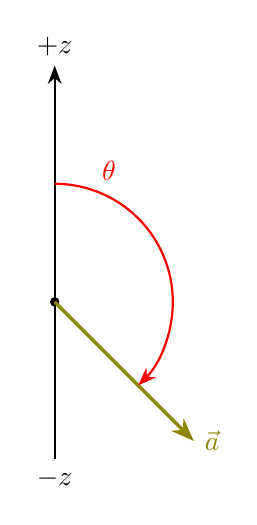
\begin{tikzpicture}[scale=1.0, >=Stealth]
		
		% Draw the vertical z-axis
		\draw[->, thick] (0,-2) -- (0,3) node[above] {$+z$};
		\node[below] at (0,-2) {$-z$};
		
		% Mark the origin point
		\filldraw (0,0) circle (1.5pt);
		
		% Draw the measurement basis vector
		\draw[->, very thick, olive] (0,0) -- (-45:2.5) node[right] {$\vec{a}$};
		
		% Draw the arc representing the angle phi
		\draw[->, red, thick] (0,1.5) arc (90:-45:1.5);
		
		% Add the label for the angle
		\node[red] at (67.5:1.8) {$\theta$};
		
	\end{tikzpicture}
	\caption{Rappresentazione geometrica dell'angolo $\phi$ per la base di misura.}
	\label{fig:measurement_basis}
\end{figure}

Using this basis we obtain the following general form of the Kraus Operators that reads: 
\begin{align}
	\mathcal{K}_{0, \chi_{+}^{a}} &= \cos \left(\frac{\theta}{2}\right) \Big[ \ket{0}\bra{0} + \ket{1}\bra{1} + \cos \left( c \Delta t \right) \ket{2}\bra{2} \Big] - i \sin \left( \frac{\theta}{2} \right) \sin \left( c \Delta t \right) \ket{1}\bra{2} \notag \\ 
	&= \cos \left(\frac{\theta}{2}\right) \mathcal{K}_{0,0} + \sin \left( \frac{\theta}{2} \right) \mathcal{K}_{0,1} \\
	\mathcal{K}_{0, \chi_{-}^{a}} &= \sin \left(\frac{\theta}{2}\right) \Big[ \ket{0}\bra{0} + \ket{1}\bra{1} + \cos \left( c \Delta t \right) \ket{2}\bra{2} \Big] + i \cos \left( \frac{\theta}{2} \right) \sin \left( c \Delta t \right) \ket{1}\bra{2} \notag \\
	&= \sin \left(\frac{\theta}{2}\right) \mathcal{K}_{0,0} - \cos \left( \frac{\theta}{2} \right) \mathcal{K}_{0,1}
\end{align}

These operators respect the completeness rule:
\begin{align}
	\mathcal{K}_{0, \chi_{+}^{a}}^{\dagger} \mathcal{K}_{0, \chi_{+}^{a}} + \mathcal{K}_{0, \chi_{-}^{a}}^{\dagger} \mathcal{K}_{0, \chi_{-}^{a}} &= \left( \cos^2 \left(\frac{\theta}{2}\right) + \sin^2 \left(\frac{\theta}{2}\right) \right) \mathcal{K}_{0,0}^\dagger \mathcal{K}_{0,0} + \left( \sin^2 \left(\frac{\theta}{2}\right) + \cos^2 \left(\frac{\theta}{2}\right) \right) \mathcal{K}_{0,1}^\dagger \mathcal{K}_{0,1} \notag \\
	&= \mathcal{K}_{0,0}^\dagger \mathcal{K}_{0,0} + \mathcal{K}_{0,1}^\dagger \mathcal{K}_{0,1} = \mathbb{I}
\end{align}

We can recover the two limits with these particular angles: 
\begin{itemize}
	\item \textbf{QJ} : $ \theta = 0 \, \rightarrow \,  \mathcal{K}_{0, \chi_{+}^{a}} = \mathcal{K}_{0,0} \, ; \, \mathcal{K}_{0, \chi_{-}^{a}} = \mathcal{K}_{0,1} $
	\item \textbf{SD} : $ \theta = \nicefrac{\pi}{2} \, \rightarrow \,  \mathcal{K}_{0, \chi_{+}^{a}} = \frac{1}{\sqrt{2}} \left( \mathcal{K}_{0,0} + \mathcal{K}_{0,1} \right) \, ; \, \mathcal{K}_{0, \chi_{-}^{a}} = -\frac{1}{\sqrt{2}} \left( \mathcal{K}_{0,0} - \mathcal{K}_{0,1} \right) $
	\item \textit{Alternative QJ Case :} $ \theta = \pi \, \rightarrow \,  \mathcal{K}_{0, \chi_{+}^{a}} = \mathcal{K}_{0,1} \, ; \, \mathcal{K}_{0, \chi_{-}^{a}} = -\mathcal{K}_{0,0} $
\end{itemize}
\subsubsection{General Measurement Probability}
\label{subsub:General_Probability}

To calculate the probability of measuring the Ancilla in the generalized basis states $ \ket{\chi_{+}^{a}} $ or $ \ket{\chi_{-}^{a}} $, we evaluate the expectation value of the corresponding Kraus operators over the system state $ \ket{\Psi_{S}} = \sqrt{p_{0}} \ket{0} + \sqrt{p_{2}} \ket{2} $.

Notice that the cross terms $ \mathcal{K}_{0,0}^\dagger \mathcal{K}_{0,1} $ and $ \mathcal{K}_{0,1}^\dagger \mathcal{K}_{0,0} $ do not contribute to the final probability. These terms map $ \ket{2} $ to $ \ket{1} $ (and vice versa), and since the initial state has no population in $ \ket{1} $, their expectation value is exactly zero:
\begin{equation}
	\bra{\Psi_{S}} \mathcal{K}_{0,0}^\dagger \mathcal{K}_{0,1} \ket{\Psi_{S}} = \bra{\Psi_{S}} \mathcal{K}_{0,1}^\dagger \mathcal{K}_{0,0} \ket{\Psi_{S}} = 0
\end{equation}

To calculate the probability of measuring the Ancilla in the generalized basis states $ \ket{\chi_{+}^{a}} $ or $ \ket{\chi_{-}^{a}} $, we evaluate the expectation value of the corresponding Kraus operators over the general system state $ \ket{\Psi_{S}} = c_{0} \ket{0} + c_{1} \ket{1} + c_{2} \ket{2} $.

Unlike the specific initial state at $ t=0 $, during the dynamical evolution the state $ \ket{1} $ can acquire population ($ p_1 \neq 0 $). Therefore, the cross terms $ \mathcal{K}_{0,0}^\dagger \mathcal{K}_{0,1} $ and $ \mathcal{K}_{0,1}^\dagger \mathcal{K}_{0,0} $ do not vanish, and their sum yields a quantum interference term:
\begin{align}
	\bra{\Psi_{S}} \left( \mathcal{K}_{0,0}^\dagger \mathcal{K}_{0,1} + \mathcal{K}_{0,1}^\dagger \mathcal{K}_{0,0} \right) \ket{\Psi_{S}} &= -i \sin \left( c \Delta t \right) c_{1}^* c_{2} + i \sin \left( c \Delta t \right) c_{2}^* c_{1} \notag \\
	&= 2 \sin \left( c \Delta t \right) \text{Im}(c_1^* c_2)
\end{align}

Using the identity $ 2 \cos\left(\frac{\theta}{2}\right)\sin\left(\frac{\theta}{2}\right) = \sin(\theta) $, the general probabilities become:

\begin{align}
	P_{\chi_{+}^{a}} &= \bra{\Psi_{S}} \mathcal{K}_{0, \chi_{+}^{a}}^{\dagger} \mathcal{K}_{0, \chi_{+}^{a}} \ket{\Psi_{S}} \notag \\
	&= \cos^2 \left(\frac{\theta}{2}\right) \bra{\Psi_{S}} \mathcal{K}_{0,0}^\dagger \mathcal{K}_{0,0} \ket{\Psi_{S}} + \sin^2 \left(\frac{\theta}{2}\right) \bra{\Psi_{S}} \mathcal{K}_{0,1}^\dagger \mathcal{K}_{0,1} \ket{\Psi_{S}} \notag \\
	&\quad + \cos \left(\frac{\theta}{2}\right)\sin \left(\frac{\theta}{2}\right) \bra{\Psi_{S}} \left( \mathcal{K}_{0,0}^\dagger \mathcal{K}_{0,1} + \mathcal{K}_{0,1}^\dagger \mathcal{K}_{0,0} \right) \ket{\Psi_{S}} \notag \\
	&= \cos^2 \left(\frac{\theta}{2}\right) \Big[ p_{0} + p_{1} + p_{2} \cos^2 \left( c \Delta t \right) \Big] + \sin^2 \left(\frac{\theta}{2}\right) \Big[ p_{2} \sin^2 \left( c \Delta t \right) \Big] + \sin(\theta)\sin \left( c \Delta t \right) \text{Im}(c_1^* c_2)
\end{align}

\begin{align}
	P_{\chi_{-}^{a}} &= \bra{\Psi_{S}} \mathcal{K}_{0, \chi_{-}^{a}}^{\dagger} \mathcal{K}_{0, \chi_{-}^{a}} \ket{\Psi_{S}} \notag \\
	&= \sin^2 \left(\frac{\theta}{2}\right) \bra{\Psi_{S}} \mathcal{K}_{0,0}^\dagger \mathcal{K}_{0,0} \ket{\Psi_{S}} + \cos^2 \left(\frac{\theta}{2}\right) \bra{\Psi_{S}} \mathcal{K}_{0,1}^\dagger \mathcal{K}_{0,1} \ket{\Psi_{S}} \notag \\
	&\quad - \cos \left(\frac{\theta}{2}\right)\sin \left(\frac{\theta}{2}\right) \bra{\Psi_{S}} \left( \mathcal{K}_{0,0}^\dagger \mathcal{K}_{0,1} + \mathcal{K}_{0,1}^\dagger \mathcal{K}_{0,0} \right) \ket{\Psi_{S}} \notag \\
	&= \sin^2 \left(\frac{\theta}{2}\right) \Big[ p_{0} + p_{1} + p_{2} \cos^2 \left( c \Delta t \right) \Big] + \cos^2 \left(\frac{\theta}{2}\right) \Big[ p_{2} \sin^2 \left( c \Delta t \right) \Big] - \sin(\theta)\sin \left( c \Delta t \right) \text{Im}(c_1^* c_2)
\end{align}

As a consistency check, it is trivial to verify that evaluating $ P_{\chi_{+}^{a}} + P_{\chi_{-}^{a}} $ perfectly cancels the interference terms and yields $ p_0 + p_1 + p_2 = 1 $.

\newpage 

\subsection{Connection to the SSE formalism}
\label{sub:connection_to_SSE_Photoemission}

As already done in the previous sections, we will analyze the continuous limit of the wavefunction update defined as: 
\begin{equation}
	d\ket{\psi_{S}(t)} = \ket{\psi_{S}(t + \Delta t)} - \ket{\psi_{S}(t)}
\end{equation}
where the state immediately after the collisional step is given by the stochastic unraveling:
\begin{equation}
	\ket{\psi_{S}(t + \Delta t)} = \frac{\mathcal{M}_{0, \chi_{+}^{a}}}{\sqrt{P_{\chi_{+}^{a}}}} \ket{\psi_{S}(t)} (1 - dn) + \frac{\mathcal{M}_{0, \chi_{-}^{a}}}{\sqrt{P_{\chi_{-}^{a}}}} \ket{\psi_{S}(t)} dn
	\label{eq:new_stochastic_update}
\end{equation}
Here, the binary random variable $dn$ follows a Bernoulli distribution, being equal to $1$ with probability $P_{\chi_{-}^{a}}$ and $0$ with probability $P_{\chi_{+}^{a}}$.

The Kraus operators defining the measurement branches are:
\begin{align}
	\mathcal{M}_{0, \chi_{+}^{a}} &= \cos\left(\frac{\theta}{2}\right) \Big[ \ket{0}\bra{0} + \ket{1}\bra{1} + \cos(c \Delta t) \ket{2}\bra{2} \Big] - i \sin\left(\frac{\theta}{2}\right) \sin(c \Delta t) \ket{1}\bra{2} \label{eq:M0_chi_plus} \\
	\mathcal{M}_{0, \chi_{-}^{a}} &= \sin\left(\frac{\theta}{2}\right) \Big[ \ket{0}\bra{0} + \ket{1}\bra{1} + \cos(c \Delta t) \ket{2}\bra{2} \Big] + i \cos\left(\frac{\theta}{2}\right) \sin(c \Delta t) \ket{1}\bra{2} \label{eq:M0_chi_minus}
\end{align}

To ensure complete algebraic consistency, we derive the occurrence probabilities directly from the definition $P_k = \bra{\psi_S(t)} \mathcal{M}_k^\dagger \mathcal{M}_k \ket{\psi_S(t)}$. By expressing the system state in terms of its complex probability amplitudes $c_n = \braket{n|\psi_S(t)}$, such that the corresponding populations are $p_n = |c_n|^2$, and properly accounting for the off-diagonal coherence term between states $\ket{1}$ and $\ket{2}$, the explicit expressions are:
\begin{align}
	P_{\chi_{+}^{a}} &= \cos^2 \left(\frac{\theta}{2}\right) \Big[ p_{0} + p_{1} + p_{2} \cos^2 \left( c \Delta t \right) \Big] + \sin^2 \left(\frac{\theta}{2}\right) \Big[ p_{2} \sin^2 \left( c \Delta t \right) \Big] + \sin(\theta)\sin \left( c \Delta t \right) \text{Im}(c_1^* c_2) \\
	P_{\chi_{-}^{a}} &= \sin^2 \left(\frac{\theta}{2}\right) \Big[ p_{0} + p_{1} + p_{2} \cos^2 \left( c \Delta t \right) \Big] + \cos^2 \left(\frac{\theta}{2}\right) \Big[ p_{2} \sin^2 \left( c \Delta t \right) \Big] - \sin(\theta)\sin \left( c \Delta t \right) \text{Im}(c_1^* c_2)
\end{align}

Substituting the explicit Kraus operators of Eqs.~\eqref{eq:M0_chi_plus}-\eqref{eq:M0_chi_minus} 
and the associated probabilities into Eq.~\eqref{eq:new_stochastic_update}, we obtain the 
fully explicit stochastic update:
{\footnotesize
\begin{align}
	&\ket{\psi_{S}\left(t + \Delta t \right)} = \notag \\
	&= \frac{\cos\left(\dfrac{\theta}{2}\right) \Big[ \ket{0}\bra{0} + \ket{1}\bra{1} + \cos\left(c\Delta t\right)\ket{2}\bra{2} \Big] 
	- i\sin\left(\dfrac{\theta}{2}\right)\sin\left(c\Delta t\right)\ket{1}\bra{2}} {\sqrt{\cos^{2}\left(\dfrac{\theta}{2}\right)\Big[p_{0}+p_{1}+p_{2}\cos^{2}(c\Delta t)\Big] + \sin^{2}\left(\dfrac{\theta}{2}\right)\Big[p_{2}\sin^{2}(c\Delta t)\Big] + \sin(\theta)\sin(c\Delta t) \text{Im}(c_{1}^{*}c_{2})}} \ket{\psi_{S}\left(t\right)} \left(1-dn\right) \notag \\[14pt]
	&\quad + \frac{\sin\left(\dfrac{\theta}{2}\right) \Big[ \ket{0}\bra{0} + \ket{1}\bra{1} + \cos\left(c\Delta t\right)\ket{2}\bra{2} \Big] + i\cos\left(\dfrac{\theta}{2}\right)\sin\left(c\Delta t\right)\ket{1}\bra{2}} {\sqrt{\sin^{2}\left(\dfrac{\theta}{2}\right)\Big[p_{0}+p_{1}+p_{2}\cos^{2}(c\Delta t)\Big] + \cos^{2}\left(\dfrac{\theta}{2}\right)\Big[p_{2}\sin^{2}(c\Delta t)\Big] - \sin(\theta)\sin(c\Delta t) \text{Im}(c_{1}^{*}c_{2})}} \ket{\psi_{S}\left(t\right)} dn \label{eq:full_substitution_photoemission}
\end{align}
}

Setting $c = \sqrt{\Gamma/\Delta t}$, we have $c\Delta t = \sqrt{\Gamma\Delta t} \to 0$ 
as $\Delta t \to 0$. Expanding the trigonometric functions of $c\Delta t$ to leading 
order in $\Delta t$:
\begin{align}
	\cos(c\Delta t) &\approx 1 - \frac{(c\Delta t)^{2}}{2} = 1 - \frac{\Gamma\Delta t}{2}, 
	\label{eq:cos_cdt_expansion} \\
	\sin(c\Delta t) &\approx c\Delta t = \sqrt{\Gamma\Delta t}, 
	\label{eq:sin_cdt_expansion} \\
	\cos^{2}(c\Delta t) &\approx 1 - \Gamma\Delta t, 
	\label{eq:cos2_cdt_expansion} \\
	\sin^{2}(c\Delta t) &\approx \Gamma\Delta t. 
	\label{eq:sin2_cdt_expansion}
\end{align}

Substituting Eqs.\ref{eq:cos_cdt_expansion} and \ref{eq:sin_cdt_expansion} into 
$\mathcal{M}_{0,\chi_{+}^{a}}$ and $\mathcal{M}_{0,\chi_{-}^{a}}$:
\begin{align}
	\mathcal{M}_{0, \chi_{+}^{a}} &\approx \cos\left(\frac{\theta}{2}\right) 
	\Big[ \ket{0}\bra{0} + \ket{1}\bra{1} + \left(1-\frac{\Gamma\Delta t}{2}\right)\ket{2}\bra{2} \Big] 
	- i \sin\left(\frac{\theta}{2}\right) \sqrt{\Gamma\Delta t}\; \ket{1}\bra{2} \notag \\
	&= \cos\left(\frac{\theta}{2}\right) \left[ \mathbb{I} - \frac{\Gamma\Delta t}{2}\ket{2}\bra{2} \right] 
	- i \sin\left(\frac{\theta}{2}\right) \sqrt{\Gamma\Delta t}\; \ket{1}\bra{2}, 
	\label{eq:M0_chiplus_expanded} \\[8pt]
	\mathcal{M}_{0, \chi_{-}^{a}} &\approx \sin\left(\frac{\theta}{2}\right) 
	\left[ \mathbb{I} - \frac{\Gamma\Delta t}{2}\ket{2}\bra{2} \right] 
	+ i \cos\left(\frac{\theta}{2}\right) \sqrt{\Gamma\Delta t}\; \ket{1}\bra{2}. 
	\label{eq:M0_chiminus_expanded}
\end{align}

Similarly, substituting Eqs.\ref{eq:cos2_cdt_expansion} and \ref{eq:sin2_cdt_expansion} 
into $P_{\chi_{+}^{a}}$, and using the normalization $p_{0}+p_{1}+p_{2}=1$:
\begin{align}
	P_{\chi_{+}^{a}} &\approx \cos^{2}\left(\frac{\theta}{2}\right) 
	\Big[ p_{0}+p_{1}+p_{2}\left(1-\Gamma\Delta t\right) \Big] 
	+ \sin^{2}\left(\frac{\theta}{2}\right) p_{2}\,\Gamma\Delta t 
	+ \sin(\theta)\sqrt{\Gamma\Delta t}\;\text{Im}(c_{1}^{*}c_{2}) \notag \\
	&= \cos^{2}\left(\frac{\theta}{2}\right) 
	- \Gamma\Delta t\, p_{2}\Big[\cos^{2}\left(\frac{\theta}{2}\right)-\sin^{2}\left(\frac{\theta}{2}\right)\Big] 
	+ \sin(\theta)\sqrt{\Gamma\Delta t}\;\text{Im}(c_{1}^{*}c_{2}) \notag \\
	&= \cos^{2}\left(\frac{\theta}{2}\right) - \Gamma\Delta t\, p_{2}\cos\theta 
	+ \sin(\theta)\sqrt{\Gamma\Delta t}\;\text{Im}(c_{1}^{*}c_{2}), 
	\label{eq:P_chiplus_expanded}
\end{align}
where we used $\cos^{2}(\theta/2)-\sin^{2}(\theta/2)=\cos\theta$. Analogously:
\begin{equation}
	P_{\chi_{-}^{a}} \approx \sin^{2}\left(\frac{\theta}{2}\right) + \Gamma\Delta t\, p_{2}\cos\theta 
	- \sin(\theta)\sqrt{\Gamma\Delta t}\;\text{Im}(c_{1}^{*}c_{2}).
	\label{eq:P_chiminus_expanded}
\end{equation}
As a consistency check, $P_{\chi_{+}^{a}}+P_{\chi_{-}^{a}} = \cos^{2}(\theta/2)+\sin^{2}(\theta/2) = 1$ 
exactly, with both the $O(\Delta t)$ and $O(\sqrt{\Delta t})$ correction terms cancelling between the two branches.

For brevity we use $c_{\theta}\equiv\cos(\theta/2)$, $s_{\theta}\equiv\sin(\theta/2)$, and $I \equiv \text{Im}(c_{1}^{*}c_{2})$.

Writing $P_{\chi_{+}^{a}} = c_{\theta}^{2}\left[1+\varepsilon_{+}\right]$ with 
$\varepsilon_{+} = -\dfrac{\Gamma\Delta t\, p_{2}\cos\theta}{c_{\theta}^{2}} 
+ \dfrac{\sin\theta\sqrt{\Gamma\Delta t}\,I}{c_{\theta}^{2}}$, and expanding 
$(1+\varepsilon_{+})^{-1/2} \approx 1-\varepsilon_{+}/2+\frac{3}{8}\varepsilon_{+}^{2}$ 
(retaining the $O(\Delta t)$ contribution generated by the square of the 
$O(\sqrt{\Delta t})$ term), we obtain:
\begin{align}
	\frac{1}{\sqrt{P_{\chi_{+}^{a}}}} &\approx \frac{1}{c_{\theta}} 
	\left[ 1 + \frac{\Gamma\Delta t\, p_{2}\cos\theta}{2c_{\theta}^{2}} 
	- \frac{\sin\theta\, I}{2c_{\theta}^{2}}\sqrt{\Gamma\Delta t} 
	+ \frac{3\sin^{2}\theta\, I^{2}}{8c_{\theta}^{4}}\,\Gamma\Delta t \right]
	\label{eq:expansion_Pchiplus} \\
	\frac{1}{\sqrt{P_{\chi_{-}^{a}}}} &\approx \frac{1}{s_{\theta}} 
	\left[ 1 - \frac{\Gamma\Delta t\, p_{2}\cos\theta}{2s_{\theta}^{2}} 
	+ \frac{\sin\theta\, I}{2s_{\theta}^{2}}\sqrt{\Gamma\Delta t} 
	+ \frac{3\sin^{2}\theta\, I^{2}}{8s_{\theta}^{4}}\,\Gamma\Delta t \right]
	\label{eq:expansion_Pchiminus}
\end{align}
Note the new feature compared to the exciton dimer case: the $I^{2}$ term is a genuinely nonlinear (state-dependent) correction to the normalization, structurally analogous to the nonlinear terms appearing in the standard nonlinear QSD formalism 
(cf.\ Eq.\ref{eq:standard_SD_SSE}).

Substituting the expansions of $\mathcal{M}_{0,\chi_{+}^{a}}$ 
(Eq.\ref{eq:M0_chiplus_expanded}) and $1/\sqrt{P_{\chi_{+}^{a}}}$ 
(Eq.\ref{eq:expansion_Pchiplus}), and retaining all terms up to $O(\Delta t)$ 
(including the $O(\sqrt{\Delta t})\times O(\sqrt{\Delta t})$ cross term between the 
$\ket{1}\bra{2}$ piece of $\mathcal{M}_{0,\chi_{+}^{a}}$ and the $I$-term of 
$1/\sqrt{P_{\chi_{+}^{a}}}$), we obtain:
\begin{align}
	\frac{\mathcal{M}_{0,\chi_{+}^{a}}}{\sqrt{P_{\chi_{+}^{a}}}} &\approx 
	\mathbb{I} - \frac{\sin\theta\, I}{2c_{\theta}^{2}}\sqrt{\Gamma\Delta t}\,\mathbb{I} 
	- i\,\frac{s_{\theta}}{c_{\theta}}\sqrt{\Gamma\Delta t}\,\ket{1}\bra{2} \notag \\
	&\quad + \Gamma\Delta t \left[ \frac{p_{2}\cos\theta}{2c_{\theta}^{2}}\mathbb{I} 
	+ \frac{3\sin^{2}\theta\, I^{2}}{8c_{\theta}^{4}}\mathbb{I} 
	- \frac{1}{2}\ket{2}\bra{2} 
	+ i\,\frac{s_{\theta}\sin\theta\, I}{2c_{\theta}^{3}}\ket{1}\bra{2} \right]
	\label{eq:norm_Mchiplus}
\end{align}
and analogously:
\begin{align}
	\frac{\mathcal{M}_{0,\chi_{-}^{a}}}{\sqrt{P_{\chi_{-}^{a}}}} &\approx 
	+\mathbb{I} + \frac{\sin\theta\, I}{2s_{\theta}^{2}}\sqrt{\Gamma\Delta t}\,\mathbb{I} 
	+ i\,\frac{c_{\theta}}{s_{\theta}}\sqrt{\Gamma\Delta t}\,\ket{1}\bra{2} \notag \\
	&\quad + \Gamma\Delta t \left[ -  \frac{p_{2}\cos\theta}{2s_{\theta}^{2}}\mathbb{I} 
	+ \frac{3\sin^{2}\theta\, I^{2}}{8s_{\theta}^{4}}\mathbb{I} 
	- \frac{1}{2}\ket{2}\bra{2} 
	+ i\,\frac{c_{\theta}\sin\theta\, I}{2s_{\theta}^{3}}\ket{1}\bra{2} \right]
	\label{eq:norm_Mchiminus}
\end{align}

Substituting Eqs.\ref{eq:norm_Mchiplus} and \ref{eq:norm_Mchiminus} into the 
generic state update equation, the wavefunction at $t+\Delta t$ reads:
\begin{align}
	\ket{\psi_{S}\left(t+\Delta t\right)} &= 
	\Bigg\{ \mathbb{I} - \frac{\sin\theta\, I}{2c_{\theta}^{2}}\sqrt{\Gamma\Delta t}\,\mathbb{I} 
	- i\,\frac{s_{\theta}}{c_{\theta}}\sqrt{\Gamma\Delta t}\,\ket{1}\bra{2} \notag \\
	&\hphantom{=\Bigg\{} + \Gamma\Delta t \left[ \left(\frac{p_{2}\cos\theta}{2c_{\theta}^{2}} 
	+ \frac{3\sin^{2}\theta\, I^{2}}{8c_{\theta}^{4}}\right)\mathbb{I} 
	- \frac{1}{2}\ket{2}\bra{2} 
	+ i\,\frac{s_{\theta}\sin\theta\, I}{2c_{\theta}^{3}}\ket{1}\bra{2} \right] \Bigg\} 
	\ket{\psi_{S}(t)} \left(1-dn\right) \notag \\[10pt]
	&\quad + \Bigg\{ \mathbb{I} + \frac{\sin\theta\, I}{2s_{\theta}^{2}}\sqrt{\Gamma\Delta t}\,\mathbb{I} 
	+ i\,\frac{c_{\theta}}{s_{\theta}}\sqrt{\Gamma\Delta t}\,\ket{1}\bra{2} \notag \\
	&\hphantom{=\Bigg\{} + \Gamma\Delta t \left[  \left( -\frac{p_{2}\cos\theta}{2s_{\theta}^{2}} 
	+ \frac{3\sin^{2}\theta\, I^{2}}{8s_{\theta}^{4}}\right)\mathbb{I} 
	- \frac{1}{2}\ket{2}\bra{2} 
	+ i\,\frac{c_{\theta}\sin\theta\, I}{2s_{\theta}^{3}}\ket{1}\bra{2} \right] \Bigg\} 
	\ket{\psi_{S}(t)} \, dn
	\label{eq:psi_t_plus_dt_photoemission_expanded}
\end{align}


\subsection{Continuous Limit: Recovering the State Diffusion Equation}

To recover the standard State Diffusion limit, we set the measurement angle to $ \theta = \pi/2 $. In this regime, the trigonometric coefficients simplify to $ \cos(\theta) = 0 $, $ \sin(\theta) = 1 $, and $ c_\theta = s_\theta = 1/\sqrt{2} $. 

Because $ \cos(\pi/2) = 0 $, the $ \mathcal{O}(\Delta t) $ population term proportional to $ p_2 $ identically vanishes from the probability expansions. Substituting these values into the state update equation (Eq.~\ref{eq:psi_t_plus_dt_photoemission_expanded}) and grouping the deterministic $ \mathcal{O}(\Delta t) $ and stochastic $ \mathcal{O}(\sqrt{\Delta t}) $ terms, the differential change $ d\ket{\psi_S} = \ket{\psi_S(t+\Delta t)} - \ket{\psi_S(t)} $ yields:

\begin{align}
	d\ket{\psi_{S}} &= \left[ \frac{3}{2}\Gamma I^2 \mathbb{I} - \frac{1}{2}\Gamma\ket{2}\bra{2} + i \Gamma I \ket{1}\bra{2} \right] \Delta t \ket{\psi_{S}} \notag \\
	&\quad + \left[ -I\sqrt{\Gamma}\mathbb{I} - i\sqrt{\Gamma}\ket{1}\bra{2} \right] \sqrt{\Delta t} (1 - 2dn) \ket{\psi_{S}}
	\label{eq:raw_SD_update}
\end{align}
where we have used the fact that the deterministic brackets in the two branches (multiplied by $ 1-dn $ and $ dn $) are now identical, while the stochastic brackets carry opposite signs.

To connect this result to standard open quantum systems notation, we define the physical jump operator:
\begin{equation}
	c = i\sqrt{\Gamma}\ket{1}\bra{2} \quad \implies \quad c^\dagger = -i\sqrt{\Gamma}\ket{2}\bra{1}
\end{equation}
The expectation value of its Hermitian part is purely related to the imaginary part of the coherence $ I = \text{Im}(c_1^* c_2) $:
\begin{equation}
	\langle c + c^\dagger \rangle = i\sqrt{\Gamma}(c_1^* c_2 - c_2^* c_1) = -2\sqrt{\Gamma}\text{Im}(c_1^* c_2) = -2\sqrt{\Gamma}I \quad \implies \quad \sqrt{\Gamma}I = -\frac{1}{2}\langle c + c^\dagger \rangle
	\label{eq:expectation_jump}
\end{equation}

In the standard framework of Itô calculus, a Stochastic Schrödinger Equation (SSE) separates the evolution of the system into a deterministic continuous evolution and a stochastic state update conditioned on a noisy measurement record $ d\tilde{Y} $:
\begin{equation}
	d\ket{\psi_{S}} = A_{raw} \ket{\psi_{S}} dt + B \ket{\psi_{S}} d\tilde{Y}
	\label{eq:general_SDE_structure}
\end{equation}
By defining the raw homodyne measurement record as $ d\tilde{Y} = (2dn - 1)\sqrt{\Delta t} $, setting $ dt = \Delta t $, and substituting the definitions of $ c $ and $ \langle c + c^\dagger \rangle $ into Eq.\ref{eq:raw_SD_update}, we can explicitly identify the raw drift operator $ A_{raw} $ and the diffusion operator $ B $:
\begin{align}
	A_{raw} &= \frac{3}{8}\langle c + c^\dagger \rangle^2 \mathbb{I} - \frac{1}{2}c^\dagger c - \frac{1}{2}\langle c + c^\dagger \rangle c \\
	B &= c - \frac{1}{2}\langle c + c^\dagger \rangle
\end{align}

However, $ d\tilde{Y} $ is \emph{not} a standard Wiener increment because its expected value is not zero. Using the probability of the jump branch $ P_{\chi_{-}^{a}} \approx \frac{1}{2} - \sqrt{\Gamma \Delta t}I $, the expectation value evaluates to:
\begin{equation}
	\mathbb{E}[d\tilde{Y}] = \left(2 P_{\chi_{-}^{a}} - 1\right)\sqrt{\Delta t} = -2\sqrt{\Gamma \Delta t}I \sqrt{\Delta t} = \langle c + c^\dagger \rangle dt
\end{equation}

To cast the equation into a proper Itô Stochastic Differential Equation, we must define a centered, zero-mean Wiener increment $ dW $:
\begin{equation}
	dW = d\tilde{Y} - \mathbb{E}[d\tilde{Y}] = d\tilde{Y} - \langle c + c^\dagger \rangle dt \quad \implies \quad d\tilde{Y} = dW + \langle c + c^\dagger \rangle dt
\end{equation}
Substituting this back into the evolution generates an Itô drift correction. The final effective drift operator $ A_{eff} $ reads:
\begin{align}
	A_{eff} &= A_{raw} + B \langle c + c^\dagger \rangle \notag \\
	&= \left( -\frac{1}{2}c^\dagger c - \frac{1}{2}\langle c + c^\dagger \rangle c + \frac{3}{8}\langle c + c^\dagger \rangle^2 \right) + \left( c - \frac{1}{2}\langle c + c^\dagger \rangle \right) \langle c + c^\dagger \rangle \notag \\
	&= -\frac{1}{2}c^\dagger c + \frac{1}{2}\langle c + c^\dagger \rangle c - \frac{1}{8}\langle c + c^\dagger \rangle^2 \notag \\
	&= -\frac{1}{2}\left( c^\dagger c - \langle c + c^\dagger \rangle c + \frac{1}{4}\langle c + c^\dagger \rangle^2 \right)
\end{align}

Replacing $ A_{eff} $ and the true Wiener increment $ dW $ into the differential update, we exactly recover the standard nonlinear State Diffusion (Homodyne) equation:
\begin{equation}
	d\ket{\psi_{S}} = \left[ -\frac{1}{2}\left(c^\dagger c - \langle c + c^\dagger \rangle c + \frac{1}{4}\langle c + c^\dagger \rangle^2 \right)dt + \left(c - \frac{\langle c + c^\dagger \rangle}{2}\right)dW \right] \ket{\psi_{S}}
\end{equation}

\subsection{Continuous Limit: Recovering the Quantum Jump Equation}

If we directly substitute $ \theta = 0 $ into the generalized expanded equation, some terms appear to diverge. This occurs because the Taylor expansion of $ 1/\sqrt{P_{\chi_{-}^{a}}} $ performed earlier implicitly assumed $ \sin(\theta/2) \neq 0 $ as its leading-order constant. To correctly recover the Quantum Jump (QJ) limit, we must set $ \theta = 0 $ \emph{before} expanding the normalizations.

Setting $ \theta = 0 $, the measurement basis aligns with the computational basis, and the modified Kraus operators reduce directly to the standard QJ branches:
\begin{align}
	\mathcal{M}_{0, \chi_{+}^{a}} &= \mathcal{K}_{0,0} \approx \mathbb{I} - \frac{1}{2} c^\dagger c \Delta t \\
	\mathcal{M}_{0, \chi_{-}^{a}} &= -\mathcal{K}_{0,1} \approx c \sqrt{\Delta t}
\end{align}
where we defined the jump operator $ c = i\sqrt{\Gamma}\ket{1}\bra{2} $, meaning $ c^\dagger c = \Gamma\ket{2}\bra{2} $. The corresponding expectation value yields the correct population term $ \langle c^\dagger c \rangle = p_2 \Gamma $.

The occurrence probabilities evaluate exactly to:
\begin{align}
	P_{\chi_{+}^{a}} &= 1 - \langle c^\dagger c \rangle \Delta t \\
	P_{\chi_{-}^{a}} &= \langle c^\dagger c \rangle \Delta t
\end{align}

We can now evaluate the state update for the two distinct branches independently.
For the no-jump branch ($ dn = 0 $), we expand the denominator up to $ \mathcal{O}(\Delta t) $:
\begin{align}
	\frac{\mathcal{M}_{0, \chi_{+}^{a}}}{\sqrt{P_{\chi_{+}^{a}}}} \ket{\psi_{S}} &\approx \left( \mathbb{I} - \frac{1}{2} c^\dagger c \Delta t \right) \left( 1 + \frac{1}{2} \langle c^\dagger c \rangle \Delta t \right) \ket{\psi_{S}} \notag \\
	&\approx \left[ \mathbb{I} - \frac{1}{2} \left( c^\dagger c - \langle c^\dagger c \rangle \right) \Delta t \right] \ket{\psi_{S}}
\end{align}

For the jump branch ($ dn = 1 $), the $ \sqrt{\Delta t} $ factors in the numerator and denominator perfectly cancel out, avoiding any divergence:
\begin{equation}
	\frac{\mathcal{M}_{0, \chi_{-}^{a}}}{\sqrt{P_{\chi_{-}^{a}}}} \ket{\psi_{S}} = \frac{c \sqrt{\Delta t}}{\sqrt{\langle c^\dagger c \rangle \Delta t}} \ket{\psi_{S}} = \frac{c}{\sqrt{\langle c^\dagger c \rangle}} \ket{\psi_{S}}
\end{equation}

Substituting these branches back into the differential update $ d\ket{\psi_{S}} = \ket{\psi_{S}(t+\Delta t)} - \ket{\psi_{S}(t)} $, and setting $ \Delta t \to dt $, we obtain:
\begin{equation}
	d\ket{\psi_{S}} = \left[ \left( \mathbb{I} - \frac{1}{2} \left( c^\dagger c - \langle c^\dagger c \rangle \right) dt \right) (1 - dn) + \frac{c}{\sqrt{\langle c^\dagger c \rangle}} dn - \mathbb{I} \right] \ket{\psi_{S}}
\end{equation}

In the Itô calculus for point processes, $ dn $ represents a macroscopic jump event ($ dn^2 = dn $), but its occurrence probability is $ \mathcal{O}(dt) $. Therefore, cross terms like $ dn \cdot dt $ scale as $ \mathcal{O}(dt^2) $ and vanish. Expanding the brackets and grouping the remaining terms, we perfectly recover the standard Quantum Jump SSE:
\begin{equation}
	d\ket{\psi_{S}} = \left[ -\frac{1}{2}\left(c^\dagger c - \langle c^\dagger c \rangle\right)dt + \left( \frac{c}{\sqrt{\langle c^\dagger c \rangle}} - \mathbb{I} \right)dn \right] \ket{\psi_{S}}
	\label{eq:standard_QJ_SSE}
\end{equation}

\paragraph{Universal Wiener limit for $\theta \neq 0,\pi$.}
We now show that the generalized stochastic update for the 3-level photoemission model converges to the \emph{same} diffusive State Diffusion equation for any fixed $\theta \in (0,\pi)$. 

Let us isolate the stochastic $ \mathcal{O}(\sqrt{\Delta t}) $ fluctuations in the state update (Eq.~\ref{eq:psi_t_plus_dt_photoemission_expanded}). Denoting the $ \mathcal{O}(\sqrt{\Delta t}) $ brackets for the jump ($dn=1$) and no-jump ($dn=0$) branches as $ \mathcal{F}_{-} $ and $ \mathcal{F}_{+} $ respectively, the total stochastic term reads:
\begin{equation}
	\mathcal{F}_{stoch} = \mathcal{F}_{+} (1 - dn) + \mathcal{F}_{-} dn = \mathcal{F}_{+} + (\mathcal{F}_{-} - \mathcal{F}_{+}) dn
\end{equation}

By expanding $ dn = \mathbb{E}[dn] + \delta n \approx \sin^2(\theta/2) + \delta n $, the fluctuation is entirely driven by the zero-mean random variable $ \delta n $. The coefficient multiplying this fluctuation is the difference between the two branches:
\begin{align}
	\mathcal{F}_{-} - \mathcal{F}_{+} &= \left[ \frac{\sin\theta\, I}{2 s_{\theta}^{2}} \mathbb{I} + i\,\frac{c_{\theta}}{s_{\theta}} \ket{1}\bra{2} \right] \sqrt{\Gamma\Delta t} - \left[ -\frac{\sin\theta\, I}{2 c_{\theta}^{2}} \mathbb{I} - i\,\frac{s_{\theta}}{c_{\theta}} \ket{1}\bra{2} \right] \sqrt{\Gamma\Delta t} \notag \\
	&= \left[ \frac{\sin\theta\, I}{2} \left( \frac{1}{s_{\theta}^{2}} + \frac{1}{c_{\theta}^{2}} \right) \mathbb{I} + i \left( \frac{c_{\theta}}{s_{\theta}} + \frac{s_{\theta}}{c_{\theta}} \right) \ket{1}\bra{2} \right] \sqrt{\Gamma\Delta t}
\end{align}
Using the trigonometric identities $ \frac{1}{s_{\theta}^{2}} + \frac{1}{c_{\theta}^{2}} = \frac{s_{\theta}^{2} + c_{\theta}^{2}}{s_{\theta}^{2} c_{\theta}^{2}} = \frac{4}{\sin^2\theta} $ and $ \frac{c_{\theta}}{s_{\theta}} + \frac{s_{\theta}}{c_{\theta}} = \frac{2}{\sin\theta} $, the difference dramatically simplifies to:
\begin{equation}
	\mathcal{F}_{-} - \mathcal{F}_{+} = \frac{2}{\sin\theta} \left[ I \sqrt{\Gamma} \mathbb{I} + i\sqrt{\Gamma} \ket{1}\bra{2} \right] \sqrt{\Delta t}
\end{equation}

Multiplying this by the fluctuation $ \delta n $ yields the pure noise term:
\begin{equation}
	(\mathcal{F}_{-} - \mathcal{F}_{+}) \delta n = \left[ I \sqrt{\Gamma} \mathbb{I} + i\sqrt{\Gamma} \ket{1}\bra{2} \right] \left( \frac{2}{\sin\theta} \delta n \sqrt{\Delta t} \right)
\end{equation}

We recognize the second parenthesis as the universally rescaled Wiener increment defined previously:
\begin{equation}
	\Delta W \equiv \frac{2}{\sin(\theta)}\,\delta n\,\sqrt{\Delta t}
\end{equation}
which satisfies $ \mathbb{E}[\Delta W] = 0 $ and $ \mathbb{E}[\Delta W^2] = \Delta t $. 

Furthermore, substituting the physical operator definitions $ c = i\sqrt{\Gamma}\ket{1}\bra{2} $ and $ I\sqrt{\Gamma} = -\frac{1}{2}\langle c + c^\dagger \rangle $, the structural bracket perfectly reconstructs the diffusion operator $ B $:
\begin{equation}
	I \sqrt{\Gamma} \mathbb{I} + i\sqrt{\Gamma} \ket{1}\bra{2} = -\frac{1}{2}\langle c + c^\dagger \rangle \mathbb{I} + c = B
\end{equation}

Thus, the stochastic contribution for \emph{any} arbitrary angle $ \theta \in (0, \pi) $ is identically $ B \Delta W $. By performing the same algebraic grouping for the deterministic $ \mathcal{O}(\Delta t) $ drift terms (where all $ \theta $ dependencies rigorously cancel out against the zeroth-order terms of $ \mathbb{E}[dn] $), the full state update collapses exactly into the universal nonlinear State Diffusion equation:
\begin{equation}
	d\ket{\psi_{S}} = A_{eff} dt + B dW
\end{equation}

\paragraph{Singular limits: $\theta=0$ and $\theta=\pi$.}
As established in the previous models, this universality strictly requires $ \sin\theta \neq 0 $. At the boundary points $ \theta = 0 $ and $ \theta = \pi $, the variance scaling breaks down because the probability of one branch scales as $ \mathcal{O}(\Delta t) $ rather than $ \mathcal{O}(1) $. At these isolated singularities, the noise converges to a compound Poisson process rather than a continuous Wiener process, gracefully recovering the Quantum Jump unravellings derived in Eq.~\ref{eq:standard_QJ_SSE}.

\newpage 

\subsection{Some Results}
\label{sub:coccia3levels_results}
In this subsection we show some of the results of this specific case study.

\subsubsection{Finite-Sample Convergence Analysis}
\label{subsub:finite_sample_convergence_analysis}

By comparing the numerical averages over $N = 10000$ trajectories with the exact Lindblad dynamics (and the map obtained by tracing out the ancilla's degrees of freedom), we observe distinct convergence behaviors for the two unravelings. Specifically, the State Diffusion (SD) unraveling successfully reaches convergence for all three population observables. In contrast, the Quantum Jump (QJ) unraveling struggles to converge for the populations of states $\ket{0}$ and $\ket{1}$ when the ensemble size is insufficiently large.

To quantify this discrepancy, we analyzed the convergence error—measured via Trace Distance—as a function of the number of averaged trajectories $N$. This analysis reveals that the two limits are governed by fundamentally different statistical regimes: the SD limit is ruled by the \textbf{Central Limit Theorem} (CLT), whereas the QJ limit is governed by the \textbf{Law of Rare Events}, also known as the \textbf{Poisson Limit Theorem}.

In the SD limit, the system's evolution is continuously driven by a Wiener process, which is characterized by normally distributed increments. Because the underlying noise is Gaussian at every time step, the statistical fluctuations of the ensemble average follow the CLT from the very beginning. Consequently, the convergence error scales symmetrically and smoothly as $1/\sqrt{N}$, even for a relatively low number of trajectories.

Conversely, the QJ dynamics consist of long periods of deterministic, non-unitary evolution interrupted by abrupt, highly improbable quantum jumps. Let $p$ be the overall probability that a given trajectory undergoes at least one jump during the total simulation time. Since $p \ll 1$, the occurrence of these jumps across an ensemble of $N$ independent trajectories is perfectly described by the Poisson Limit Theorem. This theorem states that as the number of trials $N \to \infty$ and the success probability $p \to 0$, while their product $\lambda = Np$ remains constant, the binomial distribution of the events converges to a Poisson distribution with mean $\lambda$.

The Poissonian nature of the QJ unraveling strictly dictates the minimum number of trajectories required to correctly sample the dissipative dynamics. If $\lambda \ll 1$, the ensemble will most likely not record a single jump, leaving the dissipative channels unpopulated and causing the numerical error to plateau at a maximum constant value. According to the Poisson distribution, the probability of observing exactly $k$ jumping trajectories in the ensemble is :
\begin{equation}
	P(k) = \frac{\lambda^k e^{-\lambda}}{k!}
\end{equation}
Thus, the probability of observing \textit{at least one} jump is:
\begin{equation}
	P(k \ge 1) = 1 - P(0) = 1 - e^{-N p}
\end{equation}

To ensure that the simulation captures the quantum jumps with a defined statistical confidence level, we can analytically determine the critical ensemble size. For instance, to achieve a $95\%$ probability of observing at least one jump, we require:
\begin{align}
	1 - e^{-N p} &= 0.95 \notag \\
	e^{-N p} &= 0.05 \notag \\
	N &= \frac{-\ln(0.05)}{p} \approx \frac{3}{p}
	\label{eq:critical_trajectories}
\end{align}

This result formally explains the initial plateau observed in the Trace Distance scaling for the QJ unraveling: below this critical threshold $N$, the Monte Carlo algorithm fails to sample the rare event, yielding an incomplete representation of the system's density matrix. Only when $N \gg 3/p$ does the Poisson distribution accumulate enough events to eventually transition into a Gaussian regime, restoring the expected $1/\sqrt{N}$ convergence scaling.

\subsubsection{Analysis of the presume null Variance of the Population of Site $ \ket{2} $}
In all the regime, different from QJ, we  see that a single trajectory reproduce exactly the same Lindblad evolution, without need to average over different realizations. We try to evaluate the evolution of the population of site $ \ket{2} $ and see if we have a cancellation of the noisy part.
We start again from the equation : 
\begin{equation}
	\ket{\psi_{S}(t + \Delta t)} = \frac{\mathcal{K}_{0}}{\sqrt{P_{0}}} \ket{\psi_{S}(t)} (1 - dn) + \frac{\mathcal{K}_{1}}{\sqrt{P_{1}}} \ket{\psi_{S}(t)} dn
\end{equation}
and define the population after the collisional time step as : 
\begin{align}
	&p_{2} \left( t + \Delta t \right) = \bra{\psi_{S}(t + \Delta t)} 2 \rangle \langle 2 \ket{\psi_{S}(t + \Delta t)} \notag \\ 
	&= \bra{\psi_{S}(t)} \left( \frac{\mathcal{K}^{\dagger}_{0}}{\sqrt{P_{0}}}  (1 - dn) + \frac{\mathcal{K}^{\dagger}_{1}}{\sqrt{P_{1}} } dn\right) \ket{2} \bra{2} \left( \frac{\mathcal{K}_{0}}{\sqrt{P_{0}}} (1 - dn) + \frac{\mathcal{K}_{1}}{\sqrt{P_{1}}} dn \right) \ket{\psi_{S}(t)} \notag \\
	&= \frac{\bra{\psi_{S}(t)} {K}^{\dagger}_{0} \ket{2} \bra{2} {K}_{0} \ket{\psi_{S}(t)} }{P_{0}} (1-dn) + \frac{\bra{\psi_{S}(t)} {K}^{\dagger}_{1} \ket{2} \bra{2} {K}_{1} \ket{\psi_{S}(t)} }{P_{1}} dn
\end{align}
remembering the properties of the Bernoulli variable $ dn^{2} = dn $ and so $ (1-dn)dn = 0 $.
We can now explicit the product between the Kraus Operators and the projectors : 
\begin{gather}
	{K}^{\dagger}_{0} \ket{2} \bra{2} {K}_{0} = \cos^{2} \left( \frac{\theta}{2} \right) \cos^{2} \left( c \Delta t \right) \ket{2} \bra{2} \\
	{K}^{\dagger}_{1} \ket{2} \bra{2} {K}_{1} = \sin^{2} \left( \frac{\theta}{2} \right) \cos^{2} \left( c \Delta t \right) \ket{2} \bra{2} 
\end{gather}
so that, with $ \bra{\psi_{S}(t)} 2 \rangle \langle 2 \ket{\psi_{S}(t)} = p_{2} (t) $, we got 
\begin{align}
	p_{2} \left( t + \Delta t \right) &= \frac{\cos^{2} \left( \frac{\theta}{2} \right) \cos^{2} \left( c \Delta t \right) p_{2} (t)}{P_{0}} (1-dn) + \frac{\sin^{2} \left( \frac{\theta}{2} \right) \cos^{2} \left( c \Delta t \right) p_{2} (t)}{P_{1}} dn \\
	&=  \cos^{2} \left( c \Delta t \right) p_{2} (t) \Big[ \frac{\cos^{2} \left( \frac{\theta}{2} \right)}{P_{0}} + \left( \frac{\sin^{2} \left( \frac{\theta}{2} \right)}{P_{1}} - \frac{\cos^{2} \left( \frac{\theta}{2} \right)}{P_{0}} \right) dn \Big] \label{eq:general_p2_evolution}
\end{align}
We can now analyze the two unraveling limits : 
\paragraph{Quantum Jump Limit}
In this case we set $ \theta = 0 $ and so Eq.\ref{eq:general_p2_evolution} reads: 
\begin{equation}
	p_{2} \left( t + \Delta t \right) = \frac{\cos^{2} \left( c \Delta t \right) p_{2} (t) }{P_0} \left(1 - dn \right)
	\label{eq:QJ_p2_evolution}
\end{equation}
In this case we see that $ p_2 $ evolves in time only if we measure the ancilla in state $ \ket{0_{a}} $, that corresponds to $ dn = 0 $. If we get $ dn = 1 $, i.e. a quantum jump, this totally projects the population of site $ \ket{2} $ in $ \ket{1} $. In fact $ p_{2} \left( t + \Delta t \right) = 0 $ for $ dn = 1 $.

Furthermore, this evolution can be directly reconnected to the Lindblad evolution of $ p_2 $. 
We first evaluate the conditional expectation value given the state at time t, 
since $p_2(t)$ is a stochastic variable depending on previous jumps:
\begin{align}
	\mathbb{E} \Big[ p_{2}(t + \Delta t) \Big| p_{2}(t) \Big] &= \frac{\cos^{2} \left( c \Delta t \right) p_{2} (t) }{P_0} \mathbb{E} \Big[\left(1 - dn \right)\Big] \notag \\ 
	&= \cos^{2} \left( c \Delta t \right) p_{2} (t)
\end{align}
By taking the total expectation (ensemble average over all trajectories), we get:
\begin{equation}
	\overline{p_{2} \left( t + \Delta t \right) } = \mathbb{E} \Big[ \mathbb{E} \big[ p_{2}(t + \Delta t) \big| p_{2}(t) \big] \Big] = \cos^{2} \left( c \Delta t \right) \overline{ p_{2} (t)}
\end{equation}

We now perform the Taylor expansion for small $\Delta t$, where $c^2 \Delta t^2 \approx \Gamma \Delta t$
\begin{equation}
	\overline{p_{2} \left( t + \Delta t \right) } \approx \left(1 - \Gamma \Delta t \right) \overline{ p_{2} (t)} =  \overline{ p_{2} (t)} - \Gamma \Delta t  \overline{ p_{2} (t)}
\end{equation}
Finally, we define the incremental ratio and take the limit $\Delta t \to 0$.
Note that the derivative is only properly defined for the ensemble average, not for the stochastic single trajectory.
\begin{gather}
	\lim_{\Delta t \to 0} \frac{\overline{p_{2} \left( t + \Delta t \right) } - \overline{ p_{2} (t)}}{\Delta t} = - \Gamma \overline{ p_{2} (t)} \\
	\dot{\overline{p}}_{2}(t) = -\Gamma \overline{p}_{2}(t)
\end{gather}

To verify the consistency of our result, we evaluate the evolution of the population $ p_{2}(t) = \bra{2} \rho(t) \ket{2} $ using the Lindblad master equation. Assuming a purely dissipative dynamics ($ H = 0 $) with the jump operator $ L = \sqrt{\Gamma} \ket{1}\bra{2} $, the master equation reads:
\begin{equation}
	\dot{\rho} = L \rho L^\dagger - \frac{1}{2} \{L^\dagger L, \rho\}
\end{equation}

By projecting the equation onto the state $ \ket{2} $, we compute the time derivative of $ p_{2}(t) $. The incoming population term $ \bra{2} L \rho L^\dagger \ket{2} $ vanishes directly due to the state orthogonality ($ \bra{2} 1 \rangle = 0 $). Using $ L^\dagger L = \Gamma \ket{2}\bra{2} $ for the anticommutator part, we straightforwardly obtain:
\begin{align}
	\dot{p}_2(t) &= - \frac{\Gamma}{2} \bra{2} \left( \ket{2}\bra{2} \rho + \rho \ket{2}\bra{2} \right) \ket{2} \notag \\
	&= - \frac{\Gamma}{2} \Big( p_{2}(t) + p_{2}(t) \Big) \notag \\
	&= - \Gamma p_{2}(t)
\end{align}

This differential equation exactly matches the ensemble average evolution previously derived from the continuous limit of the collisional model.
\newpage

\paragraph{State Diffusion Limit}
In this case we set $ \theta = 90 $ and so Eq.\ref{eq:general_p2_evolution} reads: 
\begin{align}
	p_{2} \left( t + \Delta t \right) &= \frac{\cos^{2} \left( c \Delta t \right) p_{2} (t)}{2}\Big[ \frac{1}{P_{0}} + \left( \frac{1}{P_{1}} - \frac{1}{P_{0}} \right) dn \Big] \notag \\
	&= \cos^{2} \left( c \Delta t \right) p_{2} (t)\Big[ \frac{1}{1 + 2 \sin \left(c \Delta t\right) I } + \frac{4 \sin \left(c \Delta t\right) I}{1 - 4 \sin^{2} \left(c \Delta t\right) I^{2}} dn \Big] \label{eq:SD_p2_evolution}
\end{align}
where $ I = Im \{ c_{1}^{*}c_{2} \} $. We can now add and subtract the same quantity $  \frac{2 \sin \left(c \Delta t\right) I}{1 - 4 \sin^{2} \left(c \Delta t\right) I^{2}} $ and get the form:
\begin{align}
	p_{2} \left( t + \Delta t \right) &= \cos^{2} \left( c \Delta t \right) p_{2} (t)\Big[ \frac{1}{1 + 2 \sin \left(c \Delta t\right) I } + \frac{2 \sin \left(c \Delta t\right) I}{1 - 4 \sin^{2} \left(c \Delta t\right) I^{2}} + \frac{2 \sin \left(c \Delta t\right) I}{1 - 4 \sin^{2} \left(c \Delta t\right) I^{2}} (2dn - 1) \Big] \notag \\
	&= \cos^{2} \left( c \Delta t \right) p_{2} (t)\Big[ \frac{1}{1 - 4 \sin^{2} \left(c \Delta t\right) I^{2}} + \frac{2 \sin \left(c \Delta t\right) I}{1 - 4 \sin^{2} \left(c \Delta t\right) I^{2}} (2dn - 1) \Big] \notag \\
	&= p_{2}(t) \frac{\cos^{2} \left( c \Delta t \right)}{1 - 4 \sin^{2} \left( c \Delta t \right) I^{2}} \Big[ 1 + 2 \sin \left(c \Delta t\right) I (2dn - 1) \Big]
	\label{eq:SD_p2_factored}
\end{align}
Now we expand for $\Delta t \to 0$. Using the collisional model scaling $ c \Delta t = \sqrt{\Gamma \Delta t}$, we have:
$ \sin(c \Delta t) \approx \sqrt{\Gamma dt}$  and $ \cos^2(c \Delta t) \approx 1 - \Gamma dt$.
We expand the prefactor up to the first order in $dt$:
\begin{align}
	\frac{\cos^{2} \left( c dt \right)}{1 - 4 \sin^{2} \left( c dt \right) I^{2}} &\approx \frac{1 - \Gamma dt}{1 - 4 \Gamma dt I^{2}} \notag \\
	&\approx (1 - \Gamma dt)(1 + 4 \Gamma dt I^{2}) \notag \\
	&\approx 1 - \Gamma dt + 4 \Gamma dt I^{2} = 1 - \Gamma (1 - 4I^{2}) dt
	\label{eq:SD_prefactor_expansion}
\end{align}

At this stage, the raw record $(2dn-1)$ appearing in Eq.\ref{eq:SD_p2_factored} is \emph{not} a zero-mean quantity: writing $ dn = P_{1} + \delta n $, with $ \delta n $ the zero-mean Bernoulli fluctuation ($ \mathbb{E}[\delta n] = 0 $ by construction) and $ P_{1} \approx \tfrac{1}{2} - \sin(c\Delta t) I $, one finds
\begin{equation}
	2dn - 1 = 2\delta n + \left(2P_{1} - 1\right) \approx 2\delta n - 2\sin(c\Delta t)\, I .
	\label{eq:raw_record_decomposition}
\end{equation}
The second term is a genuine $ \mathcal{O}(\sqrt{\Delta t}) $ drift contribution hidden inside $(2dn-1)$, and must be separated out before identifying a proper Wiener increment. We therefore define the properly centered increment
\begin{equation}
	\Delta W \equiv 2\,\delta n\, \sqrt{\Delta t}, \qquad \mathbb{E}[\Delta W] = 0,\quad \mathbb{E}[\Delta W^{2}] = \Delta t ,
	\label{eq:proper_wiener_increment}
\end{equation}
so that, using $ \sin(c\Delta t) \approx \sqrt{\Gamma \Delta t} $,
\begin{equation}
	\sqrt{\Gamma}\, (2dn-1)\sqrt{\Delta t} \;\approx\; \sqrt{\Gamma}\,\Delta W \;-\; 2\Gamma\, I\, \Delta t .
	\label{eq:raw_to_wiener}
\end{equation}

Substituting Eqs.\ref{eq:SD_prefactor_expansion} and \ref{eq:raw_to_wiener} back into Eq.\ref{eq:SD_p2_factored}:
\begin{align}
	p_{2} \left( t + dt \right) &\approx p_{2}(t) \Big[ 1 - \Gamma (1 - 4I^{2}) dt \Big] \Big[ 1 + 2I \left( \sqrt{\Gamma}\,\Delta W - 2\Gamma I\, dt \right) \Big] \notag \\
	&= p_{2}(t) \Big[ 1 - \Gamma (1 - 4I^{2}) dt \Big] \Big[ 1 + 2\sqrt{\Gamma}\, I\, \Delta W - 4\Gamma I^{2}\, dt \Big]
\end{align}
Multiplying the terms and keeping only up to order $dt$ 
(ignoring higher order terms like $\Delta W\, dt \propto dt^{3/2}$ and $dt^2$):
\begin{align}
	p_{2} \left( t + dt \right) &\approx p_{2}(t) \Big[ 1 - \Gamma (1 - 4I^{2}) dt - 4\Gamma I^{2} dt + 2\sqrt{\Gamma}\, I\, \Delta W \Big] \notag \\
	&= p_{2}(t) \Big[ 1 - \Gamma\, dt + 2\sqrt{\Gamma}\, I\, \Delta W \Big]
\end{align}
where the $I^2$ contributions cancel \emph{exactly} between the prefactor expansion and the drift correction generated by re-centering the raw record. Finally, writing this in terms of the stochastic differential $dp_2(t) = p_2(t + dt) - p_2(t)$, and $\Delta W \to dW$:
\begin{equation}
	dp_{2}(t) = - \Gamma\, p_{2}(t)\, dt + 2 \sqrt{\Gamma}\, I\, p_{2}(t)\, dW
	\label{eq:SD_p2_final}
\end{equation}
We see that the stochastic fluctuation term $ dW $ is weighted by a very small factor, since during the dynamic $ I = Im \{ c_{1}^{*} c_{2} \} \approx 10^{-6} $ appears essentially identical across different stochastic trajectories.

Averaging over different trajectories this quantity, $ \mathbb{E} \left[dW\right] = 0 $, so we reproduce exactly the Lindblad decay with no residual $I^2$ term.

\paragraph{General angle $\theta$: universal Wiener limit}
We now repeat the derivation keeping the ancilla angle $\theta$ generic, to show that Eq.\ref{eq:SD_p2_final} holds for any $\theta\in(0,\pi)$, not just $\theta=\pi/2$.

Starting again from Eq.~\ref{eq:general_p2_evolution},
\begin{equation}
	p_{2}(t+\Delta t) = \cos^{2}(c\Delta t)\, p_{2}(t) \Big[ A + (B-A)\, dn \Big], \qquad A \equiv \frac{\cos^{2}(\theta/2)}{P_{0}},\quad B \equiv \frac{\sin^{2}(\theta/2)}{P_{1}},
	\label{eq:general_bracket}
\end{equation}
we write $dn = P_{1} + \delta n$, with $\delta n$ the zero-mean Bernoulli fluctuation ($\mathbb{E}[\delta n]=0$ exactly). The bracket splits into a deterministic and a stochastic piece:
\begin{equation}
	A + (B-A)\,dn = \underbrace{\big[A + (B-A)P_{1}\big]}_{\text{deterministic}} + (B-A)\,\delta n .
	\label{eq:general_split}
\end{equation}

\paragraph{Exact deterministic term.}
By definition, $A P_{0} = \cos^{2}(\theta/2)$ and $B P_{1} = \sin^{2}(\theta/2)$, so
\begin{equation}
	A + (B-A)P_{1} = A(1-P_{1}) + B P_{1} = A P_{0} + B P_{1} = \cos^{2}(\theta/2) + \sin^{2}(\theta/2) = 1 ,
	\label{eq:exact_deterministic}
\end{equation}
where we used $P_{0}+P_{1}=1$ exactly. This identity holds for \emph{any} $\theta$ and \emph{any} $\Delta t$ — no expansion needed. It immediately reproduces the exact mean found earlier, $\mathbb{E}[p_{2}(t+\Delta t)] = \cos^{2}(c\Delta t)\,p_{2}(t)$, and shows that the entire $\theta$-dependence of the update is confined to the noise term $(B-A)\delta n$.

\paragraph{The noise coefficient $B-A$.}
Using the exact probabilities
\begin{gather*}
	P_{0} = \cos^{2}(\theta/2) - p_{2}\sin^{2}(c\Delta t)\cos\theta + \sin\theta\sin(c\Delta t)\, I \\
	P_{1} = \sin^{2}(\theta/2) + p_{2}\sin^{2}(c\Delta t)\cos\theta - \sin\theta\sin(c\Delta t)\, I
\end{gather*}
a direct calculation gives the exact numerator
\begin{equation}
	\sin^{2}(\theta/2)\,P_{0} - \cos^{2}(\theta/2)\,P_{1} = \sin\theta\sin(c\Delta t)\, I - p_{2}\sin^{2}(c\Delta t)\cos\theta ,
\end{equation}
so that
\begin{equation}
	B - A = \frac{\sin\theta\sin(c\Delta t)\, I - p_{2}\sin^{2}(c\Delta t)\cos\theta}{P_{0}P_{1}} .
\end{equation}
To leading order in $\Delta t$, using $\sin(c\Delta t)\approx\sqrt{\Gamma\Delta t}$ and $P_{0}P_{1}\approx \sin^{2}(\theta/2)\cos^{2}(\theta/2)$:
\begin{equation}
	B - A \;\approx\; \frac{\sin\theta\, I}{\sin^{2}(\theta/2)\cos^{2}(\theta/2)}\sqrt{\Gamma\Delta t} \;-\; \frac{p_{2}\cos\theta}{\sin^{2}(\theta/2)\cos^{2}(\theta/2)}\,\Gamma\Delta t .
	\label{eq:general_BA}
\end{equation}
The second term is $\mathcal{O}(\Delta t)$ and, when multiplied by the fluctuation $\delta n$, contributes to the noise only at order $\Delta t \cdot \delta n$. Since $\delta n$ is $\mathcal{O}(1)$, this term produces a stochastic contribution of order $\Delta t$, which combines with the $\sqrt{\Delta t}$ scaling of the Wiener increment to give a term of order $\Delta t^{3/2}$ — negligible in the Itô limit, exactly like the $dW\, dt$ terms discarded above. We therefore keep only the leading $\mathcal{O}(\sqrt{\Delta t})$ piece.

\paragraph{Universal Wiener increment.}
Since $\mathrm{Var}(\delta n) = P_{0}P_{1} \approx \sin^{2}(\theta/2)\cos^{2}(\theta/2) = \sin^{2}\theta/4$, the properly centered, unit-variance increment is
\begin{equation}
	\Delta W \equiv \frac{2}{\sin\theta}\,\delta n\,\sqrt{\Delta t}, \qquad \mathbb{E}[\Delta W]=0,\quad \mathbb{E}[\Delta W^{2}]=\Delta t ,
	\label{eq:general_wiener}
\end{equation}
which reduces to $\Delta W = 2\delta n\sqrt{\Delta t}$ at $\theta=\pi/2$, consistent with the earlier case. Substituting Eq.\ref{eq:general_wiener} into the leading term of Eq.\ref{eq:general_BA}:
\begin{equation}
	(B-A)\,\delta n \;\approx\; \frac{\sin(\theta)\, I}{\sin^{2}(\theta/2)\cos^{2}(\theta/2)}\,\sqrt{\Gamma}\left(\frac{\sin(\theta)}{2}\,\Delta W\right)
	= \sqrt{\Gamma}\, I\, \Delta W\cdot\frac{\sin^{2}\theta}{2\sin^{2}(\theta/2)\cos^{2}(\theta/2)} = 2\sqrt{\Gamma}\, I\, \Delta W ,
\end{equation}
where we used $\sin^{2}\theta = 4\sin^{2}(\theta/2)\cos^{2}(\theta/2)$. Remarkably, \emph{all} explicit $\theta$-dependence cancels: the coefficient of $\Delta W$ is exactly $2\sqrt{\Gamma}\,I$, independent of $\theta$.

\paragraph{Result.}
Collecting the deterministic (Eq.~\ref{eq:exact_deterministic}) and stochastic pieces, and expanding $\cos^{2}(c\Delta t)\approx1-\Gamma\Delta t$:
\begin{equation}
	p_{2}(t+\Delta t) \approx p_{2}(t)\big(1-\Gamma\Delta t\big)\big(1+2\sqrt{\Gamma}\,I\,\Delta W\big) \approx p_{2}(t)\big[1-\Gamma\Delta t + 2\sqrt{\Gamma}\,I\,\Delta W\big] ,
\end{equation}
so that, for \emph{any} $\theta\in(0,\pi)$,
\begin{equation}
	dp_{2}(t) = -\Gamma\, p_{2}(t)\, dt + 2\sqrt{\Gamma}\, I\, p_{2}(t)\, dW ,
	\label{eq:general_theta_p2_final}
\end{equation}
identical to the $\theta=\pi/2$ result of Eq.\ref{eq:SD_p2_final}. This confirms that the smallness of the stochastic fluctuations in $p_2$ — controlled by $I\approx10^{-6}$ — is a universal feature of the diffusive-type unravelings, valid for the entire family $\theta\in(0,\pi)$, and not a special property of the homodyne ($\theta=\pi/2$) case alone.

\paragraph{Breakdown at $\theta=0,\pi$.}
The derivation above relies on $P_{0}P_{1}\approx\sin^{2}(\theta/2)\cos^{2}(\theta/2)$ being $\mathcal{O}(1)$, which fails as $\theta\to0$ or $\theta\to\pi$: there, one of $P_0,P_1$ vanishes as $\mathcal{O}(\Delta t)$ rather than staying finite, the coefficient $B-A$ diverges, and $\delta n$ ceases to behave as an $\mathcal{O}(1)$ Gaussian-type fluctuation, becoming instead a rare, $\mathcal{O}(1)$-amplitude event of $\mathcal{O}(\Delta t)$ probability. This is precisely the Wiener-to-Poisson crossover discussed earlier, recovering the Quantum Jump equation for $p_2$ in that limit.

\newpage

\subsubsection{Analysis of the variance of site $\ket{1}$ population}

We start again from the equation : 
\begin{equation}
	\ket{\psi_{S}(t + \Delta t)} = \frac{\mathcal{K}_{0}}{\sqrt{P_{0}}} \ket{\psi_{S}(t)} (1 - dn) + \frac{\mathcal{K}_{1}}{\sqrt{P_{1}}} \ket{\psi_{S}(t)} dn
\end{equation}
and define the population after the collisional time step as : 
\begin{align}
	&p_{1} \left( t + \Delta t \right) = \bra{\psi_{S}(t + \Delta t)} \ket{1} \bra{1} \ket{\psi_{S}(t + \Delta t)} \notag \\ 
	&= \bra{\psi_{S}(t)} \left( \frac{\mathcal{K}^{\dagger}_{0}}{\sqrt{P_{0}}}  (1 - dn) + \frac{\mathcal{K}^{\dagger}_{1}}{\sqrt{P_{1}} } dn\right) \ket{1} \bra{1} \left( \frac{\mathcal{K}_{0}}{\sqrt{P_{0}}} (1 - dn) + \frac{\mathcal{K}_{1}}{\sqrt{P_{1}}} dn \right) \ket{\psi_{S}(t)} \notag \\
	&= \frac{\bra{\psi_{S}(t)} {K}^{\dagger}_{0} \ket{1} \bra{1} {K}_{0} \ket{\psi_{S}(t)} }{P_{0}} (1-dn) + \frac{\bra{\psi_{S}(t)} {K}^{\dagger}_{1} \ket{1} \bra{1} {K}_{1} \ket{\psi_{S}(t)} }{P_{1}} dn
\end{align}
remembering the properties of the Bernoulli variable $ dn^{2} = dn $ and so $ (1-dn)dn = 0 $.
We can now explicit the product between the Kraus Operators and the projectors : 
\begin{align}
	\mathcal{K}_{0,0}^{\dagger} \ket{1}\bra{1} \mathcal{K}_{0,0} &= \cos^{2}\left(\frac{\theta}{2}\right) \ket{1}\bra{1} + \sin^{2}\left(\frac{\theta}{2}\right) \sin^{2}\left(c\Delta t\right) \ket{2}\bra{2} \notag \\
	&\quad + \frac{i}{2}\sin \left(\theta\right) \sin\left(c\Delta t\right) \Big( \ket{2}\bra{1} - \ket{1}\bra{2} \Big) \\[2mm]
	\mathcal{K}_{0,1}^{\dagger} \ket{1}\bra{1} \mathcal{K}_{0,1} &= \sin^{2}\left(\frac{\theta}{2}\right) \ket{1}\bra{1} + \cos^{2}\left(\frac{\theta}{2}\right) \sin^{2}\left(c\Delta t\right) \ket{2}\bra{2} \notag \\
	&\quad + \frac{i}{2}\sin \left(\theta\right) \sin\left(c\Delta t\right) \Big( \ket{1}\bra{2} - \ket{2}\bra{1} \Big)
	\label{eq:K01_1_projection}
\end{align}
so that, with $ \bra{\psi_{S}(t)} \ket{i} \bra{i} \ket{\psi_{S}(t)} = p_{i} (t) $, we got 
\begin{align}
	p_1(t+\Delta t) &= \frac{\cos^{2}(\theta/2)p_1(t) + \sin^{2}(\theta/2)\sin^{2}(c\Delta t)p_2(t) + \sin\theta\sin(c\Delta t)I}{P_0} \, (1-dn) \notag \\
	&\quad + \frac{\sin^{2}(\theta/2)p_1(t) + \cos^{2}(\theta/2)\sin^{2}(c\Delta t)p_2(t) - \sin\theta\sin(c\Delta t)I}{P_1} \, dn
	\label{eq:general_p1_evolution}
\end{align}
with $ I = \textit{Im} \{ c_{1}^{*} c_{2} \} $.
We can now analyze the two unraveling limits : 

\paragraph{Quantum Jump Limit $ \theta =  0 $}
In this case we get : 
\begin{equation}
	p_1(t+\Delta t) = \frac{p_{1} \left(t\right)}{P_{0}} \left(1 - dn\right) + \frac{\sin^{2}(c\Delta t) p_{2} \left(t\right)}{P_{1}} dn
\end{equation} 
and remembering that:
\begin{gather*}
	P_{0} = \cos^{2}(\theta/2) - p_{2}\sin^{2}(c\Delta t)\cos\theta + \sin\theta\sin(c\Delta t)\, I \\
	P_{1} = \sin^{2}(\theta/2) + p_{2}\sin^{2}(c\Delta t)\cos\theta - \sin\theta\sin(c\Delta t)\, I
\end{gather*}

So for $ dn = 0 $ $ p_1(t+\Delta t) = \frac{p_{1} \left(t\right)}{P_{0}} $, so if $ p_{1} (t) = 0 $ it stays zero, and if we already get a jump the population rema0ins 1 ; for $ dn = 1 $, $ p_1(t+\Delta t) = 1 $ all the population is transferred to $ \ket{1} $.

\paragraph{State Diffusion Limit $ \theta = \frac{\pi}{2} $}
In this case we get : 
\begin{align}
	p_1(t+\Delta t) &= \frac{\frac{1}{2} p_1(t) + \frac{1}{2} \sin^{2}(c\Delta t) p_2(t) + \sin(c\Delta t)I}{ \frac{1}{2} + \sin \left( c \Delta t \right) I } \, (1-dn) \notag \\
	&\quad + \frac{ \frac{1}{2} p_1(t) + \frac{1}{2} \sin^{2}(c\Delta t)p_2(t) - \sin(c\Delta t)I}{\frac{1}{2} - \sin \left( c \Delta t \right) I} \, dn
\end{align} 
that becomes : 
\begin{align}
	p_1(t+\Delta t) &= \frac{ p_1(t) +  \sin^{2}(c\Delta t) p_2(t) + 2 \sin(c\Delta t)I}{ 1 + 2 \sin \left( c \Delta t \right) I } \, (1-dn) \notag \\
	&\quad + \frac{ p_1(t) + \sin^{2}(c\Delta t)p_2(t) - 2 \sin(c\Delta t)I}{1 - 2 \sin \left( c \Delta t \right) I} \, dn
\end{align} 

% We introduce the following auxiliary variables to simplify the algebraic manipulation
\begin{align}
	A &= p_1(t) \\
	B &= p_2(t) \sin^2(c\Delta t) \\
	C &= 2I \sin(c\Delta t)
\end{align}
Substituting these into the population evolution equation, we obtain:
\begin{equation}
	p_1(t+\Delta t) = \frac{A + B + C}{1 + C} (1 - dn) + \frac{A + B - C}{1 - C} dn
\end{equation}

% Introducing the stochastic variable xi
We now introduce the stochastic variable $\xi = 2dn - 1$, which takes values in $\{-1, 1\}$. We can express the projectors as $dn = \frac{1 + \xi}{2}$ and $1 - dn = \frac{1 - \xi}{2}$. Substituting this into our equation yields:
\begin{align}
	p_1(t+\Delta t) &= \frac{A + B + C}{1 + C} \left( \frac{1 - \xi}{2} \right) + \frac{A + B - C}{1 - C} \left( \frac{1 + \xi}{2} \right) \notag \\
	&= \frac{A + B - C^2}{1 - C^2} + \frac{C(A + B - 1)}{1 - C^2} \xi
\end{align}

% Calculating the exact increment for a 3-level system
To find the exact increment $\Delta p_1 = p_1(t+\Delta t) - A$, we subtract $A$ from the deterministic part:
\begin{equation}
	\frac{A + B - C^2}{1 - C^2} - A = \frac{B - C^2(1 - A)}{1 - C^2}
\end{equation}
For a 3-level system, the trace preservation implies $p_0 + p_1 + p_2 = 1$, thus $1 - A = 1 - p_1 = p_0 + p_2$. 
Recalling that $B = p_2\sin^2(c\Delta t)$ and $C = 2I\sin(c\Delta t)$, we can evaluate the numerators exactly:
\begin{align}
	B - C^2(1 - A) &= p_2\sin^2(c\Delta t) - 4I^2\sin^2(c\Delta t)(1 - p_1) \notag \\
	&= \sin^2(c\Delta t) \Big[ p_2 - 4I^2(1 - p_1) \Big] \\
	A + B - 1 &= -(1 - p_1) + p_2\sin^2(c\Delta t) = -(p_0 + p_2) + p_2\sin^2(c\Delta t) \notag \\
	&= -p_0 - p_2\cos^2(c\Delta t)
\end{align}
Thus, the exact difference equation becomes:
\begin{equation}
	\Delta p_1 = \frac{\sin^2(c\Delta t) \big[ p_2 - 4I^2(1 - p_1) \big]}{1 - 4I^2\sin^2(c\Delta t)} - \frac{2I\sin(c\Delta t) \big[ p_0 + p_2\cos^2(c\Delta t) \big]}{1 - 4I^2\sin^2(c\Delta t)} \xi
\end{equation}

% Taking the continuous limit
We now consider the continuous limit for $\Delta t \to 0$. We apply the scaling $\sin^2(c\Delta t) \to \gamma \Delta t$ and $\sin(c\Delta t) \to \sqrt{\gamma \Delta t}$. The denominator approaches $1$, and $\cos^2(c\Delta t) \to 1$. The expansion up to order $\mathcal{O}(\Delta t)$ is:
\begin{equation}
	\Delta p_1 = \gamma \Delta t \Big[ p_2 - 4I^2(1 - p_1) \Big] - 2I (1 - p_1) \sqrt{\gamma \Delta t} \, \xi
\end{equation}

% Defining the centered Wiener increment and canceling terms
The expected value of the random variable $\xi$ is $\mathbb{E}[\xi] = -2I\sqrt{\gamma\Delta t}$. We can define a standard centered Wiener increment $\Delta W$ (such that $\mathbb{E}[\Delta W] = 0$ and $\Delta W^2 = \Delta t$) as:
\begin{equation}
	\Delta W = \xi \sqrt{\Delta t} + 2I\sqrt{\gamma}\Delta t \quad \implies \quad \xi \sqrt{\Delta t} = \Delta W - 2I\sqrt{\gamma}\Delta t
\end{equation}
Substituting this back into the increment equation:
\begin{align}
	\Delta p_1 &= \gamma \Delta t \Big[ p_2 - 4I^2(1 - p_1) \Big] - 2I (1 - p_1) \sqrt{\gamma} \left( \Delta W - 2I\sqrt{\gamma}\Delta t \right) \notag \\
	&= \gamma p_2 \Delta t - 4\gamma I^2 (1 - p_1) \Delta t - 2\sqrt{\gamma} I (1 - p_1) \Delta W + 4\gamma I^2 (1 - p_1) \Delta t \notag \\
	&= \gamma p_2 \Delta t - 2\sqrt{\gamma} I (1 - p_1) \Delta W
\end{align}
Taking the differential limit $dt \to 0$, the $I^2$ terms perfectly cancel out, leading to the final stochastic differential equation:
\begin{equation}
	dp_1 = \gamma p_2 dt - 2\sqrt{\gamma} I (1 - p_1) dW
\end{equation}
On average, remembering that $ \mathbb{E}\big[dW\big] = 0 $, we get back the Lindblad dissipator evolution: 
\begin{equation}
	\dot{p}_{1} (t) = \gamma p_{2} (t)
\end{equation}


\newpage

\subsection{Universality of the Wiener increment in collisional models}
\label{sub:universal_wiener}

We show that the specific form of the stochastic increment $dW$ derived in the two case studies above — the exciton dimer with pure dephasing and the three-level photoemission model — is not a coincidence of those particular models, but a direct consequence of the generic structure of a collisional (repeated-interaction) unraveling with a two-outcome ancilla qubit.

\paragraph{Generic setup.}
Consider any collisional model in which, at each time step $\Delta t$, a fresh ancilla qubit is initialized in $\ket{0}_a$, interacts weakly with the system $S$ for a time $\Delta t$, and is subsequently measured in a fixed two-outcome basis $\{\ket{0}_a,\ket{1}_a\}$ (or any other orthonormal two-outcome basis obtained by a fixed unitary rotation of the ancilla, which is equivalent up to relabeling). This yields exactly two possible measurement outcomes, encoded in the binary random variable $dn\in\{0,1\}$, and the conditional (unnormalized) system Kraus operators
\begin{equation}
	K_{0} \equiv {}_{a}\!\bra{0} U_{Sa}(\Delta t) \ket{0}_{a}, \qquad K_{1} \equiv {}_{a}\!\bra{1} U_{Sa}(\Delta t) \ket{0}_{a},
	\label{eq:generic_Kraus_def}
\end{equation}
where $U_{Sa}(\Delta t)$ is the system-ancilla interaction unitary. Unitarity of $U_{Sa}$ guarantees the exact completeness relation
\begin{equation}
	K_{0}^{\dagger}K_{0} + K_{1}^{\dagger}K_{1} = \mathbb{I}_{S},
	\label{eq:generic_completeness}
\end{equation}
independent of the specific interaction. The occurrence probabilities and the post-measurement state update follow the same generic form used throughout this work:
\begin{equation}
	P_{k} = \bra{\psi_{S}(t)} K_{k}^{\dagger}K_{k} \ket{\psi_{S}(t)}, \qquad
	\ket{\psi_{S}(t+\Delta t)} = \frac{K_{0}}{\sqrt{P_{0}}}\ket{\psi_{S}(t)}\,(1-dn) + \frac{K_{1}}{\sqrt{P_{1}}}\ket{\psi_{S}(t)}\,dn.
	\label{eq:generic_update}
\end{equation}
No assumption is made yet on the explicit form of $K_{0}, K_{1}$, or on how $P_{0},P_{1}$ depend on the physical parameters of the model (coupling strength, measurement angle, dephasing rate, etc.).

\paragraph{Weak-measurement scaling.}
For the collisional model to admit a well-defined continuous-time limit, both branches must reduce to the identity as $\Delta t\to0$ (a "weak measurement" condition). We therefore posit the generic expansion
\begin{equation}
	K_{0} = \mathbb{I} + \sqrt{\Delta t}\, X_{0} + \Delta t\, Y_{0} + O(\Delta t^{3/2}), \qquad
	K_{1} = \sqrt{\Delta t}\, X_{1} + \Delta t\, Y_{1} + O(\Delta t^{3/2}),
	\label{eq:generic_weak_expansion}
\end{equation}
where $X_{0,1}, Y_{0,1}$ are system operators independent of $\Delta t$. This scaling — one branch starting at $O(1)$ (the "no-click" branch) and the other at $O(\sqrt{\Delta t})$ (the "click" branch, which is rare per step) — is the standard collisional-model scaling used to recover continuous-time open dynamics, and includes both diffusive ($\theta \in (0,\pi)$, where $X_1$ has an $O(1)$ piece hidden in $\sqrt{P_1}$ upon normalization) and jump-type ($\theta=0$) unravelings as special cases, as clarified below.

Substituting Eq.\ref{eq:generic_weak_expansion} into the completeness relation Eq.\ref{eq:generic_completeness} order by order in $\Delta t$ fixes $X_{0}+X_{0}^{\dagger}=0$, i.e. $X_0$ is anti-Hermitian at leading order — consistent with $K_0$ generating a (sub-)unitary no-click evolution.

\paragraph{Bernoulli statistics of $dn$.}
Regardless of the physical origin of $K_0,K_1$, the random variable $dn$ is by construction Bernoulli-distributed with parameter $P_{1}=1-P_{0}$. Writing $dn = P_{1} + \delta n$, where $\delta n$ is the exactly zero-mean fluctuation ($\mathbb{E}[\delta n]=0$ for any $\Delta t$), its variance is the elementary Bernoulli result
\begin{equation}
	\mathrm{Var}(\delta n) = P_{0}P_{1},
	\label{eq:generic_bernoulli_variance}
\end{equation}
a purely probabilistic fact, independent of any operator content. The unique zero-mean, unit-variance-rate increment constructible from $\delta n$ is therefore
\begin{equation}
	\boxed{\Delta W \equiv \frac{\delta n}{\sqrt{P_{0}P_{1}}}\,\sqrt{\Delta t}}, \qquad \mathbb{E}[\Delta W]=0, \quad \mathbb{E}[\Delta W^{2}] = \Delta t \quad \text{(exactly, for any } \Delta t \text{)}.
	\label{eq:generic_wiener_def}
\end{equation}
This is the model-independent form of the Wiener increment: it holds for \emph{any} collisional model of the type Eq.\ref{eq:generic_update}, prior to specifying any parametrization of $P_0, P_1$.

\paragraph{Recovering the $\theta$-dependent form.}
The angle-based parametrization used throughout this work, $P_{1}=\sin^{2}(\theta/2)$, $P_{0}=\cos^2(\theta/2)$ (the standard Wiseman--Milburn interpolation between quantum-jump and homodyne unravelings \cite{WisemanMilburn1993}), is a particular \emph{choice} of coordinate on the one-parameter family of two-outcome measurements, not an additional physical assumption. Substituting it into Eq.\ref{eq:generic_wiener_def}:
\begin{equation}
	\sqrt{P_{0}P_{1}} = \sin(\theta/2)\cos(\theta/2) = \frac{\sin\theta}{2} \quad\Longrightarrow\quad \Delta W = \frac{2}{\sin\theta}\,\delta n\,\sqrt{\Delta t},
	\label{eq:generic_to_theta}
\end{equation}
recovering exactly the form found independently in both the exciton-dimer dephasing model and the three-level photoemission model. Any other model built on the same two-outcome Bernoulli structure, Eq.\ref{eq:generic_update}, but with a different parametrization of $P_1$ (e.g. $P_1=g(\lambda)$ for some other physical control parameter $\lambda$), would instead yield $\Delta W = \delta n\sqrt{\Delta t}/\sqrt{g(\lambda)(1-g(\lambda))}$ — the \emph{functional form} $1/\sqrt{P_0P_1}$ is universal, while its explicit expression in terms of physical parameters depends on the chosen parametrization.

\paragraph{Universal diffusion operator.}
Substituting Eq.\ref{eq:generic_weak_expansion} into the state update Eq.\ref{eq:generic_update}, expanding $1/\sqrt{P_0}, 1/\sqrt{P_1}$ to the order needed, and using $dn = P_1+\delta n$, the $O(\sqrt{\Delta t})$ stochastic part of $d\ket{\psi_S}$ takes the model-independent form
\begin{equation}
	d\ket{\psi_S}\Big|_{\text{stoch}} = \sqrt{P_{0}P_{1}}\,\big(\tilde X_{1}-\tilde X_{0}\big)\,\delta n\,\ket{\psi_S} = B\,\Delta W\,\ket{\psi_S}, \qquad B \equiv \sqrt{P_{0}P_{1}}\,\big(\tilde X_{1}-\tilde X_{0}\big),
	\label{eq:generic_B_operator}
\end{equation}
where $\tilde X_{0,1}$ denote the leading normalized generators ($\tilde X_1 \equiv X_1/\sqrt{P_1}$, etc.). Both cases treated in this work — the pure-dephasing dimer and the photoemission jump operator $c=i\sqrt\Gamma\ket1\bra2$ — are simply particular realizations of $B$ within this generic construction, which explains why the \emph{kinematic} prefactor of the noise ($2/\sin\theta$, or equivalently $1/\sqrt{P_0P_1}$) coincides across the two models, while the \emph{operator content} of $B$ differs.

\paragraph{Breakdown at the boundary $P_0P_1\to0$.}
Equation\ref{eq:generic_wiener_def} requires $P_0P_1=O(1)$ as $\Delta t\to0$ for $\Delta W$ to remain a well-behaved, finite-variance Gaussian-type increment. If instead $P_1\to0$ as $\Delta t\to0$ (i.e. the ``click'' branch becomes rare rather than $O(1)$-probable — the quantum-jump limit, $\theta\to0$ in the angle parametrization), then $\delta n$ is no longer a small fluctuation around an $O(1)$-probability mean: it is almost always $-P_1\approx0$, punctuated by rare $O(1)$ excursions of probability $O(\Delta t)$. In this regime $\sqrt{P_0P_1}\to0$ and the normalization in Eq.\ref{eq:generic_wiener_def} diverges, signaling — rather than curing — the breakdown of the diffusive (Wiener) description; the correct continuous-time limit is instead a compensated Poisson process, as derived separately in the quantum-jump case.

\newpage

\section{4 Level System : adding Inter System Crossing}
\label{sec:4_Level_System}
In this section we try to break down the symmetry of the three level system studied above, with the objective of creating a dynamics where the population of state $ \ket{2} $ has significant variance.
We define a generic 4 level system described by the wavefunction: 
\begin{equation}
	\ket{\Psi_{S}(t)} = \sqrt{p_{0}}(t) \ket{0} + \sqrt{p_{1}}(t) \ket{1} + \sqrt{p_{2}}(t) \ket{2} + \sqrt{p_{3}}(t) \ket{3}
\end{equation}
The system Hamiltonian reads: 
\begin{equation}
	H_{Sys} = \varepsilon_{0} \ket{0}\bra{0} + \varepsilon_{1} \ket{1}\bra{1} + \varepsilon_{2} \ket{2}\bra{2} + \varepsilon_{3} \ket{3}\bra{3}
\end{equation}
where $ \varepsilon_{i} $ are the site energies.
The collisional Hamiltonian is instead composed of two different element, associated to two distinct ancilla's reservoir that collide independently. In this way we want to simulate two different physical processes: 
\begin{itemize}
	\item an \textit{Internal Conversion} from $ \ket{2} $ that relax to $ \ket{1} $;
	\item an \textit{Inter System Crossing} from $ \ket{2} $ that relax to $ \ket{3} $
\end{itemize}

In the Collisional formulation these two processes are independent and so described by the sum of two Collisional Hamiltonians:
\begin{equation}
	H_{Coll} = H_{IC} \otimes \mathbb{I}^{b} + \mathbb{I}^{a} \otimes H_{ISC}
\end{equation}
where the single components, acting on the respective ancillae $ a $ and $ b $, read:
\begin{gather}
	H_{IC} = c_{IC} \left( \ket{1}\bra{2} \otimes \sigma_{+}^{a} + \ket{2}\bra{1} \otimes \sigma_{-}^{a} \right) \\
	H_{ISC} = c_{ISC} \left( \ket{3}\bra{2} \otimes \sigma_{+}^{b} + \ket{2}\bra{3} \otimes \sigma_{-}^{b} \right)
\end{gather}

We use two ancillae always initialized in $ \ket{0_{a}} $ and $ \ket{0_{b}} $ so that the initial total state is pure.
The total wave function is $ \ket{\Psi (0)} = \ket{\Psi_{S} (0)} \otimes \ket{0_{a}} \otimes \ket{0_{b}} $. \newline
Since the two Hamiltonians do not commute, for a short collision time $ \Delta t \to 0 $ we use the Suzuki-Trotter approximation to factorize the collisional step of evolution:
\begin{equation}
	\mathcal{U}_{Coll} \left( \Delta t \right) \approx \mathcal{U}_{IC} \left( \Delta t \right) \mathcal{U}_{ISC} \left( \Delta t \right)
\end{equation}

First, we compute the action of the Intersystem Crossing (ISC) collision. The evolution operator reads:
\begin{equation}
	\mathcal{U}_{ISC} \left( \Delta t \right) = \left( \ket{0}\bra{0} + \ket{1}\bra{1} \right) \otimes \mathbb{I}^{b} + P_{ISC} + \cos \left( c_{ISC} \Delta t \right) Z_{ISC} - i \sin \left( c_{ISC} \Delta t \right) \frac{X_{ISC}}{2} 
\end{equation} 
where the first term is the identity acting on the uncoupled states $ \ket{0} $ and $ \ket{1} $ in this step, and the other terms read:
\begin{gather}
	P_{ISC} = \frac{\left( \ket{3}\bra{3} + \ket{2}\bra{2} \right) \otimes \mathbb{I}^{b} + \left( \ket{3}\bra{3} - \ket{2}\bra{2} \right) \otimes \sigma_{z}^{b} }{2} \\
	Z_{ISC} = \frac{\left( \ket{3}\bra{3} + \ket{2}\bra{2} \right) \otimes \mathbb{I}^{b} - \left( \ket{3}\bra{3} - \ket{2}\bra{2} \right) \otimes \sigma_{z}^{b} }{2} \\
	X_{ISC} = \left( \ket{3}\bra{2} + \ket{2}\bra{3} \right) \otimes \sigma_{x}^{b} - i \left( \ket{3}\bra{2} - \ket{2}\bra{3} \right) \otimes \sigma_{y}^{b}
\end{gather}

Applying every single term to the initial total wave function (ignoring the spectator ancilla $ a $ for a moment) yields: 
\begin{align}
	P_{ISC} \left( \ket{\Psi_{S}} \otimes \ket{0_{b}} \right) &= 0 \\
	Z_{ISC} \left( \ket{\Psi_{S}} \otimes \ket{0_{b}} \right) &= \sqrt{p_{2}} \ket{2} \otimes \ket{0_{b}} \\
	X_{ISC} \left( \ket{\Psi_{S}} \otimes \ket{0_{b}} \right) &= 2 \sqrt{p_{2}} \ket{3} \otimes \ket{1_{b}} 
\end{align}

The intermediate wave function after the ISC collision reads:
\begin{align}
	\ket{\Psi_{int}} = \mathcal{U}_{ISC} \ket{\Psi (0)} &= \sqrt{p_{0}} \ket{0} \otimes \ket{0_{a}} \otimes \ket{0_{b}} + \sqrt{p_{1}} \ket{1} \otimes \ket{0_{a}} \otimes \ket{0_{b}} \notag \\
	&\quad + \cos \left( c_{ISC} \Delta t \right) \sqrt{p_{2}} \ket{2} \otimes \ket{0_{a}} \otimes \ket{0_{b}} + \sqrt{p_{3}} \ket{3} \otimes \ket{0_{a}} \otimes \ket{0_{b}} \notag \\
	&\quad - i \sin \left( c_{ISC} \Delta t \right) \sqrt{p_{2}} \ket{3} \otimes \ket{0_{a}} \otimes \ket{1_{b}}
\end{align}

Now we apply the Internal Conversion (IC) collision to $ \ket{\Psi_{int}} $. In this step, $ \ket{0} $ and $ \ket{3} $ are uncoupled. The evolution operator reads:
\begin{equation}
	\mathcal{U}_{IC} \left( \Delta t \right) = \left( \ket{0}\bra{0} + \ket{3}\bra{3} \right) \otimes \mathbb{I}^{a} + P_{IC} + \cos \left( c_{IC} \Delta t \right) Z_{IC} - i \sin \left( c_{IC} \Delta t \right) \frac{X_{IC}}{2} 
\end{equation} 
with the respective terms for the $ \{ \ket{1}, \ket{2} \} $ subspace:
\begin{gather}
	P_{IC} = \frac{\left( \ket{1}\bra{1} + \ket{2}\bra{2} \right) \otimes \mathbb{I}^{a} + \left( \ket{1}\bra{1} - \ket{2}\bra{2} \right) \otimes \sigma_{z}^{a} }{2} \\
	Z_{IC} = \frac{\left( \ket{1}\bra{1} + \ket{2}\bra{2} \right) \otimes \mathbb{I}^{a} - \left( \ket{1}\bra{1} - \ket{2}\bra{2} \right) \otimes \sigma_{z}^{a} }{2} \\
	X_{IC} = \left( \ket{1}\bra{2} + \ket{2}\bra{1} \right) \otimes \sigma_{x}^{a} - i \left( \ket{1}\bra{2} - \ket{2}\bra{1} \right) \otimes \sigma_{y}^{a}
\end{gather}

Applying the identity mapping to the $ \ket{0} $ and $ \ket{3} $ components, and operating on the $ \ket{2} $ component as previously demonstrated:
\begin{align}
	P_{IC} \left( \ket{2} \otimes \ket{0_{a}} \right) &= 0 \\
	Z_{IC} \left( \ket{2} \otimes \ket{0_{a}} \right) &= \ket{2} \otimes \ket{0_{a}} \\
	X_{IC} \left( \ket{2} \otimes \ket{0_{a}} \right) &= 2 \ket{1} \otimes \ket{1_{a}}
\end{align}

The final total evolved wave function, combining both effects, now reads: 
\begin{align}
	\ket{\Psi \left( \Delta t \right)} &= \mathcal{U}_{IC} \ket{\Psi_{int}} \notag \\
	&= \sqrt{p_{0}} \ket{0} \otimes \ket{0_{a}} \otimes \ket{0_{b}} + \sqrt{p_{1}} \ket{1} \otimes \ket{0_{a}} \otimes \ket{0_{b}} \notag \\
	&\quad + \cos \left( c_{IC} \Delta t \right) \cos \left( c_{ISC} \Delta t \right) \sqrt{p_{2}} \ket{2} \otimes \ket{0_{a}} \otimes \ket{0_{b}} + \sqrt{p_{3}} \ket{3} \otimes \ket{0_{a}} \otimes \ket{0_{b}} \notag \\
	&\quad - i \sin \left( c_{IC} \Delta t \right) \cos \left( c_{ISC} \Delta t \right) \sqrt{p_{2}} \ket{1} \otimes \ket{1_{a}} \otimes \ket{0_{b}} \notag \\
	&\quad - i \sin \left( c_{ISC} \Delta t \right) \sqrt{p_{2}} \ket{3} \otimes \ket{0_{a}} \otimes \ket{1_{b}}
\end{align}

\subsection{Kraus Operators for the Four-Level System}
\label{sub:Kraus_Operators_ISC}

By measuring the joint state of the two ancillae in the computational basis \newline
$ \{ \ket{0_a, 0_b}, \ket{1_a, 0_b}, \ket{0_a, 1_b}, \ket{1_a, 1_b} \} $, we extract the corresponding Kraus operators. Operating on a generic system state, they are defined as:
\begin{equation}
	\mathcal{K}_{i_a, j_b} = \bra{i_a, j_b} \mathcal{U}_{IC} \mathcal{U}_{ISC} \ket{0_a, 0_b}
\end{equation}

Using the total evolved wave function derived in the previous step, we can explicitly write the four operators:
\begin{align}
	\mathcal{K}_{0_a, 0_b} &= \ket{0}\bra{0} + \ket{1}\bra{1} + \ket{3}\bra{3} + \cos \left( c_{IC} \Delta t \right) \cos \left( c_{ISC} \Delta t \right) \ket{2}\bra{2} \\
	\mathcal{K}_{1_a, 0_b} &= -i \sin \left( c_{IC} \Delta t \right) \cos \left( c_{ISC} \Delta t \right) \ket{1}\bra{2} \\
	\mathcal{K}_{0_a, 1_b} &= -i \sin \left( c_{ISC} \Delta t \right) \ket{3}\bra{2} \\
	\mathcal{K}_{1_a, 1_b} &= 0
\end{align}

Notice that $ \mathcal{K}_{1_a, 1_b} $ is exactly zero. This reflects the physical constraint that a single quantum of excitation in $ \ket{2} $ cannot simultaneously decay into both $ \ket{1} $ and $ \ket{3} $. Once the ISC transition occurs, the system state is mapped to $ \ket{3} $, which is uncoupled from the IC ancilla.

We can now verify that this new set of operators satisfies the completeness relation (Trace Preservation):
\begin{align}
	\sum_{i,j} \mathcal{K}_{i_a, j_b}^{\dagger} \mathcal{K}_{i_a, j_b} &= \mathcal{K}_{0_a, 0_b}^{\dagger} \mathcal{K}_{0_a, 0_b} + \mathcal{K}_{1_a, 0_b}^{\dagger} \mathcal{K}_{1_a, 0_b} + \mathcal{K}_{0_a, 1_b}^{\dagger} \mathcal{K}_{0_a, 1_b} \notag \\
	&= \ket{0}\bra{0} + \ket{1}\bra{1} + \ket{3}\bra{3} \notag \\
	&\quad + \left[ \cos^2 \left( c_{IC} \Delta t \right) \cos^2 \left( c_{ISC} \Delta t \right) \right] \ket{2}\bra{2} \notag \\
	&\quad + \left[ \sin^2 \left( c_{IC} \Delta t \right) \cos^2 \left( c_{ISC} \Delta t \right) \right] \ket{2}\bra{2} \notag \\
	&\quad + \left[ \sin^2 \left( c_{ISC} \Delta t \right) \right] \ket{2}\bra{2} \notag \\
	&= \ket{0}\bra{0} + \ket{1}\bra{1} + \ket{3}\bra{3} \notag \\
	&\quad + \cos^2 \left( c_{ISC} \Delta t \right) \underbrace{\left[ \cos^2 \left( c_{IC} \Delta t \right) + \sin^2 \left( c_{IC} \Delta t \right) \right]}_{= 1} \ket{2}\bra{2} \notag \\
	&\quad + \sin^2 \left( c_{ISC} \Delta t \right) \ket{2}\bra{2} \notag \\
	&= \ket{0}\bra{0} + \ket{1}\bra{1} + \ket{3}\bra{3} + \left[ \cos^2 \left( c_{ISC} \Delta t \right) + \sin^2 \left( c_{ISC} \Delta t \right) \right] \ket{2}\bra{2} \notag \\
	&= \ket{0}\bra{0} + \ket{1}\bra{1} + \ket{2}\bra{2} + \ket{3}\bra{3} = \mathbb{I}
\end{align}

\subsubsection{Factorization of Kraus Operators}

As a direct consequence of the Suzuki-Trotter approximation, the total Kraus operators can be obtained as the matrix product of the single-channel operators.
First, we define the individual sets of Kraus operators for the two independent collisional channels. 
For the Intersystem Crossing (ISC) channel, where the ancilla $ b $ interacts with the system, the operators are:
\begin{gather}
	\mathcal{K}_{0_b}^{ISC} = \ket{0}\bra{0} + \ket{1}\bra{1} + \ket{3}\bra{3} + \cos \left( c_{ISC} \Delta t \right) \ket{2}\bra{2} \\
	\mathcal{K}_{1_b}^{ISC} = -i \sin \left( c_{ISC} \Delta t \right) \ket{3}\bra{2}
\end{gather}

Similarly, for the Internal Conversion (IC) channel involving ancilla $ a $, the operators read:
\begin{gather}
	\mathcal{K}_{0_a}^{IC} = \ket{0}\bra{0} + \ket{3}\bra{3} + \ket{1}\bra{1} + \cos \left( c_{IC} \Delta t \right) \ket{2}\bra{2} \\
	\mathcal{K}_{1_a}^{IC} = -i \sin \left( c_{IC} \Delta t \right) \ket{1}\bra{2}
\end{gather}

We can now construct the total Kraus operators $ \mathcal{K}_{i_a, j_b}^{tot} = \mathcal{K}_{i_a}^{IC} \mathcal{K}_{j_b}^{ISC} $ by directly multiplying the matrices. 
Since the operators $ \mathcal{K}_{i_a}^{IC} $ act as the identity on the states $ \ket{0} $ and $ \ket{3} $, the products yield:
\begin{align}
	\mathcal{K}_{0_a, 0_b}^{tot} &= \mathcal{K}_{0_a}^{IC} \mathcal{K}_{0_b}^{ISC} \notag \\
	&= \Big( \ket{0}\bra{0} + \ket{1}\bra{1} + \ket{3}\bra{3} + \cos \left( c_{IC} \Delta t \right) \ket{2}\bra{2} \Big) \Big( \dots + \cos \left( c_{ISC} \Delta t \right) \ket{2}\bra{2} \Big) \notag \\
	&= \ket{0}\bra{0} + \ket{1}\bra{1} + \ket{3}\bra{3} + \cos \left( c_{IC} \Delta t \right) \cos \left( c_{ISC} \Delta t \right) \ket{2}\bra{2} \\
	\notag \\
	\mathcal{K}_{1_a, 0_b}^{tot} &= \mathcal{K}_{1_a}^{IC} \mathcal{K}_{0_b}^{ISC} \notag \\
	&= \Big( -i \sin \left( c_{IC} \Delta t \right) \ket{1}\bra{2} \Big) \Big( \dots + \cos \left( c_{ISC} \Delta t \right) \ket{2}\bra{2} \Big) \notag \\
	&= -i \sin \left( c_{IC} \Delta t \right) \cos \left( c_{ISC} \Delta t \right) \ket{1}\bra{2} \\
	\notag \\
	\mathcal{K}_{0_a, 1_b}^{tot} &= \mathcal{K}_{0_a}^{IC} \mathcal{K}_{1_b}^{ISC} \notag \\
	&= \Big( \dots + \ket{3}\bra{3} + \dots \Big) \Big( -i \sin \left( c_{ISC} \Delta t \right) \ket{3}\bra{2} \Big) \notag \\
	&= -i \sin \left( c_{ISC} \Delta t \right) \ket{3}\bra{2} \\
	\notag \\
	\mathcal{K}_{1_a, 1_b}^{tot} &= \mathcal{K}_{1_a}^{IC} \mathcal{K}_{1_b}^{ISC} \notag \\
	&= \Big( -i \sin \left( c_{IC} \Delta t \right) \ket{1}\bra{2} \Big) \Big( -i \sin \left( c_{ISC} \Delta t \right) \ket{3}\bra{2} \Big) \notag \\
	&= 0 \quad (\text{since } \braket{2|3} = 0)
\end{align}
The results perfectly match the explicit derivation from the total unitary evolution.

\subsubsection{Measurement Probabilities}

We consider a general system state during the evolution at time $ t $ , populated in all four levels: $ \ket{\Psi_{S}} = c_{0} \ket{0} + c_{1} \ket{1} + c_{2} \ket{2} + c_{3} \ket{3} $, with populations $ p_{k} = |c_{k}|^{2} $.
The probability of obtaining each specific measurement outcome is given by the expectation value $ P_{i_a, j_b} = \bra{\Psi_{S}} \mathcal{K}_{i_a, j_b}^{\dagger} \mathcal{K}_{i_a, j_b} \ket{\Psi_{S}} $.

Calculating the exact probabilities for each measurement outcome:
\begin{align}
	P_{0_a, 0_b} &= \bra{\Psi_{S}} \mathcal{K}_{0_a, 0_b}^{\dagger} \mathcal{K}_{0_a, 0_b} \ket{\Psi_{S}} \notag \\
	&= p_{0} + p_{1} + p_{3} + p_{2} \cos^2 \left( c_{IC} \Delta t \right) \cos^2 \left( c_{ISC} \Delta t \right) \\
	\notag \\
	P_{1_a, 0_b} &= \bra{\Psi_{S}} \mathcal{K}_{1_a, 0_b}^{\dagger} \mathcal{K}_{1_a, 0_b} \ket{\Psi_{S}} \notag \\
	&= p_{2} \sin^2 \left( c_{IC} \Delta t \right) \cos^2 \left( c_{ISC} \Delta t \right) \\
	\notag \\
	P_{0_a, 1_b} &= \bra{\Psi_{S}} \mathcal{K}_{0_a, 1_b}^{\dagger} \mathcal{K}_{0_a, 1_b} \ket{\Psi_{S}} \notag \\
	&= p_{2} \sin^2 \left( c_{ISC} \Delta t \right) \\
	\notag \\
	P_{1_a, 1_b} &= \bra{\Psi_{S}} \mathcal{K}_{1_a, 1_b}^{\dagger} \mathcal{K}_{1_a, 1_b} \ket{\Psi_{S}} \notag \\
	&= 0
\end{align}

As expected, the sum of these probabilities is strictly equal to 1, confirming the conservation of probability at each time step. Factoring out $ p_2 $ yields:
\begin{align}
	P_{tot} &= P_{0_a, 0_b} + P_{1_a, 0_b} + P_{0_a, 1_b} \notag \\
	&= p_{0} + p_{1} + p_{3} + p_{2} \Big[ \cos^2 \left( c_{ISC} \Delta t \right) \underbrace{\left( \cos^2 \left( c_{IC} \Delta t \right) + \sin^2 \left( c_{IC} \Delta t \right) \right)}_{= 1} + \sin^2 \left( c_{ISC} \Delta t \right) \Big] \notag \\
	&= p_{0} + p_{1} + p_{3} + p_{2} \Big[ \cos^2 \left( c_{ISC} \Delta t \right) + \sin^2 \left( c_{ISC} \Delta t \right) \Big] \notag \\
	&= p_{0} + p_{1} + p_{2} + p_{3} = 1
\end{align}

\newpage

\section{FMO Complex}
\label{sec:FMO_complex}

\paragraph{System Hamiltonian} 

\begin{equation}
	H^{\text{exc}} = \begin{pmatrix}
		200 & -96 & 5 & -4.4 & 4.7 & -12.6 & -6.2 \\
		-96 & 320 & 33.1 & 6.8 & 4.5 & 7.4 & -0.3 \\
		5 & 33.1 & 0 & -51.1 & 0.8 & -8.4 & 7.6 \\
		-4.4 & 6.8 & -51.1 & 110 & -76.6 & -14.2 & -67 \\
		4.7 & 4.5 & 0.8 & -76.6 & 270 & 78.3 & -0.1 \\
		-12.6 & 7.4 & -8.4 & -14.2 & 78.3 & 420 & 38.3 \\
		-6.2 & -0.3 & 7.6 & -67 & -0.1 & 38.3 & 230 
	\end{pmatrix} \text{cm}^{-1}.
\end{equation}

The \textit{Interaction Hamiltonian} reads: $H_{\text{int}} = \sum_{i=1}^{N} B_{i}S_{i}$, where $B_{i}$ acts on the bath, while $S_{i} = \Ket{i} \Bra{i}$ is an operator acting on the system, projecting the effect of the environment on the $i$-th site.
The environment is described by a spectral function, which in this case is the Drude-Lorentz spectral function: 
\begin{equation}
	C(\omega) = 4 \lambda \omega \, \frac{\Omega}{\omega^{2} + \Omega^{2}} \, \frac{1}{1 - e^{-\omega\beta}}
\end{equation}
where $\lambda$ is the reorganization energy of the environmental phonons, $\Omega$ is the cutoff frequency of the environment (the reciprocal of the relaxation time), and $\beta$ is the inverse temperature.

\paragraph{Full Secular Redfield Master Equation}
The generic Master Equation using the full secular approximation reads
\begin{align}
	\frac{d \rho(t)}{dt} = & -\text{i} \left[ H^{\text{exc}} + H^{\text{LS,sec}}, \rho(t) \right] + \sum_{i=1}^{N} C(0) \left\{ S_i(0)\rho(t)S_i(0) - \frac{1}{2} \left[ S_i(0)S_i(0), \rho(t) \right]_+ \right\} \notag \\
	& + \sum_{\substack{\alpha, \beta \\ \alpha \neq \beta}} C(\varepsilon_\beta - \varepsilon_\alpha) w_{\alpha\beta} \left\{ \Ket{\alpha}\Bra{\beta}\rho(t)\Ket{\beta}\Bra{\alpha} - \frac{1}{2} \left[ \Ket{\beta}\Bra{\beta}, \rho(t) \right]_+ \right\} \label{eq:full_secular_redfield}
\end{align}
where $S_{i}(\omega) = \Bra{\alpha}S_{i}\Ket{\beta}\Ket{\alpha}\Bra{\beta}$ are the system's operators in the excitonic basis; $\omega = \varepsilon_{\beta} - \varepsilon_{\alpha}$ is the transition frequency (setting $\hbar = 1$), and $w_{\alpha\beta} = \sum_{i=1}^{N} \Bra{\alpha}S_{i}\Ket{\beta}\Bra{\beta}S_{i}\Ket{\alpha}$ is a geometric factor representing the spatial coupling.

\subsection{Collision Model}

We can identify the collisional Hamiltonians associated with Eq.~\eqref{eq:full_secular_redfield} as:
\begin{itemize}
	\item \textbf{Pure Dephasing} 
	\begin{gather*}
		H_{i}^{\text{PD}} = \sqrt{\frac{C(0)}{\Delta t}} \left( S_{i}(0) \otimes \sigma_{x}^{a} \right) \\
		U^{\text{PD}} = \prod_{i=1}^{N} \exp \left( -i H_{i}^{\text{PD}} \Delta t \right)
	\end{gather*} 
	\item \textbf{Eigenstate Transition} 
	\begin{gather*}
		H_{\alpha\beta}^{\text{Trans}} = \sqrt{\frac{C(\varepsilon_{\beta} - \varepsilon_{\alpha}) w_{\alpha\beta}}{\Delta t}} \left( \Ket{\alpha}\Bra{\beta} \otimes \sigma_{+}^{a} + \Ket{\beta}\Bra{\alpha} \otimes \sigma_{-}^{a} \right) \\ 
		U^{\text{Trans}} = \prod_{\substack{\alpha,\beta \\ \alpha \neq \beta}} \exp \left( -i H_{\alpha\beta}^{\text{Trans}} \Delta t \right)
	\end{gather*} 
\end{itemize}

	We can identify some specific \textit{Jump Operators} acting on the system, associated with the generic form of the collisional Hamiltonian $H_{\text{Coll}} = c \left(\mathcal{L} \otimes \sigma_{+}^{a} + \mathcal{L}^{\dagger} \otimes \sigma_{-}^{a}\right)$. Specifically: 
\begin{itemize}
	\item \textbf{Pure Dephasing:} $ \mathcal{L}_{i}^{\text{PD}} =\equiv S_{i}(0) $ and $ c_{i} \equiv \sqrt{\frac{C(0)}{\Delta t}} $
	\item \textbf{Eigenstate Transition:} $ \mathcal{L}_{\alpha\beta}^{\text{Trans}} \equiv \Ket{\alpha}\Bra{\beta} $ and $ c_{\alpha\beta} \equiv \sqrt{\frac{C(\varepsilon_{\beta}-\varepsilon_{\alpha})\, w_{\alpha\beta}}{\Delta t}} $
\end{itemize}

\subsection{Explicit Form of the Kraus Operators}

From the study in Section \ref{sec:General_Treatment_for_Collisional Methods}, we can define the Kraus Operators, given the ancilla's measurement basis $ \{ \ket{0_{a}}, \ket{1_{a}} \} $ and the initialization in $ \ket{0_{a}} $ : 
\begin{align}
	\mathcal{K}_{0} &= \cos{\left(c \Delta t \sqrt{\mathcal{L}_{k}^{\dagger} \mathcal{L}_{k} } \right)} \\
	\mathcal{K}_{1} &= -i \sin{\left( c \Delta t \sqrt{\mathcal{L}_{k} \mathcal{L}_{k}^{\dagger}} \right)} \frac{\mathcal{L}_{k}}{\sqrt{\mathcal{L}_{k} \mathcal{L}_{k}^{\dagger}}}
\end{align}

We now define the specific jump operators in this case:
\begin{equation}
	\mathcal{L}_{i}^{\text{PD}} \equiv S_{i}(0), \qquad \mathcal{L}_{\alpha\beta}^{\text{Trans}} \equiv \Ket{\alpha}\Bra{\beta},
\end{equation}
together with the collision parameters
\begin{equation}
	g_{i} \equiv c_{i}\,\Delta t = \sqrt{C(0)\,\Delta t}, \qquad g_{\alpha\beta} \equiv c_{\alpha\beta}\,\Delta t = \sqrt{C(\varepsilon_{\beta}-\varepsilon_{\alpha})\, w_{\alpha\beta}\, \Delta t}.
\end{equation}

Both substitutions rely on the same elementary fact: for any orthogonal projector $P$ (i.e. $P^{2}=P$, $P^{\dagger}=P$), 
\begin{equation}
	\cos(\theta P) = \mathbb{I} - (1-\cos\theta)\,P, \qquad \sin(\theta P) = \sin(\theta)\, P,
	\label{eq:projector_function_identity}
\end{equation}
which follows directly from expanding the Taylor series and using $P^{n}=P$ for all $n\geq1$.

\subsubsection{Pure Dephasing Kraus Operators}
Since $S_{i}(0)$ is Hermitian and diagonal in the excitonic basis, $S_{i}(0) = \sum_{\alpha} s_{\alpha}^{(i)} \Ket{\alpha}\Bra{\alpha}$ with $s_{\alpha}^{(i)} = |\langle\alpha|i\rangle|^{2}$, one has $\mathcal{L}_{i}^{\text{PD}\dagger}\mathcal{L}_{i}^{\text{PD}} = \mathcal{L}_{i}^{\text{PD}}\mathcal{L}_{i}^{\text{PD}\dagger} = S_{i}(0)^{2}$, and therefore $\sqrt{\mathcal{L}_{i}^{\text{PD}\dagger}\mathcal{L}_{i}^{\text{PD}}} = S_{i}(0)$ itself (its eigenvalues $s_\alpha^{(i)}\geq0$). Substituting into the general Kraus formula,
\begin{equation}
	\mathcal{K}_{0}^{(i)} = \cos\!\left(g_{i}\, S_{i}(0)\right), \qquad
	\mathcal{K}_{1}^{(i)} = -i\sin\!\left(g_{i}\, S_{i}(0)\right)\frac{S_{i}(0)}{S_{i}(0)} = -i\sin\!\left(g_{i}\, S_{i}(0)\right),
\end{equation}
and, applying any analytic function eigenvalue-wise on the diagonal operator $S_i(0)$,
\begin{align}
	\mathcal{K}_{0}^{(i)} &= \sum_{\alpha} \cos\!\left(g_{i}\, s_{\alpha}^{(i)}\right) \Ket{\alpha}\Bra{\alpha}, \\
	\mathcal{K}_{1}^{(i)} &= -i \sum_{\alpha} \sin\!\left(g_{i}\, s_{\alpha}^{(i)}\right) \Ket{\alpha}\Bra{\alpha}.
	\label{eq:kraus_dephasing_explicit}
\end{align}

\subsubsection{Eigenstate Transition Kraus Operators}
For $\mathcal{L}_{\alpha\beta}^{\text{Trans}} = \Ket{\alpha}\Bra{\beta}$, direct computation gives
\begin{equation}
	\mathcal{L}_{\alpha\beta}^{\text{Trans}\dagger}\mathcal{L}_{\alpha\beta}^{\text{Trans}} = \Ket{\beta}\Bra{\beta} \equiv P_{\beta}, \qquad
	\mathcal{L}_{\alpha\beta}^{\text{Trans}}\mathcal{L}_{\alpha\beta}^{\text{Trans}\dagger} = \Ket{\alpha}\Bra{\alpha} \equiv P_{\alpha},
\end{equation}
i.e. two rank-one projectors, so $\sqrt{\mathcal{L}^{\text{Trans}\dagger}\mathcal{L}^{\text{Trans}}} = P_{\beta}$ and $\sqrt{\mathcal{L}^{\text{Trans}}\mathcal{L}^{\text{Trans}\dagger}} = P_{\alpha}$. Note that $P_{\alpha}\,\mathcal{L}_{\alpha\beta}^{\text{Trans}} = \Ket{\alpha}\Bra{\alpha}\alpha\rangle\Bra{\beta} = \Ket{\alpha}\Bra{\beta} = \mathcal{L}_{\alpha\beta}^{\text{Trans}}$, so the ratio $\mathcal{L}_{\alpha\beta}^{\text{Trans}}/\sqrt{\mathcal{L}^{\text{Trans}}\mathcal{L}^{\text{Trans}\dagger}} = \mathcal{L}_{\alpha\beta}^{\text{Trans}}/P_\alpha$ simply leaves $\mathcal{L}_{\alpha\beta}^{\text{Trans}}$ unchanged (it already lies entirely in the range of $P_{\alpha}$). Substituting into the general Kraus formula and using Eq.~\eqref{eq:projector_function_identity},
\begin{gather}
	\mathcal{K}_{0}^{(\alpha\beta)} = \cos\!\left(g_{\alpha\beta}\, P_{\beta}\right) = \mathbb{I} - \left(1-\cos g_{\alpha\beta}\right)\Ket{\beta}\Bra{\beta} \\
	\mathcal{K}_{1}^{(\alpha\beta)} = -i \sin\!\left(g_{\alpha\beta}\, P_{\alpha}\right)\Ket{\alpha}\Bra{\beta} = -i \sin(g_{\alpha\beta})\, \Ket{\alpha}\Bra{\beta}.
	\label{eq:kraus_transition_explicit}
\end{gather}

$\mathcal{K}_{1}^{(\alpha\beta)}$ realizes the population jump $\beta\to\alpha$; $\mathcal{K}_{0}^{(\alpha\beta)}$ is the associated no-jump operator. Since the ancilla is always reset to $\Ket{0_{a}}$, the reverse transition $\alpha\to\beta$ is obtained from the companion collision $H_{\beta\alpha}^{\text{Trans}}$, with parameter $g_{\beta\alpha}=\sqrt{C(\varepsilon_\alpha-\varepsilon_\beta)\,w_{\beta\alpha}\,\Delta t}$; detailed balance between the two directions follows from $C(-\omega)=C(\omega)e^{-\beta\omega}$.

\subsection{Generalized Unravelling: Rotated Measurement Basis}

We now generalize the previous result by measuring the ancilla in a rotated basis
\begin{equation}
	\Ket{\varphi_{0}} = \cos(\theta/2)\Ket{0_{a}} + \sin(\theta/2)\Ket{1_{a}}, \qquad
	\Ket{\varphi_{1}} = \sin(\theta/2)\Ket{0_{a}} - \cos(\theta/2)\Ket{1_{a}},
\end{equation}
with $\theta \in [0,\pi]$ a free parameter, while keeping the ancilla initialized in $\Ket{0_{a}}$ before each collision. Since $\Bra{\varphi_{0}} = \cos(\theta/2)\Bra{0_{a}} + \sin(\theta/2)\Bra{1_{a}}$ and $\Bra{\varphi_{1}} = \sin(\theta/2)\Bra{0_{a}} - \cos(\theta/2)\Bra{1_{a}}$, the generalized Kraus operators $\mathcal{M}_{j}(\theta) = \Bra{\varphi_{j}}U\Ket{0_{a}}$ follow directly by linearity as
\begin{equation}
	\mathcal{M}_{0}(\theta) = \cos(\theta/2)\,\mathcal{K}_{0} + \sin(\theta/2)\,\mathcal{K}_{1}, \qquad
	\mathcal{M}_{1}(\theta) = \sin(\theta/2)\,\mathcal{K}_{0} - \cos(\theta/2)\,\mathcal{K}_{1}.
	\label{eq:rotated_kraus_general}
\end{equation}
Since the coefficient matrix is orthogonal for every $\theta$, completeness is automatically preserved, $\mathcal{M}_{0}^{\dagger}\mathcal{M}_{0}+\mathcal{M}_{1}^{\dagger}\mathcal{M}_{1} = \mathcal{K}_{0}^{\dagger}\mathcal{K}_{0}+\mathcal{K}_{1}^{\dagger}\mathcal{K}_{1} = \mathbb{I}$, independently of $\theta$: every choice of $\theta$ generates a different unravelling of the \emph{same} average dynamical map. The two limiting cases are the standard quantum-jump unravelling ($\theta=0$, $\mathcal{M}_{j}=\mathcal{K}_{j}$) and a diffusive-type unravelling ($\theta=\pi/2$, corresponding to measuring the ancilla in the $\{(\Ket{0_{a}}\pm\Ket{1_{a}})/\sqrt{2}\}$ basis).

\paragraph{Pure Dephasing}
Substituting Eqs.\ref{eq:kraus_dephasing_explicit} into Eq.\ref{eq:rotated_kraus_general},
\begin{align}
	\mathcal{M}_{0}^{(i)}(\theta) &= \sum_{\alpha} \left[\cos(\theta/2)\cos\!\left(g_{i}s_{\alpha}^{(i)}\right) - i\sin(\theta/2)\sin\!\left(g_{i}s_{\alpha}^{(i)}\right)\right]\Ket{\alpha}\Bra{\alpha}, \\
	\mathcal{M}_{1}^{(i)}(\theta) &= \sum_{\alpha} \left[\sin(\theta/2)\cos\!\left(g_{i}s_{\alpha}^{(i)}\right) + i\cos(\theta/2)\sin\!\left(g_{i}s_{\alpha}^{(i)}\right)\right]\Ket{\alpha}\Bra{\alpha}.
\end{align}

\paragraph{Eigenstate Transition}
Substituting Eq.\ref{eq:kraus_transition_explicit},
\begin{align}
	\mathcal{M}_{0}^{(\alpha\beta)}(\theta) &= \cos(\theta/2)\left[\mathbb{I} - \left(1-\cos g_{\alpha\beta}\right)\Ket{\beta}\Bra{\beta}\right] - i\sin(\theta/2)\sin(g_{\alpha\beta})\,\Ket{\alpha}\Bra{\beta}, \\
	\mathcal{M}_{1}^{(\alpha\beta)}(\theta) &= \sin(\theta/2)\left[\mathbb{I} - \left(1-\cos g_{\alpha\beta}\right)\Ket{\beta}\Bra{\beta}\right] + i\cos(\theta/2)\sin(g_{\alpha\beta})\,\Ket{\alpha}\Bra{\beta}.
\end{align}

\subsection{Measurement Probabilities for the Rotated Basis}

Given the system wavefunction $\Ket{\psi}=\sum_{\gamma}c_{\gamma}\Ket{\gamma}$, the probability of measuring outcome $j$ 
after a collision is $p_{j}(\theta) = \Bra{\psi}\mathcal{M}_{j}^{\dagger}(\theta)\mathcal{M}_{j}(\theta)\Ket{\psi}$. 
Substituting Eq.~\eqref{eq:rotated_kraus_general} gives, for either channel,
\begin{equation}
	p_{0}(\theta) = \cos^{2}(\theta/2)\,p_{0}^{\text{std}} + \sin^{2}(\theta/2)\,p_{1}^{\text{std}} + \tfrac{1}{2}\sin(\theta)\,\chi, 
	\qquad p_{1}(\theta) = 1-p_{0}(\theta),
	\label{eq:rotated_probabilities}
\end{equation}
where $p_{0}^{\text{std}}=\Bra{\psi}\mathcal{K}_{0}^{\dagger}\mathcal{K}_{0}\Ket{\psi}$, $p_{1}^{\text{std}}=\Bra{\psi}\mathcal{K}_{1}^{\dagger}\mathcal{K}_{1}\Ket{\psi}$ 
are the standard ($\theta=0$) jump probabilities, and $\chi \equiv \Bra{\psi}\left(\mathcal{K}_{0}^{\dagger}\mathcal{K}_{1}+\mathcal{K}_{1}^{\dagger}\mathcal{K}_{0}\right)\Ket{\psi}$ 
is a real interference term.

\paragraph{Pure Dephasing} Since $\mathcal{K}_{0}^{(i)}$ and $\mathcal{K}_{1}^{(i)}$ are simultaneously diagonal in the excitonic basis, with purely real and purely imaginary eigenvalues respectively, one finds $\mathcal{K}_{0}^{(i)\dagger}\mathcal{K}_{1}^{(i)}+\mathcal{K}_{1}^{(i)\dagger}\mathcal{K}_{0}^{(i)}=0$ identically, so $\chi^{(i)}=0$ for any state. Hence
\begin{gather}
	p_{0}^{(i)}(\theta) = \cos^{2}(\theta/2)\,p_{0}^{\text{std},i} + \sin^{2}(\theta/2)\,p_{1}^{\text{std},i} \\
	p_{0}^{\text{std},i} = \sum_{\alpha} \cos^{2}\!\left(g_{i}\,s_{\alpha}^{(i)}\right)|c_{\alpha}|^{2}, \quad p_{1}^{\text{std},i} = \sum_{\alpha} \sin^{2}\!\left(g_{i}\,s_{\alpha}^{(i)}\right)|c_{\alpha}|^{2}
\end{gather}

\paragraph{Eigenstate Transition} Using $P_{\beta}\Ket{\alpha}\Bra{\beta}=0$ for $\alpha\neq\beta$, direct computation gives
\begin{equation}
	p_{0}^{\text{std},\alpha\beta} = 1-\sin^{2}(g_{\alpha\beta})|c_{\beta}|^{2}, \qquad
	p_{1}^{\text{std},\alpha\beta} = \sin^{2}(g_{\alpha\beta})|c_{\beta}|^{2},
\end{equation}
\begin{equation}
	\chi_{\alpha\beta} = -2\sin(g_{\alpha\beta})\,\text{Im}\!\left(c_{\beta}^{*}c_{\alpha}\right),
\end{equation}
so that, from Eq.\ref{eq:rotated_probabilities},
\begin{equation}
	p_{0}^{(\alpha\beta)}(\theta) = \cos^{2}(\theta/2)\left[1-\sin^{2}(g_{\alpha\beta})|c_{\beta}|^{2}\right] + \sin^{2}(\theta/2)\sin^{2}(g_{\alpha\beta})|c_{\beta}|^{2} - \sin(\theta)\sin(g_{\alpha\beta})\,\text{Im}\!\left(c_{\beta}^{*}c_{\alpha}\right).
	\label{eq:p0_transition_explicit}
\end{equation}
Unlike the pure dephasing channel, this probability depends on the instantaneous coherence $c_{\beta}^{*}c_{\alpha}$ between the two excitonic states involved in the transition: measuring in the rotated basis mixes the "jump occurred" information with the relative phase between $\Ket{\alpha}$ and $\Ket{\beta}$, which is the origin of the diffusive character of the trajectories at $\theta\neq0$.

\subsection{Implementation}
For $N=7$ sites, at each time step $\Delta t$ the interaction propagator is Trotterized as a product of 
$N$ pure-dephasing collisions and $N(N-1)$ eigenstate-transition collisions, each with an independently 
reset ancilla:
\begin{equation}
	U^{\text{f-sec}}(\Delta t) = \left(\prod_{\substack{\alpha,\beta \\ \alpha\neq\beta}} e^{-iH_{\alpha\beta}^{\text{Trans}}\Delta t}\right)\left(\prod_{i=1}^{7} e^{-iH_{i}^{\text{PD}}\Delta t}\right).
\end{equation}
Since $[S_i(0),S_j(0)]=0$ for all $i,j$ (all diagonal in the same excitonic eigenbasis), the ordering of the 
dephasing collisions is immaterial and introduces no approximation. The transition collisions, associated 
with $\mathcal{L}_{\alpha\beta}=\Ket{\alpha}\Bra{\beta}$, do not commute pairwise in general; their sequential 
application constitutes a first-order Lie–Trotter splitting of the transition dissipator, with local error 
$\mathcal{O}(\Delta t^{2})$ — the same order already discarded in the collisional derivation of the Lindblad 
limit (cf. Eq.\ref{eq:general_kraus_operators} et seq.), and therefore consistent with the overall accuracy 
of the scheme as $\Delta t \to 0^{+}$.

\paragraph{Technical Note} $ H_{exc} $ is in $ cm^{-1} $. We can change the dimension using the relation: 
\begin{equation}
	\omega \left[\nicefrac{rad}{fs}\right] = E \left[cm^{-1}\right] \, \text{x} \, 2 \pi c \left[ \nicefrac{cm}{fs} \right]
\end{equation}
with $ c = 2.99792458 \, \text{x} \, 10^{-5} \, \nicefrac{cm}{fs} $

\section{Fundamental Probability Distributions}

The evolution of quantum trajectories through collision models relies on the connection between three fundamental probability distributions.

\subsection{Binomial Distribution}
Models the number of successes $k$ in $n$ independent trials, each with success probability $p$.
\begin{align}
	P(X = k) &= \binom{n}{k} p^k (1-p)^{n-k} \\
	E[X] &= np \\
	Var(X) &= np(1-p)
\end{align}

\subsection{Poisson Distribution}
Models the number of events $k$ occurring in a fixed interval with an average rate $\lambda$.
\begin{align}
	P(X = k) &= \frac{\lambda^k e^{-\lambda}}{k!} \\
	E[X] &= \lambda \\
	Var(X) &= \lambda
\end{align}

\subsection{Normal (Gaussian) Distribution}
A continuous distribution defined by its mean $\mu$ and variance $\sigma^2$.
\begin{align}
	f(x) &= \frac{1}{\sigma \sqrt{2\pi}} \exp\left(-\frac{1}{2}\left(\frac{x-\mu}{\sigma}\right)^2\right) \\
	E[X] &= \mu \\
	Var(X) &= \sigma^2
\end{align}

\section{Asymptotic Limits and Connections}

\subsection{Law of Rare Events (Binomial to Poisson)}
As $n \to \infty$ and $p \to 0$ such that $np = \lambda$ remains constant, the Binomial distribution converges to the Poisson distribution:
\begin{equation}
	\lim_{n \to \infty} \binom{n}{k} p^k (1-p)^{n-k} = \frac{\lambda^k e^{-\lambda}}{k!}
\end{equation}

\subsection{De Moivre-Laplace Theorem (Binomial to Normal)}
For large $n$ and fixed $p$, the Binomial distribution can be approximated by a Normal distribution with $\mu = np$ and $\sigma^2 = np(1-p)$. To obtain a zero-mean standard Normal distribution, we apply standardization:
\begin{equation}
	Z = \frac{X - np}{\sqrt{np(1-p)}} \xrightarrow{n \to \infty} \mathcal{N}(0,1)
\end{equation}

\section{Quantum Collision Models and Unraveling}

In collision models, the system interacts with identically prepared ancillas in the ground state $|0\rangle_A$ for a time interval $\Delta t$.

\subsection{Discrete Evolution}
In a time $t$, the number of collisions is $n = t/\Delta t$. If the state remains constant, the number of clicks (ancillas measured in $|1\rangle_A$) follows a Binomial distribution.

\subsection{Derivation of the Jump Probability}
The unitary interaction operator at the first order in $\Delta t$ is:
\begin{equation}
	U_{SA} \approx I - i \sqrt{\gamma \Delta t} \left( L \otimes \sigma_+ + L^\dagger \otimes \sigma_- \right)
\end{equation}
Applying this to the initial joint state $|\psi\rangle_S \otimes |0\rangle_A$:
\begin{equation}
	|\Psi_{after}\rangle \approx |\psi\rangle_S \otimes |0\rangle_A - i \sqrt{\gamma \Delta t} L |\psi\rangle_S \otimes |1\rangle_A
\end{equation}
The probability $p$ of a quantum jump (measuring the ancilla in $|1\rangle_A$) is the squared norm of the projection:
\begin{equation}
	p = \Big\| \langle 1|_A \Psi_{after}\rangle \Big\|^2 = \gamma \Delta t \langle \psi | L^\dagger L | \psi \rangle
\end{equation}

\subsection{From Probability to Jump Rate}
The expected total number of jumps $\Lambda$ in time $t$ is the product of the number of steps and the probability per step:
\begin{equation}
	\Lambda = n p = \left(\frac{t}{\Delta t}\right) \left(\gamma \Delta t \langle \psi | L^\dagger L | \psi \rangle\right) = t \left(\gamma \langle \psi | L^\dagger L | \psi \rangle\right)
\end{equation}
Since for a Poisson process $\Lambda = \lambda t$, the instantaneous jump rate is:
\begin{equation}
	\lambda(t) = \gamma \langle \psi(t) | L^\dagger L | \psi(t) \rangle
\end{equation}
This defines a Doubly Stochastic Poisson Process (Cox process), where the rate $\lambda$ is itself a stochastic variable depending on the system's history.

\subsection{Diffusive Limit and the Wiener Process}
Under weak continuous measurement, the measurement record $dy$ in an interval $dt$ is defined as the sum of a deterministic drift and a zero-mean stochastic fluctuation $dW$:
\begin{equation}
	dy = \left( \sqrt{\gamma} \langle \psi | L + L^\dagger | \psi \rangle dt \right) + dW
\end{equation}
where $dW \sim \mathcal{N}(0, dt)$. The non-zero mean of the physical process is entirely absorbed by the drift term.

\section{Law of Total Variance in Quantum Trajectories}

Let $\rho = \mathbb{E}_{traj}[|\psi\rangle\langle\psi|]$ be the unconditional density matrix evolving under the Redfield/Lindblad master equation. The total variance of an observable $\hat{O}$ is decomposed as:
\begin{equation}
	Var(\hat{O}_{\rho}) = \mathbb{E}_{traj}[Var(\hat{O}_{|\psi\rangle})] + Var_{traj}(\langle\hat{O}\rangle_{|\psi\rangle})
\end{equation}

\subsection{Variance Terms Explicitly}
Total Variance (Unconditional System):
\begin{equation}
	Var(\hat{O}_{\rho}) = \text{Tr}(\hat{O}^2\rho) - (\text{Tr}(\hat{O}\rho))^2
\end{equation}
Quantum Variance (Intrinsic uncertainty of the pure states):
\begin{equation}
	\mathbb{E}_{traj}[Var(\hat{O}_{|\psi\rangle})] = \mathbb{E}_{traj}[\langle\psi|\hat{O}^2|\psi\rangle - \langle\psi|\hat{O}|\psi\rangle^2]
\end{equation}
Classical Variance (Statistical dispersion of the means):
\begin{equation}
	Var_{traj}(\langle\hat{O}\rangle_{|\psi\rangle}) = \mathbb{E}_{traj}[\langle\psi|\hat{O}|\psi\rangle^2] - (\mathbb{E}_{traj}[\langle\psi|\hat{O}|\psi\rangle])^2
\end{equation}

\subsection{Application to a Projection Operator}
Let $\hat{\Pi}_i = |i\rangle\langle i|$ be the projector for the population of site $i$. Using the idempotence property $\hat{\Pi}_i^2 = \hat{\Pi}_i$, we define the unconditional population $P_i = \text{Tr}(\hat{\Pi}_i \rho)$ and the conditional population $p_i = \langle\psi|\hat{\Pi}_i|\psi\rangle$. The total variance is $Var(\hat{\Pi}_{\rho}) = P_i - P_i^2$. The decomposition yields:
\begin{equation}
	P_i - P_i^2 = \underbrace{\mathbb{E}_{traj}[p_i - p_i^2]}_{\text{Quantum}} + \underbrace{\mathbb{E}_{traj}[p_i^2] - P_i^2}_{\text{Classical}}
\end{equation}

\section{Impact on Finite Sampling and the Central Limit Theorem}

The Central Limit Theorem dictates that the statistical error in estimating the mean population from $N$ trajectories scales as:
\begin{equation}
	\text{Error} \propto \frac{\sqrt{Var_{traj}(p_i)}}{\sqrt{N}}
\end{equation}

In a quantum jump unraveling where the jump operator aligns with the projector $\hat{\Pi}_i$, the measurement forces the conditional state to abruptly collapse into populations $p_i \in \{0, 1\}$. 
Consequently, $p_i^2 \approx p_i$, causing the Quantum Term to vanish:
\begin{equation}
	\mathbb{E}_{traj}[p_i - p_i^2] \approx 0
\end{equation}

Because the Total Variance is fixed by the deterministic master equation, the Classical Term must absorb all the uncertainty:
\begin{equation}
	Var_{traj}(p_i) \approx P_i - P_i^2
\end{equation}

Since the classical stochastic variance is maximized, the standard error for a finite number of samples $N$ is also maximized. Diffusive unraveling, conversely, preserves partial superpositions, maintaining a non-zero quantum variance. This strictly reduces the classical variance term $Var_{traj}(p_i)$, leading to faster convergence and reduced statistical noise for the same number of simulated trajectories $N$.

\newpage
\printbibliography

\end{document}